\documentclass[11pt,a4paper]{article}
\usepackage[T1]{fontenc}
\usepackage[utf8]{inputenc}
\usepackage[margin=2.4cm]{geometry}
\usepackage{amsmath,amssymb,amsthm}
\usepackage{enumitem}
\usepackage{xcolor}
\usepackage[colorlinks=true,linkcolor=blue!50!black,urlcolor=blue!50!black]{hyperref}
\usepackage{tikz}
\usetikzlibrary{patterns,arrows.meta,decorations.pathmorphing,calc,positioning}
\usepackage{mdframed}
\usepackage{caption}
\usepackage{longtable}

%%% --- Cajas de intuición ---
\newmdenv[
  linecolor=orange!60!black,linewidth=0.7pt,
  backgroundcolor=orange!6,
  roundcorner=3pt,
  innertopmargin=5pt,innerbottommargin=5pt,
  innerleftmargin=7pt,innerrightmargin=7pt,
  skipabove=6pt,skipbelow=6pt
]{cajaint}
\newenvironment{intuicion}{\begin{cajaint}\small\textbf{Intuición.\ }}{\end{cajaint}}

%%% --- Figuras ---
\newcommand{\noentra}[1]{{\normalfont\small\bfseries\color{red!55!black}[#1]}}
\newenvironment{lista}{\leavevmode\begin{itemize}[leftmargin=1.5em,itemsep=1pt,topsep=2pt,parsep=0pt]}{\end{itemize}}
\newcommand{\lgc}[1]{\par\vspace{-3pt}\begin{gather*}\big(\;#1\;\big)\end{gather*}\vspace{-6pt}}
\newcommand{\figtit}[1]{\par\vspace{2pt}{\footnotesize\itshape #1}\par}
\tikzset{
  abierto/.style={fill=blue!10,draw=blue!60!black,thick},
  cerrado/.style={fill=red!10,draw=red!60!black,thick},
  pt/.style={circle,fill=black,inner sep=1.2pt},
  ejes/.style={->,>=Stealth,gray!70,thin}
}

%%% --- Entornos ---
\theoremstyle{definition}
\newtheorem{definicion}{Definición}[section]
\newtheorem{ejemplo}[definicion]{Ejemplo}
\newtheorem{observacion}[definicion]{Observación}
\newtheorem{contraejemplo}[definicion]{Contraejemplo}
\newtheorem{ejercicio}[definicion]{Ejercicio}
\theoremstyle{plain}
\newtheorem{teorema}[definicion]{Teorema}
\newtheorem{proposicion}[definicion]{Proposición}
\newtheorem{lema}[definicion]{Lema}
\newtheorem{corolario}[definicion]{Corolario}

\renewcommand{\proofname}{\normalfont\bfseries Demostración}
\renewcommand{\contentsname}{Índice}
\renewcommand{\tablename}{Tabla}

%%% --- Macro de citas ---
\newcommand{\fnt}[1]{{\normalfont\small\itshape\color{gray!150!black}[#1]}}

%%% --- Notación ---
\newcommand{\R}{\mathbb{R}}
\newcommand{\N}{\mathbb{N}}
\newcommand{\Z}{\mathbb{Z}}
\newcommand{\Q}{\mathbb{Q}}
\newcommand{\cl}[1]{\overline{#1}}
\newcommand{\intr}{\operatorname{int}}
\newcommand{\fr}{\operatorname{fr}}
\newcommand{\ext}{\operatorname{ext}}
\newcommand{\Bola}[2]{B(#1,#2)}
\newcommand{\Bolac}[2]{B[#1,#2]}
\newcommand{\norm}[1]{\lVert #1 \rVert}
\newcommand{\tp}{\tau}

\title{\textbf{Topología: apunte compilado}\\[2pt]
\large Definiciones, propiedades y teoremas asociados a las guías de ejercicios\\
\normalsize (Espacios métricos, espacios topológicos, bases, separación, continuidad, subespacios, productos, conexidad, compacidad)}
\author{}
\date{}

\begin{document}
\maketitle
\vspace{-2.2em}

\section*{Cómo leer las referencias}
Cada enunciado lleva entre corchetes la fuente y la página, para poder remitirse al texto original.

\begin{itemize}[leftmargin=1.6em,itemsep=1pt]
\item \textbf{GT} $=$ \emph{Topología: Espacios Métricos y Topológicos} (Curso 2011/2012, autor no consignado). Es la \emph{Guía Teórica} del curso: es el texto al que remiten los ejercicios cuando citan numeraciones del tipo ``Ejemplo 2.8.16.2''. La numeración interna (1.1.1, 2.8.2, \dots) coincide con la del PDF, y la página impresa coincide con la página del PDF.
\item \textbf{MS} $=$ Marta Macho Stadler, \emph{Topología}, Curso 2014/2015. Se cita por página \emph{impresa} (la del pie de página): la página impresa $p$ es la página $p+8$ del PDF.
\item \textbf{EJ} $=$ guía de ejercicios (\texttt{EMyT.pdf}), citada por página del PDF. Sus páginas 14--15 contienen el capítulo ``Topologías iniciales y finales'' (numerado allí como Cap.~3, páginas impresas 17--18).
\item \textbf{TS} $=$ apunte complementario \emph{Topologías iniciales y finales}, \S3.1 (``Topología del subespacio''), citado por su numeración interna (Def.\ 3.1.1, Props.\ 3.1.2--3.1.3, Obs.\ 3.1.4--3.1.7). Es el mismo texto que aparece en las páginas 14--15 de \textbf{EJ}.
\item \textbf{TP} $=$ apunte de cátedra \emph{Topología Producto} (4 pp., \texttt{01-fuentes/TP-Topologia-Producto.pdf}). Se cita por página.
\item \textbf{clase 8}, \textbf{clase 9}, \textbf{clase 10} $=$ notas de clase (\texttt{01-fuentes/Notas-clase-*.pdf}), citadas por la numeración interna de cada nota (``clase 10, Obs.\ 2.3''). Se usan para lo que la docente dictó con una demostración o un enfoque propio que no está en \textbf{GT}.
\item \textbf{CX} $=$ guía \emph{Ejercicios de Conexidad y Arco-conexidad} (\texttt{01-fuentes/Ejercicios-Conexidad-2020.pdf}), citada por número de ejercicio.
\item \textbf{[curso]} $=$ definición o resultado que se usa en los ejercicios pero que no aparece enunciado con ese nombre en ninguno de los dos textos (típicamente: diámetro, acotación, distancia entre conjuntos). Conviene fijar la convención de clase.
\end{itemize}

\medskip
\noindent\textbf{Convención de notación.} Salvo que el enunciado diga otra cosa: $(X,\tp)$ e $(Y,\tp')$ son espacios topológicos; $(X,d)$ e $(Y,\rho)$ espacios métricos; $A,B,C\subseteq X$; $G$ un abierto y $F$ un cerrado; $\beta$ una base y $\sigma$ una subbase; $\mathcal N_x$ el sistema de entornos de $x$; $f:X\to Y$ una función, y $f^{-1}(B)$ siempre la \emph{preimagen}. De todos modos, cada enunciado vuelve a nombrar los objetos que usa, para que se pueda leer suelto.

\noindent Se incluyen demostraciones solo cuando la idea es la que se evalúa (una técnica reusable, un contraejemplo estructural o una equivalencia clave). El resto va enunciado.

\medskip
\noindent\textbf{Qué significa cada rótulo.} La distinción importa para saber qué hay que aceptar y qué hay que saber justificar:
\begin{lista}
\item \textbf{Definición}: se admite. No se demuestra: fija el significado de una palabra. Lo único que puede pedirse es verificar que un objeto concreto la cumple.
\item \textbf{Proposición} / \textbf{Teorema} / \textbf{Lema}: hay que poder demostrarlo. La diferencia entre los tres es sólo de peso (el lema es un paso auxiliar, el teorema un resultado central); lógicamente son lo mismo.
\item \textbf{Corolario}: se deduce en pocos renglones de lo inmediatamente anterior.
\item \textbf{Ejemplo} / \textbf{Contraejemplo}: no se demuestra en general, se exhibe. Los contraejemplos son los que marcan el límite exacto de un teorema.
\item \textbf{Observación}: comentario, técnica de demostración o advertencia; no es material que se enuncie por sí solo.
\end{lista}
\noindent Cuando un enunciado de los textos mezclaba una definición con una afirmación demostrable, acá aparecen separados: la definición por un lado y la proposición por el otro. Algunos enunciados llevan debajo, entre paréntesis, su versión en lenguaje formal; sólo los que redactados en palabras no quedaban ya escritos en símbolos. Las cajas naranjas de \textbf{Intuición} y las figuras no son parte del contenido evaluable: están para fijar la imagen mental antes de leer el enunciado formal.

\tableofcontents

%======================================================================
\section{Espacios métricos y normados}\label{sec:metricos}

\begin{definicion}[Distancia, seudodistancia \fnt{GT 1.1.1, p.\,2}]
Una \emph{distancia} sobre $X$ es $d:X\times X\to\R$ tal que para todos $x,x',x''\in X$:
\begin{enumerate}[label=(\roman*),leftmargin=2.2em,itemsep=0pt]
\item $d(x,x')\ge 0$;
\item $d(x,x')=d(x',x)$ (simetría);
\item $d(x,x')=0 \iff x=x'$;
\item $d(x,x')\le d(x,x'')+d(x'',x')$ (desigualdad triangular).
\end{enumerate}
$(X,d)$ es un \emph{espacio métrico}. Si (iii) se debilita a $d(x,x)=0$, $d$ es una \emph{seudodistancia} y $(X,d)$ un \emph{espacio seudométrico}.
\lgc{d\ \text{es distancia}\iff \forall x,x',x''\in X:\
d(x,x')\ge0\ \wedge\ d(x,x')=d(x',x)\\
\wedge\ \big(d(x,x')=0\Leftrightarrow x=x'\big)\ \wedge\ d(x,x')\le d(x,x'')+d(x'',x');\\
d\ \text{es seudodistancia}: \text{lo mismo con } \forall x\ d(x,x)=0\ \text{en lugar de la tercera}.}
\end{definicion}


\subsection{Normas y su distancia asociada}

\begin{definicion}[Norma \fnt{GT 1.1.4, p.\,2}]
Sea $V$ un $\R$-espacio vectorial. Una \emph{norma} es $\norm{\cdot}:V\to\R$ tal que, para todos $v,w\in V$ y $\lambda\in\R$:
\begin{lista}
\item $\norm{v}\ge 0$;
\item $\norm{\lambda v}=|\lambda|\,\norm{v}$ (homogeneidad);
\item $\norm{v}=0\iff v=0$;
\item $\norm{v+w}\le\norm{v}+\norm{w}$ (desigualdad triangular).
\end{lista}
\lgc{\norm{\cdot}\ \text{es norma}\iff \forall v,w\in V\ \forall\lambda\in\R:\
\norm{v}\ge0\ \wedge\ \norm{\lambda v}=|\lambda|\,\norm{v}\\
\wedge\ \big(\norm{v}=0\Leftrightarrow v=0\big)\ \wedge\ \norm{v+w}\le\norm{v}+\norm{w}.}
\end{definicion}

\begin{proposicion}[Distancia asociada a una norma \fnt{GT 1.1.5, p.\,3}]
Si $(V,\norm{\cdot})$ es normado, $d(v,w)=\norm{v-w}$ es una distancia sobre $V$.
\lgc{\big(V,\norm{\cdot}\big)\ \text{normado}\ \Rightarrow\ d(v,w):=\norm{v-w}\ \text{es distancia en } V.}
\end{proposicion}

\begin{ejemplo}[Las métricas de referencia \fnt{GT 1.1.2--1.1.3, p.\,2; GT 1.1.6--1.1.10, pp.\,3--4}]
En $\R^n$: euclídea $d_e(x,y)=\big(\sum_i (x_i-y_i)^2\big)^{1/2}$; taxi $d_{\text{taxi}}(x,y)=\sum_i|x_i-y_i|$; del máximo $d_{\max}(x,y)=\max_i |x_i-y_i|$. En $\R^3$ las bolas cerradas unidad son, respectivamente, la esfera sólida, el octaedro regular sólido y el cubo $[-1,1]^3$ \fnt{EJ, Métricos--C.1, p.\,4}.
\end{ejemplo}

\begin{proposicion}[Las normas euclídea, del taxi y del máximo \fnt{GT Ejs.\ 1.1.7, 1.1.8, 1.1.9 y 1.1.10, pp.\,3--4}]\label{hu:normasRn}
En $\R^n$, las funciones $\norm{x}_e=\big(\sum_i x_i^2\big)^{1/2}$ (euclídea), $\norm{x}_{\text{taxi}}=\sum_i|x_i|$ (del taxi) y $\norm{x}_{\max}=\max_i|x_i|$ (del máximo) son normas, y sus distancias asociadas (Prop.\ de la distancia asociada a una norma) son $d_e$, $d_{\text{taxi}}$ y $d_{\max}$. Para $n=1$ las tres son el valor absoluto y dan $d(x,y)=|x-y|$ (GT 1.1.2 y 1.1.6); para $n=2$, $d_e$ es la distancia de la geometría del plano (GT 1.1.3).
\lgc{\norm{x}_{\text{taxi}}=\sum_{i=1}^{n}|x_i|,\quad \norm{x}_{\max}=\max_{1\le i\le n}|x_i|,\quad \norm{x}_e=\Big(\sum_{i=1}^{n}x_i^2\Big)^{1/2}\ \ \text{son normas en }\R^n.}
\end{proposicion}

\begin{proof}
Positividad, homogeneidad y anulación salen de las del valor absoluto. Sólo hay que mirar la desigualdad triangular, y en las dos primeras sale coordenada a coordenada de $|x_i+y_i|\le|x_i|+|y_i|$:
\begin{lista}
\item taxi: $\norm{x+y}_{\text{taxi}}=\sum_i|x_i+y_i|\le\sum_i|x_i|+\sum_i|y_i|=\norm{x}_{\text{taxi}}+\norm{y}_{\text{taxi}}$;
\item máximo: para cada $i$, $|x_i+y_i|\le|x_i|+|y_i|\le\norm{x}_{\max}+\norm{y}_{\max}$; el miembro derecho no depende de $i$, así que también acota al máximo de los $|x_i+y_i|$, que es $\norm{x+y}_{\max}$;
\item euclídea: es la norma de un producto interno, y la triangular es el corolario de Cauchy--Schwarz de \S\ref{sec:metricos}.
\end{lista}
\end{proof}

\begin{ejemplo}[Las distancias no coinciden \fnt{GT Ej.\ 1.1.8, p.\,4}]
Entre $(0,0)$ y $(1,1)$: $d_e=\sqrt2$, $d_{\text{taxi}}=2$, $d_{\max}=1$. Las tres distancias son distintas como funciones, aunque (Prop.~\ref{pr:equiv}) dan los mismos abiertos.
\end{ejemplo}

\begin{figure}[h]
\centering
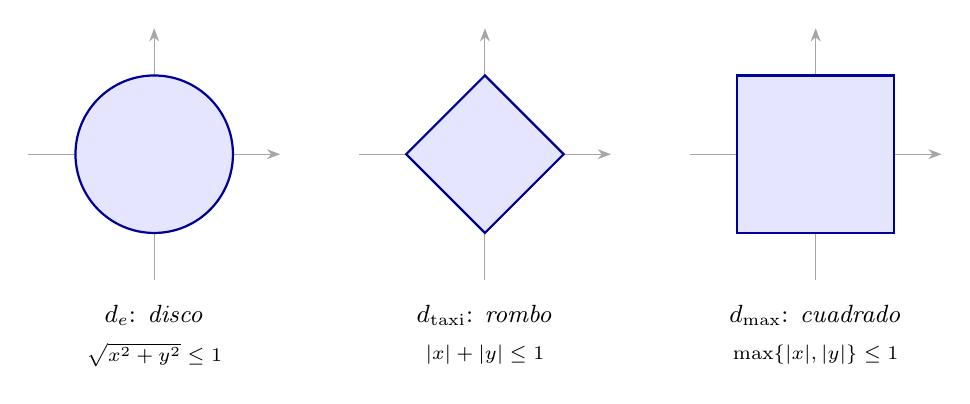
\begin{tikzpicture}[scale=1.0]
% euclidea
\begin{scope}
\draw[ejes] (-1.6,0)--(1.6,0); \draw[ejes] (0,-1.6)--(0,1.6);
\draw[abierto] (0,0) circle (1);
\node at (0,-2.05) {\small $d_e$: \emph{disco}};
\node at (0,-2.55) {\scriptsize $\sqrt{x^2+y^2}\le 1$};
\end{scope}
% taxi
\begin{scope}[xshift=4.2cm]
\draw[ejes] (-1.6,0)--(1.6,0); \draw[ejes] (0,-1.6)--(0,1.6);
\draw[abierto] (1,0)--(0,1)--(-1,0)--(0,-1)--cycle;
\node at (0,-2.05) {\small $d_{\text{taxi}}$: \emph{rombo}};
\node at (0,-2.55) {\scriptsize $|x|+|y|\le 1$};
\end{scope}
% max
\begin{scope}[xshift=8.4cm]
\draw[ejes] (-1.6,0)--(1.6,0); \draw[ejes] (0,-1.6)--(0,1.6);
\draw[abierto] (-1,-1) rectangle (1,1);
\node at (0,-2.05) {\small $d_{\max}$: \emph{cuadrado}};
\node at (0,-2.55) {\scriptsize $\max\{|x|,|y|\}\le 1$};
\end{scope}
\end{tikzpicture}
\figtit{Figura 1. Las bolas cerradas $B[(0,0),1]$ de las tres métricas de referencia en $\R^2$. En $\R^3$ las mismas fórmulas dan la esfera sólida, el octaedro y el cubo $[-1,1]^3$ (Métricos--C.1).}
\end{figure}

\begin{intuicion}
Las tres bolas son distintas \emph{como conjuntos}, pero cada una de las tres contiene una copia encogida de las otras dos alrededor del mismo centro: siempre se puede meter un rombito adentro de un disquito y un disquito adentro de un cuadradito. Eso es \emph{exactamente} lo que significa que las tres métricas den la misma topología (Prop.~\ref{pr:equiv}): la topología no ve la forma de la bola, solo ve ``qué conjuntos contienen una bolita alrededor de cada uno de sus puntos''.
\end{intuicion}

\begin{ejemplo}[Distancia discreta \fnt{GT 1.1.16, p.\,7}]
$d_D(x,y)=1$ si $x\ne y$ y $0$ si $x=y$. Es la métrica que induce la topología discreta.
\end{ejemplo}

\begin{proposicion}[La discreta no proviene de una norma \fnt{GT 1.1.17, p.\,7}]
No existe ninguna norma en $\R^n$ cuya distancia asociada sea la discreta.
\lgc{\neg\,\exists\,\norm{\cdot}\ \text{norma en }\R^n:\ \forall x,y\in\R^n\ \ \norm{x-y}=d_D(x,y).}
\end{proposicion}

\begin{proof}
Si $d_D(v,w)=\norm{v-w}$, tomo $v\ne 0$, con lo cual $\norm{v}=d_D(v,0)=1$. Pero entonces $\norm{\tfrac12 v}=\tfrac12\norm{v}=\tfrac12$, valor que $d_D$ nunca toma. La obstrucción es la \emph{homogeneidad}: una norma obliga a que el conjunto de distancias sea cerrado bajo multiplicación por escalares positivos.
\end{proof}


\subsection{Producto interno}

\begin{definicion}[Producto interno \fnt{EJ, Ejercicio teórico N$^\circ$1, p.\,3}]
Sobre un $\R$-espacio vectorial $V$, $(\cdot,\cdot):V\times V\to\R$ es un \emph{producto interno} si, para todos $u,v,w\in V$ y $\alpha\in\R$:
\begin{lista}
\item $(u,u)\ge 0$;
\item $(u,u)=0\iff u=0$;
\item $(u,v)=(v,u)$ (simetría);
\item $(u,v+w)=(u,v)+(u,w)$;
\item $(\alpha u,v)=\alpha\,(u,v)$.
\end{lista}
Se define $\norm{u}=\sqrt{(u,u)}$.
\lgc{(\cdot,\cdot)\ \text{es producto interno}\iff \forall u,v,w\in V\ \forall\alpha\in\R:\
(u,u)\ge0\ \wedge\ \big((u,u)=0\Leftrightarrow u=0\big)\\
\wedge\ (u,v)=(v,u)\ \wedge\ (u,v+w)=(u,v)+(u,w)\ \wedge\ (\alpha u,v)=\alpha\,(u,v);\qquad
\norm{u}:=\sqrt{(u,u)}.}
\end{definicion}

\begin{teorema}[Desigualdad de Cauchy--Schwarz \fnt{EJ, Ej.\ teórico N$^\circ$1.1, p.\,3}]
Sea $V$ un $\R$-espacio vectorial con producto interno $(\cdot,\cdot)$ y sea $\norm{u}=\sqrt{(u,u)}$. Entonces $|(u,v)|\le \norm{u}\,\norm{v}$ para todos $u,v\in V$.
\lgc{\forall u,v\in V:\quad |(u,v)|\le\norm{u}\,\norm{v}.}
\end{teorema}

\begin{proof}
Si $v=0$ es trivial. Si $v\ne 0$, para todo $t\in\R$:
\[
0\le (u+tv,\,u+tv)=\norm{u}^2+2t\,(u,v)+t^2\norm{v}^2 .
\]
Es un polinomio real de grado $2$ en $t$ no negativo, luego su discriminante es $\le 0$:
$4(u,v)^2-4\norm{u}^2\norm{v}^2\le 0$. (Alternativamente, evaluar en $t=-(u,v)/\norm{v}^2$.)
\end{proof}

\begin{corolario}[Norma asociada \fnt{EJ, Ej.\ teórico N$^\circ$1.2, p.\,3}]
Sobre un espacio con producto interno, $\norm{u}=\sqrt{(u,u)}$ es una norma; la desigualdad triangular sale de Cauchy--Schwarz vía
$\norm{u+v}^2=\norm{u}^2+2(u,v)+\norm{v}^2\le(\norm{u}+\norm{v})^2$.
\lgc{\norm{u}=\sqrt{(u,u)}\ \text{es norma};\qquad
\norm{u+v}^2=\norm{u}^2+2(u,v)+\norm{v}^2\le\big(\norm{u}+\norm{v}\big)^2.}
\end{corolario}


\begin{proposicion}[Identidad de polarización \fnt{EJ, Ej.\ teórico N$^\circ$1.4, p.\,3}]
Sea $V$ con producto interno y $\norm{\cdot}$ su norma asociada. Entonces $(u,v)=\tfrac14\norm{u+v}^2-\tfrac14\norm{u-v}^2$ para todos $u,v\in V$. Una norma proviene de un producto interno si y sólo si la fórmula anterior define un producto interno; equivalentemente, si y sólo si cumple la \emph{ley del paralelogramo}
$\norm{u+v}^2+\norm{u-v}^2=2\norm{u}^2+2\norm{v}^2$.
\lgc{(u,v)=\tfrac14\norm{u+v}^2-\tfrac14\norm{u-v}^2;\\
\norm{\cdot}\ \text{proviene de un producto interno}\iff \forall u,v:\ \norm{u+v}^2+\norm{u-v}^2=2\norm{u}^2+2\norm{v}^2.}
\end{proposicion}


\subsection{Fabricación de métricas nuevas}

Tres de los ejercicios de la guía A son casos particulares de dos principios generales; conviene estudiarlos así y no uno por uno.

\begin{lema}[Deformación por función cóncava \fnt{principio detrás de EJ, Métricos--A.1 y A.2, p.\,1}]
Sea $f:[0,\infty)\to[0,\infty)$ tal que $f(t)=0\iff t=0$, $f$ es creciente y \emph{subaditiva} ($f(a+b)\le f(a)+f(b)$). Si $d$ es una distancia en $X$, entonces $f\circ d$ también lo es.
\lgc{\Big[f\ \text{creciente}\ \wedge\ \forall a,b\ f(a+b)\le f(a)+f(b)\ \wedge\ \big(f(t)=0\Leftrightarrow t=0\big)\Big]\ \Rightarrow\ f\circ d\ \text{es distancia}.}
\end{lema}

\begin{proof}
Positividad, anulación y simetría son inmediatas. Para la triangular:
$f(d(x,y))\le f\big(d(x,z)+d(z,y)\big)\le f(d(x,z))+f(d(z,y))$, donde la primera desigualdad usa que $f$ es creciente y la segunda que es subaditiva.
\end{proof}


\begin{lema}[Métrica inducida por una inyección \fnt{principio detrás de EJ, Métricos--A.3, p.\,1}]
Sean $f:X\to Y$ una función y $(Y,\rho)$ métrico. Entonces $d(x,x'):=\rho(f(x),f(x'))$ es siempre una seudodistancia en $X$, y es una distancia si y sólo si $f$ es inyectiva.
\lgc{d(x,x'):=\rho\big(f(x),f(x')\big)\ \text{es seudodistancia};\qquad
d\ \text{es distancia}\iff f\ \text{es inyectiva}.}
\end{lema}





\subsection{Distancias entre funciones}\label{hu:secfunc}

\begin{proposicion}[Norma del supremo \fnt{GT Ej.\ 1.1.11, pp.\,4--5}]\label{hu:supnorm}
Sea $\ell^\infty(\R)=\{f:\R\to\R:\ f \text{ acotada}\}$, que es un $\R$-espacio vectorial con la suma y el producto por escalares punto a punto. Entonces $\norm{f}_\infty=\sup\{|f(x)|: x\in\R\}$ es una norma sobre $\ell^\infty(\R)$ (la \emph{norma del supremo}), y su distancia asociada es la \emph{distancia del supremo} $d_\infty(f,g)=\sup\{|f(x)-g(x)|: x\in\R\}$: dos funciones están a distancia menor que $\varepsilon$ cuando sus gráficos están ``uniformemente'' cerca.
\lgc{\norm{f}_\infty=\sup_{x\in\R}|f(x)|\ \ \text{es norma en } \ell^\infty(\R);\qquad d_\infty(f,g)=\sup_{x\in\R}|f(x)-g(x)|.}
\end{proposicion}

\begin{proof}
El supremo existe porque $f$ es acotada. $\norm{f}_\infty\ge0$ por ser supremo de valores absolutos; $\norm{\lambda f}_\infty=\sup|\lambda||f(x)|=|\lambda|\norm{f}_\infty$; si $\norm{f}_\infty=0$, entonces $0\le|f(x)|\le 0$ para todo $x$ y $f$ es la función nula $\theta$. Triangular: para cada $x$, $|f(x)+g(x)|\le|f(x)|+|g(x)|\le\norm{f}_\infty+\norm{g}_\infty$; como la cota no depende de $x$, también acota al supremo.
\end{proof}

\begin{ejemplo}[Cuentas con $d_\infty$ \fnt{GT Ej.\ 1.1.12, p.\,5}]
$\norm{\sin}_\infty=1$. Entre $\sin$ y $\cos$: $\sin x-\cos x=\sqrt2\,\sin(x-\tfrac\pi4)$, luego $d_\infty(\sin,\cos)=\sqrt2$ (se alcanza en $x=\tfrac{3\pi}4$). Si $f_n=\tfrac1n\sin$, entonces $d_\infty(f_n,\theta)=\tfrac1n\to0$: la sucesión se acerca tanto como se quiera a la función nula en $(\ell^\infty(\R),d_\infty)$.
\end{ejemplo}

\begin{observacion}[Errata de GT 1.1.12]
\textbf{GT} afirma $d_\infty(\sin,\cos)=1$; el valor correcto es $\sqrt2$, por la cuenta de arriba.
\end{observacion}

\begin{proposicion}[La norma integral \fnt{GT Ej.\ 1.1.13, pp.\,5--6}]\label{hu:norma1}
Sobre $C[0,1]=\{f:[0,1]\to\R:\ f \text{ continua}\}$, $\norm{f}_1=\int_0^1|f(x)|\,dx$ es una norma, con distancia asociada $d_1(f,g)=\int_0^1|f(x)-g(x)|\,dx$ (el área entre los dos gráficos).
\lgc{\norm{f}_1=\int_0^1|f(x)|\,dx\ \ \text{es norma en } C[0,1];\qquad d_1(f,g)=\int_0^1|f(x)-g(x)|\,dx.}
\end{proposicion}

\begin{proof}
Positividad y homogeneidad salen de las de la integral; la triangular, de integrar $|f(x)+g(x)|\le|f(x)|+|g(x)|$. La anulación es la que usa la \emph{continuidad}: si $f(x_0)\ne0$ para algún $x_0$, por continuidad $|f|\ge\tfrac12|f(x_0)|$ en un intervalo $I\ni x_0$ de longitud $\ell>0$ contenido en $[0,1]$, y entonces $\norm{f}_1\ge\tfrac12|f(x_0)|\,\ell>0$.
\end{proof}

\begin{observacion}[Sobre la demostración de GT 1.1.13 y las normas $\norm{\cdot}_p$]
En el punto 3, \textbf{GT} pasa de $\int_0^1|f|=0$ a $f\equiv0$ ``para todo $x\in\R$'' sin justificar: hace falta la continuidad (una función que vale $1$ en un solo punto y $0$ en el resto tiene integral nula) y el dominio es $[0,1]$. \textbf{GT} menciona además $\norm{f}_p=\big(\int_0^1|f|^p\big)^{1/p}$ (allí escrita con $n$); también es una norma, pero su triangular es la desigualdad de Minkowski, que no se demuestra en el curso.
\end{observacion}

\begin{observacion}[$d_1$ y $d_\infty$ miden cosas distintas \fnt{GT Ej.\ 1.1.14, p.\,6}]
En $C[0,1]$ vale $d_1\le d_\infty$ (se integra $|f-g|\le d_\infty(f,g)$ sobre un intervalo de longitud $1$), así que acercarse en $d_\infty$ obliga a acercarse en $d_1$. Al revés no: una sucesión de ``picos'' de altura $1$ y base cada vez más angosta tiende a $\theta$ en $d_1$ y se queda a distancia $1$ de $\theta$ en $d_\infty$.
\end{observacion}

\begin{ejemplo}[Una seudodistancia: la llegada a la meta \fnt{GT Ej.\ 1.1.15, pp.\,6--7}]\label{hu:dmeta}
En $C[0,1]$, $d_{\text{meta}}(f,g)=|f(1)-g(1)|$ es una seudodistancia que no es distancia: dos funciones distintas que coinciden en $1$ están a distancia $0$. Es el Lema de la métrica inducida (\S\ref{sec:metricos}) aplicado a la evaluación $f\mapsto f(1)$, de $C[0,1]$ en $(\R,|\cdot|)$, que no es inyectiva. Lectura de \textbf{GT}: si $f$ creciente con $f(0)=0$ da el tiempo en que un corredor pasa por cada punto de la pista $[0,1]$, $d_{\text{meta}}$ sólo compara los tiempos de llegada.
\lgc{d_{\text{meta}}(f,g)=|f(1)-g(1)|;\qquad f\ne g\ \wedge\ f(1)=g(1)\ \Rightarrow\ d_{\text{meta}}(f,g)=0.}
\end{ejemplo}

\subsection{Distancia a un conjunto, diámetro, acotación}

\begin{definicion}[\fnt{curso; usada en EJ, Métricos--A.7 y A.9, p.\,2, y Continuidad--A.3, p.\,12}]
Dados $(X,d)$, subconjuntos no vacíos $A,B\subseteq X$ y $x\in X$:
\begin{lista}
\item distancia de un punto a un conjunto: $d(x,A)=\inf\{d(x,a):a\in A\}$;
\item distancia entre conjuntos: $d(A,B)=\inf\{d(a,b):a\in A,\ b\in B\}$;
\item diámetro: $\delta(A)=\sup\{d(a,b):a,b\in A\}$;
\item $A$ es \emph{acotado} si $\delta(A)<\infty$.
\end{lista}
\lgc{d(x,A)=\inf\{d(x,a):a\in A\};\qquad d(A,B)=\inf\{d(a,b):a\in A,\ b\in B\};\\
\delta(A)=\sup\{d(a,b):a,b\in A\};\qquad A\ \text{acotado}\iff \delta(A)<\infty.}
\end{definicion}

\begin{observacion}[Por qué ínfimo y no mínimo]
$d(x,A)$ se define como un \emph{ínfimo} porque el mínimo puede no existir: en $\R$ con $A=(0,1)$ y $x=0$, ninguna $a\in A$ realiza la distancia, y sin embargo $d(0,A)=0$. Las dos cosas que se usan en toda demostración con $d(x,A)$ son:
\begin{lista}
\item $d(x,A)\le d(x,a)$ para todo $a\in A$ (es cota inferior);
\item para todo $\varepsilon>0$ existe $a\in A$ con $d(x,a)<d(x,A)+\varepsilon$ (es la \emph{mayor} cota inferior, así que $d(x,A)+\varepsilon$ ya no lo es).
\end{lista}
La primera sirve para acotar hacia abajo; la segunda, para fabricar el punto $a$ que hace falta. Lo mismo, dado vuelta, para el supremo en $\delta(A)$. Y es exactamente por esto que $d(x,A)=0$ no obliga a que $x$ esté en $A$: sólo dice que hay puntos de $A$ tan cerca como se quiera, es decir que $x\in\cl A$.
\end{observacion}

\begin{proposicion}[$d(\cdot,A)$ es $1$-lipschitziana \fnt{EJ, Métricos--A.7, p.\,2; Continuidad--A.3, p.\,12}]\label{pr:lip}
Para todos $x,y\in X$: $|d(x,A)-d(y,A)|\le d(x,y)$. En consecuencia, $x\mapsto d(x,A)$ es uniformemente continua.
\lgc{\forall x,y\in X:\ \big|d(x,A)-d(y,A)\big|\le d(x,y);\\
\forall\varepsilon>0\ \exists\delta>0\ \forall x,y:\ d(x,y)<\delta\Rightarrow \big|d(x,A)-d(y,A)\big|<\varepsilon.}
\end{proposicion}

\begin{proof}
Para todo $a\in A$: $d(x,A)\le d(x,a)\le d(x,y)+d(y,a)$. Tomando ínfimo sobre $a\in A$ en el miembro derecho, $d(x,A)\le d(x,y)+d(y,A)$, es decir $d(x,A)-d(y,A)\le d(x,y)$. Intercambiando $x$ e $y$ se obtiene la otra desigualdad. Para la continuidad uniforme basta $\delta=\varepsilon$.
\end{proof}

\begin{figure}[ht]
\centering
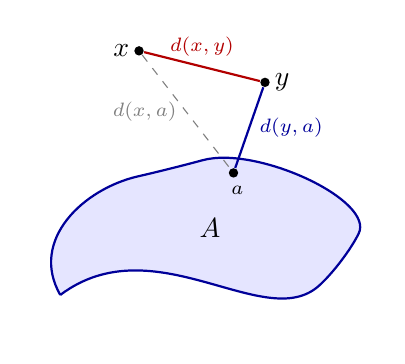
\begin{tikzpicture}[scale=1.0]
\draw[abierto,rounded corners=12pt] (0,0) .. controls (1.2,0.9) and (2.6,-0.5) .. (3.6,0.4)
 .. controls (4.0,1.2) and (2.5,1.9) .. (1.4,1.6) .. controls (0.3,1.35) and (-0.4,0.7) .. (0,0);
\node at (1.9,0.85) {$A$};
\node[pt] (x) at (1.0,3.1) {}; \node[left] at (1.0,3.1) {$x$};
\node[pt] (y) at (2.6,2.7) {}; \node[right] at (2.6,2.7) {$y$};
\node[pt] (a) at (2.2,1.55) {}; \node[below] at (2.25,1.5) {\scriptsize $a$};
\draw[red!70!black,thick] (x)--(y) node[midway,above]{\scriptsize $d(x,y)$};
\draw[blue!60!black,thick] (y)--(a) node[midway,right]{\scriptsize $d(y,a)$};
\draw[gray,dashed] (x)--(a) node[midway,left]{\scriptsize $d(x,a)$};
\end{tikzpicture}
\figtit{Figura 2. Para \emph{cualquier} $a\in A$ el camino $x\to y\to a$ acota a $d(x,A)$. Como la cota vale para todo $a$, sobrevive al tomar ínfimo.}
\end{figure}

\begin{intuicion}
La función $x\mapsto d(x,A)$ mide ``a qué distancia estoy del conjunto $A$''. La proposición dice que si me muevo $10$ metros, mi distancia a $A$ cambia a lo sumo $10$ metros: no puede haber saltos. Ese es el contenido geométrico de \emph{lipschitziana}, y la continuidad uniforme sale gratis porque el $\delta$ que sirve ($\delta=\varepsilon$) no depende del punto.
\end{intuicion}



\subsection{Bolas}\label{sec:bolas}

\begin{definicion}[\fnt{GT 1.1.18, p.\,8}]
$\Bola{x}{\varepsilon}=\{y\in X: d(x,y)<\varepsilon\}$ (bola abierta), $\Bolac{x}{\varepsilon}=\{y: d(x,y)\le\varepsilon\}$ (bola cerrada).
\lgc{\Bola{x}{\varepsilon}=\{y\in X:\ d(x,y)<\varepsilon\};\qquad
\Bolac{x}{\varepsilon}=\{y\in X:\ d(x,y)\le\varepsilon\}.}
\end{definicion}

\begin{ejemplo}[Bolas de referencia \fnt{GT Ejs.\ 1.1.19--1.1.24, pp.\,8--10}]\label{hu:bolas}
\begin{lista}
\item En $(\R,|\cdot|)$: $\Bola{x}{\varepsilon}=(x-\varepsilon,x+\varepsilon)$ \fnt{GT 1.1.19}.
\item En $(\R^2,d_e)$: $\Bola{0}{\varepsilon}=\{(x_1,x_2): x_1^2+x_2^2<\varepsilon^2\}$, el disco sin su circunferencia \fnt{GT 1.1.20}.
\item En $(\R^2,d_{\text{taxi}})$: $\Bola{0}{\varepsilon}=\{|x_1|+|x_2|<\varepsilon\}$, el cuadrado girado (rombo) sin borde con vértices $(\pm\varepsilon,0)$, $(0,\pm\varepsilon)$; se ve separando los cuatro cuadrantes, donde la condición es $\pm x_1\pm x_2<\varepsilon$ \fnt{GT 1.1.21}.
\item En $(\R^2,d_{\max})$: $\Bola{0}{\varepsilon}=\{|x_1|<\varepsilon,\ |x_2|<\varepsilon\}=(-\varepsilon,\varepsilon)^2$, el cuadrado sin borde de lado $2\varepsilon$ y lados paralelos a los ejes \fnt{GT 1.1.22}.
\item En $(\ell^\infty(\R),d_\infty)$: $B_{d_\infty}(\theta,\varepsilon)=\{f:\ \sup|f|<\varepsilon\}$ son las funciones cuyo gráfico queda dentro de una franja $[-\varepsilon',\varepsilon']$ con $\varepsilon'<\varepsilon$ \fnt{GT 1.1.23}.
\item En $(\R^2,d_D)$ (discreta): $\Bola{\theta}{\varepsilon}=\{\theta\}$ si $\varepsilon\le1$ y $\Bola{\theta}{\varepsilon}=\R^2$ si $\varepsilon>1$ \fnt{GT 1.1.24}.
\end{lista}
\lgc{B_{d_\infty}(\theta,\varepsilon)=\{f:\ \sup_x|f(x)|<\varepsilon\}\subsetneq\{f:\ \forall x\ |f(x)|<\varepsilon\};\qquad
B_{d_D}(\theta,\varepsilon)=\begin{cases}\{\theta\}&\varepsilon\le1\\ \R^2&\varepsilon>1.\end{cases}}
\end{ejemplo}

\begin{observacion}[Erratas de GT 1.1.20 y 1.1.23]
En 1.1.20 el paso intermedio dice $x_1^2+x_2^2<\varepsilon$; es $\sqrt{x_1^2+x_2^2}<\varepsilon$, y el resultado final ($<\varepsilon^2$) es el correcto. En 1.1.23, \textbf{GT} identifica $B_{d_\infty}(\theta,\varepsilon)$ con ``$-\varepsilon<f(x)<\varepsilon$ para todo $x$'' (escrito allí con $|f(x)|$), que es un conjunto \emph{más grande}: $f(x)=\varepsilon\,\frac{x^2}{1+x^2}$ cumple $|f(x)|<\varepsilon$ en todo punto, pero $\sup|f|=\varepsilon$, así que $f\notin B_{d_\infty}(\theta,\varepsilon)$. Pedir que el supremo sea $<\varepsilon$ es pedir un margen uniforme: el gráfico tiene que caber en una franja estrictamente más angosta.
\end{observacion}

\begin{figure}[ht]
\centering
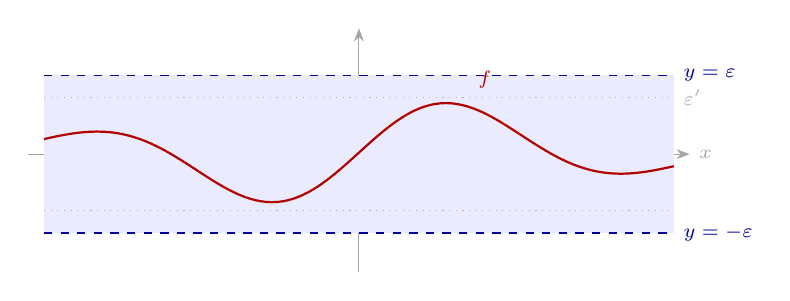
\begin{tikzpicture}[scale=1.0]
\draw[ejes] (-4.2,0)--(4.2,0) node[right]{\scriptsize $x$};
\draw[ejes] (0,-1.5)--(0,1.6);
\fill[blue!8] (-4,-1) rectangle (4,1);
\draw[blue!60!black,dashed] (-4,1)--(4,1) node[right]{\scriptsize $y=\varepsilon$};
\draw[blue!60!black,dashed] (-4,-1)--(4,-1) node[right]{\scriptsize $y=-\varepsilon$};
\draw[gray!60,dotted] (-4,0.72)--(4,0.72) node[right]{\scriptsize $\varepsilon'$};
\draw[gray!60,dotted] (-4,-0.72)--(4,-0.72);
\draw[red!70!black,thick,domain=-4:4,samples=120] plot (\x,{0.7*sin(deg(1.3*\x))*exp(-0.08*\x*\x)+0.02});
\node[red!70!black] at (1.6,0.95) {\scriptsize $f$};
\end{tikzpicture}
\figtit{Figura 3. Una $f$ en la bola $B_{d_\infty}(\theta,\varepsilon)$: su gráfico no sólo queda entre $y=-\varepsilon$ e $y=\varepsilon$, sino dentro de una franja más angosta $[-\varepsilon',\varepsilon']$. Una función que se acerca a la recta $y=\varepsilon$ sin tocarla está a distancia exactamente $\varepsilon$ de $\theta$.}
\end{figure}

\begin{proposicion}[Propiedades de las bolas \fnt{GT 1.1.25, p.\,10}]
En $(X,d)$:
\begin{lista}
\item $x\in\Bola{x}{\varepsilon}$;
\item si $y\in\Bola{x}{\varepsilon}$, existe $\delta>0$ con $\Bola{y}{\delta}\subseteq\Bola{x}{\varepsilon}$ (sirve $\delta=\varepsilon-d(x,y)$);
\item $\Bola{x}{\varepsilon_1}\cap\Bola{x}{\varepsilon_2}=\Bola{x}{\min\{\varepsilon_1,\varepsilon_2\}}$.
\end{lista}
\lgc{x\in\Bola{x}{\varepsilon};\qquad
\forall y\in\Bola{x}{\varepsilon}\ \exists\delta>0:\ \Bola{y}{\delta}\subseteq\Bola{x}{\varepsilon};\\
\Bola{x}{\varepsilon_1}\cap\Bola{x}{\varepsilon_2}=\Bola{x}{\min\{\varepsilon_1,\varepsilon_2\}}.}
\end{proposicion}

\begin{teorema}[Separación de Hausdorff en métricos \fnt{GT 1.1.26, p.\,11; MS Teo.\ 2.13, p.\,32}]
Si $(X,d)$ es métrico y $x\ne x'$, existe $\varepsilon>0$ con $\Bola{x}{\varepsilon}\cap\Bola{x'}{\varepsilon}=\emptyset$ (basta $\varepsilon=d(x,x')/2$).
\lgc{\forall x\ne x'\ \exists\varepsilon>0:\ \Bola{x}{\varepsilon}\cap\Bola{x'}{\varepsilon}=\emptyset\qquad(\text{sirve } \varepsilon=\tfrac{d(x,x')}{2}).}
\end{teorema}

\begin{ejemplo}[En un seudométrico la separación puede fallar \fnt{GT Ej.\ 1.1.27, p.\,11}]\label{hu:seudoR2}
En $\R^2$, $d\big((x,x'),(y,y')\big)=|x-y|$ es una seudodistancia (la inducida por la proyección $p_1$, que no es inyectiva) y no una distancia: $d\big((0,0),(0,1)\big)=0$. Por eso $(0,1)\in\Bola{(0,0)}{\varepsilon}$ para todo $\varepsilon>0$, y ninguna bola de $(0,0)$ es disjunta de ninguna bola de $(0,1)$: los dos puntos no se pueden separar. En general $\Bola{(a,b)}{\varepsilon}=(a-\varepsilon,a+\varepsilon)\times\R$ es una franja vertical, que no distingue puntos de una misma recta vertical. El teorema anterior usa de verdad que $d(x,x')>0$ para $x\ne x'$.
\lgc{d\big((0,0),(0,1)\big)=0\ \Rightarrow\ \forall\varepsilon>0:\ \Bola{(0,0)}{\varepsilon}\cap\Bola{(0,1)}{\varepsilon}\ni(0,1).}
\end{ejemplo}



%======================================================================
\section{La topología de un espacio métrico}\label{sec:topmet}

\begin{definicion}[Interior, abierto, entorno \fnt{GT 1.2.1, p.\,12}]
$x$ es \emph{punto interior} de $A$ si existe $\varepsilon>0$ con $\Bola{x}{\varepsilon}\subseteq A$; $\intr A$ es el conjunto de tales puntos. $A$ es \emph{abierto} si $A=\intr A$, y $N$ es \emph{entorno} de $x$ si $x\in\intr N$.
\lgc{x\in\intr A\iff \exists\varepsilon>0:\ \Bola{x}{\varepsilon}\subseteq A;\\
A\ \text{abierto}\iff A=\intr A;\qquad N\in\mathcal N_x\iff x\in\intr N.}
\end{definicion}

\begin{proposicion}[\fnt{GT 1.2.2 y 1.2.6, pp.\,12 y 15}]
En $(X,d)$:
\begin{lista}
\item $\intr A\subseteq A$;
\item toda bola abierta es un conjunto abierto;
\item $A$ es abierto $\iff$ $A$ es entorno de todos sus puntos;
\item $N$ es entorno de $x$ $\iff$ existe un abierto $G$ con $x\in G\subseteq N$;
\item $x\in\intr A$ $\iff$ existe un abierto $G$ con $x\in G\subseteq A$.
\end{lista}
\lgc{\intr A\subseteq A;\qquad \Bola{x}{\varepsilon}\ \text{es abierta};\qquad
A\ \text{abierto}\iff \forall x\in A:\ A\in\mathcal N_x;\\
N\in\mathcal N_x\iff \exists G\ \text{abierto}:\ x\in G\subseteq N;\qquad
x\in\intr A\iff \exists G\ \text{abierto}:\ x\in G\subseteq A.}
\end{proposicion}

\begin{proposicion}[Propiedades del interior \fnt{GT 1.2.7, p.\,15}]
Sea $(X,d)$ y sean $A,B,A_1,\dots,A_n\subseteq X$:
\begin{lista}
\item $\intr A\subseteq A$;
\item si $A\subseteq B$ entonces $\intr A\subseteq\intr B$;
\item $\intr(A_1\cap\dots\cap A_n)=\intr A_1\cap\dots\cap\intr A_n$;
\item $\intr(\intr A)=\intr A$.
\end{lista}
\lgc{\intr A\subseteq A;\qquad A\subseteq B\Rightarrow\intr A\subseteq\intr B;\\
\intr\Big(\bigcap_{k=1}^{n}A_k\Big)=\bigcap_{k=1}^{n}\intr A_k;\qquad \intr(\intr A)=\intr A.}
\end{proposicion}

\begin{teorema}[Propiedades básicas de los abiertos \fnt{GT 1.2.8, p.\,16; GT Ej.\ 2.1.2, p.\,18}]
En $(X,d)$:
\begin{lista}
\item $\emptyset$ y $X$ son abiertos;
\item la intersección \emph{finita} de abiertos es abierta;
\item la unión \emph{arbitraria} de abiertos es abierta.
\end{lista}
Estas tres propiedades son exactamente las que se axiomatizan al definir topología.
\lgc{\emptyset,X\in\tp_d;\qquad G_1,\dots,G_n\in\tp_d\Rightarrow\bigcap_{k=1}^{n}G_k\in\tp_d;\qquad
\{G_i\}_{i\in I}\subseteq\tp_d\Rightarrow\bigcup_{i\in I}G_i\in\tp_d.}
\end{teorema}

\begin{proposicion}[Métricas equivalentes en $\R^n$ \fnt{GT 1.2.3--1.2.4, pp.\,13--14; GT Nota 2.1.3, p.\,19}]\label{pr:equiv}
$d_e$, $d_{\text{taxi}}$ y $d_{\max}$ tienen exactamente los mismos abiertos; la clave son las inclusiones entre bolas del tipo
$B_{d_{\max}}(x,\varepsilon/2)\subseteq B_{d_e}(x,\sqrt2\,\varepsilon/2)\subseteq B_{d_{\text{taxi}}}(x,\varepsilon)$. Por lo tanto $\tp_{d_e}=\tp_{d_{\text{taxi}}}=\tp_{d_{\max}}$: distancias distintas pueden dar la misma topología, y esa es la observación que motiva todo el capítulo siguiente.
\lgc{\tp_{d_e}=\tp_{d_{\text{taxi}}}=\tp_{d_{\max}}.}
\end{proposicion}

\begin{proposicion}[El caso de $\R^n$ \fnt{GT 1.2.3--1.2.4 y Nota 1.2.5, pp.\,13--14}]\label{hu:equivRn}
En $\R^n$ las tres distancias se comparan así: la del máximo es la menor, la del taxi la mayor, y la del taxi no supera $n$ veces la del máximo. En consecuencia las bolas encajan unas en otras, cada bola de una de las tres métricas es abierta para las otras dos, y las tres topologías coinciden.
\lgc{d_{\max}\le d_e\le d_{\text{taxi}}\le n\,d_{\max};\\
B_{d_{\text{taxi}}}(x,\varepsilon)\subseteq B_{d_e}(x,\varepsilon)\subseteq B_{d_{\max}}(x,\varepsilon)\subseteq B_{d_{\text{taxi}}}(x,n\varepsilon);\qquad
\tp_{d_e}=\tp_{d_{\text{taxi}}}=\tp_{d_{\max}}.}
\end{proposicion}

\begin{proof}
Sea $u_i=|x_i-y_i|$ y $M=\max_i u_i$. Como $M$ es uno de los $u_i$: $M^2\le\sum_iu_i^2$, o sea $d_{\max}\le d_e$. Desarrollando el cuadrado, $\big(\sum_iu_i\big)^2=\sum_iu_i^2+\sum_{i\ne j}u_iu_j\ge\sum_iu_i^2$, o sea $d_e\le d_{\text{taxi}}$. Y $\sum_iu_i\le nM$. Las inclusiones de bolas son estas desigualdades leídas al revés (si la distancia mayor es $<\varepsilon$, la menor también). Para las topologías: si $A$ es abierto para una de las métricas y $x\in A$, hay una bola de esa métrica alrededor de $x$ dentro de $A$, y la cadena de inclusiones mete dentro de ella una bola de cualquiera de las otras dos (achicando el radio a $\varepsilon/n$ cuando hace falta). Luego $x$ es interior a $A$ en las tres. Como corolario, cada bola de una métrica, al ser abierta en ella, es abierta en las otras dos (GT 1.2.4).
\end{proof}

\subsection{Adherencia, frontera y cerrados en un espacio métrico}

\noindent Estas nociones se definen en general para espacios topológicos (\S\ref{sec:top}); en un espacio métrico todas se leen con bolas, y esa es la forma en que aparecen en los ejercicios y en los parciales. Cada enunciado de acá es el de \S\ref{sec:top} con ``todo abierto que contiene a $x$'' reemplazado por ``toda bola de centro $x$'', que es lo mismo porque las bolas son base local.

\begin{definicion}[Punto adherente, clausura \fnt{GT 2.3.4 y 2.3.6, pp.\,22--23, leídos con bolas}]
$x$ es \emph{adherente} a $A$ si toda bola de centro $x$ corta a $A$. La \emph{clausura} (o \emph{adherencia}) $\cl A$ es el conjunto de los puntos adherentes a $A$.
\lgc{x\in\cl A\iff \forall\varepsilon>0:\ \Bola{x}{\varepsilon}\cap A\ne\emptyset.}
\end{definicion}

\begin{definicion}[Punto de acumulación, punto aislado \fnt{GT 2.2.7 y 2.3.1, pp.\,21--22, leídos con bolas}]
$x$ es de \emph{acumulación} de $A$ si toda bola de centro $x$ corta a $A$ en algún punto distinto de $x$; el conjunto de todos ellos es el \emph{derivado} $A'$. Un punto $x\in A$ es \emph{aislado} si alguna bola de centro $x$ no contiene otros puntos de $A$.
\lgc{x\in A'\iff \forall\varepsilon>0:\ \Bola{x}{\varepsilon}\cap\big(A-\{x\}\big)\ne\emptyset;\\
x\ \text{aislado de } A\iff x\in A\ \wedge\ \exists\varepsilon>0:\ \Bola{x}{\varepsilon}\cap A=\{x\}.}
\end{definicion}

\begin{proposicion}[En un métrico, acumular es tener infinitos puntos cerca \fnt{GT 2.3.2, pp.\,21--22}]\label{hu:acuminf}
Sea $(X,d)$ métrico, $A\subseteq X$ y $x\in X$. Entonces $x$ es punto de acumulación de $A$ si y sólo si todo abierto $G$ que contiene a $x$ contiene infinitos puntos de $A$ (equivalentemente, toda bola de centro $x$ contiene infinitos puntos de $A$).
\lgc{x\in A'\iff \forall G\in\tp_d\ \big(x\in G\Rightarrow G\cap A\ \text{es infinito}\big).}
\end{proposicion}

\begin{proof}
($\Leftarrow$) Si $G\ni x$ tiene infinitos puntos de $A$, al sacar $x$ quedan infinitos, así que $(G-\{x\})\cap A\ne\emptyset$.
($\Rightarrow$) Por el absurdo: sea $G\ni x$ abierto con $G\cap A$ finito. Entonces $F=(G\cap A)-\{x\}$ es finito. Tomo $r>0$ con $\Bola{x}{r}\subseteq G$ y, si $F=\{a_1,\dots,a_k\}\ne\emptyset$, lo achico para que además $r\le\min_i d(x,a_i)$, que es positivo porque cada $a_i\ne x$ y $d$ es distancia. Entonces $\big(\Bola{x}{r}-\{x\}\big)\cap A\subseteq F$ y ningún $a_i$ está en la bola (todos están a distancia $\ge r$): la intersección es vacía, contra $x\in A'$.
\end{proof}

\begin{observacion}[Sobre el enunciado y la hipótesis]
\textbf{GT} escribe ``todo abierto $G$'' donde debe decir ``todo abierto $G$ \emph{que contiene a} $x$''; y demuestra ($\Rightarrow$) fabricando una sucesión de puntos distintos con radios que se van achicando a la mitad, que es la misma idea. Lo que se usa del espacio métrico es que $d(x,a)>0$ si $a\ne x$ (en el fondo, que los finitos son cerrados). Sin eso falla: en $X=\{a,b\}$ indiscreto, $A=\{b\}$, el punto $a$ es de acumulación de $A$ y $A$ es finito. De esta proposición sale el Cor.\ 2.3.3: en un métrico, un conjunto finito no tiene puntos de acumulación, y todos sus puntos son aislados.
\end{observacion}

\begin{definicion}[Frontera y exterior \fnt{GT 2.6.1 y 2.6.4, p.\,29, leídos con bolas}]
$x\in\fr A$ si toda bola de centro $x$ corta a la vez a $A$ y a $X-A$. $x\in\ext A$ si alguna bola de centro $x$ no toca $A$.
\lgc{x\in\fr A\iff \forall\varepsilon>0:\ \Bola{x}{\varepsilon}\cap A\ne\emptyset\ \wedge\ \Bola{x}{\varepsilon}\cap(X-A)\ne\emptyset;\\
x\in\ext A\iff \exists\varepsilon>0:\ \Bola{x}{\varepsilon}\cap A=\emptyset.}
\end{definicion}

\begin{definicion}[Conjunto cerrado, conjunto denso \fnt{GT 1.2.8 y 2.6.7, pp.\,16 y 31}]
$C\subseteq X$ es \emph{cerrado} si $X-C$ es abierto. $D\subseteq X$ es \emph{denso} si toda bola de $X$ corta a $D$.
\lgc{C\ \text{cerrado}\iff X-C\in\tp_d;\qquad
D\ \text{denso}\iff \forall x\in X\ \forall\varepsilon>0:\ \Bola{x}{\varepsilon}\cap D\ne\emptyset\iff \cl D=X.}
\end{definicion}

\begin{proposicion}[La clausura, medida con la distancia \fnt{consecuencia de GT 1.1.18 y 2.3.4; parcial 2/10/2023, ej.\ 3}]
En un espacio métrico $(X,d)$, para todo $\emptyset\ne A\subseteq X$:
\[
\cl A=\{x\in X:\ d(x,A)=0\}.
\]
Equivalentemente, $x\notin\cl A\iff d(x,A)>0$.
\end{proposicion}

\begin{proof}
$\subseteq$: si $x\in\cl A$, toda bola $\Bola{x}{\varepsilon}$ corta a $A$, luego existe $a\in A$ con $d(x,a)<\varepsilon$; entonces $d(x,A)<\varepsilon$ para todo $\varepsilon>0$, o sea $d(x,A)=0$.
$\supseteq$: si $d(x,A)=0$, dado $\varepsilon>0$ el ínfimo no es cota inferior estricta, así que existe $a\in A$ con $d(x,a)<\varepsilon$; luego toda bola de centro $x$ corta a $A$ y $x$ es adherente. La clave es que $d(x,A)$ es un \emph{ínfimo}: vale $0$ sin necesidad de que se alcance, y por eso $x$ puede estar en $\cl A$ sin estar en $A$.
\end{proof}

\begin{corolario}
Sea $\emptyset\ne A\subseteq(X,d)$. Entonces $A$ es cerrado $\iff$ $\big(d(x,A)=0\Rightarrow x\in A\big)$ para todo $x\in X$. Y $\cl A=f^{-1}(0)$ para la función continua $f(x)=d(x,A)$, lo que da otra prueba de que la clausura es cerrada.
\end{corolario}

\begin{proposicion}[Caracterizaciones de ``cerrado'' en un métrico \fnt{GT 2.4.2, p.\,24; GT 2.5.6--2.5.7, p.\,28}]
Para $A\subseteq(X,d)$ son equivalentes:
\begin{lista}
\item $A$ es cerrado (su complemento es abierto);
\item $A=\cl A$, es decir $A$ contiene todos sus puntos adherentes;
\item $A'\subseteq A$, es decir $A$ contiene todos sus puntos de acumulación;
\item toda sucesión de puntos de $A$ que converge en $X$ tiene su límite en $A$;
\item $d(x,A)=0\Rightarrow x\in A$.
\end{lista}
\lgc{A\ \text{cerrado}\iff X-A\in\tp_d\iff A=\cl A\iff A'\subseteq A\\
\iff \forall\{a_n\}\subseteq A\ \big(a_n\to x\Rightarrow x\in A\big)
\iff \forall x\ \big(d(x,A)=0\Rightarrow x\in A\big).}
\end{proposicion}

\begin{intuicion}
Las cinco versiones dicen lo mismo desde ángulos distintos, y en un parcial conviene elegir la que menos cuentas pida: si el conjunto viene dado por una condición con $\le$ o $\ge$, sale por complemento abierto; si viene de un límite o de una sucesión, por (4); si aparece una distancia, por (5). En espacios topológicos generales sólo sobreviven (1), (2) y (3): la (4) y la (5) necesitan la métrica.
\end{intuicion}

\begin{proposicion}[Supremo e ínfimo son adherentes \fnt{GT Ej.\ 2.3.7, p.\,23}]\label{hu:supadh}
Sea $\emptyset\ne A\subseteq(\R,|\cdot|)$. Si $A$ está acotado inferiormente, su ínfimo es adherente a $A$; si está acotado superiormente, su supremo es adherente a $A$. En particular, un cerrado no vacío y acotado de $\R$ tiene mínimo y máximo.
\lgc{A\ne\emptyset\ \text{acotado inferiormente}\Rightarrow \inf A\in\cl A;\qquad A\ne\emptyset\ \text{acotado superiormente}\Rightarrow \sup A\in\cl A;\\
A\ne\emptyset\ \text{cerrado y acotado}\Rightarrow \inf A=\min A\ \wedge\ \sup A=\max A.}
\end{proposicion}

\begin{proof}
Sea $x_0=\inf A$ y $\varepsilon>0$. Como $x_0+\varepsilon$ ya no es cota inferior, hay $a\in A$ con $x_0\le a<x_0+\varepsilon$; entonces $a\in\Bola{x_0}{\varepsilon}\cap A$. Toda bola de centro $x_0$ corta a $A$, o sea $x_0\in\cl A$. Con el supremo es igual, con $a\in A$ tal que $\sup A-\varepsilon<a\le\sup A$. Si además $A$ es cerrado, $\cl A=A$ y el ínfimo y el supremo son elementos de $A$, es decir, mínimo y máximo.
\end{proof}

\begin{observacion}
Es exactamente la segunda propiedad del ínfimo de la Observación ``Por qué ínfimo y no mínimo'', leída como ``toda bola corta a $A$''. Se usa en la prueba de que $[a,b]$ es conexo (\S\ref{sec:bolzano}). La demostración de \textbf{GT} tiene dos descuidos de tipeo: escribe $a_{\varepsilon/2}$ donde va $a_{\varepsilon_0/2}$, y concluye ``$x_0\in A$'' donde va $x_0\in\cl A$.
\end{observacion}

%======================================================================
\section{Espacios topológicos}\label{sec:top}

\begin{definicion}[Topología \fnt{GT 2.1.1, p.\,18; MS Def.\ 2.1, p.\,23}]
$\tp\subseteq\mathcal{P}(X)$ es una \emph{topología} si:
\begin{lista}
\item $\emptyset,X\in\tp$;
\item $\tp$ es cerrada por intersecciones finitas;
\item $\tp$ es cerrada por uniones arbitrarias.
\end{lista}
Los elementos de $\tp$ son los \emph{abiertos}; $C\subseteq X$ es \emph{cerrado} si $X-C\in\tp$.
\lgc{\tp\ \text{topología}\iff \emptyset,X\in\tp\ \wedge\ \Big(\{G_i\}_{i\in I}\subseteq\tp\Rightarrow\bigcup_{i\in I}G_i\in\tp\Big)
\ \wedge\ \Big(G_1,\dots,G_n\in\tp\Rightarrow\bigcap_{k=1}^{n}G_k\in\tp\Big);\\
C\ \text{cerrado}\iff X-C\in\tp.}
\end{definicion}

\begin{lema}[Propiedades de los cerrados \fnt{MS Lema 2.1, p.\,25; GT 2.4.4, p.\,25}]
Sea $(X,\tp)$, sea $\{C_i\}_{i\in I}$ una familia de cerrados y $C_1,\dots,C_n$ cerrados:
\begin{lista}
\item $\emptyset$ y $X$ son cerrados;
\item la unión finita de cerrados es cerrada;
\item la intersección arbitraria de cerrados es cerrada.
\end{lista}
\end{lema}

\begin{proposicion}[La cofinita no es metrizable \fnt{GT 2.1.4--2.1.5, p.\,19}]
Sea $\tp_{cof}=\{\emptyset\}\cup\{A\subseteq X:\ X-A\ \text{es finito}\}$ la \emph{topología cofinita} (o de Zariski) sobre $X$, cuyos cerrados son $X$ y los subconjuntos finitos. Si $X$ es infinito, no existe distancia $d$ sobre $X$ con $\tp_d=\tp_{cof}$.
\end{proposicion}

\begin{proof}
Por el absurdo: si existiera, dados $x\ne x'$ la separación de Hausdorff da $\varepsilon>0$ con $\Bola{x}{\varepsilon}\cap\Bola{x'}{\varepsilon}=\emptyset$. Pasando a complementos,
$X=(X-\Bola{x}{\varepsilon})\cup(X-\Bola{x'}{\varepsilon})$ sería unión de dos conjuntos finitos (finitos por ser complementos de abiertos no vacíos de $\tp_{cof}$), luego $X$ sería finito. Contradicción.
\end{proof}

\begin{observacion}
Esta es la demostración modelo de \emph{no metrizabilidad}: se exhibe una propiedad que todo espacio métrico tiene (Hausdorff) y que el espacio dado no tiene.
\end{observacion}

\begin{proposicion}[Tampoco con una seudodistancia \fnt{GT Nota 2.1.6, p.\,19}]\label{hu:cofseudo}
Si $X$ es infinito, tampoco existe una seudodistancia $d$ sobre $X$ cuyos abiertos sean los de la topología cofinita.
\lgc{X\ \text{infinito}\ \Rightarrow\ \neg\,\exists\,d\ \text{seudodistancia en } X:\ \tp_d=\tp_{cof}.}
\end{proposicion}

\begin{proof}
Supongamos $\tp_d=\tp_{cof}$. Si hubiera $x,x'$ con $\lambda=d(x,x')>0$, las bolas $\Bola{x}{\lambda/2}$ y $\Bola{x'}{\lambda/2}$ serían disjuntas (la cuenta de la separación de Hausdorff sólo usa la triangular) y no vacías; como son abiertas, sus complementos serían finitos y, como en la proposición anterior, $X$ sería finito. Luego $d(x,x')=0$ para todos $x,x'$, cada bola es todo $X$ y $\tp_d=\{\emptyset,X\}$. Pero, fijado $x_0\in X$, el conjunto $X-\{x_0\}$ está en $\tp_{cof}$ y no es ni $\emptyset$ (porque $X$ es infinito) ni $X$. Contradicción.
\end{proof}

\subsection{Interior, clausura, acumulación, frontera}\label{sec:intcl}

\begin{definicion}[Interior y entorno \fnt{GT 2.2.1 y 2.2.5, pp.\,20--21}]
$x\in\intr A$ si existe $G\in\tp$ con $x\in G\subseteq A$. $N$ es \emph{entorno} de $x$ si $x\in\intr N$; $\mathcal{N}_x$ denota el sistema de entornos de $x$.
\end{definicion}

\begin{lema}[\fnt{MS Lema 3.1, p.\,39; GT 2.2.3, p.\,20}]
Sea $(X,\tp)$ y $A\subseteq X$. Entonces $\intr A$ es abierto y es el \emph{mayor} abierto contenido en $A$; es decir $\intr A=\bigcup\{G\in\tp: G\subseteq A\}$. En particular $A\in\tp\iff A=\intr A$.
\end{lema}

\begin{proposicion}[Abierto es ser entorno de todos sus puntos \fnt{GT 2.2.6, p.\,21}]\label{hu:abent}
En $(X,\tp)$, un conjunto $A$ es abierto si y sólo si es entorno de cada uno de sus puntos.
\lgc{A\in\tp\iff \forall x\in A:\ A\in\mathcal N_x.}
\end{proposicion}

\begin{proof}
Ser entorno de $x$ es $x\in\intr A$. Entonces ``$A$ es entorno de todos sus puntos'' dice $A\subseteq\intr A$, y como siempre $\intr A\subseteq A$, equivale a $A=\intr A$, que por el lema anterior equivale a $A\in\tp$.
\end{proof}

\begin{proposicion}[Propiedades del interior \fnt{GT 2.2.4, p.\,20; ítem 1: GT Nota 2.2.2, p.\,20; MS Teo.\ 3.3, p.\,40}]
Sea $(X,\tp)$ y sean $A,B\subseteq X$:
\begin{lista}
\item $\intr A\subseteq A$;
\item $A\subseteq B\Rightarrow\intr A\subseteq\intr B$;
\item $\intr(A\cap B)=\intr A\cap\intr B$;
\item $\intr(\intr A)=\intr A$;
\item $\intr A\cup\intr B\subseteq\intr(A\cup B)$, con inclusión en general estricta.
\end{lista}
\end{proposicion}


\begin{definicion}[Punto aislado, de acumulación, adherente \fnt{GT 2.2.7, 2.3.1, 2.3.4, pp.\,21--22}]
\begin{lista}
\item $x\in A$ es \emph{aislado} si existe $G\in\tp$ con $G\cap A=\{x\}$;
\item $x$ es de \emph{acumulación} de $A$ si todo abierto que contiene a $x$ corta a $A-\{x\}$; el conjunto de todos ellos es el \emph{derivado} $A'$;
\item $x$ es \emph{adherente} a $A$ si todo abierto que contiene a $x$ corta a $A$.
\end{lista}
\lgc{x\ \text{aislado de } A\iff x\in A\ \wedge\ \exists G\in\tp:\ G\cap A=\{x\};\\
x\in A'\iff \forall G\in\tp\ \big(x\in G\Rightarrow G\cap(A-\{x\})\ne\emptyset\big);\\
x\ \text{adherente a } A\iff \forall G\in\tp\ \big(x\in G\Rightarrow G\cap A\ne\emptyset\big).}
\end{definicion}

\begin{definicion}[Clausura \fnt{GT 2.3.6, p.\,23}]
$\cl{A}=\{x\in X: x \text{ es adherente a } A\}$.
\lgc{\cl A=\{x\in X:\ \forall G\in\tp\ (x\in G\Rightarrow G\cap A\ne\emptyset)\}.}
\end{definicion}

\begin{lema}[\fnt{MS Lema 3.6, p.\,41; GT Nota 2.3.5, p.\,22}]
Sea $(X,\tp)$ y $A\subseteq X$. Entonces $\cl A$ es cerrado y es el \emph{menor} cerrado que contiene a $A$: $\cl A=\bigcap\{C \text{ cerrado}: A\subseteq C\}$. En particular $A$ es cerrado $\iff A=\cl A$. Además $\cl A=A\cup A'$ \fnt{GT 2.3.8, p.\,23}.
\end{lema}

\begin{teorema}[Dualidad interior/clausura \fnt{GT 2.4.1, p.\,24}]
Para todo $A\subseteq X$:
\[
\cl{A}=X-\intr(X-A),\qquad \intr A = X-\cl{X-A}.
\]
\end{teorema}

\begin{proof}
$x\notin\intr(X-A)$ $\iff$ ningún abierto $G$ con $x\in G$ cumple $G\subseteq X-A$ $\iff$ todo abierto que contiene a $x$ corta a $A$ $\iff$ $x\in\cl A$. La segunda identidad es la primera aplicada a $X-A$.
\end{proof}

\begin{observacion}
Toda propiedad del interior tiene su dual para la clausura y viceversa; en el examen conviene explotar esto en vez de repetir demostraciones. Por ejemplo, de $\intr(A\cap B)=\intr A\cap\intr B$ sale $\cl{A\cup B}=\cl A\cup\cl B$.
\end{observacion}

\begin{proposicion}[Propiedades de la clausura \fnt{GT 2.4.3, p.\,24; MS Teo.\ 3.8, p.\,41}]
Sea $(X,\tp)$ y sean $A,B\subseteq X$:
\begin{lista}
\item $A\subseteq\cl A$;
\item $A\subseteq B\Rightarrow\cl A\subseteq\cl B$;
\item $\cl{A\cup B}=\cl A\cup\cl B$;
\item $\cl{\cl A}=\cl A$;
\item $\cl{A\cap B}\subseteq\cl A\cap\cl B$, en general estricta.
\end{lista}
\end{proposicion}

\begin{proposicion}[Dualidad abierto/cerrado \fnt{GT 2.4.2, p.\,24}]
Sea $(X,\tp)$ y $A\subseteq X$. Entonces $A$ es abierto $\iff$ $X-A$ es cerrado.
\end{proposicion}

\begin{definicion}[Frontera y exterior \fnt{GT 2.6.1 y 2.6.4, p.\,29}]
$x\in\fr A$ si todo abierto que contiene a $x$ corta a $A$ y a $X-A$. $x\in\ext A$ si $x\in\intr(X-A)$.
\lgc{x\in\fr A\iff \forall G\in\tp\ \big(x\in G\Rightarrow G\cap A\ne\emptyset\ \wedge\ G\cap(X-A)\ne\emptyset\big);\\
x\in\ext A\iff x\in\intr(X-A).}
\end{definicion}

\begin{teorema}[Propiedades de la frontera \fnt{GT 2.6.2, 2.6.3, 2.6.5, pp.\,29--30; MS Teo.\ 3.14, p.\,44}]
Sea $(X,\tp)$ y $A\subseteq X$:
\begin{lista}
\item $\fr A=\cl A\cap\cl{X-A}=\cl A-\intr A$;
\item $\fr A$ es cerrado;
\item $\fr A=\fr(X-A)$;
\item $X=\intr A\ \dot\cup\ \fr A\ \dot\cup\ \ext A$ (unión disjunta);
\item $\cl A=A\cup\fr A=\intr A\cup\fr A$.
\end{lista}
\end{teorema}

\begin{figure}[ht]
\centering
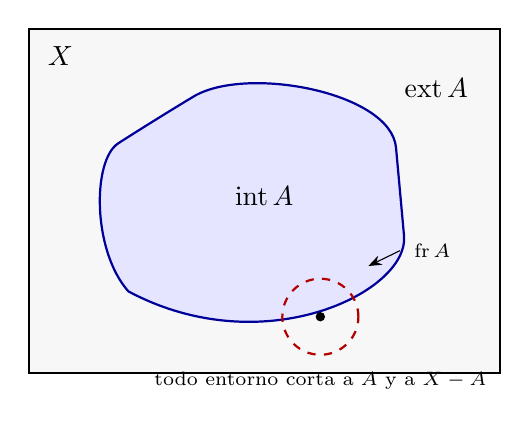
\begin{tikzpicture}[scale=1.15]
\draw[thick,fill=gray!6] (-2.6,-1.9) rectangle (2.6,1.9);
\node at (-2.25,1.6) {$X$};
\draw[abierto,rounded corners=16pt] (-1.5,-1.0) .. controls (0,-1.8) and (1.6,-1.0) .. (1.5,0.1)
 .. controls (1.4,1.2) and (-0.2,1.5) .. (-1.2,0.9) .. controls (-1.9,0.45) and (-1.9,-0.55) .. (-1.5,-1.0);
\node at (0,0.05) {$\intr A$};
\node at (1.9,1.25) {$\ext A$};
\node[right] at (1.55,-0.55) {\scriptsize $\fr A$};
\draw[->,>=Stealth,thin] (1.5,-0.55)--(1.15,-0.72);
% punto frontera con entorno
\node[pt] (b) at (0.62,-1.28) {};
\draw[red!70!black,thick,dashed] (b) circle (0.42);
\node[below] at (0.62,-1.78) {\scriptsize todo entorno corta a $A$ y a $X-A$};
\end{tikzpicture}
\figtit{Figura 4. $X$ queda partido en tres pedazos disjuntos: interior, frontera y exterior. La frontera es el conjunto de puntos ``indecisos'': por más chico que se tome el entorno, siempre se ve algo de adentro y algo de afuera.}
\end{figure}

\begin{intuicion}
$\intr A$ = ``estoy adentro con margen''; $\ext A$ = ``estoy afuera con margen''; $\fr A$ = ``estoy justo en el borde''. Un conjunto es abierto cuando no contiene nada de su borde, cerrado cuando lo contiene todo, y abierto-cerrado a la vez cuando directamente \emph{no tiene} borde (Prop.~\ref{pr:clopen}). Ojo: la frontera no siempre es una curva fina; $\fr\Q=\R$ en la recta usual, porque ningún intervalo evita a los racionales ni a los irracionales.
\end{intuicion}

\begin{ejemplo}[{Interior, clausura y frontera en la recta y en $C[-1,1]$ \fnt{GT Ej.\ 2.6.6, pp.\,30--31}}]\label{hu:ejfr}
\leavevmode\begin{enumerate}[label=(\alph*),leftmargin=2.2em,itemsep=1pt]
\item En $(\R,\tp_u)$: $\intr\Z=\emptyset$, porque todo intervalo alrededor de un entero tiene puntos no enteros; $\cl\Z=\Z$, porque el complemento $\R-\Z$ es la unión de los intervalos abiertos $(n,n+1)$; y $\fr\Z=\Z$. Así $\Z$ es cerrado y no abierto.
\item Si $a<b$, los cuatro intervalos $[a,b]$, $(a,b)$, $[a,b)$, $(a,b]$ tienen interior $(a,b)$, clausura $[a,b]$ y frontera $\{a,b\}$. Luego $[a,b]$ es cerrado y no abierto, $(a,b)$ es abierto y no cerrado, y $[a,b)$, $(a,b]$ no son ni una cosa ni la otra.
\item El \emph{conjunto de Cantor} $\mathcal C=\bigcap_{n\ge1}A_n$, con $A_1=[0,1]$ y $A_{n+1}$ obtenido de $A_n$ quitando el tercio central abierto de cada uno de sus intervalos, es cerrado: cada $A_n$ es unión finita de intervalos cerrados, y una intersección de cerrados es cerrada.
\item En $X=C[-1,1]$ con $d_\infty$, el conjunto $D$ de las funciones derivables no es cerrado: $f_n(x)=\sqrt{x^2+1/n^2}$ es derivable, y $0\le f_n(x)-|x|\le\frac1n$ da $d_\infty(f_n,|x|)\le\frac1n\to0$, pero $|x|\notin D$. De hecho $\cl D=X$: toda continua es límite uniforme de derivables (se puede demostrar, por ejemplo con el teorema de aproximación de Weierstrass; no se hace en el curso).
\end{enumerate}
\lgc{\intr\Z=\emptyset,\ \cl\Z=\fr\Z=\Z;\qquad \intr[a,b)=(a,b),\ \cl{(a,b)}=[a,b],\ \fr[a,b)=\{a,b\};\\
f_n\in D,\ d_\infty\big(f_n,|x|\big)\le\tfrac1n,\ |x|\notin D\ \Rightarrow\ D\ne\cl D.}
\end{ejemplo}

\begin{figure}[ht]
\centering
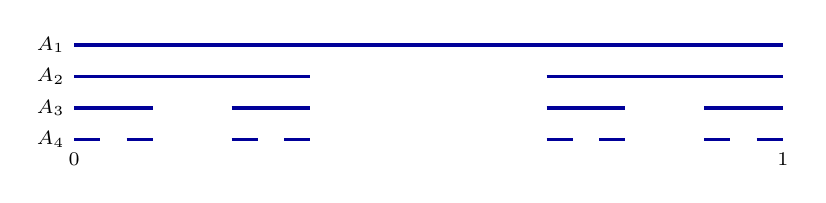
\begin{tikzpicture}[xscale=9,yscale=1]
\foreach \a/\b in {0/1}{\draw[very thick,blue!60!black] (\a,0)--(\b,0);}
\foreach \a/\b in {0/0.3333,0.6667/1}{\draw[very thick,blue!60!black] (\a,-0.4)--(\b,-0.4);}
\foreach \a/\b in {0/0.1111,0.2222/0.3333,0.6667/0.7778,0.8889/1}{\draw[very thick,blue!60!black] (\a,-0.8)--(\b,-0.8);}
\foreach \a in {0,0.0741,0.2222,0.2963,0.6667,0.7407,0.8889,0.9630}{\draw[very thick,blue!60!black] (\a,-1.2)--(\a+0.0370,-1.2);}
\node[left] at (0,0) {\scriptsize $A_1$}; \node[left] at (0,-0.4) {\scriptsize $A_2$};
\node[left] at (0,-0.8) {\scriptsize $A_3$}; \node[left] at (0,-1.2) {\scriptsize $A_4$};
\node[below] at (0,-1.25) {\scriptsize $0$}; \node[below] at (1,-1.25) {\scriptsize $1$};
\end{tikzpicture}
\figtit{Figura 5. Las primeras etapas del conjunto de Cantor. Cada $A_n$ es unión finita de intervalos cerrados; $\mathcal C$ es lo que sobrevive a todas las etapas.}
\end{figure}

\begin{proposicion}[Caracterización de los abiertos-cerrados \fnt{EJ, Top--A.11, p.\,7}]\label{pr:clopen}
Sea $(X,\tp)$ y $A\subseteq X$. Entonces $A$ es simultáneamente abierto y cerrado $\iff \fr A=\emptyset$.
\end{proposicion}

\begin{proof}
Si $A$ es abierto y cerrado, $\intr A=A=\cl A$, luego $\fr A=\cl A-\intr A=\emptyset$. Recíprocamente, si $\fr A=\emptyset$ entonces $\cl A=\intr A$; como siempre $\intr A\subseteq A\subseteq \cl A$, resulta $A=\intr A=\cl A$, o sea $A$ abierto y cerrado.
\end{proof}

\begin{definicion}[Denso \fnt{GT 2.6.7, p.\,31}]
$A$ es \emph{denso} en $(X,\tp)$ si $\cl A=X$.
\end{definicion}

\begin{proposicion}[Caracterización de la densidad \fnt{EJ, Top--A.13, p.\,7; MS Lema 3.11, p.\,42}]
Sea $(X,\tp)$ y $A\subseteq X$. Entonces $A$ es denso en $X$ $\iff$ $A\cap G\ne\emptyset$ para todo abierto $G\ne\emptyset$ $\iff$ $\intr(X-A)=\emptyset$.
\end{proposicion}

\begin{proof}
Si $A$ es denso y $G\ne\emptyset$ es abierto, tomando $x\in G$ se tiene $x\in\cl A$, luego $G\cap A\ne\emptyset$ por definición de punto adherente. Recíprocamente, si todo abierto no vacío corta a $A$, entonces todo $x\in X$ está en $\cl A$. La segunda equivalencia es la dualidad: $\cl A=X\iff X-\intr(X-A)=X$.
\end{proof}

\begin{proposicion}[La frontera de un abierto tiene interior vacío \fnt{parcial 2/10/2023, ej.\ 2b}]
Si $A\in\tp$ (o si $A$ es cerrado), entonces $\intr(\fr A)=\emptyset$.
\end{proposicion}

\begin{proof}
Sea $A$ abierto. Entonces $A\cap\fr A=\emptyset$, porque $\fr A=\cl A-\intr A=\cl A-A$. Si existiera $x\in\intr(\fr A)$, habría un abierto $G$ con $x\in G\subseteq\fr A\subseteq\cl A$; como $x\in\cl A$ y $G$ es un abierto que lo contiene, $G\cap A\ne\emptyset$, contra $\fr A\cap A=\emptyset$. Para $A$ cerrado se aplica lo anterior a $X-A$, usando $\fr A=\fr(X-A)$.
\end{proof}

\begin{observacion}[Hace falta la hipótesis]
Sin suponer $A$ abierto o cerrado el enunciado es falso: en $(\R,\tp_u)$ con $A=\Q$ es $\fr\Q=\R$ y $\intr(\fr\Q)=\R\ne\emptyset$.
\end{observacion}

\begin{definicion}[Operadores de Kuratowski \fnt{EJ, Top--D.2, p.\,8}]
$i(A)=\intr(\cl A)=(\cl A)^{\circ}$ y $c(A)=\cl{\intr A}=\cl{A^{\circ}}$.
\end{definicion}

\begin{observacion}[$i(A)$ y $c(A)$ no coinciden]
La igualdad $(\cl A)^{\circ}=\cl{A^{\circ}}$ es \emph{falsa} en general, y tampoco hay inclusión en ninguno de los dos sentidos: en $(\R,\tp_u)$, con $A=(0,1)\cup(1,2)\cup\{3\}\cup([4,5]\cap\Q)$ resulta $i(A)=(0,2)\cup(4,5)$ y $c(A)=[0,2]$, de modo que $0\in c(A)-i(A)$ y $4{,}5\in i(A)-c(A)$. Sí valen $i\circ i=i$ y $c\circ c=c$, y las inclusiones $\intr A\subseteq c(A)$ e $i(A)\subseteq\cl A$.
\end{observacion}

\begin{proposicion}[Puntos y cerrados en métricos \fnt{EJ, Top--A.12, p.\,7; GT Cor.\ 2.3.3, p.\,22}]
En $(X,d)$, todo conjunto unitario (y por ende todo conjunto finito) es cerrado; equivalentemente, $X-\{x\}$ es abierto. En particular, en un espacio métrico todos los puntos de un conjunto finito son aislados.
\end{proposicion}

\begin{proof}
Si $y\ne x$, la bola $\Bola{y}{d(x,y)}$ está contenida en $X-\{x\}$; luego $X-\{x\}$ es entorno de todos sus puntos, o sea abierto.
\end{proof}


%======================================================================
\section{Bases, subbases y comparación de topologías}\label{sec:bases}

\begin{definicion}[Comparación \fnt{EJ, Ej.\ teórico N$^\circ$2, p.\,9; Munkres \S13}]
Dadas $\tp,\tp'$ sobre $X$, se dice que $\tp'$ es \emph{más fina} que $\tp$ si $\tp\subseteq\tp'$. Es un orden \emph{parcial}: hay topologías no comparables.
\end{definicion}

\begin{definicion}[Base \emph{de} una topología dada \fnt{MS Def.\ 2.4, p.\,25}]
Sea $(X,\tp)$ un espacio topológico. $\beta\subseteq\tp$ es \emph{base de} $\tp$ si
\[
\forall U\in\tp\ \forall x\in U\ \ \exists B\in\beta:\ x\in B\subseteq U .
\]
\end{definicion}

\begin{definicion}[Base \emph{para} una topología, y topología generada \fnt{MS Def.\ 2.4, p.\,25; EJ p.\,9}]
Sea $X$ un conjunto (sin topología dada todavía). $\beta\subseteq\mathcal P(X)$ es una \emph{base} si cumple:
\begin{lista}
\item[\textbf{(B1)}] todo $x\in X$ pertenece a algún $B\in\beta$;
\item[\textbf{(B2)}] si $x\in B_1\cap B_2$ con $B_1,B_2\in\beta$, existe $B_3\in\beta$ con $x\in B_3\subseteq B_1\cap B_2$.
\end{lista}
En ese caso se define la \emph{topología generada por} $\beta$ como
\[
\tp_\beta=\{U\subseteq X:\ \forall x\in U\ \exists B\in\beta,\ x\in B\subseteq U\}.
\]
\end{definicion}

\begin{teorema}[Criterio de base \fnt{MS Teo.\ 2.3, p.\,26; EJ Ej.\ teórico N$^\circ$2.1--2.2, p.\,9}]
Sea $X$ un conjunto y $\beta\subseteq\mathcal P(X)$. Entonces $\beta$ es base de alguna topología sobre $X$ si y sólo si cumple \textbf{(B1)} y \textbf{(B2)}; en ese caso $\tp_\beta$ es efectivamente una topología, $\beta$ es base de $\tp_\beta$ en el sentido de la Definición anterior, y
\[
\tp_\beta=\Big\{\ \bigcup_{i\in I}B_i\ :\ \{B_i\}_{i\in I}\subseteq\beta\ \Big\},
\]
es decir, la topología generada coincide con la colección de todas las uniones de elementos de $\beta$ \fnt{MS Lema 2.2, p.\,25}.
\end{teorema}

\begin{proof}[Idea de la demostración]
Que $\tp_\beta$ es topología: $\emptyset$ y $X$ salen de \textbf{(B1)}; la unión es inmediata de la definición puntual; para $U_1\cap U_2$, dado $x$ en la intersección hay $B_1,B_2$ con $x\in B_i\subseteq U_i$, y \textbf{(B2)} provee $B_3\subseteq B_1\cap B_2\subseteq U_1\cap U_2$. La igualdad con las uniones: todo $U\in\tp_\beta$ es $U=\bigcup_{x\in U}B_x$; recíprocamente toda unión de básicos está en $\tp_\beta$.
\end{proof}

\begin{teorema}[Reconocer una base dentro de una topología \fnt{EJ, Ej.\ teórico N$^\circ$2.3, p.\,10; MS Lema 2.11, p.\,30; Munkres Lema 13.2}]
Sea $(X,\tp)$ y $\mathcal{C}\subseteq\tp$ una colección de abiertos tal que para todo $U\in\tp$ y todo $x\in U$ existe $C\in\mathcal{C}$ con $x\in C\subseteq U$. Entonces $\mathcal C$ es base de $\tp$.
\end{teorema}

\begin{figure}[ht]
\centering
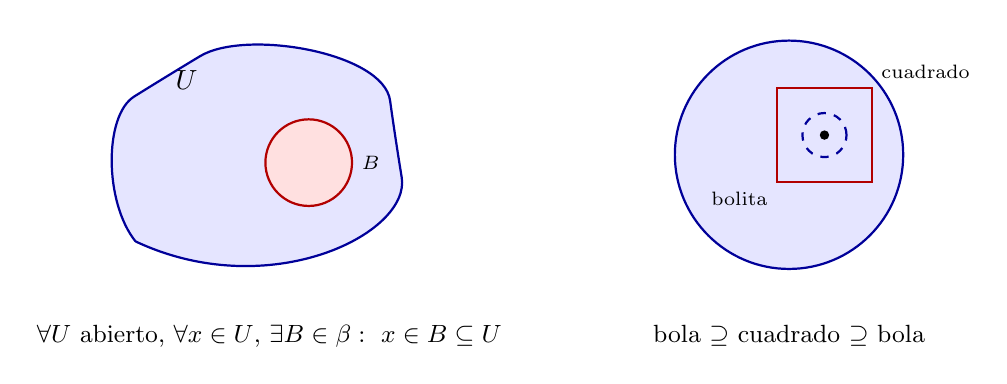
\begin{tikzpicture}[scale=1.0]
% definicion de base
\begin{scope}
\draw[abierto,rounded corners=14pt] (-1.7,-1.1) .. controls (0,-1.9) and (1.8,-1.0) .. (1.6,0.2)
 .. controls (1.45,1.3) and (-0.3,1.6) .. (-1.3,1.0) .. controls (-2.1,0.5) and (-2.1,-0.6) .. (-1.7,-1.1);
\node at (-1.05,0.95) {$U$};
\node[pt] (p) at (0.5,-0.1) {}; \node[below] at (0.5,-0.18) {\scriptsize $x$};
\draw[red!70!black,thick,fill=red!12] (p) circle (0.55);
\node[right] at (1.05,-0.1) {\scriptsize $B$};
\node at (0,-2.3) {\small $\forall U$ abierto, $\forall x\in U$, $\exists B\in\beta:\ x\in B\subseteq U$};
\end{scope}
% bolas y cuadrados
\begin{scope}[xshift=6.6cm]
\draw[abierto] (0,0) circle (1.45);
\node[pt] (q) at (0.45,0.25) {};
\draw[red!70!black,thick] (-0.15,-0.35) rectangle (1.05,0.85);
\draw[blue!60!black,thick,dashed] (q) circle (0.28);
\node[above right] at (1.05,0.85) {\scriptsize cuadrado};
\node[below left] at (-0.15,-0.35) {\scriptsize bolita};
\node at (0,-2.3) {\small bola $\supseteq$ cuadrado $\supseteq$ bola};
\end{scope}
\end{tikzpicture}
\figtit{Figura 6. Izquierda: qué pide ser base. Derecha: por qué bolas y cuadrados generan la \emph{misma} topología en $\R^2$ --- cada básico de un tipo contiene, alrededor de cada uno de sus puntos, un básico del otro tipo. Ese es literalmente el criterio de comparación (Teo.~\ref{th:compbase}) aplicado en las dos direcciones.}
\end{figure}

\begin{intuicion}
Una base es una ``lista de piezas de repuesto'': en lugar de describir todos los abiertos, se describen unos pocos con los que se pueden armar todos los demás por unión. Como en el armado solo importa poder \emph{encajar} una pieza chica alrededor de cada punto, dos listas de piezas de formas totalmente distintas pueden armar exactamente los mismos objetos.
\end{intuicion}

\begin{ejemplo}
Con este criterio se ve de inmediato que en $\R^2$ las bolas euclídeas, los cuadrados abiertos y los rombos abiertos son todos bases de la \emph{misma} topología usual: a diferencia del álgebra lineal, las bases no son únicas ni tienen ``dimensión'' \fnt{EJ p.\,10}.
\end{ejemplo}

\begin{teorema}[Comparación mediante bases \fnt{MS Teo.\ 2.4 y Cor.\ 2.5, p.\,27; EJ Ej.\ teórico N$^\circ$2.4, p.\,10}]\label{th:compbase}
Sean $\beta$ y $\beta'$ bases de $\tp$ y $\tp'$. Entonces $\tp\subseteq\tp'$ ($\tp'$ más fina) si y sólo si
\[
\forall x\in X,\ \forall B\in\beta \text{ con } x\in B,\ \exists B'\in\beta' \text{ tal que } x\in B'\subseteq B .
\]
En consecuencia $\tp=\tp'$ si y sólo si vale la condición en ambas direcciones.
\end{teorema}

\begin{proof}
($\Rightarrow$) Si $B\in\beta\subseteq\tp\subseteq\tp'$ y $x\in B$, como $\beta'$ es base de $\tp'$ existe $B'\in\beta'$ con $x\in B'\subseteq B$. ($\Leftarrow$) Sea $U\in\tp$ y $x\in U$; hay $B\in\beta$ con $x\in B\subseteq U$ y, por hipótesis, $B'\in\beta'$ con $x\in B'\subseteq B\subseteq U$; luego $U\in\tp'$.
\end{proof}

\begin{definicion}[Subbase \fnt{MS Lema 2.6, p.\,27}]
$\sigma\subseteq\mathcal P(X)$ es una \emph{subbase} si $\bigcup_{S\in\sigma}S=X$. La \emph{topología generada por la subbase} $\sigma$ es la generada por la base del lema siguiente.
\end{definicion}

\begin{lema}[Una subbase genera una base \fnt{MS Lema 2.6, p.\,27; EJ Ej.\ teórico N$^\circ$2.6, p.\,10}]
Si $\sigma$ es una subbase, la colección de \emph{intersecciones finitas} de elementos de $\sigma$ cumple \textbf{(B1)} y \textbf{(B2)}, luego es base de una topología, y esa topología es la menos fina que contiene a $\sigma$.
\lgc{\sigma\ \text{subbase}\ \Rightarrow\ \Big\{\bigcap_{k=1}^{n}S_k:\ S_k\in\sigma,\ n\in\N\Big\}\ \text{es base};\\
\tp_\sigma=\min\{\tp:\ \sigma\subseteq\tp\}.}
\end{lema}


\begin{ejemplo}[Sorgenfrey \fnt{MS Ejemplos 2.4(7), p.\,26}]
$\beta_{sor}=\{[a,b): a<b\}$ genera la recta de Sorgenfrey, también estrictamente más fina que la usual, y en la que cada $[a,b)$ es a la vez abierto y cerrado.
\end{ejemplo}

\subsection{Entornos y bases de entornos}

\begin{teorema}[Axiomas de entorno \fnt{MS Teo.\ 2.7, p.\,28}]
Sea $(X,\tp)$ y $x\in X$. El sistema de entornos $\mathcal N_x=\{N\subseteq X:\ x\in\intr N\}$ verifica:
\begin{lista}
\item (N1) si $N\in\mathcal N_x$ entonces $x\in N$;
\item (N2) si $N\in\mathcal N_x$ y $N\subseteq M$ entonces $M\in\mathcal N_x$;
\item (N3) $\mathcal N_x$ es cerrado por intersecciones finitas;
\item (N4) si $N\in\mathcal N_x$, existe $M\in\mathcal N_x$ con $M\subseteq N$ tal que $N\in\mathcal N_y$ para todo $y\in M$.
\end{lista}
\end{teorema}

\begin{definicion}[Base local \fnt{MS Teo.\ 2.8, p.\,29}]
$\mathcal B_x\subseteq\mathcal N_x$ es \emph{base de entornos} (o \emph{base local}) en $x$ si todo entorno de $x$ contiene algún elemento de $\mathcal B_x$.
\lgc{\mathcal B_x\ \text{base local en } x\iff \forall N\in\mathcal N_x\ \exists B\in\mathcal B_x:\ B\subseteq N.}
\end{definicion}

\begin{proposicion}[Bases locales que siempre sirven \fnt{MS Lema 2.9, p.\,30}]
Sea $(X,\tp)$ y $x\in X$:
\begin{lista}
\item la familia de los entornos \emph{abiertos} de $x$ es base local en $x$, en cualquier espacio topológico;
\item en un espacio métrico, $\{\Bola{x}{1/n}: n\in\N\}$ es base local en $x$ (base local \emph{numerable}).
\end{lista}
\end{proposicion}


\begin{teorema}[La familia de bolas es base \fnt{MS Teo.\ 2.14, p.\,32}]
En $(X,d)$, $\{\Bola{x}{r}: x\in X, r>0\}$ es base de una topología sobre $X$, llamada \emph{topología métrica} $\tp_d$. Un espacio $(X,\tp)$ es \emph{metrizable} si existe $d$ con $\tp=\tp_d$.
\end{teorema}

%======================================================================
\section{Axiomas de separación $T_0$, $T_1$, $T_2$}\label{sec:sep}

\begin{definicion}[\fnt{EJ, Ejercicios teóricos $T_0,T_1$, Hausdorff, p.\,11; GT 2.5.3, p.\,27}]
Sea $(X,\tp)$ y $x\ne y$ en $X$.
\begin{itemize}[leftmargin=1.4em,itemsep=1pt]
\item $X$ es $T_0$ si existe un abierto que contiene a uno de los dos y no al otro.
\item $X$ es $T_1$ si existe un abierto $U$ con $x\in U$, $y\notin U$ \emph{y} un abierto $V$ con $y\in V$, $x\notin V$.
\item $X$ es $T_2$ (\emph{Hausdorff}) si existen abiertos disjuntos $U\ni x$, $V\ni y$.
\end{itemize}
\lgc{T_0:\ \forall x\ne y\ \exists U\in\tp:\ (x\in U\wedge y\notin U)\vee(y\in U\wedge x\notin U);\\
T_1:\ \forall x\ne y\ \exists U,V\in\tp:\ (x\in U\wedge y\notin U)\wedge(y\in V\wedge x\notin V);\\
T_2:\ \forall x\ne y\ \exists U,V\in\tp:\ x\in U\ \wedge\ y\in V\ \wedge\ U\cap V=\emptyset.}
\end{definicion}

\begin{figure}[ht]
\centering
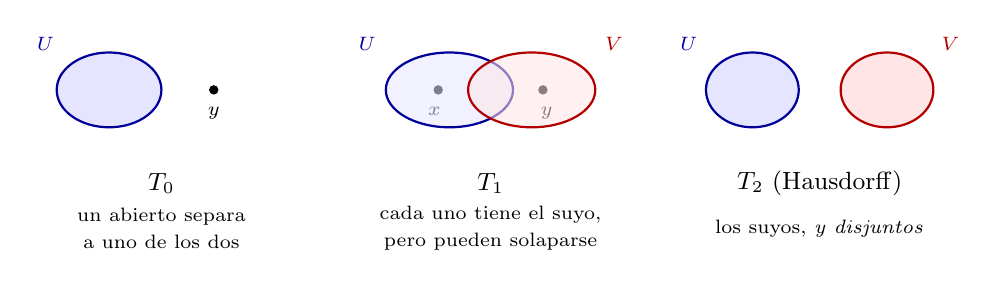
\begin{tikzpicture}[scale=0.95]
% T0
\begin{scope}
\node[pt] (a) at (-0.5,0) {}; \node[below] at (-0.5,-0.1) {\scriptsize $x$};
\node[pt] (b) at (0.9,0) {}; \node[below] at (0.9,-0.1) {\scriptsize $y$};
\draw[blue!60!black,thick,fill=blue!10] (-0.5,0) ellipse (0.7 and 0.5);
\node[blue!60!black] at (-1.35,0.62) {\scriptsize $U$};
\node at (0.2,-1.25) {\small $T_0$};
\node[align=center] at (0.2,-1.85) {\scriptsize un abierto separa\\[-2pt]\scriptsize a uno de los dos};
\end{scope}
% T1
\begin{scope}[xshift=4.4cm]
\node[pt] (a) at (-0.5,0) {}; \node[below] at (-0.55,-0.1) {\scriptsize $x$};
\node[pt] (b) at (0.9,0) {}; \node[below] at (0.95,-0.1) {\scriptsize $y$};
\draw[blue!60!black,thick,fill=blue!10,fill opacity=0.55] (-0.35,0) ellipse (0.85 and 0.5);
\draw[red!70!black,thick,fill=red!10,fill opacity=0.55] (0.75,0) ellipse (0.85 and 0.5);
\node[blue!60!black] at (-1.45,0.62) {\scriptsize $U$};
\node[red!70!black] at (1.85,0.62) {\scriptsize $V$};
\node at (0.2,-1.25) {\small $T_1$};
\node[align=center] at (0.2,-1.85) {\scriptsize cada uno tiene el suyo,\\[-2pt]\scriptsize pero pueden solaparse};
\end{scope}
% T2
\begin{scope}[xshift=8.8cm]
\node[pt] (a) at (-0.7,0) {}; \node[below] at (-0.75,-0.1) {\scriptsize $x$};
\node[pt] (b) at (1.1,0) {}; \node[below] at (1.15,-0.1) {\scriptsize $y$};
\draw[blue!60!black,thick,fill=blue!10] (-0.7,0) ellipse (0.62 and 0.5);
\draw[red!70!black,thick,fill=red!10] (1.1,0) ellipse (0.62 and 0.5);
\node[blue!60!black] at (-1.55,0.62) {\scriptsize $U$};
\node[red!70!black] at (1.95,0.62) {\scriptsize $V$};
\node at (0.2,-1.25) {\small $T_2$ (Hausdorff)};
\node[align=center] at (0.2,-1.85) {\scriptsize los suyos, \emph{y disjuntos}};
\end{scope}
\end{tikzpicture}
\figtit{Figura 7. Los tres niveles de separación. Cada uno pide un poco más que el anterior: $T_2\Rightarrow T_1\Rightarrow T_0$.}
\end{figure}

\begin{intuicion}
La pregunta de fondo es ``¿cuánto puede la topología distinguir dos puntos distintos?''. En la cofinita se pueden aislar puntos ($T_1$) pero los abiertos son tan enormes que dos cualesquiera se cortan, así que no hay $T_2$; ahí es donde se rompe la unicidad del límite de una sucesión. En un espacio métrico las bolas de radio $d(x,y)/2$ hacen el trabajo automáticamente, y por eso todo métrico es $T_2$.
\end{intuicion}

\begin{proposicion}[Jerarquía \fnt{EJ, Ej.\ teórico 3, p.\,11}]
Para todo espacio topológico $(X,\tp)$: $T_2\Rightarrow T_1\Rightarrow T_0$, y ninguna recíproca vale.
\end{proposicion}

\begin{ejemplo}[Contraejemplos de las recíprocas]
\begin{itemize}[leftmargin=1.4em,itemsep=1pt]
\item $T_1$ pero no $T_2$: $(X,\tp_{cof})$ con $X$ infinito. Los cerrados son los finitos, luego los puntos son cerrados y el espacio es $T_1$; pero dos abiertos no vacíos cualesquiera se cortan (sus complementos son finitos y $X$ es infinito), luego no es $T_2$.
\item $T_0$ pero no $T_1$: el espacio de Sierpi\'nski $X=\{a,b\}$, $\tp=\{\emptyset,X,\{a\}\}$; o el espacio del ejercicio 2 de la guía, $X=\{a,b,c\}$ con $\tp=\{\emptyset,X,\{a,b\},\{a\}\}$, en el cual $\{a\}$ no es cerrado \fnt{EJ, Ej.\ teórico 2 y 3d, p.\,11}.
\end{itemize}
\end{ejemplo}

\begin{teorema}[Caracterización de $T_1$ \fnt{EJ, Ej.\ teórico 4, p.\,11}]
Sea $(X,\tp)$ un espacio topológico. Entonces $(X,\tp)$ es $T_1$ $\iff$ $\{x\}$ es cerrado para todo $x\in X$.
\end{teorema}

\begin{proof}
$\{x\}$ es cerrado $\iff X-\{x\}$ es abierto $\iff$ $X-\{x\}$ es entorno de todos sus puntos $\iff$ para cada $y\ne x$ existe un abierto $V$ con $y\in V\subseteq X-\{x\}$, es decir $y\in V$ y $x\notin V$. Esto, para todo par $x\ne y$, es exactamente $T_1$.
\end{proof}

\begin{teorema}[Todo métrico es Hausdorff \fnt{GT 1.1.26, p.\,11; MS Teo.\ 2.13, p.\,32}]
Todo espacio métrico es $T_2$ (y por lo tanto $T_1$ y $T_0$). En consecuencia, cualquier espacio no Hausdorff no es metrizable.
\end{teorema}

%======================================================================
\section{Sucesiones y convergencia}\label{sec:suc}

\begin{definicion}[\fnt{GT 2.5.1, p.\,26}]
$\{x_n\}_{n\ge1}$ \emph{converge} a $x_0$ en $(X,\tp)$ si para todo abierto $G$ con $x_0\in G$ existe $n_0$ tal que $x_n\in G$ para todo $n\ge n_0$. En un espacio métrico esto equivale a $d(x_n,x_0)\to 0$.
\lgc{x_n\to x_0\iff \forall G\in\tp\ \big(x_0\in G\Rightarrow \exists n_0\ \forall n\ge n_0:\ x_n\in G\big).}
\end{definicion}

\begin{teorema}[Unicidad del límite \fnt{GT 2.5.2, p.\,26; GT Nota 2.5.4, p.\,27; EJ Ej.\ teórico 5, p.\,11}]
En un espacio de Hausdorff (en particular, en todo espacio métrico), toda sucesión convergente tiene un único límite.
\lgc{X\ \text{es } T_2\ \Rightarrow\ \big(x_n\to x\ \wedge\ x_n\to y\ \Rightarrow\ x=y\big).}
\end{teorema}

\begin{proof}
Si $x_n\to x$ y $x_n\to y$ con $x\ne y$, tomo abiertos disjuntos $U\ni x$, $V\ni y$. Existen $n_1,n_2$ con $x_n\in U$ para $n\ge n_1$ y $x_n\in V$ para $n\ge n_2$; para $n\ge\max\{n_1,n_2\}$ resulta $x_n\in U\cap V=\emptyset$, absurdo.
\end{proof}

\begin{ejemplo}[Sin Hausdorff, infinitos límites \fnt{GT Ej.\ 2.5.5, p.\,27}]\label{hu:inflim}
En $\R^2$ con la seudodistancia $d\big((x,y),(x',y')\big)=|x-x'|$ (Ej.~\ref{hu:seudoR2}), la sucesión $(1/n,0)$ converge a \emph{todos} los puntos $(0,y)$ del eje vertical: si $G$ es abierto y $(0,y)\in G$, hay $\varepsilon>0$ con $\Bola{(0,y)}{\varepsilon}\subseteq G$, y para $n\ge n_0>1/\varepsilon$ se tiene $d\big((1/n,0),(0,y)\big)=1/n<\varepsilon$. Por el teorema anterior (contrarrecíproco), el espacio no es de Hausdorff.
\lgc{\forall y\in\R:\ (1/n,0)\to(0,y)\ \text{en } (\R^2,\tp_d)\ \Rightarrow\ (\R^2,\tp_d)\ \text{no es } T_2.}
\end{ejemplo}

\begin{figure}[ht]
\centering
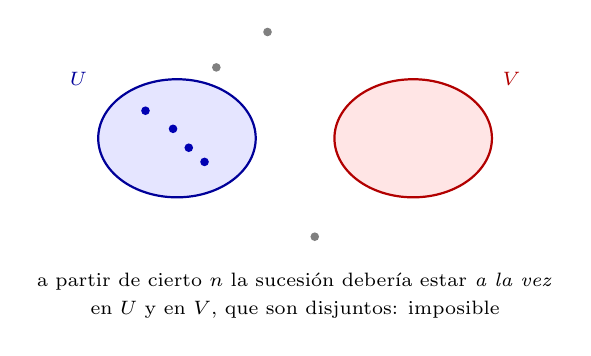
\begin{tikzpicture}[scale=1.0]
\node[pt] (x) at (-1.5,0) {}; \node[below] at (-1.5,-0.12) {\scriptsize $x$};
\node[pt] (y) at (1.5,0) {}; \node[below] at (1.5,-0.12) {\scriptsize $y$};
\draw[blue!60!black,thick,fill=blue!10] (-1.5,0) ellipse (1.0 and 0.75);
\draw[red!70!black,thick,fill=red!10] (1.5,0) ellipse (1.0 and 0.75);
\node[blue!60!black] at (-2.75,0.75) {\scriptsize $U$};
\node[red!70!black] at (2.75,0.75) {\scriptsize $V$};
\foreach \x/\y in {-0.35/1.35,0.25/-1.25,-1.0/0.9}{
  \node[pt,fill=gray,inner sep=1.1pt] at (\x,\y) {};}
\foreach \x/\y in {-1.9/0.35,-1.15/-0.3,-1.55/0.12,-1.35/-0.12}{
  \node[pt,fill=blue!70!black,inner sep=1.1pt] at (\x,\y) {};}
\node[align=center] at (0,-2.0) {\scriptsize a partir de cierto $n$ la sucesión debería estar \emph{a la vez}\\[-2pt]\scriptsize en $U$ y en $V$, que son disjuntos: imposible};
\end{tikzpicture}
\figtit{Figura 8. Por qué en un Hausdorff el límite es único. Si el espacio no separa (indiscreta, cofinita), esta contradicción desaparece y una misma sucesión puede converger a todos lados.}
\end{figure}


\begin{teorema}[Clausura por sucesiones (solo en métricos) \fnt{GT 2.5.6 y Cor.\ 2.5.7, p.\,28; MS Teo.\ 4.14, p.\,55}]\label{th:clsuc}
Sea $(X,d)$ métrico y $A\subseteq X$. Entonces $x\in\cl A$ $\iff$ existe $\{a_n\}\subseteq A$ con $a_n\to x$. En consecuencia, $A$ es cerrado $\iff$ $A$ contiene el límite de toda sucesión de puntos de $A$ que converja en $X$.
\lgc{(X,d):\quad x\in\cl A\iff \exists\{a_n\}_{n\ge1}\subseteq A:\ a_n\to x;\\
A\ \text{cerrado}\iff \forall\{a_n\}\subseteq A\ \big(a_n\to x\Rightarrow x\in A\big).}
\end{teorema}

\begin{observacion}
La equivalencia usa de manera esencial la base local numerable $\{\Bola{x}{1/n}\}$ y por eso \emph{no} se generaliza a espacios topológicos arbitrarios. Es la razón por la que en topología general se reemplazan las sucesiones por redes o filtros.
\end{observacion}

%======================================================================
\section{Continuidad}\label{sec:cont}

\subsection{Continuidad en un punto}\label{sec:contpt}

\begin{definicion}[Continuidad en un punto \fnt{MS Def.\ 4.1, p.\,51}]
$f:(X,\tp_X)\to(Y,\tp_Y)$ es \emph{continua en $a\in X$} si para todo entorno $M$ de $f(a)$ existe un entorno $N$ de $a$ con $f(N)\subseteq M$. Equivalentemente: $f^{-1}(M)\in\mathcal N_a$ para todo $M\in\mathcal N_{f(a)}$. $f$ es \emph{continua en $A$} si lo es en cada punto de $A$, y \emph{continua} (a secas) si lo es en todo $X$.
\lgc{f\ \text{continua en } a\iff \forall M\in\mathcal N_{f(a)}\ \exists N\in\mathcal N_a:\ f(N)\subseteq M
\iff \forall M\in\mathcal N_{f(a)}:\ f^{-1}(M)\in\mathcal N_a.}
\end{definicion}

\begin{proposicion}[Versión $\varepsilon$--$\delta$ local \fnt{MS Def.\ 4.1, p.\,51 (con la base local de bolas); GT 2.8.4, p.\,36}]
Entre espacios métricos, $f:(X,d)\to(Y,\rho)$ es continua en $a$ $\iff$
\[
\forall \varepsilon>0\ \exists \delta>0:\quad d(x,a)<\delta \ \Longrightarrow\ \rho(f(x),f(a))<\varepsilon,
\]
es decir $f(\Bola{a}{\delta})\subseteq \Bola{f(a)}{\varepsilon}$. Y $f$ es continua en $a$ $\iff$ para toda sucesión $x_n\to a$ vale $f(x_n)\to f(a)$ (continuidad secuencial \emph{en $a$}).
\end{proposicion}

\begin{observacion}[Alcanza con entornos básicos]
Si $\mathcal B_{f(a)}$ es una base local en $f(a)$, basta verificar la condición para los $M\in\mathcal B_{f(a)}$: cualquier otro entorno contiene uno de ellos, y la preimagen de un conjunto mayor sigue siendo entorno. Por eso en un métrico alcanza con las bolas, y hacia $\R$ alcanza con los intervalos.
\end{observacion}

\begin{observacion}[Cómo se prueba una discontinuidad]
Negando la definición: $f$ \emph{no} es continua en $a$ si existe $\varepsilon_0>0$ tal que \emph{toda} bola $\Bola{a}{\delta}$ contiene algún $x$ con $\rho(f(x),f(a))\ge\varepsilon_0$. En la práctica lo más rápido es exhibir dos sucesiones $x_n\to a$ e $y_n\to a$ con $\lim f(x_n)\ne \lim f(y_n)$.
\end{observacion}


\begin{figure}[ht]
\centering
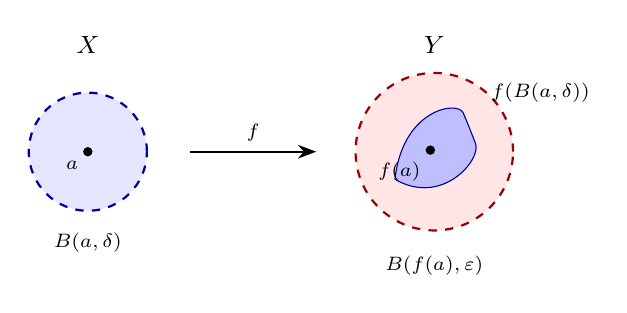
\begin{tikzpicture}[scale=1.0]
% epsilon-delta
\begin{scope}
\draw[abierto,dashed] (0,0) circle (0.75);
\node[pt] at (0,0) {}; \node[below left] at (0,0) {\scriptsize $a$};
\node at (0,-1.15) {\scriptsize $B(a,\delta)$};
\node at (0,1.35) {\small $X$};
\end{scope}
\draw[->,>=Stealth,thick] (1.3,0)--(2.9,0) node[midway,above]{\scriptsize $f$};
\begin{scope}[xshift=4.4cm]
\draw[cerrado,dashed] (0,0) circle (1.0);
\draw[fill=blue!25,draw=blue!60!black,rounded corners=6pt]
  (-0.5,-0.35) .. controls (0.1,-0.7) and (0.6,-0.1) .. (0.45,0.3)
  .. controls (0.3,0.65) and (-0.4,0.55) .. (-0.5,-0.35);
\node[pt] at (-0.05,0.02) {}; \node[below left] at (-0.05,0.0) {\scriptsize $f(a)$};
\node at (0,-1.45) {\scriptsize $B(f(a),\varepsilon)$};
\node at (1.35,0.75) {\scriptsize $f(B(a,\delta))$};
\node at (0,1.35) {\small $Y$};
\end{scope}
\end{tikzpicture}
\figtit{Figura 9. Continuidad en $a$: dado el objetivo $\varepsilon$ (la bola de llegada), hay una tolerancia $\delta$ (la bola de salida) cuya imagen entra completa. Primero se fija $\varepsilon$, después se busca $\delta$ --- nunca al revés.}
\end{figure}

\begin{intuicion}
La versión topológica ``$f^{-1}(\text{abierto})$ es abierto'' es la misma idea sin números: un abierto es un conjunto que contiene un margen alrededor de cada punto suyo, y la continuidad dice que ese margen se puede \emph{tirar hacia atrás} por $f$. Por eso se trabaja con preimágenes y no con imágenes: la preimagen respeta uniones, intersecciones y complementos; la imagen, no.
\end{intuicion}

\subsection{Continuidad global}\label{sec:contglob}

\begin{definicion}[Continuidad \fnt{GT 2.8.1, p.\,34}]
$f:(X,\tp)\to(Y,\tp')$ es \emph{continua} si $f(\cl A)\subseteq \cl{f(A)}$ para todo $A\subseteq X$ (``la imagen de lo adherido queda adherida'').
\end{definicion}

\begin{teorema}[Caracterización por abiertos y cerrados \fnt{GT 2.8.2, p.\,34; MS Prop.\ 4.1, p.\,51}]\label{th:contab}
Sea $f:(X,\tp)\to(Y,\tp')$ una función cualquiera y sea $\beta'$ una base (o una subbase) fijada de $\tp'$. Son equivalentes:
\begin{enumerate}[label=(\arabic*),leftmargin=2.2em,itemsep=0pt]
\item $f$ es continua, es decir $f(\cl A)\subseteq\cl{f(A)}$ para todo $A\subseteq X$;
\item $f^{-1}(F)$ es cerrado en $X$, para todo cerrado $F$ de $Y$;
\item $f^{-1}(G)$ es abierto en $X$, para todo abierto $G$ de $Y$;
\item $f^{-1}(B)$ es abierto en $X$, para todo $B\in\beta'$ (alcanza con los \emph{básicos}, no hace falta recorrer todos los abiertos de $Y$);
\item $f^{-1}(M)$ es entorno de $x$, para cada $x\in X$ y cada entorno $M\in\mathcal N_{f(x)}$;
\item $f^{-1}(\cl B)\supseteq \cl{f^{-1}(B)}$ y $f^{-1}(\intr B)\subseteq \intr\big(f^{-1}(B)\big)$, para todo $B\subseteq Y$.
\end{enumerate}
\end{teorema}

\begin{proof}[Demostración de $(1)\Rightarrow(2)\Rightarrow(3)\Rightarrow(1)$]
$(1)\Rightarrow(2)$: sea $F$ cerrado y $A=f^{-1}(F)$. Por (1), $f(\cl{A})\subseteq\cl{f(A)}\subseteq \cl F=F$, luego $\cl A\subseteq f^{-1}(F)=A$; como siempre $A\subseteq\cl A$, resulta $A$ cerrado.
$(2)\Rightarrow(3)$: $f^{-1}(Y-G)=X-f^{-1}(G)$.
$(3)\Rightarrow(1)$: sea $y\in f(\cl A)$, digamos $y=f(x)$ con $x\in\cl A$, y sea $G$ abierto con $y\in G$. Entonces $f^{-1}(G)$ es abierto y contiene a $x\in \cl A$, luego $f^{-1}(G)\cap A\ne\emptyset$; tomando $a$ en esa intersección, $f(a)\in G\cap f(A)$. Por lo tanto $y\in\cl{f(A)}$.
\end{proof}

\begin{observacion}
El punto (4) es el que más se usa en la práctica: para probar continuidad hacia $\R$ basta ver que las preimágenes de $(a,b)$ (o incluso de $(a,\infty)$ y $(-\infty,b)$, que forman subbase) son abiertas.
\end{observacion}

\begin{teorema}[Caracterización $\varepsilon$--$\delta$ \fnt{GT 2.8.4, p.\,36}]
Sean $(X,d)$ e $(Y,d')$ espacios métricos y $f:X\to Y$. Entonces $f$ es continua $\iff$ para todo $x\in X$ y todo $\varepsilon>0$ existe $\delta>0$ con $f(\Bola{x}{\delta})\subseteq \Bola{f(x)}{\varepsilon}$.
\end{teorema}

\begin{teorema}[Caracterización por sucesiones \fnt{GT 2.8.5, p.\,36; MS Teo.\ 4.15, p.\,56}]\label{th:seq}
Entre espacios métricos, $f$ es continua $\iff$ $x_n\to x_0$ implica $f(x_n)\to f(x_0)$ (continuidad secuencial).
\end{teorema}

\begin{observacion}[Dónde vale cada dirección \fnt{clase 8, balance de la Prop.\ 2.8.5}]
La dirección $\Rightarrow$ vale en \emph{cualquier} espacio topológico: dado $G$ abierto con $f(x_0)\in G$, la preimagen $f^{-1}(G)$ es un abierto que contiene a $x_0$, la cola de $\{x_n\}$ entra ahí, y por definición de preimagen la cola de $\{f(x_n)\}$ entra en $G$. La dirección $\Leftarrow$ es la que necesita métrica, porque usa la caracterización de la clausura por sucesiones (Teo.~\ref{th:clsuc}) para \emph{fabricar} una sucesión $a_n\to x$ dentro de $A$; esa caracterización solo vale en (seudo)métricos. Moraleja: en un espacio topológico general, ser secuencialmente continua no implica ser continua.
\end{observacion}

\begin{definicion}[Inclusión, restricción y correstricción \fnt{GT 2.8.6d y 2.8.7, pp.\,37--38; TS Obs.\ 3.1.4}]
Sea $f:X\to Y$ una función y $A\subseteq X$.
\begin{lista}
\item La \emph{inclusión} de $A$ en $X$ es la función $i:A\to X$ dada por $i(a)=a$ para todo $a\in A$. Es la identidad de $X$ mirada sólo sobre $A$: no mueve ningún punto, lo único que cambia es el conjunto de partida. Su preimagen es la traza: $i^{-1}(U)=U\cap A$ para todo $U\subseteq X$.
\item La \emph{restricción} de $f$ a $A$ es $f|_A:A\to Y$, $f|_A(a)=f(a)$. Restringir es componer con la inclusión: $f|_A=f\circ i$.
\item Si $f(X)\subseteq B\subseteq Y$, la \emph{correstricción} de $f$ a $B$ es $f|^{B}:X\to B$ con la misma fórmula, cambiando sólo el codominio. El caso $B=f(X)$ es la \emph{correstricción a la imagen}, que se nota $\widetilde f:X\to f(X)$ y es sobreyectiva por construcción.
\end{lista}
Cuando se habla de continuidad de $i$, de $f|_A$ o de $\widetilde f$, el subconjunto lleva siempre la topología relativa (\S\ref{sec:sub}).
\lgc{i:A\to X,\ i(a)=a\ \ \forall a\in A;\qquad i^{-1}(U)=U\cap A;\qquad f|_A=f\circ i;\\
f|^{B}:X\to B\ \text{con } f|^{B}(x)=f(x);\qquad \widetilde f=f|^{f(X)}.}
\end{definicion}

\begin{intuicion}
Las tres operaciones no tocan la fórmula de la función: cambian el dominio, el codominio, o ambos. Eso es justo lo que las vuelve delicadas en topología, porque ``abierto'' depende del espacio en el que se mira: una función puede ser continua como $f:X\to Y$ y su correstricción serlo por razones distintas. La identidad $i^{-1}(U)=U\cap A$ es la que conecta todo esto con la topología de subespacio: pedir que $i$ sea continua es pedir que las trazas $U\cap A$ sean abiertas en $A$.
\end{intuicion}

\begin{proposicion}[Propiedades generales \fnt{GT 2.8.6, p.\,37; MS Prop.\ 4.2, p.\,52}]
Entre espacios topológicos $(X,\tp)$, $(Y,\tp')$, $(Z,\tp'')$ y para $A\subseteq X$ con la topología relativa $\tp_A$:
\begin{lista}
\item las constantes son continuas;
\item la identidad es continua;
\item la composición de continuas es continua;
\item la restricción de una continua a un subespacio es continua;
\item en particular, la inclusión $i:(A,\tp_A)\to(X,\tp)$ es continua.
\end{lista}
\end{proposicion}

\begin{proposicion}[Criterio de Hausdorff de comparación \fnt{MS Prop.\ 4.3, p.\,52; [AP] Ej.\ 2.8.8 (clase 8)}]\label{pr:idcont}
Sean $\tp_1$ y $\tp_2$ dos topologías sobre el \emph{mismo} conjunto $X$, y sea $1_X$ la identidad. Entonces $\tp_2\subseteq\tp_1\iff 1_X:(X,\tp_1)\to(X,\tp_2)$ es continua. (Toda comparación de topologías puede leerse como una afirmación de continuidad.)
\end{proposicion}

\begin{proof}[Demostración, en una línea]
La identidad no mueve los puntos, así que $1_X^{-1}(G)=G$ para todo $G\subseteq X$. Entonces ``$1_X$ continua'' significa ``todo $G\in\tp_2$ está en $\tp_1$'', que es $\tp_2\subseteq\tp_1$.
\end{proof}

\begin{ejemplo}[La identidad entre topologías concretas \fnt{[AP] Ejs.\ 2.8.8 y 2.8.10 (clase 8)}]\label{ej:iddisc}
\begin{itemize}[leftmargin=1.4em,itemsep=1pt]
\item $1_\R:(\R,\tp_u)\to(\R,\tp_{dis})$ \emph{no} es continua: $\tp_{dis}\not\subseteq\tp_u$. Vía sucesiones (Teo.~\ref{th:seq}): $\tfrac1n\to0$ en la euclídea, pero $B_{d_D}(0,\varepsilon)=\{0\}$ es un abierto que contiene al límite y a ningún término, así que $1_\R(\tfrac1n)\not\to 0$ en la discreta.
\item $1_\R:(\R,\tp_{dis})\to(\R,\tp_u)$ \emph{sí} es continua, porque $\tp_u\subseteq\tp_{dis}$. Conclusión: la identidad es biyectiva y continua en un sentido, pero no es homeomorfismo --- otro contraejemplo válido para Continuidad--B.3.
\item $1_{\R^2}:(\R^2,d_e)\to(\R^2,d_{\text{taxi}})$ y su inversa son ambas continuas, porque las dos métricas dan la misma topología (Prop.~\ref{pr:equiv}). Acá la identidad \emph{sí} es homeomorfismo, con distancias distintas en salida y llegada.
\end{itemize}
\end{ejemplo}

\subsection{Álgebra de funciones continuas a valores reales}\label{sec:alg}

\begin{proposicion}[Continuidad hacia $\R^n$ \fnt{GT 2.8.11--2.8.12, pp.\,38--39} \fnt{demostrada en general en el Teo.~\ref{th:contprod}}]\label{pr:coord}
Las proyecciones $p_i:(\R^n,\text{eucl.})\to(\R,\text{eucl.})$ son continuas, y $f:(X,\tp)\to(\R^n,\text{eucl.})$ es continua $\iff$ $p_i\circ f$ es continua para todo $i$. Esto reduce ejercicios como $f(x,y)=(x,x+y,x-y)$ o $f(x,y,z)=(x+y+z,xyz)$ a la continuidad de funciones a valores reales \fnt{EJ, Continuidad--A.4, p.\,12}.
\lgc{p_i:(\R^n,\text{eucl.})\to(\R,\text{eucl.})\ \text{continua};\\
f:(X,\tp)\to\R^n\ \text{continua}\iff \forall i\in\{1,\dots,n\}:\ p_i\circ f\ \text{continua}.}
\end{proposicion}

\begin{teorema}[Operaciones \fnt{consecuencia estándar de GT 2.8.6 y 2.8.12, pp.\,37--39; MS \S4.1, p.\,51}]
Sean $f,g:(X,\tp)\to(\R,\tp_u)$ continuas y $\lambda\in\R$. Entonces son continuas:
\[
f+g,\qquad \lambda f,\qquad f\cdot g,\qquad |f|,\qquad \max\{f,g\},\qquad \min\{f,g\},
\]
y $f/g$ en el abierto $\{x: g(x)\ne0\}$.
\end{teorema}

\begin{proof}[Esquema]
La ruta corta usa dos ingredientes ya disponibles: (i) $F=(f,g):X\to\R^2$ es continua porque sus dos coordenadas lo son (Prop.~\ref{pr:coord}); (ii) las operaciones $s(u,v)=u+v$ y $m(u,v)=uv$ son continuas de $\R^2$ en $\R$ --- para $s$ vale la estimación $|s(u,v)-s(u_0,v_0)|\le |u-u_0|+|v-v_0| \le 2\,d_{\max}$, o sea $s$ es lipschitziana; para $m$ se acota
$|uv-u_0v_0|\le |u||v-v_0|+|v_0||u-u_0|$ y se usa que $|u|$ está acotado cerca de $u_0$. Entonces $f+g=s\circ F$ y $fg=m\circ F$ son composición de continuas. Para $|f|$: $\big||f(x)|-|f(a)|\big|\le |f(x)-f(a)|$. Finalmente
\[
\max\{f,g\}=\tfrac{f+g+|f-g|}{2},\qquad \min\{f,g\}=\tfrac{f+g-|f-g|}{2}.
\]
\end{proof}



\subsection{Continuidad uniforme y métricas producto}\label{sec:unif}

\begin{intuicion}
La continuidad uniforme es una noción analítica (que el mismo $\varepsilon$ sirva para todos los puntos a la vez), mientras que el enfoque del curso es topológico: \textbf{GT} la define recién en el capítulo de compacidad (Def.\ 3.6.7, p.\,56; ver \S\ref{sec:compac}). Se incluye acá porque el enunciado del ejercicio Métricos--A.7 la nombra y hace falta la definición para leerlo. Las métricas producto, en cambio, son las que responden el ejercicio Continuidad--A.7.
\end{intuicion}

\begin{definicion}[Continuidad uniforme \fnt{GT 3.6.7, p.\,56; usada en EJ, Métricos--A.7, p.\,2}]
$f:(X,d)\to(Y,\rho)$ es \emph{uniformemente continua} si
\[
\forall\varepsilon>0\ \exists\delta>0:\quad \forall x,x'\in X,\ \ d(x,x')<\delta \Rightarrow \rho(f(x),f(x'))<\varepsilon .
\]
La diferencia con la continuidad es el orden de los cuantificadores: acá el $\delta$ sirve \emph{para todos los puntos a la vez}. $f$ es \emph{lipschitziana} si existe $K\ge0$ con $\rho(f(x),f(x'))\le K\,d(x,x')$ para todos $x,x'$.
\lgc{f\ \text{lipschitziana}\iff \exists K\ge0\ \forall x,x'\in X:\ \rho\big(f(x),f(x')\big)\le K\,d(x,x').}
\end{definicion}

\begin{proposicion}[Jerarquía, y que es estricta]
Entre espacios métricos:
\begin{lista}
\item lipschitziana $\Rightarrow$ uniformemente continua (sirve $\delta=\varepsilon/K$);
\item uniformemente continua $\Rightarrow$ continua;
\item ninguna de las dos recíprocas vale: $f(x)=x^2$ en $\R$ es continua y no uniformemente continua; $f(x)=\sqrt{x}$ en $[0,1]$ es uniformemente continua y no lipschitziana.
\end{lista}
\end{proposicion}

\begin{ejemplo}
$x\mapsto d(x,A)$ es lipschitziana con $K=1$ (Prop.~\ref{pr:lip}), luego uniformemente continua. Es el ejercicio Métricos--A.7.
\end{ejemplo}

\begin{proposicion}[Métricas sobre el producto \fnt{EJ, Continuidad--A.7, p.\,12}]
Dado $(X,d)$, sobre $X\times X$ se definen
\[
d_{\max}\big((x_1,x_2),(x_1',x_2')\big)=\max\{d(x_1,x_1'),d(x_2,x_2')\},
\]
\[
d_{sum}=d(x_1,x_1')+d(x_2,x_2'),\qquad
d_{e}=\sqrt{d(x_1,x_1')^2+d(x_2,x_2')^2}.
\]
Las tres son distancias y verifican
\[
d_{\max}\ \le\ d_e\ \le\ d_{sum}\ \le\ 2\,d_{\max},
\]
de modo que \emph{inducen la misma topología} sobre $X\times X$ (mismo argumento de encaje de bolas que en la Prop.~\ref{pr:equiv}). En consecuencia, una función definida sobre $X\times X$ es continua para una de las tres si y sólo si lo es para las otras dos: en el ejercicio A.7 la respuesta es que \emph{no cambia nada}.
\end{proposicion}

\begin{lema}[Desigualdad del cuadrilátero \fnt{curso; video de cátedra \emph{La distancia es continua}; resuelto en Macho Stadler, \emph{Topología de espacios métricos}}]\label{le:cuadri}
En $(X,d)$, para todos $x,y,z,w\in X$, la diferencia entre $d(x,y)$ y $d(z,w)$ está acotada por lo que se mueven los extremos: $x$ hasta $z$ e $y$ hasta $w$.
\lgc{\forall x,y,z,w\in X:\quad \big|d(x,y)-d(z,w)\big|\le d(x,z)+d(y,w).}
\end{lema}

\begin{proof}
Por la triangular dos veces, $d(x,y)\le d(x,z)+d(z,w)+d(w,y)$, es decir $d(x,y)-d(z,w)\le d(x,z)+d(y,w)$. Intercambiando los papeles de $(x,y)$ y $(z,w)$ sale la otra desigualdad.
\end{proof}

\begin{proposicion}[La distancia es una función continua \fnt{EJ, Continuidad--A.7, p.\,12; video de cátedra \emph{La distancia es continua}}]\label{pr:dcont}
Sea $(X,d)$ métrico. Entonces $d:X\times X\to\R$ es continua, con cualquiera de las tres métricas producto (y por lo tanto con la topología producto, Obs.~\ref{ob:prodfin}). Más aún, es lipschitziana: con $d_{sum}$ sirve $\delta=\varepsilon$, con $d_{\max}$ sirve $\delta=\varepsilon/2$, y con $d_e$ sirve $\delta=\varepsilon/\sqrt2$.
\lgc{\big|d(x,y)-d(x_0,y_0)\big|\le d_{sum}\big((x,y),(x_0,y_0)\big)\le 2\,d_{\max}\big((x,y),(x_0,y_0)\big);\\
\forall\varepsilon>0\ \exists\delta>0:\ d_{\max}\big((x,y),(x_0,y_0)\big)<\delta\ \Rightarrow\ \big|d(x,y)-d(x_0,y_0)\big|<\varepsilon\qquad(\delta=\tfrac\varepsilon2).}
\end{proposicion}

\begin{proof}
Con la del máximo, como en el video: dado $\varepsilon>0$, si $d_{\max}\big((x,y),(x_0,y_0)\big)<\delta$, por el Lema~\ref{le:cuadri}
\[
\big|d(x,y)-d(x_0,y_0)\big|\le d(x,x_0)+d(y,y_0)\le 2\,d_{\max}\big((x,y),(x_0,y_0)\big)<2\delta,
\]
porque cada sumando es uno de los dos ``cachitos'' cuyo máximo es $d_{\max}$. Basta $\delta=\varepsilon/2$. Con $d_{sum}$ la cuenta termina un renglón antes ($\delta=\varepsilon$); con $d_e$, se usa $d(x,x_0)+d(y,y_0)\le\sqrt2\,d_e$ (Cauchy--Schwarz en $\R^2$). Como las tres métricas producto dan los mismos abiertos, probarlo con una alcanza.
\end{proof}

\begin{observacion}[Cuándo volver al $\varepsilon$--$\delta$ \fnt{video de cátedra}]
Aunque la continuidad se caracteriza por preimágenes de abiertos, cuando la función está definida \emph{con una distancia} (como $d$ o $d(\cdot,A)$) conviene el ``viejo método'' $\varepsilon$--$\delta$: la herramienta natural para acotar es la triangular. Es el mismo mecanismo que en la Prop.~\ref{pr:lip} ($d(\cdot,A)$ es $1$-lipschitziana, Métricos--A.7 y Continuidad--A.3): la profesora dejó los dos ejercicios duplicados a propósito para que uno recuerde al otro.
\end{observacion}

\begin{proposicion}[Lema del pegado \fnt{EJ, Continuidad--B.7, p.\,13; MS \S5.2, p.\,65}]
Sea $f:X\to Y$ y $\mathcal F\subseteq\mathcal P(X)$ con $X=\bigcup_{F\in\mathcal F}F$, tal que $f|_F$ es continua para todo $F\in\mathcal F$. Entonces:
\begin{enumerate}[label=(\alph*),leftmargin=2.2em,itemsep=0pt]
\item si todos los $F$ son \emph{abiertos}, $f$ es continua;
\item si todos los $F$ son \emph{cerrados} y $\mathcal F$ es \emph{finita}, $f$ es continua.
\end{enumerate}
\lgc{X=\bigcup_{F\in\mathcal F}F\ \wedge\ \forall F\in\mathcal F:\ f|_F\ \text{continua}\ \wedge\ \mathcal F\subseteq\tp\ \Rightarrow\ f\ \text{continua};\\
X=\bigcup_{k=1}^{n}F_k\ \wedge\ \forall k:\ F_k\ \text{cerrado}\ \wedge\ f|_{F_k}\ \text{continua}\ \Rightarrow\ f\ \text{continua}.}
\end{proposicion}

\begin{proof}
(a) Si $G$ es abierto en $Y$, $f^{-1}(G)=\bigcup_F (f|_F)^{-1}(G)$; cada $(f|_F)^{-1}(G)$ es abierto en $F$, y como $F$ es abierto en $X$, es abierto en $X$; unión arbitraria de abiertos es abierta. (b) Igual con cerrados, usando preimágenes de cerrados; ahora la unión debe ser \emph{finita} porque solo las uniones finitas de cerrados son cerradas. La finitud es esencial: cubriendo $\R$ por los cerrados $\{x\}$, toda función tiene restricciones continuas.
\end{proof}








\subsection{Homeomorfismos}\label{sec:homeo}

\begin{definicion}[\fnt{GT 2.8.9, p.\,38; MS Def.\ 4.2, p.\,52}]
$f:(X,\tp)\to(Y,\tp')$ es \emph{homeomorfismo} si es biyectiva, continua y con inversa continua. $f$ es \emph{abierta} (resp.\ \emph{cerrada}) si lleva abiertos en abiertos (resp.\ cerrados en cerrados) \fnt{GT 2.8.14, p.\,39}.
\lgc{f\ \text{homeomorfismo}\iff f\ \text{biyectiva}\ \wedge\ f\ \text{continua}\ \wedge\ f^{-1}\ \text{continua};\\
f\ \text{abierta}\iff \forall G\in\tp:\ f(G)\in\tp';\qquad
f\ \text{cerrada}\iff \forall F\ \text{cerrado de } X:\ f(F)\ \text{cerrado de } Y.}
\end{definicion}

\begin{teorema}[Caracterizaciones \fnt{GT 2.8.15, p.\,39; MS Prop.\ 4.6, p.\,52}]
Sea $f:(X,\tp)\to(Y,\tp')$ biyectiva y continua. Son equivalentes:
\begin{lista}
\item $f$ es homeomorfismo;
\item $f$ es abierta;
\item $f$ es cerrada;
\item $U\in\tp\iff f(U)\in\tp'$;
\item $f(\cl A)=\cl{f(A)}$ para todo $A\subseteq X$;
\item $f(\intr A)=\intr(f(A))$ para todo $A\subseteq X$.
\end{lista}
\end{teorema}

\begin{contraejemplo}[Biyectiva y continua pero no homeomorfismo \fnt{GT Ejemplo 2.8.16.2, pp.\,40--41}]
$f:[0,2\pi)\to \R^2$, $f(t)=(\cos t,\sin t)$, es continua e inyectiva, y biyectiva sobre la circunferencia $S^1$; pero $f^{-1}$ no es continua en $(1,0)$: puntos de $S^1$ arbitrariamente cercanos a $(1,0)$ tienen preimágenes cercanas a $2\pi$. Otro ejemplo del mismo tipo: la identidad $(X,\tp_{dis})\to(X,\tp_u)$ con $X$ infinito, continua y biyectiva pero no homeomorfismo. La guía pide exhibir uno distinto \fnt{EJ, Continuidad--B.3, p.\,13}.
\end{contraejemplo}


\begin{definicion}[Propiedad topológica \fnt{MS Def.\ 4.3, p.\,52}]
Una propiedad $P$ de espacios topológicos es \emph{topológica} si se conserva por homeomorfismos.
\lgc{P\ \text{topológica}\iff \big(X\cong Y\ \wedge\ X\ \text{cumple } P\ \Rightarrow\ Y\ \text{cumple } P\big).}
\end{definicion}

\begin{proposicion}[Cuáles lo son \fnt{MS Prop.\ 4.7 y Contraejemplo 4.1, p.\,52}]
Sean $(X,\tp)$ e $(Y,\tp')$ espacios topológicos. Son propiedades topológicas $T_1$, $T_2$, la separabilidad y la metrizabilidad. \emph{No} lo es la acotación: $(0,1)\cong\R$ y sólo uno de los dos es acotado.
\end{proposicion}

\begin{proposicion}[Todos los intervalos abiertos son homeomorfos \fnt{GT Ej.\ 2.8.16(3), (5), (6) y Prop.\ 2.8.17, pp.\,41--42}]\label{hu:intabhomeo}
Todos los intervalos abiertos de $(\R,\tp_u)$, acotados o no, incluida la recta, son homeomorfos entre sí.
\lgc{\forall a<b,\ \forall c\in\R:\quad (a,b)\cong(c,+\infty)\cong(-\infty,c)\cong\R.}
\end{proposicion}

\begin{proof}
Como ``ser homeomorfos'' es transitivo (la composición de homeomorfismos es homeomorfismo) basta ver que cada tipo es homeomorfo a $\R$. En cada caso la función es biyectiva, continua y con inversa continua por ser funciones del análisis:
\begin{lista}
\item $(a,b)\to(a',b')$, $x\mapsto \frac{b'-a'}{b-a}(x-a)+a'$ (afín creciente), con inversa también afín: dos intervalos acotados abiertos cualesquiera son homeomorfos;
\item $(-\tfrac\pi2,\tfrac\pi2)\to\R$, $x\mapsto\tan x$, con inversa $\arctan$; junto con lo anterior, $(a,b)\cong\R$;
\item $\R\to(0,+\infty)$, $x\mapsto e^x$, con inversa $\log$;
\item $(0,+\infty)\to(c,+\infty)$, $x\mapsto x+c$, y $(c,+\infty)\to(-\infty,-c)$, $x\mapsto -x$.
\end{lista}
\end{proof}

\begin{definicion}[Gráfica \fnt{GT Def.\ 2.8.18, p.\,42}]
Dada $f:\R\to\R^n$, su \emph{gráfica} es $\Gamma_f=\{(x,f(x)): x\in\R\}\subseteq\R\times\R^n=\R^{n+1}$, con la topología relativa de la euclídea. Se llama $\varphi_f:\R\to\R^{n+1}$ a $\varphi_f(x)=(x,f(x))$, y $\widetilde\varphi_f:\R\to\Gamma_f$ a su correstricción a la imagen. (\textbf{GT} lo hace con $n=1$ y, en el Ej.\ 2.8.21, con $n=2$.)
\lgc{\Gamma_f=\{(x,f(x)):\ x\in\R\};\qquad \varphi_f(x)=(x,f(x));\qquad \widetilde\varphi_f=\varphi_f|^{\Gamma_f}.}
\end{definicion}

\begin{definicion}[Inmersión \fnt{GT Def.\ 2.8.19, p.\,42}]
Una \emph{inmersión} es una función $f:(X,\tp)\to(Y,\tp')$ continua e inyectiva cuya correstricción a la imagen $\widetilde f:(X,\tp)\to(f(X),\tp'_{f(X)})$ es un homeomorfismo. Es decir: $f$ mete una copia exacta de $X$ adentro de $Y$. (En otros textos se dice \emph{embebimiento} o \emph{encaje}; ``inmersión'' en geometría diferencial significa otra cosa.)
\lgc{f\ \text{inmersión}\iff f\ \text{continua}\ \wedge\ f\ \text{inyectiva}\ \wedge\ \widetilde f:X\to f(X)\ \text{homeomorfismo}.}
\end{definicion}

\begin{proposicion}[La gráfica de una continua es una copia de la recta \fnt{GT Def.\ 2.8.18 y Prop.\ 2.8.20, p.\,42}]\label{hu:grafica}
Sea $f:(\R,\tp_u)\to(\R^n,\tp_u)$. Entonces $f$ es continua si y sólo si $\varphi_f$ es una inmersión de $\R$ en $\R^{n+1}$, es decir, si y sólo si $\widetilde\varphi_f:\R\to\Gamma_f$ es un homeomorfismo.
\lgc{f\ \text{continua}\iff \varphi_f\ \text{inmersión}\iff \widetilde\varphi_f:\R\to\Gamma_f\ \text{homeomorfismo}.}
\end{proposicion}

\begin{proof}
$\varphi_f$ es inyectiva (si $(x,f(x))=(x',f(x'))$, mirando la primera coordenada, $x=x'$), así que $\widetilde\varphi_f$ es biyectiva, y su inversa es $(x,y)\mapsto x$, la restricción de la proyección $p_1$ a $\Gamma_f$: continua siempre (restricción de una continua). Por la Prop.~\ref{pr:coord}, $\varphi_f$ es continua sii sus coordenadas, $1_\R$ y las de $f$, lo son, es decir sii $f$ es continua. Y $\varphi_f$ es continua sii $\widetilde\varphi_f$ lo es (Prop.~\ref{pr:subesp}(ii) en un sentido; componer con la inclusión en el otro). Juntando: $f$ continua $\iff$ $\widetilde\varphi_f$ biyectiva, continua y con inversa continua.
\end{proof}

\begin{ejemplo}[La hélice \fnt{GT Ej.\ 2.8.21, p.\,42}]
Con $f(x)=(\cos x,\sin x)$, $\Gamma_f=\{(x,\cos x,\sin x): x\in\R\}\subseteq\R^3$ es una hélice, y $\varphi_f$ es una inmersión de la recta en $\R^3$: la hélice es homeomorfa a $\R$. Contrasta con el contraejemplo de $[0,2\pi)\to S^1$: allí la curva se cierra sobre sí misma y la inversa se rompe; acá el primer eje ``desenrolla'' la circunferencia y la inversa es una proyección.
\end{ejemplo}

\begin{observacion}[Erratas de GT 2.8.18--2.8.21, y la versión general]
En \textbf{GT}: la inversa de $\widetilde\varphi_f$ es la restricción de $p_1$ (no ``$p_i$''); en 2.8.20 la gráfica de $f:\R\to\R^2$ es $\{(x,y)\in\R\times\R^2\}$ y la hélice es $\{(x,\cos x,\sin x)\}$ (no ``$\sin y$''); y lo que se prueba no es que ``toda hélice es una inmersión'', sino que $\varphi_f$ es una inmersión cuya imagen es la hélice. La misma demostración, con el Teorema~\ref{th:contprod} en lugar de la Prop.~\ref{pr:coord}, prueba en general: si $f:X\to Y$ es continua entre espacios topológicos, $x\mapsto(x,f(x))$ es una inmersión de $X$ en $X\times Y$.
\end{observacion}


%======================================================================
\section{Topología de subespacio}\label{sec:sub}

\begin{definicion}[\fnt{GT 2.7.1, p.\,31; EJ p.\,14 (Cap.\ 3, p.\,17)}]
Dado $(X,\tp)$ y $A\subseteq X$, la \emph{topología relativa} o \emph{de subespacio} es
\[
\tp_A=\{A\cap G: G\in\tp\}.
\]
$(A,\tp_A)$ es un \emph{subespacio topológico}.
\end{definicion}

\begin{proposicion}[Cerrados del subespacio \fnt{GT 2.7.1, p.\,31; TS Obs.\ 3.1.5}]
Sea $A\subseteq(X,\tp)$ con la topología relativa $\tp_A$, y sea $C\subseteq A$. Entonces $C$ es cerrado en $(A,\tp_A)$ si y sólo si es la traza de un cerrado de $X$.
\lgc{C\ \text{cerrado en } (A,\tp_A)\iff \exists F\ \text{cerrado de } (X,\tp):\ C=A\cap F.}
\end{proposicion}

\begin{figure}[ht]
\centering
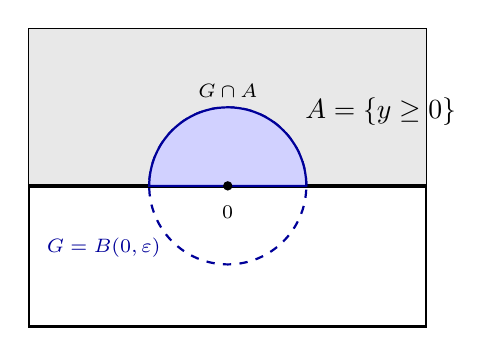
\begin{tikzpicture}[scale=1.05]
\draw[thick] (-2.4,-1.7) rectangle (2.4,1.9);
\node at (-2.1,1.6) {$\R^2$};
\fill[gray!18] (-2.4,0) rectangle (2.4,1.9);
\draw[very thick] (-2.4,0)--(2.4,0);
\node at (1.85,0.9) {$A=\{y\ge0\}$};
% bola centrada en el origen
\draw[blue!60!black,thick,dashed] (0,0) circle (0.95);
\fill[blue!18,draw=blue!60!black,thick] (0.95,0) arc (0:180:0.95) -- cycle;
\node[pt] at (0,0) {};
\node[below] at (0,-0.12) {\scriptsize $0$};
\node[blue!60!black] at (-1.5,-0.75) {\scriptsize $G=B(0,\varepsilon)$};
\node at (0,1.15) {\scriptsize $G\cap A$};
\end{tikzpicture}
\figtit{Figura 10. El semidisco $G\cap A$ \emph{es} abierto en el subespacio $A$ (es la traza de un abierto de $\R^2$), pero no es abierto en $\R^2$: los puntos del borde inferior no tienen ninguna bola de $\R^2$ contenida en él.}
\end{figure}

\begin{intuicion}
``Abierto'' no es una propiedad del conjunto solo: es una propiedad \emph{relativa al espacio en el que se lo mira}. $[0,1)$ no es abierto en $\R$, pero sí lo es en el subespacio $[0,2]$. Por eso siempre hay que decir ``abierto \emph{en}''. La Prop.~\ref{pr:subesp}(iii) da la única situación en la que se puede olvidar la distinción: cuando $A$ mismo es abierto en $X$.
\end{intuicion}

\begin{teorema}[Caracterizaciones equivalentes \fnt{EJ, Cap.\ 3, Prop.\ 3.1.2--3.1.3, pp.\,14--15 (impresas 17--18)}]
Sea $(X,\tp)$, $A\subseteq X$ e $i:A\to X$ la inclusión. Las tres descripciones siguientes definen la misma topología sobre $A$:
\begin{enumerate}[label=(\arabic*),leftmargin=2.2em,itemsep=0pt]
\item $\tp_A=\{U\cap A: U\in\tp\}$;
\item $\tp_A$ es la topología \emph{menos fina} sobre $A$ que hace continua la inclusión $i:A\to X$;
\item $\tp_A$ es la \emph{única} topología sobre $A$ que satisface la propiedad universal
\[
(\star)\quad \forall Z \text{ espacio topológico},\ \forall f:Z\to A:\qquad f \text{ es continua} \iff i\circ f:Z\to X \text{ es continua}.
\]
\end{enumerate}
\end{teorema}

\begin{proof}[Demostración de $(\star)$ y de la unicidad]
$(\star)$: si $f$ es continua, $i\circ f$ lo es por composición. Recíprocamente, si $i\circ f$ es continua y $V\in\tp_A$, escribimos $V=U\cap A=i^{-1}(U)$ con $U\in\tp$; entonces $f^{-1}(V)=f^{-1}(i^{-1}(U))=(i\circ f)^{-1}(U)$ es abierto, luego $f$ es continua.

Unicidad: sea $\tp^\ast$ otra topología en $A$ con $(\star)$. Aplicando $(\star)$ a $Z=(A,\tp^\ast)$ y $f=1_A$ (continua), se obtiene que $i:(A,\tp^\ast)\to X$ es continua. Ahora aplicando $(\star)$ para $\tp_A$ con $Z=(A,\tp^\ast)$ y $f=1_A$, la continuidad de $i:(A,\tp^\ast)\to X$ da que $1_A:(A,\tp^\ast)\to (A,\tp_A)$ es continua, es decir $\tp_A\subseteq\tp^\ast$. Intercambiando los roles se obtiene $\tp^\ast\subseteq\tp_A$.
\end{proof}

\begin{observacion}
El esquema de esta demostración (``una construcción caracterizada por una propiedad universal es única salvo isomorfismo, y se prueba aplicando la propiedad a la identidad en ambas direcciones'') es el mismo que reaparece en topología producto y cociente.
\end{observacion}

\begin{proposicion}[Propiedades básicas \fnt{GT 2.7.2--2.7.5, pp.\,32--33; EJ Obs.\ 3.1.4, p.\,14}]\label{pr:subesp}
Sea $A\subseteq X$ subespacio.
\begin{enumerate}[label=(\roman*),leftmargin=2.2em,itemsep=0pt]
\item Si $g:X\to Y$ es continua, $g|_A=g\circ i$ es continua.
\item Si $h:Z\to X$ es continua con $h(Z)\subseteq A$, la correstricción $h|^A:Z\to A$ es continua (consecuencia de $(\star)$).
\item Si $A$ es abierto en $X$, todo abierto de $(A,\tp_A)$ es abierto de $X$; ídem con cerrados. En general esto es falso: $A=\{(x,y):y\ge0\}\subseteq\R^2$ y $G\cap A$ con $G$ una bola centrada en el origen. \fnt{GT Ej.\ 2.7.3, p.\,32}
\item Si $B\subseteq A\subseteq X$: $\cl{B}^{A}=\cl{B}^{X}\cap A$.
\item Si $(X,d)$ es métrico, la topología de la métrica restringida coincide con la topología relativa, pues $B_{d|_A}(a,\varepsilon)=\Bola{a}{\varepsilon}\cap A$.
\end{enumerate}
\lgc{g:X\to Y\ \text{continua}\Rightarrow g|_A=g\circ i\ \text{continua};\qquad
h:Z\to X\ \text{continua}\wedge h(Z)\subseteq A\Rightarrow h|^{A}\ \text{continua};\\
A\in\tp\Rightarrow\big(V\in\tp_A\Rightarrow V\in\tp\big);\qquad
B\subseteq A:\ \cl B^{\,A}=\cl B^{\,X}\cap A;\qquad B_{d|_A}(a,\varepsilon)=\Bola{a}{\varepsilon}\cap A.}
\end{proposicion}

\begin{proposicion}[Intervalos: no hay abiertos-cerrados propios \fnt{GT 2.7.6, p.\,33} \noentra{va con conexidad (\S\ref{sec:bolzano}); todavía no dictado}]
Si $J\subseteq\R$ es un intervalo de cualquier tipo (incluida la recta), los únicos subconjuntos de $(J,\text{eucl.})$ simultáneamente abiertos y cerrados son $\emptyset$ y $J$. (Es la conexión de los intervalos, anticipada.)
\lgc{J\subseteq\R\ \text{intervalo}\ \wedge\ C\subseteq J\ \text{abierto y cerrado en } J\ \Rightarrow\ C=\emptyset\ \vee\ C=J.}
\end{proposicion}

\begin{teorema}[Bolzano topológico \fnt{GT 2.8.3, p.\,35} \noentra{va con conexidad (\S\ref{sec:bolzano}); todavía no dictado}]
Para $(X,\tp)$ son equivalentes:
\begin{enumerate}[label=(\alph*),leftmargin=2.2em,itemsep=0pt]
\item los únicos abiertos-cerrados de $X$ son $\emptyset$ y $X$;
\item si $f:X\to\R$ es continua y $a,b\in f(X)$ con $a\le b$, entonces $[a,b]\subseteq f(X)$;
\item si $f:X\to\R$ es continua y toma un valor negativo y otro positivo, entonces se anula.
\end{enumerate}
Combinado con la proposición anterior, se recupera el teorema de Bolzano clásico para intervalos.
\lgc{\big[\forall C\subseteq X\ (C\ \text{abierto y cerrado}\Rightarrow C\in\{\emptyset,X\})\big]\\
\iff \big[\forall f:X\to\R\ \text{continua}:\ a,b\in f(X)\ \wedge\ a\le b\ \Rightarrow\ [a,b]\subseteq f(X)\big]\\
\iff \big[\forall f:X\to\R\ \text{continua}:\ \exists x_1,x_2\ f(x_1)<0<f(x_2)\ \Rightarrow\ \exists x_0\ f(x_0)=0\big].}
\end{teorema}

\begin{observacion}[Cómo se usa]
La implicación (c)$\Rightarrow$(a) se prueba con $\chi$-tipo: si existiera $A\ne\emptyset,X$ abierto y cerrado, la función que vale $+1$ en $A$ y $-1$ fuera es continua (sus preimágenes son $\emptyset,A,X-A,X$) y no se anula. Es el mismo cálculo que en el ejercicio sobre $\chi_A$ (guía de continuidad, A.1).
\end{observacion}

%======================================================================
\section{Topología producto}\label{sec:prod}

\noindent Tema de la clase 9 (10/9/2026). No entró en el primer parcial: se evalúa en el segundo, junto con conexidad o compacidad. \textbf{GT} sólo trabaja productos de $\R^n$ con las distancias suma, euclídea y del máximo (\S\ref{sec:unif} y Prop.~\ref{pr:coord}); acá se hace el producto de dos espacios topológicos \emph{cualesquiera}, siguiendo el apunte \textbf{TP} de la cátedra y \textbf{MS} \S5.4. Todo lo que se dice para dos factores vale igual para una cantidad finita de factores.

\begin{proposicion}[Continuidad chequeada en una base del codominio \fnt{TP p.\,4; clase 9, Prop.\ 2.1}]\label{pr:contbase}
Sea $f:(X,\tp_X)\to(Y,\tp_Y)$ una función y sea $\beta$ una base de $\tp_Y$ fijada. Si la preimagen de cada elemento de $\beta$ es abierta en $X$, entonces $f$ es continua. (Es la caracterización (4) del Teorema~\ref{th:contab}; la recíproca es inmediata porque $\beta\subseteq\tp_Y$.)
\lgc{\beta\ \text{base de }\tp_Y\ \wedge\ \forall B\in\beta:\ f^{-1}(B)\in\tp_X\ \Longrightarrow\ \forall G\in\tp_Y:\ f^{-1}(G)\in\tp_X.}
\end{proposicion}

\begin{proof}
Sea $G\in\tp_Y$ y sea $x\in f^{-1}(G)$, es decir $f(x)\in G$. Como $\beta$ es base, existe $B\in\beta$ con $f(x)\in B\subseteq G$. Entonces $x\in f^{-1}(B)$ (definición de preimagen), $f^{-1}(B)\subseteq f^{-1}(G)$ (la preimagen respeta inclusiones) y $f^{-1}(B)$ es abierto (hipótesis). Luego $x\in\intr f^{-1}(G)$. Como $x$ era cualquiera, $f^{-1}(G)=\intr f^{-1}(G)$ es abierto.
\end{proof}

\begin{observacion}[Caso particular: bolas \fnt{TP p.\,4}]
Si $Y$ es métrico, alcanza con que $f^{-1}(\Bola{y}{r})$ sea abierto para toda bola. No hace falta que la preimagen de una bola sea una bola: basta que sea \emph{abierta}.
\end{observacion}

\subsection{La base de rectángulos y la topología producto}

\begin{definicion}[Rectángulos abiertos \fnt{TP p.\,1; MS \S5.4, p.\,66}]
Sean $(X,\tp_X)$ e $(Y,\tp_Y)$ espacios topológicos. Sobre el conjunto $X\times Y=\{(x,y):\ x\in X,\ y\in Y\}$ se considera la familia de los \emph{rectángulos abiertos} (``abierto por abierto'')
\[
\beta_{X\times Y}=\{U\times V:\ U\in\tp_X,\ V\in\tp_Y\}.
\]
\lgc{W\in\beta_{X\times Y}\iff \exists U\in\tp_X\ \exists V\in\tp_Y:\ W=U\times V.}
\end{definicion}

\begin{proposicion}[Los rectángulos son base \fnt{TP p.\,1; MS \S5.4, p.\,66; clase 9, Prop.\ 3.2}]\label{pr:rectbase}
$\beta_{X\times Y}$ cumple \textbf{(B1)} y \textbf{(B2)}; por lo tanto es base de una topología sobre $X\times Y$.
\lgc{\textbf{(B1)}\ \ \forall (x,y)\in X\times Y:\ (x,y)\in X\times Y\in\beta_{X\times Y};\\
\textbf{(B2)}\ \ (U_1\times V_1)\cap(U_2\times V_2)=(U_1\cap U_2)\times(V_1\cap V_2)\in\beta_{X\times Y}.}
\end{proposicion}

\begin{proof}
(B1): el propio $X\times Y$ es un rectángulo abierto, porque $X\in\tp_X$ e $Y\in\tp_Y$ (el todo es abierto en cualquier topología). (B2): si $(x,y)\in(U_1\times V_1)\cap(U_2\times V_2)$, se propone $B_3=(U_1\cap U_2)\times(V_1\cap V_2)$. Es básico porque $U_1\cap U_2\in\tp_X$ y $V_1\cap V_2\in\tp_Y$ (intersección finita de abiertos); contiene a $(x,y)$ porque $x\in U_1\cap U_2$ e $y\in V_1\cap V_2$; y está contenido en $B_1\cap B_2$ (de hecho es igual).
\end{proof}

\begin{definicion}[Topología producto \fnt{TP pp.\,1--2; MS \S5.4, p.\,66, ``de Tychonov''}]
La \emph{topología producto} $\tp_{X\times Y}$ (también $\tp_{prod}$; en \textbf{MS}, $\tp_X\times\tp_Y$ o $\tp_{Tyc}$) es la generada por la base $\beta_{X\times Y}$. Por el criterio de base (\S\ref{sec:bases}) tiene dos lecturas: $G$ es abierto si es \emph{unión} de rectángulos abiertos, o si \emph{cada punto} de $G$ tiene un rectángulo abierto alrededor metido en $G$.
\lgc{G\in\tp_{X\times Y}\iff G=\bigcup_{\alpha\in\Lambda}U_\alpha\times V_\alpha\ \ \text{con } U_\alpha\in\tp_X,\ V_\alpha\in\tp_Y\\
\iff \forall (x,y)\in G\ \ \exists U\in\tp_X\ \exists V\in\tp_Y:\ (x,y)\in U\times V\subseteq G.}
Salvo aviso, todo producto de este apunte lleva la topología producto.
\end{definicion}

\begin{observacion}[El error frecuente \fnt{TP p.\,2; clase 9, Obs.\ 3.4 y 4.2}]\label{ob:errorprod}
Es \emph{falso} que todo abierto de $X\times Y$ sea de la forma $U\times V$: en $\R^2$ un disco es abierto y no es un rectángulo. Tampoco vale $G=\pi_X(G)\times\pi_Y(G)$ (ver la definición de proyección abajo): el producto de las ``sombras'' de $G$ sobre los ejes es un rectángulo en general mucho más grande que $G$. Lo único que se puede asegurar es lo de la definición. Por eso el método de trabajo de toda la sección es: \emph{lo que haya que probar sobre un abierto cualquiera del producto, se prueba sobre los rectángulos y se arrastra por uniones} (o se usa la Prop.~\ref{pr:contbase}).
\end{observacion}

\begin{figure}[ht]
\centering
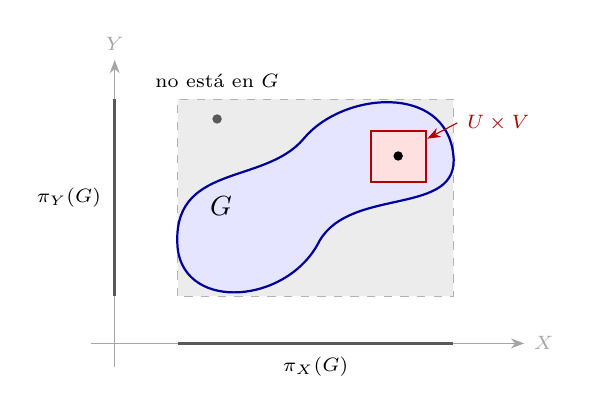
\begin{tikzpicture}[scale=1.0]
\draw[ejes] (-0.3,0)--(5.2,0) node[right]{\scriptsize $X$};
\draw[ejes] (0,-0.3)--(0,3.6) node[above]{\scriptsize $Y$};
% sombras
\fill[gray!15] (0.8,0.6) rectangle (4.3,3.1);
\draw[gray!60,dashed] (0.8,0.6) rectangle (4.3,3.1);
\draw[very thick,gray!70!black] (0.8,0)--(4.3,0);
\draw[very thick,gray!70!black] (0,0.6)--(0,3.1);
\node[below] at (2.55,-0.05) {\scriptsize $\pi_X(G)$};
\node[left] at (-0.05,1.85) {\scriptsize $\pi_Y(G)$};
% blob G
\draw[abierto] (0.8,1.2) .. controls (0.9,0.4) and (2.2,0.5) .. (2.6,1.3)
  .. controls (3.0,2.0) and (4.4,1.6) .. (4.3,2.4)
  .. controls (4.2,3.3) and (2.9,3.2) .. (2.4,2.6)
  .. controls (1.9,2.0) and (0.7,2.3) .. (0.8,1.2);
\node at (1.35,1.75) {$G$};
% rectangulo basico
\draw[red!70!black,thick,fill=red!12] (3.25,2.05) rectangle (3.95,2.7);
\node[pt] at (3.6,2.38) {};
\node[red!70!black,right] at (4.35,2.8) {\scriptsize $U\times V$};
\draw[->,>=Stealth,thin,red!70!black] (4.35,2.8)--(3.97,2.6);
% punto fuera
\node[pt,fill=gray!70!black] at (1.3,2.85) {};
\node[above] at (1.3,3.12) {\scriptsize no está en $G$};
\end{tikzpicture}
\figtit{Figura 11. Un abierto $G$ de $X\times Y$ no es un rectángulo, ni es el producto $\pi_X(G)\times\pi_Y(G)$ de sus sombras (el rectángulo gris, que agrega puntos que no están en $G$). Lo único seguro: cada punto de $G$ tiene un rectángulo básico $U\times V$ alrededor, dentro de $G$.}
\end{figure}

\begin{observacion}[Finitos factores, $\R^n$, y por qué no infinitos \fnt{TP p.\,2; MS Ejemplos 5.3, p.\,66; clase 9, Obs.\ 3.5--3.6} \noentra{se enuncia, no se demuestra}]\label{ob:prodfin}
\begin{lista}
\item La misma construcción da la topología producto de $X_1\times\dots\times X_n$, con base los $U_1\times\dots\times U_n$; y $(X\times Y)\times Z$ y $X\times(Y\times Z)$ resultan la misma.
\item La topología usual de $\R^n$ es la producto de $n$ copias de $(\R,\tp_u)$. Más en general, si $(X,d)$ e $(Y,\rho)$ son métricos, las distancias del máximo, de la suma y euclídea sobre $X\times Y$ inducen \emph{la topología producto} (compárese con la Prop.\ de métricas sobre el producto en \S\ref{sec:unif}).
\item $\tp_{dis}\times\tp_{dis}=\tp_{dis}$ (los $\{x\}\times\{y\}$ son abiertos) e $\tp_{ind}\times\tp_{ind}=\tp_{ind}$ (los únicos rectángulos son $\emptyset$ y $X\times Y$).
\item En (B2) se usó que $U_1\cap U_2$ es abierto. Con infinitos factores habría que intersecar infinitos abiertos, y ahí se rompe: el producto infinito es otra teoría, fuera del curso.
\end{lista}
\end{observacion}

\subsection{Proyecciones}

\begin{definicion}[Proyecciones \fnt{TP p.\,1; MS Prop.\ 5.9, p.\,66}]
Las \emph{proyecciones} de $X\times Y$ son $\pi_X:X\times Y\to X$, $\pi_X(x,y)=x$, y $\pi_Y:X\times Y\to Y$, $\pi_Y(x,y)=y$. (En \textbf{TP}: $\Pi_X,\Pi_Y$; en \textbf{MS}: $p_X,p_Y$; en \textbf{GT}, para $\R^n$: $p_i$.)
\lgc{\pi_X(x,y)=x;\qquad \pi_Y(x,y)=y.}
\end{definicion}

\begin{proposicion}[Tubos \fnt{TP pp.\,1--2; clase 9, Teo.\ 4.3}]\label{pr:tubos}
Para $U\subseteq X$ y $V\subseteq Y$, la preimagen de $U$ por $\pi_X$ es el tubo vertical $U\times Y$, la de $V$ por $\pi_Y$ es el tubo horizontal $X\times V$, y todo rectángulo es la intersección de sus dos tubos. Además, proyectar un rectángulo con lados no vacíos devuelve el lado.
\lgc{\pi_X^{-1}(U)=U\times Y;\qquad \pi_Y^{-1}(V)=X\times V;\qquad U\times V=\pi_X^{-1}(U)\cap\pi_Y^{-1}(V);\\
V\ne\emptyset\Rightarrow \pi_X(U\times V)=U;\qquad U\ne\emptyset\Rightarrow \pi_Y(U\times V)=V.}
\end{proposicion}

\begin{proof}
$\pi_X^{-1}(U)=\{(x,y): \pi_X(x,y)\in U\}=\{(x,y): x\in U\}=U\times Y$, e igual con $\pi_Y$. Luego $(U\times Y)\cap(X\times V)=(U\cap X)\times(Y\cap V)=U\times V$. Si $V\ne\emptyset$, para cada $x\in U$ se elige $y\in V$ y resulta $x=\pi_X(x,y)$.
\end{proof}

\begin{figure}[ht]
\centering
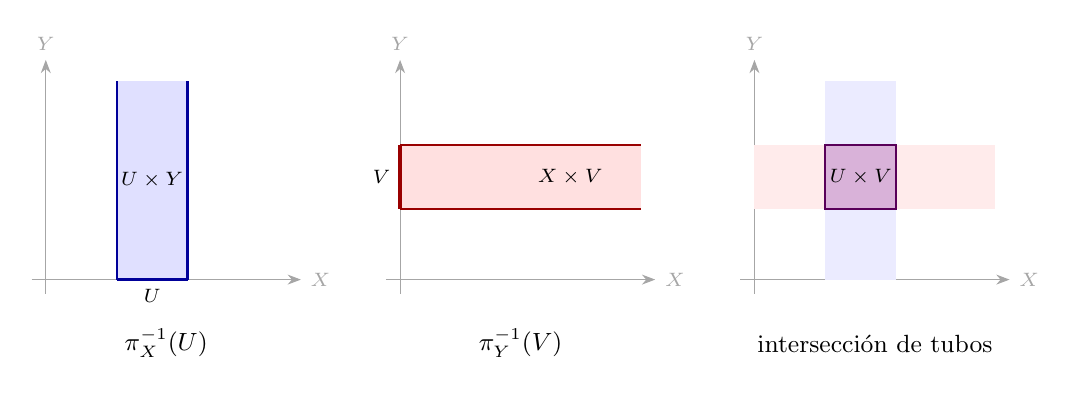
\begin{tikzpicture}[scale=0.9]
\begin{scope}
\draw[ejes] (-0.2,0)--(3.6,0) node[right]{\scriptsize $X$};
\draw[ejes] (0,-0.2)--(0,3.1) node[above]{\scriptsize $Y$};
\fill[blue!12] (1.0,0) rectangle (2.0,2.8);
\draw[blue!60!black,thick] (1.0,0)--(1.0,2.8) (2.0,0)--(2.0,2.8);
\draw[very thick,blue!60!black] (1.0,0)--(2.0,0);
\node[below] at (1.5,0) {\scriptsize $U$};
\node at (1.5,1.4) {\scriptsize $U\times Y$};
\node at (1.7,-0.9) {\small $\pi_X^{-1}(U)$};
\end{scope}
\begin{scope}[xshift=5cm]
\draw[ejes] (-0.2,0)--(3.6,0) node[right]{\scriptsize $X$};
\draw[ejes] (0,-0.2)--(0,3.1) node[above]{\scriptsize $Y$};
\fill[red!12] (0,1.0) rectangle (3.4,1.9);
\draw[red!60!black,thick] (0,1.0)--(3.4,1.0) (0,1.9)--(3.4,1.9);
\draw[very thick,red!60!black] (0,1.0)--(0,1.9);
\node[left] at (0,1.45) {\scriptsize $V$};
\node at (2.4,1.45) {\scriptsize $X\times V$};
\node at (1.7,-0.9) {\small $\pi_Y^{-1}(V)$};
\end{scope}
\begin{scope}[xshift=10cm]
\draw[ejes] (-0.2,0)--(3.6,0) node[right]{\scriptsize $X$};
\draw[ejes] (0,-0.2)--(0,3.1) node[above]{\scriptsize $Y$};
\fill[blue!8] (1.0,0) rectangle (2.0,2.8);
\fill[red!8] (0,1.0) rectangle (3.4,1.9);
\fill[violet!30] (1.0,1.0) rectangle (2.0,1.9);
\draw[violet!70!black,thick] (1.0,1.0) rectangle (2.0,1.9);
\node at (1.5,1.45) {\scriptsize $U\times V$};
\node at (1.7,-0.9) {\small intersección de tubos};
\end{scope}
\end{tikzpicture}
\figtit{Figura 12. Los tubos del pizarrón. La preimagen por una proyección es un tubo; un rectángulo es la intersección de dos tubos. Esta cuenta es la que mueve todas las demostraciones de la sección.}
\end{figure}

\begin{teorema}[La menos fina con proyecciones continuas \fnt{TP p.\,2; clase 9, Teo.\ 4.3; GT 2.8.11, p.\,38}]\label{th:menosfina}
\begin{enumerate}[label=(\roman*),leftmargin=2.2em,itemsep=0pt]
\item $\pi_X:(X\times Y,\tp_{X\times Y})\to(X,\tp_X)$ y $\pi_Y:(X\times Y,\tp_{X\times Y})\to(Y,\tp_Y)$ son continuas;
\item si $\sigma$ es otra topología en $X\times Y$ que hace continuas a $\pi_X$ y $\pi_Y$, entonces $\tp_{X\times Y}\subseteq\sigma$.
\end{enumerate}
\lgc{\pi_X,\pi_Y\ \text{continuas en } \tp_{X\times Y};\qquad
\big(\pi_X,\pi_Y\ \text{continuas en } \sigma\big)\ \Rightarrow\ \tp_{X\times Y}\subseteq\sigma;\\
\tp_{X\times Y}=\min\big\{\sigma\ \text{topología en } X\times Y:\ \pi_X,\pi_Y\ \text{continuas}\big\}.}
\end{teorema}

\begin{proof}
(i) Si $U\in\tp_X$, $\pi_X^{-1}(U)=U\times Y$ es un rectángulo abierto (Prop.~\ref{pr:tubos}), luego abierto. Igual para $\pi_Y$.
(ii) Sea $G\in\tp_{X\times Y}$; se escribe $G=\bigcup_\alpha U_\alpha\times V_\alpha$ y, como $\sigma$ es cerrada por uniones, basta ver cada $U_\alpha\times V_\alpha\in\sigma$ (\emph{truco: bajar el problema a la base}). Pero $U_\alpha\times V_\alpha=\pi_X^{-1}(U_\alpha)\cap\pi_Y^{-1}(V_\alpha)$ es intersección de dos abiertos de $\sigma$, por ser las proyecciones continuas en $\sigma$.
\end{proof}

\begin{observacion}[Subbase de tubos, y la analogía con el subespacio \fnt{TP p.\,1; clase 9, Obs.\ 4.4}]
Los tubos $\{\pi_X^{-1}(U)\}\cup\{\pi_Y^{-1}(V)\}$ forman una \emph{subbase} de $\tp_{X\times Y}$ cuyas intersecciones finitas son los rectángulos. Es el mismo esquema que la topología de subespacio (\S\ref{sec:sub}): allí, la menos fina que hace continua a la \emph{inclusión} $i:A\to X$; acá, la menos fina que hace continuas a las \emph{proyecciones}. La discreta sobre $X\times Y$ también las hace continuas, pero ``no conserva información'' de $X$ e $Y$.
\end{observacion}

\begin{teorema}[Continuidad hacia un producto \fnt{TP p.\,3; MS Prop.\ 5.10, p.\,66; GT 2.8.12, p.\,39}]\label{th:contprod}
Sea $Z$ un espacio topológico y $f:Z\to X\times Y$. Entonces $f$ es continua si y sólo si sus dos coordenadas $\pi_X\circ f:Z\to X$ y $\pi_Y\circ f:Z\to Y$ son continuas.
\lgc{f:Z\to X\times Y\ \text{continua}\iff \pi_X\circ f\ \text{continua}\ \wedge\ \pi_Y\circ f\ \text{continua}.}
\end{teorema}

\begin{proof}
($\Rightarrow$) Composición de continuas: $f$ lo es por hipótesis y $\pi_X,\pi_Y$ por el Teo.~\ref{th:menosfina}(i).
($\Leftarrow$) Por la Prop.~\ref{pr:contbase} basta ver que la preimagen de cada rectángulo $U\times V$ ($U\in\tp_X$, $V\in\tp_Y$) es abierta en $Z$:
\[
f^{-1}(U\times V)=f^{-1}\big(\pi_X^{-1}(U)\cap\pi_Y^{-1}(V)\big)=f^{-1}\big(\pi_X^{-1}(U)\big)\cap f^{-1}\big(\pi_Y^{-1}(V)\big)=(\pi_X\circ f)^{-1}(U)\cap(\pi_Y\circ f)^{-1}(V),
\]
usando los tubos, que la preimagen respeta intersecciones, y que $f^{-1}(\pi_X^{-1}(U))=(\pi_X\circ f)^{-1}(U)$ (ambos son $\{z: \pi_X(f(z))\in U\}$). Los dos últimos conjuntos son abiertos por hipótesis, y su intersección también.
\end{proof}

\begin{figure}[ht]
\centering
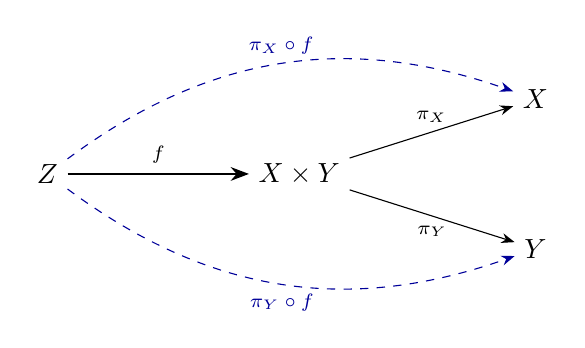
\begin{tikzpicture}[scale=1.0]
\node (Z) at (0,0) {$Z$};
\node (P) at (3.2,0) {$X\times Y$};
\node (X) at (6.2,0.95) {$X$};
\node (Y) at (6.2,-0.95) {$Y$};
\draw[->,>=Stealth,thick] (Z)--(P) node[midway,above]{\scriptsize $f$};
\draw[->,>=Stealth] (P)--(X) node[midway,above]{\scriptsize $\pi_X$};
\draw[->,>=Stealth] (P)--(Y) node[midway,below]{\scriptsize $\pi_Y$};
\draw[->,>=Stealth,dashed,blue!60!black] (Z) to[bend left=28] node[midway,above]{\scriptsize $\pi_X\circ f$} (X);
\draw[->,>=Stealth,dashed,blue!60!black] (Z) to[bend right=28] node[midway,below]{\scriptsize $\pi_Y\circ f$} (Y);
\end{tikzpicture}
\figtit{Figura 13. Una función hacia un producto es continua exactamente cuando sus dos coordenadas lo son. Es la propiedad universal del subespacio (\S\ref{sec:sub}) ``para el otro lado'': allá la flecha auxiliar era la inclusión, que entra a $X$; acá son las proyecciones, que salen del producto.}
\end{figure}

\begin{intuicion}
Para ver que algo cae adentro de un rectángulo alcanza con mirar por separado las dos coordenadas: $(a,b)\in U\times V$ sii $a\in U$ y $b\in V$. La continuidad hacia un producto es esa misma frase dicha para entornos: estar cerca de $(x,y)$ en el producto es estar cerca de $x$ \emph{y} cerca de $y$. Por eso la Prop.~\ref{pr:coord} de \textbf{GT} (continuidad hacia $\R^n$ coordenada a coordenada) es un caso particular.
\end{intuicion}

\begin{corolario}[Funciones armadas coordenada a coordenada \fnt{TP p.\,4, ejercicio 3}]\label{co:fxg}
Sean $f:X\to Z$, $g:Y\to W$ y $h:X\to Y'$ funciones continuas. Entonces son continuas
\begin{lista}
\item $(f,h):X\to Z\times Y'$, $(f,h)(x)=\big(f(x),h(x)\big)$;
\item $f\times g:X\times Y\to Z\times W$, $(f\times g)(x,y)=\big(f(x),g(y)\big)$;
\item las ``inclusiones a la altura $y_0$'' $x\mapsto(x,y_0)$ de $X$ en $X\times Y$, y las $y\mapsto(x_0,y)$ de $Y$ en $X\times Y$.
\end{lista}
\lgc{f,h\ \text{continuas}\Rightarrow (f,h)\ \text{continua};\qquad f,g\ \text{continuas}\Rightarrow f\times g\ \text{continua};\\
x\mapsto(x,y_0)\ \text{y}\ y\mapsto(x_0,y)\ \text{continuas}.}
\end{corolario}

\begin{proof}
Por el Teo.~\ref{th:contprod}, basta mirar coordenadas: las de $(f,h)$ son $f$ y $h$; las de $f\times g$ son $f\circ\pi_X$ y $g\circ\pi_Y$ (composiciones de continuas); las de $x\mapsto(x,y_0)$ son la identidad de $X$ y la constante $y_0$.
\end{proof}

\begin{proposicion}[Las proyecciones son abiertas \fnt{TP p.\,3; MS Prop.\ 5.9, p.\,66; versión general de GT Ej.\ 2.8.16, p.\,40}]\label{pr:proyab}
$\pi_X$ y $\pi_Y$ son aplicaciones abiertas: la imagen de un abierto del producto es abierta en el factor.
\lgc{\forall G\in\tp_{X\times Y}:\ \pi_X(G)\in\tp_X\ \wedge\ \pi_Y(G)\in\tp_Y.}
\end{proposicion}

\begin{proof}
Sea $G=\bigcup_\alpha U_\alpha\times V_\alpha$. La imagen de una unión es la unión de las imágenes (vale para cualquier función), así que $\pi_X(G)=\bigcup_\alpha\pi_X(U_\alpha\times V_\alpha)$. Cada $\pi_X(U_\alpha\times V_\alpha)$ es $U_\alpha$ si $V_\alpha\ne\emptyset$, y $\emptyset$ si no (Prop.~\ref{pr:tubos}): en ambos casos, abierto. Una unión de abiertos es abierta.
\end{proof}

\begin{contraejemplo}[Las proyecciones no son cerradas \fnt{GT Ej.\ 2.8.16(1), p.\,40; TP p.\,4; MS Obs.\ 5.4, p.\,66}]
En $\R^2=\R\times\R$ (usual $=$ producto), la rama de hipérbola $F=\{(x,y): y=\tfrac1x,\ x>0\}$ es cerrada, pero $\pi_X(F)=(0,+\infty)$ no es cerrado en $\R$: el $0$ es adherente y no está. ``No cerrada'' no quiere decir que nunca dé cerrado (un rectángulo cerrado se proyecta en un cerrado), sino que \emph{no siempre}. En \textbf{MS} el mismo ejemplo con la hipérbola completa: $\pi_X(\{xy=1\})=\R-\{0\}$.
\end{contraejemplo}

\begin{observacion}[Dos formas de ver que $F$ es cerrado]
Por complemento (\textbf{GT}: $\R^2-F$ es abierto) o por clausura (clase: $\cl F=F$, porque la curva se acerca al eje $y$ pero nunca llega a $x=0$); son la misma afirmación por la dualidad de \S\ref{sec:top}. En un métrico, la forma más cómoda de escribirlo es con sucesiones (Teo.~\ref{th:clsuc}): si $(x_n,1/x_n)\to(a,b)$, entonces $x_n\to a$ y $1/x_n\to b$; como $x_n\cdot\tfrac1{x_n}=1$, pasando al límite $ab=1$, luego $a\ne0$, y $a\ge0$ por ser límite de positivos: $a>0$ y $b=1/a$. El límite está en $F$.
\end{observacion}

\subsection{Propiedades del producto (guía de productos)}

\noindent La docente pidió tenerlas demostradas o al menos conocidas (``guárdenselas'', clase 9): se usan en conexidad y compacidad.

\begin{proposicion}[Clausura e interior de un producto \fnt{TP p.\,4, ejercicio 1; MS Prop.\ 5.11, p.\,66}]\label{pr:clprod}
Sean $A\subseteq X$ y $B\subseteq Y$. Entonces la clausura del producto es el producto de las clausuras, y el interior del producto es el producto de los interiores.
\lgc{\cl{A\times B}=\cl A\times\cl B;\qquad \intr(A\times B)=\intr A\times\intr B.}
\end{proposicion}

\begin{proof}
\emph{Clausura}, $\subseteq$: $\cl A\times\cl B=\pi_X^{-1}(\cl A)\cap\pi_Y^{-1}(\cl B)$ es cerrado (preimágenes de cerrados por continuas) y contiene a $A\times B$; como $\cl{A\times B}$ es el menor cerrado que lo contiene, está incluido. $\supseteq$: sea $(x,y)$ con $x\in\cl A$, $y\in\cl B$. Alcanza con ver que todo rectángulo básico $U\times V\ni(x,y)$ corta a $A\times B$ (todo abierto que contiene al punto contiene un básico que lo contiene). Como $x\in\cl A$ y $U\ni x$ es abierto, hay $a\in U\cap A$; igual hay $b\in V\cap B$; y $(a,b)\in(U\times V)\cap(A\times B)$.

\emph{Interior}, $\supseteq$: $\intr A\times\intr B$ es un rectángulo abierto contenido en $A\times B$. $\subseteq$: si $(x,y)\in\intr(A\times B)$, hay un básico con $(x,y)\in U\times V\subseteq A\times B$; como $V\ni y$ no es vacío, $U\subseteq A$, luego $x\in\intr A$; igual $y\in\intr B$.
\end{proof}

\begin{corolario}
El producto de dos cerrados es cerrado, y el producto de dos abiertos es abierto. $A\times B$ es denso en $X\times Y$ si $A$ y $B$ son densos (por ejemplo, $\Q\times\Q$ en $\R^2$).
\end{corolario}

\begin{proposicion}[Hausdorff por Hausdorff es Hausdorff \fnt{TP p.\,4, ejercicio 2; MS Prop.\ 5.12, p.\,67}]\label{pr:t2prod}
Si $X$ e $Y$ son $T_2$, entonces $X\times Y$ es $T_2$. (\textbf{MS}: lo mismo vale para $T_1$, y también la recíproca, si los factores son no vacíos.)
\lgc{X,Y\ \text{son } T_2\ \Rightarrow\ X\times Y\ \text{es } T_2.}
\end{proposicion}

\begin{proof}
Sean $(x_1,y_1)\ne(x_2,y_2)$; entonces difieren en alguna coordenada, digamos $x_1\ne x_2$. Por $T_2$ en $X$ hay $U_1\ni x_1$, $U_2\ni x_2$ abiertos disjuntos. Los tubos $U_1\times Y$ y $U_2\times Y$ son abiertos, contienen a cada punto respectivamente y son disjuntos, porque $(U_1\times Y)\cap(U_2\times Y)=(U_1\cap U_2)\times Y=\emptyset$. Si difieren en la segunda coordenada, se usan tubos horizontales.
\end{proof}

%======================================================================
\section{Conexidad}\label{sec:conex}

\noindent Tema de la clase 10 (24/9/2026), la primera de la segunda mitad. Sigue \textbf{GT} cap.~4, \S\S4.4--4.5 (conexión topológica), salteando por ahora la conexión por caminos (\S\S4.1--4.3), los intervalos de $\R$ y Bolzano (\S\ref{sec:bolzano}) y las componentes conexas (\S4.6). El producto de conexos se hace con la topología producto de \S\ref{sec:prod}, no con la versión métrica de \textbf{GT}.

\begin{definicion}[Disconexo, conexo, subconjunto conexo \fnt{GT 4.4.1, p.\,78; MS Defs.\ 7.1--7.2, p.\,87}]
$(X,\tp)$ es \emph{disconexo} (en clase: \emph{no conexo}) si existen dos abiertos $U$ y $V$ no vacíos, disjuntos, que entre los dos cubren $X$; el par $(U,V)$ es una \emph{desconexión} de $X$ (en \textbf{MS}: separación no trivial). $X$ es \emph{conexo} si no es disconexo. Un subconjunto $A\subseteq X$ es \emph{conexo} si el subespacio $(A,\tp_A)$ es conexo: se lo mira como espacio en sí mismo, olvidando lo que hay afuera.
\lgc{X\ \text{disconexo}\iff \exists U,V\in\tp:\ U\ne\emptyset\ \wedge\ V\ne\emptyset\ \wedge\ U\cap V=\emptyset\ \wedge\ U\cup V=X;\\
X\ \text{conexo}\iff \neg\big(X\ \text{disconexo}\big);\qquad A\subseteq X\ \text{conexo}\iff (A,\tp_A)\ \text{conexo}.}
\end{definicion}

\begin{intuicion}
Conexo quiere decir ``de una sola pieza''. Pero la definición es \emph{negativa}: lo que se define es romperse en dos. Por eso probar que algo \emph{no} es conexo es fácil (se exhibe la desconexión), y probar que \emph{sí} lo es requiere herramientas: ``lo busqué un rato y no lo encontré'' no es argumento. Casi todas las demostraciones de esta sección son por el contrarrecíproco: se supone una desconexión y se fabrica otra donde no puede haberla.
\end{intuicion}

\begin{ejemplo}[Ejemplos de referencia \fnt{GT Ej.\ 4.4.3 y Prop.\ 4.5.4, pp.\,78 y 81; MS Ejemplos 7.1, p.\,88; clase 10, Ejs.\ 2.2 y 3.2}]\label{ej:conex}
\begin{lista}
\item $\emptyset$ y los unitarios son conexos en cualquier espacio: no admiten dos abiertos no vacíos y disjuntos.
\item Un espacio discreto con más de un punto es disconexo: $(\{x\},\ X-\{x\})$ es una desconexión. Más aún, en un discreto los únicos subconjuntos conexos no vacíos son los unitarios.
\item En la indiscreta todo subconjunto es conexo.
\item Si dos abiertos no vacíos de $X$ siempre se cortan, $X$ es conexo: la cofinita sobre un $X$ infinito, la conumerable sobre $\R$, las de punto incluido y punto añadido.
\item $\R-\{0\}$ (subespacio de $\R$) es disconexo: $(-\infty,0)$ y $(0,+\infty)$ son abiertos en él y lo desconectan. En $(\R,\tp_u)$ los conexos son exactamente los intervalos (\S\ref{sec:bolzano}).
\end{lista}
\end{ejemplo}

\begin{proposicion}[Desconectar un subconjunto con abiertos del espacio grande \fnt{clase 10, Obs.\ 2.3; forma de trabajo de la cátedra, no figura en GT}]\label{pr:GH}
Sea $A\subseteq(X,\tp)$. Entonces $A$ es no conexo si y sólo si existen $G,H$ abiertos \emph{de $X$} tales que: los dos cortan a $A$, no se cortan \emph{dentro de $A$}, y entre los dos cubren a $A$.
\lgc{A\ \text{no conexo}\iff \exists G,H\in\tp:\ \underbrace{G\cap A\ne\emptyset\ \wedge\ H\cap A\ne\emptyset}_{\text{(1)}}\ \wedge\ \underbrace{G\cap H\cap A=\emptyset}_{\text{(2)}}\ \wedge\ \underbrace{A\subseteq G\cup H}_{\text{(3)}}.}
\end{proposicion}

\begin{proof}
Por definición, $A$ es no conexo sii hay $U,V\in\tp_A$ no vacíos, disjuntos, con $U\cup V=A$; y los abiertos de $A$ son $U=G\cap A$, $V=H\cap A$ con $G,H\in\tp$. Se traduce cada condición: $U\ne\emptyset\iff G\cap A\ne\emptyset$ (ídem $V$); $U\cap V=(G\cap A)\cap(H\cap A)=G\cap H\cap A$; y $U\cup V=(G\cup H)\cap A$, que es igual a $A$ sii $A\subseteq G\cup H$.
\end{proof}

\begin{observacion}
$G$ y $H$ \emph{pueden cortarse} entre sí, siempre que no lo hagan sobre $A$; y pueden salirse de $A$. Así, dos cuadrados separados en $\R^2$ se desconectan con dos discos que se superponen en el medio, fuera de los cuadrados (Figura 14). Esta proposición es la herramienta de todas las demostraciones de la sección: una vez que se tienen $G$ y $H$ uno se olvida del subespacio.
\end{observacion}

\begin{figure}[ht]
\centering
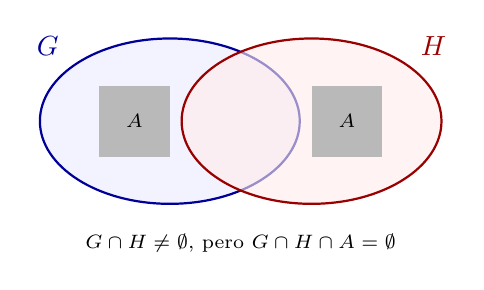
\begin{tikzpicture}[scale=1.0]
\draw[blue!60!black,thick,fill=blue!8,fill opacity=0.6] (-0.9,0) ellipse (1.65 and 1.05);
\draw[red!60!black,thick,fill=red!8,fill opacity=0.6] (0.9,0) ellipse (1.65 and 1.05);
\fill[gray!55] (-1.8,-0.45) rectangle (-0.9,0.45);
\fill[gray!55] (0.9,-0.45) rectangle (1.8,0.45);
\node at (-1.35,0) {\scriptsize $A$};
\node at (1.35,0) {\scriptsize $A$};
\node[blue!60!black] at (-2.45,0.95) {$G$};
\node[red!60!black] at (2.45,0.95) {$H$};
\node[align=center] at (0,-1.55) {\scriptsize $G\cap H\ne\emptyset$, pero $G\cap H\cap A=\emptyset$};
\end{tikzpicture}
\figtit{Figura 14. La desconexión con abiertos del espacio grande: $G$ y $H$ se superponen en el medio, pero no sobre $A$; cada uno se lleva un cuadrado y entre los dos cubren $A$.}
\end{figure}

\begin{proposicion}[Conexo $\iff$ no hay abiertos-cerrados propios \fnt{GT 4.4.2, p.\,78; MS Lema 7.1, p.\,87}]\label{pr:conexclopen}
$(X,\tp)$ es conexo si y sólo si los únicos subconjuntos simultáneamente abiertos y cerrados son $\emptyset$ y $X$. Equivalentemente (contrarrecíproco, como se dictó): $X$ es no conexo sii existe un abierto y cerrado que no es ni vacío ni todo. Por la Prop.~\ref{pr:clopen}, también: $X$ es conexo sii ningún subconjunto propio no vacío tiene frontera vacía.
\lgc{X\ \text{conexo}\iff \forall U\subseteq X\ \big(U\in\tp\ \wedge\ U\ \text{cerrado}\Rightarrow U=\emptyset\ \vee\ U=X\big);\\
X\ \text{no conexo}\iff \exists U\in\tp:\ U\ \text{cerrado}\ \wedge\ U\ne\emptyset\ \wedge\ U\ne X.}
\end{proposicion}

\begin{proof}
($\Rightarrow$ del contrarrecíproco) Si $(U,V)$ es una desconexión, $V=X-U$ (unión todo e intersección vacía). Entonces $U$ es abierto (hipótesis) y cerrado ($X-U=V$ es abierto), no vacío, y distinto de $X$ porque $X-U=V\ne\emptyset$.
($\Leftarrow$) Si $U$ es abierto y cerrado con $U\ne\emptyset,X$, sea $V=X-U$: es abierto porque $U$ es cerrado, $U\cup V=X$, $U\cap V=\emptyset$, $U\ne\emptyset$ y $V\ne\emptyset$ porque $U\ne X$. Luego $(U,V)$ desconecta a $X$.
\end{proof}

\begin{observacion}[Erratas de GT \fnt{clase 10, Obs.\ 3.3}]
La demostración impresa en \textbf{GT} p.\,78 escribe $X=(X-A)\cap A$ donde va $\cup$, y cierra la segunda parte con ``por tanto $(X,T)$ es conexo'' cuando lo que se probó es que existe un abierto-cerrado propio. El contenido es el de arriba.
\end{observacion}

\begin{proposicion}[Un conexo no puede partirse por un abierto-cerrado \fnt{MS Prop.\ 7.4, p.\,88}]\label{pr:conexlado}
Si $C\subseteq X$ es conexo y $A\subseteq X$ es abierto y cerrado, entonces $C$ queda entero de un lado: $C\subseteq A$ o $C\subseteq X-A$.
\lgc{C\ \text{conexo}\ \wedge\ A\in\tp\ \wedge\ A\ \text{cerrado}\ \Rightarrow\ C\subseteq A\ \vee\ C\subseteq X-A.}
\end{proposicion}

\begin{proof}
Si $C$ cortara a $A$ y a $X-A$, los abiertos $G=A$ y $H=X-A$ cumplirían (1), (2) y (3) de la Prop.~\ref{pr:GH} y desconectarían a $C$.
\end{proof}

\subsection{Imagen continua y funciones a un discreto}

\begin{proposicion}[La imagen continua de un conexo es conexa \fnt{GT 4.4.7, p.\,79; MS Teo.\ 7.5, p.\,88}]\label{pr:imconex}
Sea $f:(X,\tp)\to(Y,\tp')$ continua y $A\subseteq X$ conexo. Entonces $f(A)$ es conexo. En particular, si $X$ es conexo y $f$ es sobreyectiva, $Y$ es conexo; y la conexidad es una propiedad topológica (\textbf{MS} Cor.\ 7.6).
\lgc{f\ \text{continua}\ \wedge\ A\ \text{conexo}\ \Rightarrow\ f(A)\ \text{conexo};\qquad X\cong Y\Rightarrow\big(X\ \text{conexo}\iff Y\ \text{conexo}\big).}
\end{proposicion}

\begin{proof}
Por el contrarrecíproco: si $f(A)$ no es conexo, $A$ tampoco. Por la Prop.~\ref{pr:GH} en $Y$ hay $G,H\in\tp'$ con $G\cap f(A)\ne\emptyset$, $H\cap f(A)\ne\emptyset$, $G\cap H\cap f(A)=\emptyset$ y $f(A)\subseteq G\cup H$. Por continuidad $f^{-1}(G),f^{-1}(H)\in\tp$; se verifica que desconectan a $A$:
\begin{lista}
\item[(1)] si $y\in G\cap f(A)$, es $y=f(a)$ con $a\in A$, y $a\in f^{-1}(G)\cap A$. Igual con $H$.
\item[(2)] $f^{-1}(G)\cap f^{-1}(H)\cap A\subseteq f^{-1}(G)\cap f^{-1}(H)\cap f^{-1}(f(A))=f^{-1}\big(G\cap H\cap f(A)\big)=f^{-1}(\emptyset)=\emptyset$, usando $A\subseteq f^{-1}(f(A))$ y que la preimagen respeta intersecciones.
\item[(3)] $A\subseteq f^{-1}(f(A))\subseteq f^{-1}(G\cup H)=f^{-1}(G)\cup f^{-1}(H)$.
\end{lista}
\end{proof}

\begin{figure}[ht]
\centering
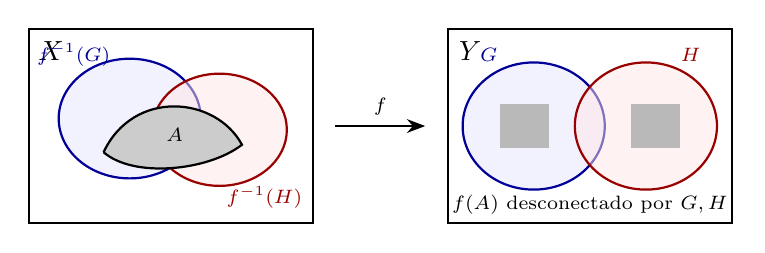
\begin{tikzpicture}[scale=0.95]
\begin{scope}
\draw[thick] (-1.9,-1.3) rectangle (1.9,1.3); \node at (-1.6,1.0) {$X$};
\draw[abierto,fill opacity=0.5] (-0.55,0.1) ellipse (0.95 and 0.8);
\draw[cerrado,fill opacity=0.5] (0.65,-0.05) ellipse (0.9 and 0.75);
\draw[thick,fill=gray!40] (-0.9,-0.35) .. controls (-0.5,0.5) and (0.6,0.4) .. (0.95,-0.25) .. controls (0.5,-0.6) and (-0.5,-0.7) .. (-0.9,-0.35);
\node at (0.05,-0.12) {\scriptsize $A$};
\node[blue!60!black] at (-1.3,0.95) {\scriptsize $f^{-1}(G)$};
\node[red!60!black] at (1.25,-0.95) {\scriptsize $f^{-1}(H)$};
\end{scope}
\draw[->,>=Stealth,thick] (2.2,0)--(3.4,0) node[midway,above]{\scriptsize $f$};
\begin{scope}[xshift=5.6cm]
\draw[thick] (-1.9,-1.3) rectangle (1.9,1.3); \node at (-1.6,1.0) {$Y$};
\draw[abierto,fill opacity=0.5] (-0.75,0) ellipse (0.95 and 0.85);
\draw[cerrado,fill opacity=0.5] (0.75,0) ellipse (0.95 and 0.85);
\fill[gray!55] (-1.2,-0.3) rectangle (-0.55,0.3);
\fill[gray!55] (0.55,-0.3) rectangle (1.2,0.3);
\node at (0,-1.05) {\scriptsize $f(A)$ desconectado por $G,H$};
\node[blue!60!black] at (-1.35,0.95) {\scriptsize $G$};
\node[red!60!black] at (1.35,0.95) {\scriptsize $H$};
\end{scope}
\end{tikzpicture}
\figtit{Figura 15. Si $G$ y $H$ desconectan a $f(A)$, sus preimágenes (abiertas por continuidad) desconectan a $A$. Las continuas tiran abiertos para atrás: una desconexión arriba produce una desconexión abajo.}
\end{figure}

\begin{corolario}[Topología menos fina \fnt{MS Lema 7.2, p.\,88}]
Si $(X,\tp_1)$ es conexo y $\tp_2\subseteq\tp_1$, entonces $(X,\tp_2)$ es conexo: es la imagen de $1_X:(X,\tp_1)\to(X,\tp_2)$, continua por la Prop.~\ref{pr:idcont}. (Con menos abiertos, cuesta más desconectar.)
\end{corolario}

\begin{definicion}[Espacio discreto \fnt{GT 4.5.2 y Ej.\ 4.5.3, p.\,81}]
$(X,\tp)$ es \emph{discreto} si todos los unitarios $\{x\}$ son abiertos; equivalentemente, $\tp=\mathcal P(X)$ y todo subconjunto es abierto y cerrado. Todo $(X,d_D)$ es discreto, pues $B_{d_D}(x,1)=\{x\}$.
\lgc{(X,\tp)\ \text{discreto}\iff \forall x\in X:\ \{x\}\in\tp\iff \tp=\mathcal P(X).}
\end{definicion}

\begin{proposicion}[Conexo $\iff$ toda continua a un discreto es constante \fnt{GT 4.5.5, p.\,81; MS Lema 7.1(v), p.\,87}]\label{pr:conexdisc}
Para $(X,\tp)$ son equivalentes: (a) $X$ es conexo; (b) toda función continua $f:X\to Y$ con $Y$ discreto es constante. Basta tomar $Y=\{0,1\}$ con la discreta.
\lgc{X\ \text{conexo}\iff \forall (Y,\tp')\ \text{discreto}\ \forall f:X\to Y\ \text{continua}:\ f\ \text{es constante}.}
\end{proposicion}

\begin{proof}
(a)$\Rightarrow$(b): $f(X)$ es conexo (Prop.~\ref{pr:imconex}) y está en un discreto, luego tiene un solo punto (Ej.~\ref{ej:conex}): si tuviera dos, $y\ne y'$, el par $(\{y\},f(X)-\{y\})$ lo desconectaría. O sea $f$ es constante.
(b)$\Rightarrow$(a), por el absurdo: si $(U,V)$ desconecta a $X$, sea $Y=\{y_0,y_1\}$ discreto y $f=y_0$ en $U$, $f=y_1$ en $V$ (bien definida porque $U,V$ son disjuntos y cubren $X$). Es continua: las preimágenes de los cuatro abiertos de $Y$ son $\emptyset$, $X$, $U$, $V$, todos abiertos (o: lema del pegado con $U,V$ abiertos). Y no es constante porque $U,V\ne\emptyset$. Contradicción.
\end{proof}

\begin{observacion}
Es la misma idea que la función característica: $\chi_A:X\to\R$ es continua sii $A$ es abierto y cerrado (guía de continuidad A.1), y en un conexo eso sólo pasa con $A=\emptyset$ o $A=X$.
\end{observacion}

\subsection{La herramienta principal: dos puntos en un conexo}

\begin{proposicion}[Conexo $\iff$ dos puntos cualesquiera caben en un conexo \fnt{GT 4.5.6, pp.\,81--82; MS Cor.\ 7.10(ii), p.\,89}]\label{pr:dospuntos}
Para $(X,\tp)$ son equivalentes: (a) $X$ es conexo; (b) para todos $a,b\in X$ existe un conexo $C\subseteq X$ con $a,b\in C$. Para un subconjunto: $B\subseteq X$ es conexo sii para todos $a,b\in B$ existe un conexo $C$ con $a,b\in C\subseteq B$ (es la misma proposición aplicada al espacio $(B,\tp_B)$).
\lgc{X\ \text{conexo}\iff \forall a,b\in X\ \exists C\subseteq X:\ C\ \text{conexo}\ \wedge\ a,b\in C;\\
B\ \text{conexo}\iff \forall a,b\in B\ \exists C:\ C\ \text{conexo}\ \wedge\ a,b\in C\subseteq B.}
\end{proposicion}

\begin{proof}
(a)$\Rightarrow$(b): $C=X$.
(b)$\Rightarrow$(a), por el contrarrecíproco: si $(U,V)$ desconecta a $X$, se eligen $a\in U$ y $b\in V$, uno en cada pata. Sea $C$ cualquiera con $a,b\in C$. Entonces $U\cap C\ni a$, $V\cap C\ni b$, $U\cap V\cap C=\emptyset$ y $C\subseteq U\cup V=X$: por la Prop.~\ref{pr:GH}, los mismos $U,V$ desconectan a $C$. Ningún conjunto que contenga a $a$ y $b$ es conexo.
\end{proof}

\begin{intuicion}
Para la docente es ``la proposición más útil de toda esta parte'': para probar que algo es conexo, en lugar de pelear contra todas las desconexiones posibles, alcanza con conectar dos puntos cualesquiera \emph{con un conexo que ya se conoce} (una recta, una copia de un factor, una imagen continua\dots). Es el reemplazo topológico de ``unir dos puntos con un camino''.
\end{intuicion}

\subsection{Unión, intersección y clausura de conexos}

\begin{proposicion}[Unión de dos conexos que se cortan \fnt{GT 4.5.7, p.\,82 (caso de dos); MS Teo.\ 7.9, p.\,89}]\label{pr:unionconex}
Si $A,B\subseteq X$ son conexos y $A\cap B\ne\emptyset$, entonces $A\cup B$ es conexo.
\lgc{A,B\ \text{conexos}\ \wedge\ A\cap B\ne\emptyset\ \Rightarrow\ A\cup B\ \text{conexo}.}
\end{proposicion}

\begin{proof}
Por la Prop.~\ref{pr:conexdisc}, basta ver que toda $f:A\cup B\to Y$ continua con $Y$ discreto es constante. La restricción $f|_A$ es continua y $A$ es conexo, luego $f\equiv y_1$ en $A$; igual $f\equiv y_2$ en $B$. Tomando $z\in A\cap B$: $y_1=f(z)=y_2$. Luego $f$ es constante en $A\cup B$.
\end{proof}

\begin{proposicion}[Uniones de familias \fnt{GT 4.5.7--4.5.9, pp.\,82--83; MS Teo.\ 7.9 y Cor.\ 7.10, p.\,89; CX 5--7}]\label{pr:familias}
Sea $\{C_\alpha\}_{\alpha\in\Lambda}$ una familia de conexos de $X$. Su unión es conexa en cualquiera de estos casos:
\begin{enumerate}[label=(\alph*),leftmargin=2.2em,itemsep=0pt]
\item hay uno fijo $C_{\alpha_0}$ que corta a todos (el ``osito'': todas las orejas tocan la cabeza);
\item se cortan dos a dos; en particular, si $\bigcap_\alpha C_\alpha\ne\emptyset$;
\item la familia es una sucesión $C_1,C_2,\dots$ en la que cada uno corta al siguiente (el ``gusano'').
\end{enumerate}
\lgc{\text{(a)}\ \exists\alpha_0\ \forall\alpha:\ C_\alpha\cap C_{\alpha_0}\ne\emptyset;\quad
\text{(b)}\ \forall\alpha,\beta:\ C_\alpha\cap C_\beta\ne\emptyset;\quad
\text{(c)}\ \forall n:\ C_n\cap C_{n+1}\ne\emptyset\\
\Longrightarrow\ \textstyle\bigcup C_\alpha\ \text{conexo}.}
\end{proposicion}

\begin{proof}[Idea (la indicada en clase)]
Siempre con la Prop.~\ref{pr:dospuntos} para subconjuntos: dados $x,y$ en la unión, hay que meterlos en un conexo contenido en la unión, armado con la Prop.~\ref{pr:unionconex}. (a): $x\in C_\alpha$, $y\in C_\beta$; $C_\alpha\cup C_{\alpha_0}$ es conexo, y ese bloque corta a $C_\beta$ (porque $C_\beta$ corta a $C_{\alpha_0}$), luego $C_\alpha\cup C_{\alpha_0}\cup C_\beta$ es conexo y contiene a $x,y$. (b): directamente $C_\alpha\cup C_\beta$. (c): $x\in C_i$, $y\in C_j$ con $i\le j$; por inducción $C_i\cup\dots\cup C_k$ es conexo para cada $k\ge i$ (se agrega $C_{k+1}$, que corta a $C_k$), y con $k=j$ se tiene el conexo buscado. En (c) hace falta el orden: de $x$ a $y$ se llega en una cantidad \emph{finita} de pasos.
\end{proof}

\begin{observacion}[La intersección de conexos no es conexa en general \fnt{clase 10, Obs.\ 7.3}]
En $\R^2$, la circunferencia $S^1$ y el eje $x$ son conexos, pero se cortan en $\{(-1,0),(1,0)\}$, que no es conexo (dos puntos en un métrico: es discreto). Lo mismo con dos arcos que se cruzan dos veces. No quiere decir que nunca sea conexa; quiere decir que no se puede afirmar.
\end{observacion}

\begin{proposicion}[Sándwich: lo que está entre un conexo y su clausura es conexo \fnt{GT 4.4.8, p.\,80; MS Teo.\ 7.11, p.\,89}]\label{pr:sandwich}
Si $A\subseteq X$ es conexo y $A\subseteq B\subseteq\cl A$, entonces $B$ es conexo. En particular, la clausura de un conexo es conexa.
\lgc{A\ \text{conexo}\ \wedge\ A\subseteq B\subseteq\cl A\ \Rightarrow\ B\ \text{conexo};\qquad A\ \text{conexo}\Rightarrow\cl A\ \text{conexo}.}
\end{proposicion}

\begin{proof}
Por el contrarrecíproco: si $G,H$ desconectan a $B$ (Prop.~\ref{pr:GH}), desconectan también a $A$. (3) y (2) se heredan porque $A\subseteq B$: $A\subseteq B\subseteq G\cup H$ y $G\cap H\cap A\subseteq G\cap H\cap B=\emptyset$. Lo único que hay que ganar es (1): como $G\cap B\ne\emptyset$, hay $x\in G\cap B$; como $x\in B\subseteq\cl A$ y $G$ es un abierto que contiene a $x$, por definición de clausura $G\cap A\ne\emptyset$. Igual $H\cap A\ne\emptyset$.
\end{proof}

\begin{observacion}[Frontera e interior de un conexo \fnt{clase 10, Obs.\ 7.6}]
Ninguno de los dos hereda la conexidad. La frontera de $[1,2]$ es $\{1,2\}$, no conexa. Para el interior (quedó de tarea en clase): en $\R^2$, dos discos cerrados tangentes $A=\Bolac{(-1,0)}{1}\cup\Bolac{(1,0)}{1}$ forman un conexo (se cortan en el origen), pero $\intr A=\Bola{(-1,0)}{1}\cup\Bola{(1,0)}{1}$ es disconexo: el origen no es interior. (En $\R$ no hay contraejemplo: el interior de un intervalo es un intervalo.) Las herencias (2) y (3) de la demostración anterior van en contra cuando el conjunto se \emph{achica}.
\end{observacion}

\begin{ejemplo}[Usos típicos \fnt{MS Ejemplo 7.1, p.\,89}]
$\R^n$ es conexo: es la unión de las rectas por el origen, cada una homeomorfa a $\R$ y todas cortándose en $0$ (Prop.~\ref{pr:familias}(b)). Una bola abierta de $\R^n$ es conexa (homeomorfa a $\R^n$), luego la bola cerrada y todo lo que está entre ambas también (sándwich). Estos ejemplos usan que $\R$ es conexo, que se prueba con los intervalos (\S\ref{sec:bolzano}).
\end{ejemplo}

\subsection{Más consecuencias (guía de conexidad)}

\noindent Resultados que la guía \textbf{CX} pide probar y que salen en pocas líneas de lo anterior. Las demostraciones completas están en los ejercicios resueltos.

\begin{proposicion}[Basta que uno toque la clausura del otro \fnt{CX 2}]\label{pr:clunion}
Si $A$ y $B$ son conexos y la clausura de $A$ corta a $B$, entonces $A\cup B$ es conexo.
\lgc{A,B\ \text{conexos}\ \wedge\ \cl A\cap B\ne\emptyset\ \Rightarrow\ A\cup B\ \text{conexo}.}
\end{proposicion}

\begin{proof}
$C=A\cup(\cl A\cap B)$ está entre $A$ y $\cl A$, luego es conexo (sándwich); $C$ corta a $B$, luego $C\cup B=A\cup B$ es conexo (Prop.~\ref{pr:unionconex}).
\end{proof}

\begin{observacion}
No alcanza con $\cl A\cap\cl B\ne\emptyset$: $(0,1)$ y $(1,2)$.
\end{observacion}

\begin{proposicion}[Un conexo denso conecta todo lo que lo contiene \fnt{CX 1}]
Si $A\subseteq B\subseteq X$ con $A$ conexo y denso en $X$, entonces $B$ es conexo (sándwich con $\cl A=X$).
\lgc{A\ \text{conexo}\ \wedge\ \cl A=X\ \wedge\ A\subseteq B\ \Rightarrow\ B\ \text{conexo}.}
\end{proposicion}

\begin{proposicion}[Para salir de $B$ hay que cruzar su frontera \fnt{CX 14}]\label{pr:cruzafr}
Si $A$ es conexo y tiene puntos dentro y fuera de $B$, entonces $A$ corta a la frontera de $B$.
\lgc{A\ \text{conexo}\ \wedge\ A\cap B\ne\emptyset\ \wedge\ A\cap(X-B)\ne\emptyset\ \Rightarrow\ A\cap\fr B\ne\emptyset.}
\end{proposicion}

\begin{proof}
Si $A\cap\fr B=\emptyset$, entonces $A\subseteq\intr B\cup\ext B$ (partición de $X$ en interior, frontera y exterior). Un punto de $A\cap B$ no está en $\ext B$, luego está en $\intr B$; un punto de $A-B$ no está en $\intr B$, luego está en $\ext B$. Así $G=\intr B$ y $H=\ext B$ desconectan a $A$ (Prop.~\ref{pr:GH}).
\end{proof}

\begin{proposicion}[El gráfico de una continua \fnt{CX 8}]
Si $X$ es conexo y $f:X\to Y$ es continua, su gráfico $\{(x,f(x)): x\in X\}$ es conexo en $X\times Y$: es la imagen de $x\mapsto(x,f(x))$, continua por tener coordenadas $1_X$ y $f$ (Teo.~\ref{th:contprod}).
\lgc{X\ \text{conexo}\ \wedge\ f\ \text{continua}\ \Rightarrow\ \{(x,f(x)):\ x\in X\}\ \text{conexo}.}
\end{proposicion}

\begin{definicion}[Totalmente disconexo \fnt{CX, p.\,2; MS Def.\ 7.3, p.\,88}]
$X$ es \emph{totalmente disconexo} si dos puntos distintos cualesquiera se pueden separar con una desconexión del espacio: abiertos disjuntos que cubren $X$, uno con cada punto. (\textbf{MS} lo define como ``sus únicos conexos son $\emptyset$ y los puntos''; con la definición de \textbf{CX}, esa es la Prop.\ siguiente.)
\lgc{X\ \text{totalmente disconexo}\iff \forall x\ne y\ \exists U,V\in\tp:\ x\in U\ \wedge\ y\in V\ \wedge\ U\cap V=\emptyset\ \wedge\ U\cup V=X.}
\end{definicion}

\begin{proposicion}[\fnt{CX 12 y 13}]
Si $X$ es totalmente disconexo, entonces es Hausdorff, y sus únicos conexos no vacíos son los unitarios.
\lgc{X\ \text{totalmente disconexo}\ \Rightarrow\ X\ \text{es } T_2\ \wedge\ \big(C\ne\emptyset\ \text{conexo}\Rightarrow |C|=1\big).}
\end{proposicion}

\begin{proof}
$T_2$ es parte de la definición. Si $C$ tuviera dos puntos, la desconexión $(U,V)$ que los separa también desconectaría a $C$ (Prop.~\ref{pr:GH}).
\end{proof}

\begin{ejemplo}[Totalmente disconexos no discretos \fnt{CX 11; MS Ejemplos 7.2, p.\,88}]
$\Q$ usual: entre $x<y$ hay un irracional $r$, y $(-\infty,r)\cap\Q$, $(r,\infty)\cap\Q$ los separan. Sorgenfrey: $(-\infty,y)$ y $[y,\infty)$ son abiertos. También el conjunto de Cantor.
\end{ejemplo}

\begin{ejemplo}[Peine del topólogo \fnt{\texttt{Peine-del-Topologo.pdf}} \noentra{usa que $[0,1]$ es conexo}]\label{ej:peine}
Sea $K=\{1/n: n\in\N\}$ y $E=(K\times[0,1])\cup([0,1]\times\{0\})$: dientes verticales sobre una base. $E$ es conexo (cada diente corta a la base, Prop.~\ref{pr:familias}(a)), y su clausura es el \emph{peine} $P=E\cup(\{0\}\times[0,1])$. Por el sándwich son conexos $P$ y el \emph{peine reducido} $R=E\cup\{(0,1)\}$. $R$ es el ejemplo estándar de conexo que \emph{no} es arcoconexo: ningún camino llega a $(0,1)$ (se verá con arcoconexidad, GT \S4.1; GT Ej.\ 4.2.8(4) da otro espacio con la misma propiedad).
\lgc{E\subseteq R\subseteq P=\cl E\ \wedge\ E\ \text{conexo}\ \Rightarrow\ R,P\ \text{conexos}.}
\end{ejemplo}

\begin{figure}[ht]
\centering
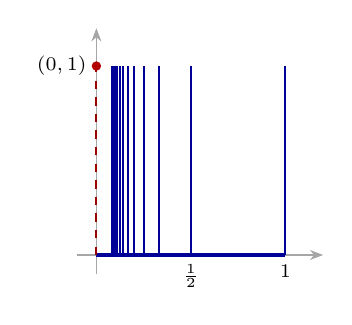
\begin{tikzpicture}[scale=2.4]
\draw[ejes] (-0.1,0)--(1.2,0); \draw[ejes] (0,-0.1)--(0,1.2);
\draw[very thick,blue!60!black] (0,0)--(1,0);
\foreach \n in {1,...,12}{\draw[blue!60!black,thick] ({1/\n},0)--({1/\n},1);}
\draw[red!60!black,thick,dashed] (0,0)--(0,1);
\node[pt,fill=red!70!black] at (0,1) {};
\node[left] at (0,1) {\scriptsize $(0,1)$};
\node[below] at (1,0) {\scriptsize $1$}; \node[below] at (0.5,0) {\scriptsize $\tfrac12$};
\end{tikzpicture}
\figtit{Figura 16. El peine: dientes en $x=1/n$ sobre la base $[0,1]\times\{0\}$ (azul). La clausura agrega el segmento $\{0\}\times[0,1]$ (rayado); el peine reducido agrega sólo el punto $(0,1)$. Todo lo que está entre $E$ y $\cl E$ es conexo.}
\end{figure}

\subsection{Producto de conexos}

\begin{proposicion}[Producto de conexos \fnt{clase 10, Prop.\ 8.1; MS Teo.\ 7.12, pp.\,89--90; reemplaza a GT 4.5.10, p.\,83}]\label{pr:prodconex}
Si $X$ e $Y$ son conexos, $X\times Y$ (con la topología producto) es conexo. Recíprocamente, si $X\times Y\ne\emptyset$ es conexo, $X$ e $Y$ lo son.
\lgc{X,Y\ \text{conexos}\ \Rightarrow\ X\times Y\ \text{conexo};\qquad X\times Y\ne\emptyset\ \text{conexo}\ \Rightarrow\ X,Y\ \text{conexos}.}
\end{proposicion}

\begin{proof}
Por la Prop.~\ref{pr:dospuntos}, dados $(x_1,y_1),(x_2,y_2)$ hay que meterlos en un conexo. La función $y\mapsto(x_2,y)$ de $Y$ en $X\times Y$ es continua (coordenadas: constante e identidad, Cor.~\ref{co:fxg}), así que su imagen $\{x_2\}\times Y$ es conexa (Prop.~\ref{pr:imconex}); igual $X\times\{y_1\}$, imagen de $x\mapsto(x,y_1)$. Las dos se cortan en $(x_2,y_1)$, luego la ``cruz'' $C=(X\times\{y_1\})\cup(\{x_2\}\times Y)$ es conexa (Prop.~\ref{pr:unionconex}), y contiene a $(x_1,y_1)$ y a $(x_2,y_2)$.
Recíproca: si $X\times Y\ne\emptyset$, $\pi_X$ es continua y sobreyectiva, así que $X=\pi_X(X\times Y)$ es conexo.
\end{proof}

\begin{figure}[ht]
\centering
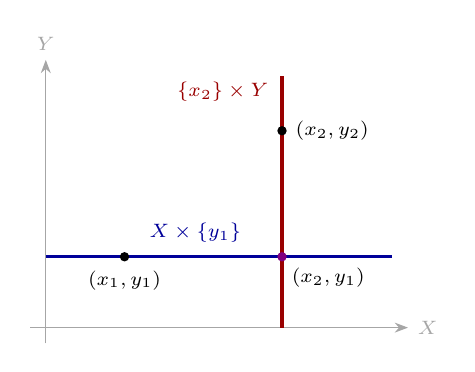
\begin{tikzpicture}[scale=1.0]
\draw[ejes] (-0.2,0)--(4.6,0) node[right]{\scriptsize $X$};
\draw[ejes] (0,-0.2)--(0,3.4) node[above]{\scriptsize $Y$};
\draw[blue!60!black,very thick] (0,0.9)--(4.4,0.9);
\draw[red!60!black,very thick] (3.0,0)--(3.0,3.2);
\node[pt] at (1.0,0.9) {}; \node[below] at (1.0,0.85) {\scriptsize $(x_1,y_1)$};
\node[pt] at (3.0,2.5) {}; \node[right] at (3.05,2.5) {\scriptsize $(x_2,y_2)$};
\node[pt,fill=violet] at (3.0,0.9) {}; \node[below right] at (3.0,0.88) {\scriptsize $(x_2,y_1)$};
\node[blue!60!black] at (1.9,1.2) {\scriptsize $X\times\{y_1\}$};
\node[red!60!black,left] at (2.95,3.0) {\scriptsize $\{x_2\}\times Y$};
\end{tikzpicture}
\figtit{Figura 17. La cruz del pizarrón: una copia de $X$ (horizontal) y una de $Y$ (vertical), conexas por ser imágenes continuas, que se cruzan en $(x_2,y_1)$. Hay que tomar una coordenada de cada punto para que las dos rayas se crucen.}
\end{figure}

\begin{observacion}
\textbf{GT} 4.5.10 prueba lo mismo sólo para métricos con $\delta^{\max}_2$, usando que $x_2\mapsto(x^0_1,x_2)$ es una isometría. La versión de clase no necesita métricas: sólo el Teorema~\ref{th:contprod}.
\end{observacion}

\begin{proposicion}[El producto menos un rectángulo propio \fnt{\texttt{Producto-de-Conexos.pdf}, p.\,2}]
Si $X,Y$ son conexos, $A\subsetneq X$ y $B\subsetneq Y$, entonces $(X\times Y)-(A\times B)$ es conexo.
\lgc{X,Y\ \text{conexos}\ \wedge\ A\ne X\ \wedge\ B\ne Y\ \Rightarrow\ (X\times Y)-(A\times B)\ \text{conexo}.}
\end{proposicion}

\begin{proof}
Con $a_0\notin A$ y $b_0\notin B$, la cruz $(\{a_0\}\times Y)\cup(X\times\{b_0\})$ queda dentro del conjunto y es conexa. Todo punto $(x,y)$ del conjunto tiene $x\notin A$ o $y\notin B$, así que su vertical $\{x\}\times Y$ o su horizontal $X\times\{y\}$ queda dentro y corta a la cruz. Se concluye con la Prop.~\ref{pr:familias}(a).
\end{proof}

\begin{observacion}[Arcoconexos \fnt{\texttt{Producto-de-Conexos.pdf}, p.\,2} \noentra{arcoconexidad todavía no dictada}]
El mismo apunte prueba que el producto de arcoconexos es arcoconexo: si $\alpha$ une $x_0$ con $x_1$ en $X$ y $\beta$ une $y_0$ con $y_1$ en $Y$, el camino $t\mapsto(\alpha(t),\beta(t))$ es continuo por el Cor.~\ref{co:fxg}.
\end{observacion}

%======================================================================
% Fragmento conexion2: se inserta al final de la sección de Conexidad,
% justo ANTES de \subsection{Lo que falta: intervalos de $\R$ y Bolzano}.
% Prefijo de labels: cc:
%======================================================================

\subsection{Conexión por caminos (arcoconexión)}\label{cc:caminos}

\noindent\noentra{todavía no dictado en clase} Sigue \textbf{GT} \S4.1 y \textbf{MS} \S7.3. En la guía \textbf{CX} se dice \emph{arcoconexo} para lo que \textbf{GT} llama \emph{conexo por caminos}; acá se usan las dos palabras como sinónimos (no se pide que el camino sea inyectivo). A diferencia de la conexión, es una propiedad \emph{positiva}: para probarla se exhibe algo (un camino), en lugar de descartar todas las desconexiones.

\begin{definicion}[Camino \fnt{GT 4.1.1, p.\,61; MS Def.\ 7.6, p.\,90} \noentra{todavía no dictado en clase}]\label{cc:defcamino}
Sea $(X,\tp)$ un espacio topológico y $x,y\in X$. Un \emph{camino de $x$ a $y$} en $X$ es una función continua $\alpha:[0,1]\to X$ (con $[0,1]$ con la topología usual) que empieza en $x$ y termina en $y$. Los puntos $x$ e $y$ son el \emph{origen} y el \emph{extremo} del camino.
\lgc{\alpha\ \text{camino de } x \text{ a } y \text{ en } X\iff \alpha:([0,1],\tp_u)\to(X,\tp)\ \text{continua}\ \wedge\ \alpha(0)=x\ \wedge\ \alpha(1)=y.}
\end{definicion}

\begin{definicion}[Conexo por caminos, arcoconexo \fnt{GT 4.1.2, p.\,61; MS Def.\ 7.7, p.\,91} \noentra{todavía no dictado en clase}]\label{cc:defarco}
$(X,\tp)$ es \emph{conexo por caminos} (o \emph{arcoconexo}) si para cualquier par de puntos $x,y\in X$ existe un camino en $X$ de $x$ a $y$. Un subconjunto $A\subseteq X$ es conexo por caminos si lo es el subespacio $(A,\tp_A)$, es decir, si dos puntos cualesquiera de $A$ se unen con un camino \emph{que no sale de $A$}.
\lgc{X\ \text{arcoconexo}\iff \forall x,y\in X\ \exists\alpha:[0,1]\to X\ \text{continua}:\ \alpha(0)=x\ \wedge\ \alpha(1)=y;\\
A\subseteq X\ \text{arcoconexo}\iff \forall x,y\in A\ \exists\alpha:[0,1]\to X\ \text{continua}:\ \alpha([0,1])\subseteq A\ \wedge\ \alpha(0)=x\ \wedge\ \alpha(1)=y.}
\end{definicion}

\begin{observacion}
En la versión para subconjuntos se usa que una $\alpha:[0,1]\to A$ es continua hacia $(A,\tp_A)$ si y sólo si es continua hacia $X$ (la topología de subespacio es la que hace continua a la inclusión y a las correstricciones, \S\ref{sec:sub}). Por eso se puede pensar el camino ``dentro de $X$'' y sólo pedir que su imagen quede en $A$.
\end{observacion}

\begin{ejemplo}[Intervalos y espacios normados \fnt{GT Ej.\ 4.1.3, p.\,61; MS Ejemplos 7.3(1), (4), p.\,91} \noentra{todavía no dictado en clase}]\label{cc:segmentos}
\begin{lista}
\item Todo intervalo $J\subseteq\R$ (de cualquier tipo, incluida la recta) es arcoconexo: si $x\le y$ están en $J$, entonces $[x,y]\subseteq J$, y el camino $\alpha(t)=(1-t)x+ty$ recorre $[x,y]$ de $x$ a $y$.
\item Todo espacio normado $(V,\norm{\cdot})$ con su distancia $d(u,v)=\norm{u-v}$ es arcoconexo: el \emph{segmento} $\alpha(t)=(1-t)x+ty$ es continuo, porque
$\norm{\alpha(t)-\alpha(s)}=\norm{(t-s)(y-x)}=|t-s|\,\norm{y-x}$, es decir, $\alpha$ es lipschitziana. En particular $(\R^n,d_2)$ es arcoconexo.
\item Más en general, todo subconjunto \emph{convexo} de un normado (bolas abiertas o cerradas, cubos, semiespacios\dots) es arcoconexo: el segmento entre dos de sus puntos no sale del conjunto.
\item Todo espacio indiscreto es arcoconexo: toda función hacia un indiscreto es continua, así que cualquier $\alpha$ con $\alpha(0)=x$ y $\alpha(1)=y$ sirve.
\end{lista}
\end{ejemplo}

\begin{observacion}[Errata menor de GT]
En \textbf{GT} 4.1.3(2) se propone $\delta\le\varepsilon/(\norm x+\norm y)$, que no está definido si $x=y=0$. La cuenta de arriba, con $\norm{y-x}$, evita el problema (y si $x=y$ el camino es constante).
\end{observacion}

\begin{proposicion}[Arcoconexo $\Rightarrow$ conexo \fnt{GT 4.1.4, p.\,62; MS Prop.\ 7.17, p.\,91} \noentra{todavía no dictado en clase}]\label{cc:arcoconexo}
Si $(X,\tp)$ es conexo por caminos, entonces es conexo; equivalentemente (Prop.~\ref{pr:conexclopen}), sus únicos abiertos-cerrados son $\emptyset$ y $X$. Lo mismo para subconjuntos: un $A\subseteq X$ arcoconexo es conexo.
\lgc{X\ \text{arcoconexo}\ \Rightarrow\ X\ \text{conexo};\qquad A\subseteq X\ \text{arcoconexo}\ \Rightarrow\ A\ \text{conexo}.}
\end{proposicion}

\begin{proof}
Por el absurdo: sea $(U,V)$ una desconexión de $X$, y $x\in U$, $y\in V$. Sea $\alpha$ un camino de $x$ a $y$. Por continuidad $\alpha^{-1}(U)$ y $\alpha^{-1}(V)$ son abiertos de $[0,1]$; son disjuntos y cubren $[0,1]$ (porque $U,V$ lo hacen con $X$), y no son vacíos: $0\in\alpha^{-1}(U)$, $1\in\alpha^{-1}(V)$. Entonces $[0,1]$ tendría un abierto-cerrado propio, lo que contradice la proposición de \textbf{GT} 2.7.6 (``Intervalos: no hay abiertos-cerrados propios'', \S\ref{sec:sub}).
Otra forma, con las herramientas de la sección: $\alpha([0,1])$ es conexo (imagen continua del conexo $[0,1]$, Prop.~\ref{pr:imconex}) y contiene a $x$ e $y$; se concluye con la Prop.~\ref{pr:dospuntos}.
\end{proof}

\begin{observacion}
La recíproca es falsa: el peine reducido del Ejemplo~\ref{ej:peine} es conexo y no es arcoconexo (se prueba en el Ejemplo~\ref{cc:peinered}); también la curva seno del topólogo $\{(x,\sin\frac1x):x>0\}\cup\big((-\infty,0]\times\{0\}\big)$ \fnt{MS Ej.\ 7.2, p.\,91} y el espacio de \textbf{GT} Ej.\ 4.2.8(4) (Ejemplo~\ref{cc:escalera}). En $\R$ las dos nociones coinciden: es la proposición ``Los conexos de la recta'' de \S\ref{sec:bolzano}, que en \textbf{GT} aparece primero en versión por caminos (\textbf{GT} 4.1.5, p.\,62) y después con conexión (\textbf{GT} 4.4.4).
\end{observacion}

\begin{proposicion}[La imagen continua de un arcoconexo es arcoconexa \fnt{GT 4.1.6, p.\,64; MS Teo.\ 7.19 y Cor.\ 7.20, pp.\,91--92} \noentra{todavía no dictado en clase}]\label{cc:imarco}
Sea $f:(X,\tp)\to(Y,\tp')$ continua y $A\subseteq X$ conexo por caminos. Entonces $f(A)$ es conexo por caminos. En particular, si $X$ es arcoconexo y $f$ es sobreyectiva, $Y$ es arcoconexo; y la arcoconexión es una propiedad topológica.
\lgc{f\ \text{continua}\ \wedge\ A\ \text{arcoconexo}\ \Rightarrow\ f(A)\ \text{arcoconexo};\qquad X\cong Y\Rightarrow\big(X\ \text{arcoconexo}\iff Y\ \text{arcoconexo}\big).}
\end{proposicion}

\begin{proof}
Dados $p,q\in f(A)$, se eligen $x,y\in A$ con $f(x)=p$, $f(y)=q$, y un camino $\alpha$ de $x$ a $y$ dentro de $A$. Entonces $f\circ\alpha:[0,1]\to Y$ es continua (composición de continuas), $(f\circ\alpha)(0)=p$, $(f\circ\alpha)(1)=q$, y su imagen $f(\alpha([0,1]))$ está en $f(A)$.
\end{proof}

\begin{definicion}[Camino inverso y yuxtaposición \fnt{GT 4.1.9, pp.\,65--66} \noentra{todavía no dictado en clase}]\label{cc:yuxta}
Sean $\alpha$ un camino de $x$ a $y$ y $\beta$ un camino de $y$ a $z$ en $X$ (el extremo de $\alpha$ es el origen de $\beta$). El \emph{camino inverso} de $\alpha$ es $\alpha^-$, que recorre $\alpha$ al revés; la \emph{yuxtaposición} (o concatenación) $\alpha*\beta$ recorre $\alpha$ a doble velocidad en la primera mitad del tiempo y $\beta$ en la segunda:
\lgc{\alpha^-(t)=\alpha(1-t);\qquad (\alpha*\beta)(t)=\begin{cases}\alpha(2t) & \text{si } 0\le t\le\frac12,\\ \beta(2t-1) & \text{si } \frac12\le t\le 1.\end{cases}}
\end{definicion}

\begin{proposicion}[``Estar unidos por un camino'' es de equivalencia \fnt{GT 4.1.9, pp.\,65--66; MS Def.\ 7.9, p.\,92} \noentra{todavía no dictado en clase}]\label{cc:equiv}
En $(X,\tp)$, la relación $x\sim y$ si existe un camino en $X$ de $x$ a $y$ es reflexiva, simétrica y transitiva. Más precisamente: los caminos constantes son caminos; si $\alpha$ es un camino de $x$ a $y$, $\alpha^-$ es un camino de $y$ a $x$; y si además $\beta$ es un camino de $y$ a $z$, $\alpha*\beta$ es un camino de $x$ a $z$.
\lgc{x\sim y\iff \exists\alpha:[0,1]\to X\ \text{continua}:\ \alpha(0)=x\ \wedge\ \alpha(1)=y;\\
x\sim x;\qquad x\sim y\Rightarrow y\sim x;\qquad x\sim y\ \wedge\ y\sim z\Rightarrow x\sim z.}
\end{proposicion}

\begin{proof}
Reflexiva: el camino constante $\alpha(t)=x$ es continuo. Simétrica: $\alpha^-=\alpha\circ\rho$ con $\rho(t)=1-t$ continua de $[0,1]$ en $[0,1]$, y $\alpha^-(0)=\alpha(1)=y$, $\alpha^-(1)=\alpha(0)=x$.
Transitiva: $\alpha*\beta$ está bien definida porque en $t=\frac12$ las dos fórmulas dan $\alpha(1)=y=\beta(0)$. Su restricción a $[0,\frac12]$ es $\alpha\circ(t\mapsto2t)$ y su restricción a $[\frac12,1]$ es $\beta\circ(t\mapsto2t-1)$, ambas continuas; como $[0,\frac12]$ y $[\frac12,1]$ son \emph{dos} cerrados que cubren $[0,1]$, el Lema del pegado (versión (b), con finitos cerrados; \S\ref{sec:unif}) da que $\alpha*\beta$ es continua. Además $(\alpha*\beta)(0)=\alpha(0)=x$ y $(\alpha*\beta)(1)=\beta(1)=z$.
\end{proof}

\begin{figure}[ht]
\centering
\begin{tikzpicture}[scale=1.0]
\draw[thick] (0,0)--(4,0); \node[pt] at (0,0){}; \node[pt] at (2,0){}; \node[pt] at (4,0){};
\node[below] at (0,0){\scriptsize $0$}; \node[below] at (2,0){\scriptsize $\frac12$}; \node[below] at (4,0){\scriptsize $1$};
\draw[blue!60!black,very thick] (0,0)--(2,0); \draw[red!60!black,very thick] (2,0)--(4,0);
\draw[->,>=Stealth] (4.4,0.2)--(5.6,0.6) node[midway,above]{\scriptsize $\alpha*\beta$};
\node[pt] (x) at (6.2,-0.3){}; \node[pt] (y) at (8.2,0.9){}; \node[pt] (z) at (10.2,0.0){};
\node[left] at (x){\scriptsize $x$}; \node[above] at (y){\scriptsize $y$}; \node[right] at (z){\scriptsize $z$};
\draw[blue!60!black,very thick] (6.2,-0.3) .. controls (6.8,0.9) and (7.4,-0.2) .. (8.2,0.9) node[pos=0.5,below right]{\scriptsize $\alpha$};
\draw[red!60!black,very thick] (8.2,0.9) .. controls (9.0,1.6) and (9.6,-0.9) .. (10.2,0.0) node[pos=0.55,below left]{\scriptsize $\beta$};
\end{tikzpicture}
\figtit{Figura 18. Yuxtaposición: en la primera mitad del tiempo se recorre $\alpha$ (azul) a doble velocidad, en la segunda $\beta$ (rojo). Pega bien porque las dos fórmulas coinciden en $t=\frac12$; la continuidad sale del lema del pegado con dos cerrados.}
\end{figure}

\begin{observacion}
Gracias a la transitividad, para probar que $X$ es arcoconexo alcanza con fijar un punto $x_0$ y unir \emph{cada} $x$ con $x_0$: si $\alpha_x$ va de $x_0$ a $x$, entonces $\alpha_x^-*\alpha_y$ va de $x$ a $y$. Es el análogo por caminos de la Prop.~\ref{pr:dospuntos}.
\end{observacion}

\begin{proposicion}[Uniones de arcoconexos \fnt{GT 4.1.10--4.1.12, pp.\,67--68} \noentra{todavía no dictado en clase}]\label{cc:uniones}
Sea $\{C_\alpha\}_{\alpha\in\Lambda}$ una familia de subconjuntos arcoconexos de $X$. Su unión es arcoconexa en cualquiera de estos casos (los mismos tres de la Prop.~\ref{pr:familias}, ahora con caminos):
\begin{enumerate}[label=(\alph*),leftmargin=2.2em,itemsep=0pt]
\item hay un $C_{\alpha_0}$ que corta a todos (\textbf{GT} 4.1.10);
\item se cortan dos a dos, en particular si $\bigcap_\alpha C_\alpha\ne\emptyset$ (\textbf{GT} 4.1.11);
\item es una sucesión $C_1,C_2,\dots$ en la que cada uno corta al siguiente (\textbf{GT} 4.1.12).
\end{enumerate}
En particular, la unión de dos arcoconexos que se cortan es arcoconexa.
\lgc{\text{(a)}\ \exists\alpha_0\ \forall\alpha:\ C_\alpha\cap C_{\alpha_0}\ne\emptyset;\quad
\text{(b)}\ \forall\alpha,\beta:\ C_\alpha\cap C_\beta\ne\emptyset;\quad
\text{(c)}\ \forall n:\ C_n\cap C_{n+1}\ne\emptyset\\
\Longrightarrow\ \textstyle\bigcup C_\alpha\ \text{arcoconexo}.}
\end{proposicion}

\begin{proof}
(a) Sean $x\in C_\alpha$ y $x'\in C_{\alpha'}$. Se eligen $x_0\in C_\alpha\cap C_{\alpha_0}$ y $x_0'\in C_{\alpha'}\cap C_{\alpha_0}$. Hay caminos de $x$ a $x_0$ dentro de $C_\alpha$, de $x_0$ a $x_0'$ dentro de $C_{\alpha_0}$ y de $x_0'$ a $x'$ dentro de $C_{\alpha'}$, todos dentro de la unión; su yuxtaposición (Prop.~\ref{cc:equiv}) une $x$ con $x'$ sin salir de la unión.
(b) Es (a) con $\alpha_0$ cualquiera.
(c) Por inducción $D_n=C_1\cup\dots\cup C_n$ es arcoconexo: $D_{n}=D_{n-1}\cup C_n$ y $D_{n-1}\cap C_n\supseteq C_{n-1}\cap C_n\ne\emptyset$ (caso de dos, que es (b)). Los $D_n$ son arcoconexos y todos contienen a $D_1=C_1\ne\emptyset$, así que por (b) su unión, que es $\bigcup_n C_n$, es arcoconexa.
\end{proof}

\begin{observacion}[Productos \fnt{GT Nota 4.1.8, p.\,65 y Prop.\ 4.1.7, p.\,64; MS Teo.\ 7.21, p.\,92} \noentra{todavía no dictado en clase}]
\textbf{GT} 4.1.7 prueba que el producto de dos (seudo)métricos arcoconexos es arcoconexo con $\delta^{\max}_2$, y la Nota 4.1.8 aclara que vale igual con $\delta_2^{\mathrm{taxi}}$, con $\delta_2^{\mathrm{eucl}}$, con la topología producto general y con finitos factores. La versión con topología producto ya está en este apunte: es la observación ``Arcoconexos'' al final de la subsección \emph{Producto de conexos} (camino $t\mapsto(\alpha(t),\beta(t))$, continuo por el Cor.~\ref{co:fxg}). La recíproca también vale, como para conexos (\textbf{MS} Teo.\ 7.21): si $X\times Y\ne\emptyset$ es arcoconexo, $X=\pi_X(X\times Y)$ e $Y=\pi_Y(X\times Y)$ lo son por la Prop.~\ref{cc:imarco}.
\end{observacion}

\begin{ejemplo}[Espacios arcoconexos conocidos \fnt{GT Ej.\ 4.1.13, pp.\,68--69; MS Ejemplos 7.3, p.\,91} \noentra{todavía no dictado en clase}]\label{cc:ejarco}
\begin{lista}
\item Un ``paralelepípedo'' $J_1\times\dots\times J_n\subseteq\R^n$ con los $J_i$ intervalos (en particular $\R^n$) es arcoconexo: producto de arcoconexos (observación anterior), o directamente porque es convexo.
\item El disco $\{(x,y): x^2+y^2\le1\}$ es arcoconexo: es convexo.
\item La circunferencia $S^1$ es arcoconexa: es la imagen del intervalo $[0,2\pi]$ por la continua $t\mapsto(\cos t,\sin t)$ (Prop.~\ref{cc:imarco}).
\item La esfera $S^2\subseteq\R^3$ es arcoconexa: cada hemisferio cerrado $E_\pm=S^2\cap\{\pm z\ge0\}$ es homeomorfo al disco por $(x,y,z)\mapsto(x,y)$, luego arcoconexo, y los dos se cortan en el ecuador (Prop.~\ref{cc:uniones}).
\item El cilindro $S^1\times\R$ es arcoconexo, por ser producto de arcoconexos.
\item \fnt{MS Ejemplos 7.3(3)} La arcoconexión \emph{no} es hereditaria: $\R$ es arcoconexo y $\R-\{0\}$ no lo es (ni siquiera es conexo, Ej.~\ref{ej:conex}).
\item \fnt{MS Ejemplos 7.3(4)} Si $A\subseteq\R^n$ es numerable y $n\ge2$, $\R^n-A$ es arcoconexo. Idea: dados $q\ne r$ fuera de $A$, para cada punto $s$ de la mediatriz de $[q,r]$ la poligonal $q\to s\to r$ es un camino; son no numerables y dos de ellas sólo comparten $q$ y $r$, así que el numerable $A$ no puede cortarlas a todas.
\end{lista}
\end{ejemplo}

\subsection{Componentes conexas por caminos y conexión local por caminos}\label{cc:compcam}

\noindent\noentra{todavía no dictado en clase} Sigue \textbf{GT} \S4.2 y \textbf{MS} \S7.4. \textbf{GT} escribe $C_x$ tanto para la componente conexa por caminos como para la componente conexa (\S4.6); acá, como en \textbf{MS}, se distinguen: $c(x)$ para la de caminos y $C(x)$ para la conexa.

\begin{definicion}[Componente conexa por caminos \fnt{GT 4.2.1, p.\,70; MS Def.\ 7.9, p.\,92} \noentra{todavía no dictado en clase}]\label{cc:defcompcam}
Sea $(X,\tp)$ y $x\in X$. La \emph{componente conexa por caminos} (o \emph{componente arcoconexa}) de $x$, $c(x)$, es el mayor subconjunto arcoconexo de $X$ que contiene a $x$: es arcoconexo, contiene a $x$, y contiene a todo arcoconexo que contenga a $x$.
\lgc{c(x)\ \text{arcoconexo}\ \wedge\ x\in c(x)\ \wedge\ \forall A\subseteq X\ \big(A\ \text{arcoconexo}\ \wedge\ x\in A\Rightarrow A\subseteq c(x)\big).}
\end{definicion}

\begin{proposicion}[Existe y es la clase de equivalencia de $x$ \fnt{GT Lema 4.2.2 y Prop.\ 4.2.3, p.\,70} \noentra{todavía no dictado en clase}]\label{cc:existecam}
Para todo $x\in X$ la componente $c(x)$ existe: es la unión de todos los arcoconexos que contienen a $x$. Y coincide con la clase de $x$ para la relación $\sim$ de la Prop.~\ref{cc:equiv}, es decir, con el conjunto de puntos que se pueden unir con $x$ por un camino en $X$.
\lgc{c(x)=\bigcup\{A\subseteq X:\ A\ \text{arcoconexo},\ x\in A\}=\{y\in X:\ \exists\ \text{camino en } X \text{ de } x \text{ a } y\}.}
\end{proposicion}

\begin{proof}
La familia de arcoconexos que contienen a $x$ no es vacía ($\{x\}$ está) y todos se cortan en $x$; por la Prop.~\ref{cc:uniones}(b) su unión $D$ es arcoconexa, contiene a $x$, y contiene a cada miembro de la familia: es el mayor, $D=c(x)$.
Sea $Z=\{y:\ x\sim y\}$. Si $y\in c(x)$, hay un camino de $x$ a $y$ dentro de $c(x)$, que es en particular un camino en $X$: $y\in Z$. Si $z\in Z$ y $\alpha$ es un camino en $X$ de $x$ a $z$, su imagen $\alpha([0,1])$ es arcoconexa (Prop.~\ref{cc:imarco}, porque $[0,1]$ lo es) y contiene a $x$ y $z$; luego $\alpha([0,1])\subseteq c(x)$ y $z\in c(x)$.
\end{proof}

\begin{observacion}
Atención con la segunda descripción: el camino de $x$ a $y$ se busca en todo $X$, pero entonces automáticamente se queda dentro de $c(x)$ (toda su imagen está en $c(x)$).
\end{observacion}

\begin{proposicion}[Propiedades de las componentes arcoconexas \fnt{GT 4.2.4, p.\,71; MS Def.\ 7.9, p.\,92} \noentra{todavía no dictado en clase}]\label{cc:propcam}
En $(X,\tp)$: $x\in c(x)$; $c(x)$ es arcoconexo; $c(x)$ es la clase de $x$ por $\sim$; y dos componentes arcoconexas o son iguales o son disjuntas. Es decir, las componentes arcoconexas forman una partición de $X$ (\textbf{MS} llama $\pi_0(X)$ al conjunto de esas clases).
\lgc{x\in c(x);\qquad c(x)\cap c(y)\ne\emptyset\ \Rightarrow\ c(x)=c(y);\qquad X=\bigcup_{x\in X}c(x).}
\end{proposicion}

\begin{proof}
Todo sale de que son las clases de equivalencia de $\sim$ (Prop.~\ref{cc:existecam}), y las clases de una relación de equivalencia forman una partición.
\end{proof}

\begin{proposicion}[Una imagen continua cae en una componente \fnt{GT 4.2.7, pp.\,71--72} \noentra{todavía no dictado en clase}]\label{cc:invcam}
Si $f:X\to Y$ es continua, $f(c(x))\subseteq c(f(x))$. Si $f$ es un homeomorfismo, $f(c(x))=c(f(x))$, y $f$ induce una biyección $c(x)\mapsto f(c(x))$ entre las componentes arcoconexas de $X$ y las de $Y$. En particular, el número de componentes arcoconexas es un invariante topológico.
\lgc{f\ \text{continua}\Rightarrow f(c(x))\subseteq c(f(x));\qquad f\ \text{homeomorfismo}\Rightarrow f(c(x))=c(f(x)).}
\end{proposicion}

\begin{proof}
$f(c(x))$ es arcoconexo (Prop.~\ref{cc:imarco}) y contiene a $f(x)$, luego está en $c(f(x))$. Si $f$ es homeomorfismo, lo mismo con $f^{-1}$ da $f^{-1}(c(f(x)))\subseteq c(x)$, o sea $c(f(x))\subseteq f(c(x))$. La correspondencia $c(x)\mapsto c(f(x))$ tiene inversa $c(y)\mapsto c(f^{-1}(y))$.
\end{proof}

\begin{definicion}[Localmente conexo por caminos \fnt{GT 4.2.5, p.\,71; MS Def.\ 7.8, p.\,91} \noentra{todavía no dictado en clase}]\label{cc:deflocarco}
$(X,\tp)$ es \emph{localmente conexo por caminos} (localmente arcoconexo) si todo entorno de cualquier punto contiene un entorno arcoconexo de ese punto; es decir, si cada punto tiene una base de entornos formada por arcoconexos (así lo define \textbf{MS}).
\lgc{X\ \text{loc.\ arcoconexo}\iff \forall x\in X\ \forall N\in\mathcal N_x\ \exists N'\in\mathcal N_x:\ N'\subseteq N\ \wedge\ N'\ \text{arcoconexo}.}
\end{definicion}

\begin{intuicion}
``Localmente'' no es ``un poco'': no alcanza con que cada punto tenga \emph{algún} entorno arcoconexo (el propio $X$ lo sería si es arcoconexo), sino que tiene que haberlos \emph{tan chicos como se quiera}. Por eso ser arcoconexo y ser localmente arcoconexo son independientes: $[-1,0)\cup(0,1]$ es localmente arcoconexo y no es arcoconexo; los espacios tipo peine son arcoconexos y no localmente arcoconexos.
\end{intuicion}

\begin{proposicion}[En un localmente arcoconexo las componentes arcoconexas son abiertas y cerradas \fnt{GT 4.2.6, p.\,71} \noentra{todavía no dictado en clase}]\label{cc:compabcam}
Si $(X,\tp)$ es localmente conexo por caminos, cada componente arcoconexa $c(x)$ es abierta y cerrada en $X$.
\lgc{X\ \text{loc.\ arcoconexo}\ \Rightarrow\ \forall x\in X:\ c(x)\in\tp\ \wedge\ c(x)\ \text{cerrado}.}
\end{proposicion}

\begin{proof}
Abierta: sea $y\in c(x)$; entonces $c(y)=c(x)$ (Prop.~\ref{cc:propcam}). Aplicando la definición al entorno $N=X$ de $y$ se obtiene un entorno $N'$ de $y$ arcoconexo; como contiene a $y$, $N'\subseteq c(y)=c(x)$. Así $c(x)$ es entorno de cada uno de sus puntos, o sea abierto.
Cerrada: su complemento es la unión de las demás componentes (son una partición), cada una abierta por lo anterior.
\end{proof}

\begin{observacion}
La demostración de \textbf{GT} para ``cerrada'' pasa por la clausura; la de arriba, por el complemento, es más corta y es la misma idea que se usa con las componentes conexas.
\end{observacion}

\begin{ejemplo}[Localmente arcoconexos \fnt{GT Ej.\ 4.2.8(1)--(2), p.\,72; CX 18} \noentra{todavía no dictado en clase}]\label{cc:ejlocarco}
\begin{lista}
\item $\R^n$ es arcoconexo y localmente arcoconexo: las bolas $\Bola{x}{r}$ son convexas, luego arcoconexas, y forman una base de entornos de $x$. Lo mismo vale para cualquier \emph{abierto} de $\R^n$ (las bolas chicas quedan adentro), y para cualquier normado.
\item $S^1$ y el disco cerrado son arcoconexos y localmente arcoconexos (alrededor de un punto de $S^1$, los arcos chicos son imágenes continuas de intervalos).
\item \fnt{CX 18} $[-1,0)\cup(0,1]\subseteq\R$ (la guía dice $(0,-1]$, errata por $(0,1]$) es localmente arcoconexo, y por lo tanto localmente conexo: cada punto tiene intervalos arbitrariamente chicos a su alrededor dentro del conjunto. No es conexo.
\item Un discreto es localmente arcoconexo: $\{x\}$ es un entorno arcoconexo de $x$ contenido en cualquier otro.
\end{lista}
\end{ejemplo}

\begin{ejemplo}[Arcoconexo pero no localmente arcoconexo \fnt{GT Ej.\ 4.2.8(3), pp.\,72--73 y Ej.\ 4.6.9(4), pp.\,86--87; CX 15} \noentra{todavía no dictado en clase}]\label{cc:peinecompleto}
Sea $X\subseteq\R^2$ la unión del eje $OX$, del eje $OY$ y de las rectas verticales $A_n=\{1/n\}\times\R$, $n\ge1$. Es arcoconexo: $OX$, $OY$ y los $A_n$ son rectas y todas cortan a $OX$ (Prop.~\ref{cc:uniones}(a)). No es localmente conexo (y menos aún localmente arcoconexo) en $p=(0,y_0)$ con $y_0\ne0$. En efecto, sea $0<r<|y_0|$, de modo que $\Bola{p}{r}$ no toca a $OX$, y sea $N\subseteq\Bola{p}{r}\cap X$ un entorno de $p$ en $X$. Contiene alguna $\Bola{p}{\delta}\cap X$, que contiene a $p_n=(1/n,y_0)$ para $n$ grande. Fijado un tal $n$, se toma $\lambda$ con $\frac1{n+1}<\lambda<\frac1n$: ningún punto de $X\cap\Bola{p}{r}$ tiene primera coordenada $\lambda$ (esos puntos están en $OY$ o en algún $A_k$). Entonces $G=\{(x,y): x<\lambda\}$ y $H=\{(x,y): x>\lambda\}$ son abiertos de $\R^2$ que cubren $N$, no se cortan, y $p\in G$, $p_n\in H$: desconectan a $N$ (Prop.~\ref{pr:GH}). Ningún entorno de $p$ dentro de $\Bola{p}{r}$ es conexo.
La guía pide lo mismo con el eje $Y$ y las rectas $y=nx$ \fnt{CX 15}: arcoconexo porque todas las rectas pasan por el origen, y no localmente arcoconexo en los puntos del eje $Y$ distintos del origen, con el mismo tipo de argumento.
\end{ejemplo}

\begin{ejemplo}[El peine reducido no es arcoconexo \fnt{\texttt{Peine-del-Topologo.pdf}; comparar GT Ej.\ 4.2.8(4)} \noentra{todavía no dictado en clase}]\label{cc:peinered}
Con la notación del Ejemplo~\ref{ej:peine}: $E=(K\times[0,1])\cup([0,1]\times\{0\})$ es arcoconexo (dientes y base son segmentos, y cada diente corta a la base: Prop.~\ref{cc:uniones}(a)); el peine $P=\cl E$ también (se agrega el segmento $\{0\}\times[0,1]$, que corta a la base). Pero el peine reducido $R=E\cup\{p\}$, $p=(0,1)$, que es conexo, \emph{no} es arcoconexo: sus componentes arcoconexas son $E$ y $\{p\}$.
\end{ejemplo}

\begin{proof}
Sea $\alpha:[0,1]\to R$ un camino con $\alpha(0)=p$; se ve que $\alpha$ es constante, así que ningún punto de $E$ se une con $p$. Sea $S=\alpha^{-1}(\{p\})$, que contiene a $0$.
$S$ es cerrado en $[0,1]$: $\{p\}$ es cerrado (en un métrico los puntos son cerrados) y $\alpha$ es continua.
$S$ es abierto en $[0,1]$: sea $t\in S$. Los puntos de $R$ en $W=\Bola{p}{\frac12}$ son $p$ y trozos de dientes $\{1/n\}\times(\frac12,1]$ (la base está a distancia $1$ de $p$). Por continuidad hay un intervalo $J\ni t$, abierto en $[0,1]$, con $\alpha(J)\subseteq W$. Si existiera $s\in J$ con $\alpha(s)\ne p$, sería $\alpha(s)=(1/n,y)$ para algún $n$. La primera coordenada $g=\pi_1\circ\alpha$ es continua en el intervalo de extremos $t$ y $s$ (contenido en $J$), con $g(t)=0$ y $g(s)=1/n$; por el teorema de Bolzano (del Análisis) toma el valor $\lambda=\frac{1}{n+1/2}\in(\frac1{n+1},\frac1n)$ en algún punto de $J$. Pero ningún punto de $R\cap W$ tiene primera coordenada $\lambda$. Absurdo: $\alpha(J)=\{p\}$ y $J\subseteq S$.
Como $[0,1]$ es conexo (\S\ref{sec:bolzano}) y $S$ es abierto, cerrado y no vacío, $S=[0,1]$: $\alpha$ es constante en $p$.
\end{proof}

\begin{observacion}[Moraleja: no hay ``sándwich'' para caminos \fnt{GT Nota 4.2.9, pp.\,75--76; CX 16}]\label{cc:nosandwich}
$E\subseteq R\subseteq\cl E$ con $E$ arcoconexo y $R$ no arcoconexo: la Prop.~\ref{pr:sandwich} no tiene versión por caminos. Además, la componente arcoconexa $\{p\}$ de $R$ es cerrada pero no abierta, y $E$ es abierta en $R$ pero no cerrada (su clausura en $R$ es $R$): a diferencia de las componentes conexas (Prop.~\ref{cc:propcomp}), las arcoconexas \emph{no tienen por qué ser cerradas}. La pregunta de \textbf{CX} 16 (``¿es arcoconexa la clausura de un arcoconexo?'') tiene respuesta negativa con el ejemplo siguiente de \textbf{GT} (con el peine la clausura $P$ sí resulta arcoconexa; lo que falla es el conjunto intermedio $R$).
\end{observacion}

\begin{ejemplo}[La escalera: conexo, no arcoconexo, y clausura de un arcoconexo \fnt{GT Ej.\ 4.2.8(4), pp.\,73--75, Ej.\ 4.4.5, p.\,79 y Nota 4.2.9, pp.\,75--76} \noentra{todavía no dictado en clase}]\label{cc:escalera}
En $\R^2$ sean $A_0=OY$ (el eje vertical), $A_n=\{1/n\}\times\R$ para $n\ge1$, y los peldaños horizontales $B_n=[\frac1{n+1},\frac1n]\times\{n\}$, que unen $A_{n+1}$ con $A_n$ a altura $n$. Sea $X=\bigcup_{n\ge0}A_n\cup\bigcup_{n\ge1}B_n$ y $H=X-A_0$. Entonces:
\begin{lista}
\item $H$ es arcoconexo: la sucesión $A_1,B_1,A_2,B_2,A_3,\dots$ es de arcoconexos y cada uno corta al siguiente (Prop.~\ref{cc:uniones}(c)).
\item $X$ es conexo: $H\subseteq X\subseteq\cl H$, porque cada $(0,y)\in A_0$ es límite de $(1/n,y)\in A_n$; se aplica el sándwich (Prop.~\ref{pr:sandwich}).
\item $X$ no es arcoconexo: no hay camino de un punto de $H$ a uno de $A_0$ (demostración abajo). Sus componentes arcoconexas son $H$ y $A_0$; $\cl H=X$, así que la clausura de un arcoconexo no tiene por qué ser arcoconexa (\textbf{CX} 16), y la componente $H$ no es cerrada.
\end{lista}
\end{ejemplo}

\begin{proof}[Demostración de que no es arcoconexo]
Supongamos que $\alpha:[0,1]\to X$ es continua con $\alpha(0)=q\in H$ y $\alpha(1)\in A_0$. La segunda coordenada $\pi_2\circ\alpha:[0,1]\to\R$ es continua, luego acotada (teorema de Weierstrass del Análisis): $|\pi_2(\alpha(t))|\le M$ para todo $t$. La primera coordenada de $q$ es positiva; se elige $n_0>M$ con $\frac1{n_0}<\pi_1(q)$ y $\lambda\in(\frac1{n_0+1},\frac1{n_0})$. Por Bolzano (del Análisis) aplicado a $\pi_1\circ\alpha$, que vale $\pi_1(q)>\lambda$ en $0$ y $0<\lambda$ en $1$, hay $t$ con $\pi_1(\alpha(t))=\lambda$. Pero los puntos de $X$ con primera coordenada $\lambda$ están sólo en el peldaño $B_{n_0}$, a altura $n_0>M$: absurdo.
\end{proof}

\begin{observacion}[Erratas de GT en 4.2.8(4)]
En la demostración impresa, $V$ debe ser $\{(x,y): x>\lambda\}$ (dice $y>\lambda$), y para que $p\in V$ hay que elegir $n_0$ también en función de $p$, como arriba. \textbf{GT} prueba la conexión de $X$ viendo que no hay abiertos-cerrados propios; el sándwich lo hace en una línea.
\end{observacion}

\begin{figure}[ht]
\centering
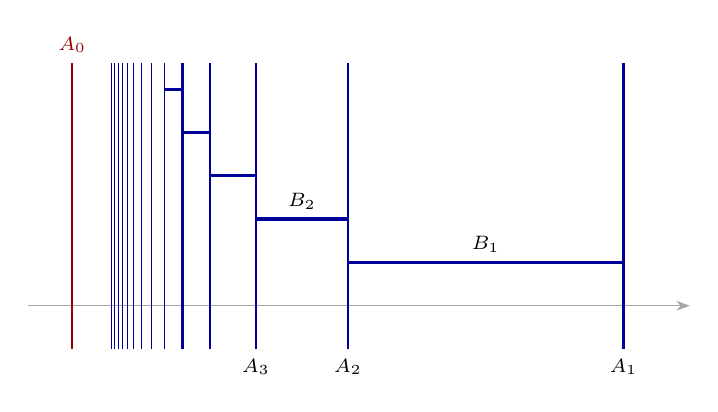
\begin{tikzpicture}[xscale=7,yscale=0.55]
\draw[ejes] (-0.08,0)--(1.12,0);
\draw[red!60!black,thick] (0,-1)--(0,5.6) node[above]{\scriptsize $A_0$};
\foreach \n in {1,...,5}{
  \draw[blue!60!black,thick] ({1/\n},-1)--({1/\n},5.6);
  \draw[blue!60!black,very thick] ({1/(\n+1)},\n)--({1/\n},\n);
}
\foreach \n in {6,...,14}{\draw[blue!60!black,thin] ({1/\n},-1)--({1/\n},5.6);}
\node[below] at (1,-1){\scriptsize $A_1$}; \node[below] at (0.5,-1){\scriptsize $A_2$}; \node[below] at (0.333,-1){\scriptsize $A_3$};
\node[above] at (0.75,1){\scriptsize $B_1$}; \node[above] at (0.4167,2){\scriptsize $B_2$};
\end{tikzpicture}
\figtit{Figura 19. La escalera de GT 4.2.8(4): rectas verticales $A_n$ en $x=1/n$ unidas por peldaños $B_n$ a altura $n$ (azul), más el eje $A_0$ (rojo). Para ir de $H$ (azul) a $A_0$ habría que subir infinitos peldaños: ningún camino, que es acotado, lo logra.}
\end{figure}

\subsection{Puntos de corte}\label{cc:corte}

\noindent\noentra{todavía no dictado en clase} Sigue \textbf{GT} \S4.3 (\textbf{MS} lo deja como problema 13 de \S7.5). Es la herramienta estándar para probar que dos espacios \emph{no} son homeomorfos: se saca un punto y se cuentan los pedazos.

\begin{definicion}[Punto de corte y orden \fnt{GT 4.3.1, p.\,76; MS \S7.5, problema 13, p.\,93} \noentra{todavía no dictado en clase}]\label{cc:defcorte}
Sea $(X,\tp)$ y $x\in X$. $x$ es un \emph{punto de corte} de $X$ si $X-\{x\}$ (con la topología de subespacio) no es arcoconexo. El \emph{orden de corte} de $x$ es la cantidad de componentes arcoconexas de $X-\{x\}$ (un punto que no es de corte, en un $X$ arcoconexo, tiene orden $1$).
\lgc{x\ \text{punto de corte de } X\iff X-\{x\}\ \text{no es arcoconexo};\\
\operatorname{ord}(x)=\#\,\{\text{componentes arcoconexas de } X-\{x\}\}.}
\end{definicion}

\begin{observacion}
\textbf{MS} usa la misma idea pero cuenta componentes \emph{conexas} de $X-\{x\}$. En todos los ejemplos del curso (subconjuntos de $\R$, abiertos de $\R^n$, circunferencias, grafos finitos) las dos cuentas coinciden, porque esos espacios son localmente arcoconexos (Cor.~\ref{cc:igualcomp}).
\end{observacion}

\begin{ejemplo}[Puntos de corte de espacios conocidos \fnt{GT Ej.\ 4.3.2, p.\,76; MS \S7.5, problema 13(ii)--(iii), pp.\,93--94} \noentra{todavía no dictado en clase}]\label{cc:ejcorte}
\begin{lista}
\item En $\R$ todo punto es de corte de orden $2$: $\R-\{x\}=(-\infty,x)\cup(x,\infty)$, cada pedazo es un intervalo (arcoconexo), y no hay camino de un lado al otro, porque la imagen de un camino es un arcoconexo de $\R$, o sea un intervalo (\S\ref{sec:bolzano}), y contendría a $x$.
\item En $[a,b]$ (con $a<b$), cada $x\in(a,b)$ es de corte de orden $2$, y los extremos $a,b$ no son de corte: $[a,b]-\{a\}=(a,b]$ es un intervalo. Así, $[0,1]$ tiene exactamente \emph{dos} puntos que no son de corte, $(0,1]$ tiene \emph{uno} y $(0,1)$ \emph{ninguno}.
\item En $\R^n$ con $n\ge2$ ningún punto es de corte: $\R^n-\{p\}$ es arcoconexo. Dados $q,r\ne p$: si $p$ no está en el segmento $[q,r]$, ese segmento sirve; si está, se toma $s$ fuera de la recta $L$ que pasa por $q$ y $r$, y la poligonal $[q,s]*[s,r]$ sirve, porque $[q,s]$ sólo toca $L$ en $q$ y $[s,r]$ sólo en $r$, ambos $\ne p$.
\item En $S^1$ ningún punto es de corte: si $p=(\cos\theta,\sin\theta)$, entonces $S^1-\{p\}$ es la imagen del intervalo $(\theta,\theta+2\pi)$ por $t\mapsto(\cos t,\sin t)$, arcoconexa por la Prop.~\ref{cc:imarco}.
\end{lista}
\end{ejemplo}

\begin{observacion}[Errata de GT]
\textbf{GT} 4.3.2(2) anuncia el ejemplo para $[0,1]$ y lo escribe para $[a,b]$; es lo mismo con $a=0$, $b=1$.
\end{observacion}

\begin{proposicion}[Invarianza de los puntos de corte \fnt{GT 4.3.5(a), pp.\,77--78; MS \S7.5, problema 13(i), p.\,93} \noentra{todavía no dictado en clase}]\label{cc:invcorte}
Sea $f:X\to Y$ un homeomorfismo. Entonces $x$ es punto de corte de orden $n$ de $X$ si y sólo si $f(x)$ es punto de corte de orden $n$ de $Y$. En consecuencia $f$ lleva biyectivamente los puntos de corte de $X$ (de cada orden) sobre los de $Y$, y los que no son de corte sobre los que no son de corte: la cantidad de puntos de cada tipo es un invariante topológico.
\lgc{f:X\to Y\ \text{homeomorfismo}\ \Rightarrow\ \forall x\in X:\ \operatorname{ord}_X(x)=\operatorname{ord}_Y(f(x)).}
\end{proposicion}

\begin{proof}
Como $f$ es biyectiva, $f(X-\{x\})=Y-\{f(x)\}$, y la restricción $f|:X-\{x\}\to Y-\{f(x)\}$ es un homeomorfismo entre subespacios (es continua, biyectiva, y su inversa es la restricción de $f^{-1}$, también continua; \S\ref{sec:sub}). Por la Prop.~\ref{cc:invcam}, un homeomorfismo da una biyección entre componentes arcoconexas, así que $X-\{x\}$ e $Y-\{f(x)\}$ tienen la misma cantidad de ellas.
\end{proof}

\begin{corolario}[Espacios que no son homeomorfos \fnt{GT \S4.3; MS \S7.5, problema 13(ii)--(iii), pp.\,93--94} \noentra{todavía no dictado en clase}]\label{cc:nohomeo}
\begin{enumerate}[label=(\alph*),leftmargin=2.2em,itemsep=0pt]
\item $\R$ no es homeomorfo a $\R^n$ para $n\ge2$; en particular $\R\not\cong\R^2$.
\item $[0,1]$, $(0,1]$ y $(0,1)$ son dos a dos no homeomorfos; como $(0,1)\cong\R$, tampoco $[0,1]\cong\R$.
\item $[0,1]$ no es homeomorfo a $\R^2$, ni $S^1$ a ningún intervalo.
\end{enumerate}
\lgc{\R\not\cong\R^n\ (n\ge2);\qquad [0,1]\not\cong(0,1]\not\cong(0,1)\cong\R;\qquad [0,1]\not\cong\R^2;\qquad S^1\not\cong J\ (J\subseteq\R\ \text{intervalo}).}
\end{corolario}

\begin{proof}
Todo por la Prop.~\ref{cc:invcorte} y el Ejemplo~\ref{cc:ejcorte}. (a) Si $f:\R\to\R^n$ fuera homeomorfismo, $f(0)$ sería de corte en $\R^n$, que no tiene. (b) Los puntos que no son de corte son $2$, $1$ y $0$ respectivamente, y esa cantidad es invariante. (c) Un punto interior de $[0,1]$ es de corte y $\R^2$ no tiene; $S^1$ no tiene puntos de corte, y un intervalo con más de un punto sí (sus puntos interiores).
\end{proof}

\begin{observacion}
La conexión sola no alcanza para distinguirlos: todos son conexos y arcoconexos. Lo que los separa es cómo se rompen al sacar un punto. El mismo truco, sacando dos puntos, distingue por ejemplo $S^1$ de la figura ``8''.
\end{observacion}

\begin{definicion}[Punto de corte local \fnt{GT 4.3.3, p.\,77} \noentra{todavía no dictado en clase}]\label{cc:deflocal}
$x$ es un \emph{punto de corte local de orden $n$} de $X$ si todo entorno $N$ de $x$ contiene otro entorno $N'$ de $x$ tal que $N'-\{x\}$ tiene exactamente $n$ componentes arcoconexas.
\lgc{x\ \text{de corte local de orden } n\iff \forall N\in\mathcal N_x\ \exists N'\in\mathcal N_x:\ N'\subseteq N\ \wedge\ \#\{\text{comp.\ arcoconexas de } N'-\{x\}\}=n.}
\end{definicion}

\begin{observacion}[Errata de GT]
El enunciado de \textbf{GT} 4.3.3 dice ``existe otro $N'\subseteq N$'' sin pedir que sea entorno; la demostración de 4.3.5(b) usa que lo es, y sin esa condición la definición no tiene sentido (siempre se podría tomar $N'$ con $n$ puntos aislados).
\end{observacion}

\begin{ejemplo}[\fnt{GT Ej.\ 4.3.4, p.\,77} \noentra{todavía no dictado en clase}]
En el rombo con sus dos diagonales (Figura 20), ningún punto es de corte (el grafo sigue arcoconexo al sacar cualquier punto), pero: un punto interior de una arista, como $x$, es de corte local de orden $2$; un vértice del rombo, como $y$ (donde llegan dos lados y una diagonal), es de corte local de orden $3$; y el centro $z$ (cruce de las diagonales) es de corte local de orden $4$.
\end{ejemplo}

\begin{figure}[ht]
\centering
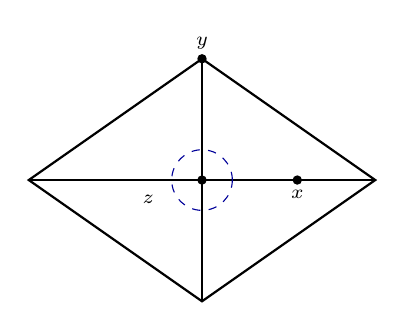
\begin{tikzpicture}[scale=1.1]
\draw[thick] (-2,0)--(0,1.4)--(2,0)--(0,-1.4)--cycle;
\draw[thick] (-2,0)--(2,0); \draw[thick] (0,1.4)--(0,-1.4);
\node[pt] at (0,1.4){}; \node[above] at (0,1.4){\scriptsize $y$};
\node[pt] at (0,0){}; \node at (-0.62,-0.22){\scriptsize $z$};
\node[pt] at (1.1,0){}; \node[below] at (1.1,0){\scriptsize $x$};
\draw[blue!60!black,dashed] (0,0) circle (0.35);
\end{tikzpicture}
\figtit{Figura 20. GT Ej.\ 4.3.4. Órdenes de corte locales: $x$ tiene $2$, $y$ tiene $3$, $z$ tiene $4$. Un entorno chico de $z$ (círculo rayado) menos $z$ se parte en $4$ trocitos de segmento; ninguno de los tres puntos es de corte global.}
\end{figure}

\begin{proposicion}[Invarianza de los puntos de corte locales \fnt{GT 4.3.5(b), pp.\,77--78} \noentra{todavía no dictado en clase}]
Si $f:X\to Y$ es un homeomorfismo, $x$ es de corte local de orden $n$ en $X$ si y sólo si $f(x)$ lo es en $Y$.
\lgc{f\ \text{homeomorfismo}\ \Rightarrow\ \big(x\ \text{de corte local de orden } n \text{ en } X\iff f(x)\ \text{de corte local de orden } n \text{ en } Y\big).}
\end{proposicion}

\begin{proof}[Idea]
Un homeomorfismo lleva entornos de $x$ en entornos de $f(x)$ y viceversa (es abierto y continuo), y restringido a $N'-\{x\}$ es un homeomorfismo sobre $f(N')-\{f(x)\}$; se aplica la Prop.~\ref{cc:invcam}.
\end{proof}

\subsection{Conexo más localmente arcoconexo implica arcoconexo}\label{cc:conexarco}

\noindent\noentra{todavía no dictado en clase} \textbf{GT} 4.4.5--4.4.6 y \textbf{MS} Prop.\ 7.18: la conexión es más débil que la arcoconexión, pero con una hipótesis local se recupera la equivalencia.

\begin{ejemplo}[Conexo que no es arcoconexo \fnt{GT Ej.\ 4.4.5, p.\,79; MS Ej.\ 7.2, p.\,91} \noentra{todavía no dictado en clase}]
La escalera (Ejemplo~\ref{cc:escalera}), el peine reducido (Ejemplos~\ref{ej:peine} y~\ref{cc:peinered}) y la curva seno del topólogo son conexos y no arcoconexos. Así, la Prop.~\ref{cc:arcoconexo} no tiene recíproca.
\end{ejemplo}

\begin{teorema}[Conexo y localmente arcoconexo $\Rightarrow$ arcoconexo \fnt{GT 4.4.6, p.\,79; MS Prop.\ 7.18, p.\,91} \noentra{todavía no dictado en clase}]\label{cc:conexlocarco}
Si $(X,\tp)$ es localmente conexo por caminos, entonces $X$ es conexo si y sólo si es conexo por caminos.
\lgc{X\ \text{loc.\ arcoconexo}\ \Rightarrow\ \big(X\ \text{conexo}\iff X\ \text{arcoconexo}\big).}
\end{teorema}

\begin{proof}
($\Leftarrow$) Es la Prop.~\ref{cc:arcoconexo}, que no usa la hipótesis local.
($\Rightarrow$) Si $X=\emptyset$ no hay nada que probar. Si no, sea $x_0\in X$. Por la Prop.~\ref{cc:compabcam}, $c(x_0)$ es abierta y cerrada, y no es vacía; como $X$ es conexo, $c(x_0)=X$ (Prop.~\ref{pr:conexclopen}). Es decir, todo punto se une con $x_0$ por un camino, y por transitividad (Prop.~\ref{cc:equiv}) dos puntos cualesquiera se unen entre sí.
\end{proof}

\begin{corolario}[Abiertos conexos de $\R^n$ \fnt{MS Ejemplos 7.3(4), p.\,91} \noentra{todavía no dictado en clase}]\label{cc:abiertosRn}
Todo abierto conexo de $\R^n$ (o de un espacio normado) es arcoconexo. De hecho, dos puntos se unen con una poligonal.
\lgc{U\subseteq\R^n\ \text{abierto}\ \wedge\ U\ \text{conexo}\ \Rightarrow\ U\ \text{arcoconexo}.}
\end{corolario}

\begin{proof}
$U$ es localmente arcoconexo: las bolas contenidas en $U$ son convexas y forman bases de entornos (Ejemplo~\ref{cc:ejlocarco}). Se aplica el Teorema~\ref{cc:conexlocarco}. (Para la poligonal: el conjunto de puntos que se unen con $x_0$ por una poligonal dentro de $U$ es abierto y cerrado en $U$, con el mismo argumento de la Prop.~\ref{cc:compabcam}.)
\end{proof}

\subsection{Componentes conexas y conexión local}\label{cc:compconex}

\noindent\noentra{todavía no dictado en clase} Sigue \textbf{GT} \S4.6 y \textbf{MS} \S7.2. Es la misma construcción que la de las componentes arcoconexas, con ``conexo'' en lugar de ``arcoconexo''; la diferencia importante es que ahora las componentes \emph{siempre} son cerradas (el sándwich sí vale para conexos).

\begin{definicion}[Componente conexa \fnt{GT 4.6.1, p.\,84; MS Def.\ 7.5, p.\,90} \noentra{todavía no dictado en clase}]\label{cc:defcomp}
Sea $(X,\tp)$ y $x\in X$. La \emph{componente conexa} de $x$, $C(x)$, es el mayor subconjunto conexo de $X$ que contiene a $x$: es conexo, contiene a $x$, y contiene a todo conexo que contenga a $x$.
\lgc{C(x)\ \text{conexo}\ \wedge\ x\in C(x)\ \wedge\ \forall A\subseteq X\ \big(A\ \text{conexo}\ \wedge\ x\in A\Rightarrow A\subseteq C(x)\big).}
\end{definicion}

\begin{lema}[La componente existe \fnt{GT Lema 4.6.2, p.\,84} \noentra{todavía no dictado en clase}]\label{cc:existecomp}
Para todo $x\in X$, $C(x)$ existe: es la unión de todos los conexos de $X$ que contienen a $x$.
\lgc{C(x)=\bigcup\{A\subseteq X:\ A\ \text{conexo},\ x\in A\}.}
\end{lema}

\begin{proof}
La familia no es vacía ($\{x\}$ es conexo) y todos sus miembros contienen a $x$, así que su unión es conexa (Prop.~\ref{pr:familias}(b)); contiene a $x$ y a cada conexo que contenga a $x$.
\end{proof}

\begin{proposicion}[Propiedades de las componentes conexas \fnt{GT 4.6.5 y Nota 4.6.4, pp.\,84--85; MS Lema 7.13, Teo.\ 7.14, Prop.\ 7.15(i), p.\,90} \noentra{todavía no dictado en clase}]\label{cc:propcomp}
En $(X,\tp)$, para todos $x,y\in X$:
\begin{enumerate}[label=(\arabic*),leftmargin=2.2em,itemsep=0pt]
\item $x\in C(x)$ y $C(x)$ es conexo;
\item $C(x)$ es \emph{cerrado} en $X$;
\item si $C(x)\cap C(y)\ne\emptyset$, entonces $C(x)=C(y)$: las componentes conexas forman una partición de $X$;
\item $X$ es conexo si y sólo si tiene una sola componente, $C(x)=X$ para todo $x$.
\end{enumerate}
\lgc{C(x)=\cl{C(x)};\qquad C(x)\cap C(y)\ne\emptyset\Rightarrow C(x)=C(y);\qquad X\ \text{conexo}\iff\forall x:\ C(x)=X.}
\end{proposicion}

\begin{proof}
(1) Por definición. (2) $\cl{C(x)}$ es conexo (sándwich, Prop.~\ref{pr:sandwich}) y contiene a $x$, así que $\cl{C(x)}\subseteq C(x)$ por maximalidad; la otra inclusión es de siempre. (3) $C(x)\cup C(y)$ es conexo por ser unión de conexos que se cortan (Prop.~\ref{pr:unionconex}) y contiene a $x$ y a $y$; por maximalidad $C(x)\cup C(y)\subseteq C(x)$ y $\subseteq C(y)$, luego $C(x)=C(y)$. (4) Si $X$ es conexo es él mismo el mayor conexo que contiene a $x$. Si $C(x)=X$, $X$ es conexo por (1).
\end{proof}

\begin{proposicion}[Un conexo queda dentro de una componente \fnt{MS Prop.\ 7.16, p.\,90; MS \S7.5, problema 9, p.\,93} \noentra{todavía no dictado en clase}]\label{cc:dentrocomp}
Si $C$ es una componente conexa de $X$ y $A\subseteq X$ es conexo, entonces $A\subseteq C$ o $A\cap C=\emptyset$. Además, todo subconjunto no vacío, conexo, abierto y cerrado de $X$ es una componente conexa.
\lgc{A\ \text{conexo}\Rightarrow A\subseteq C\ \vee\ A\subseteq X-C;\qquad \emptyset\ne A\ \text{conexo, abierto y cerrado}\Rightarrow A=C(a)\ \ \forall a\in A.}
\end{proposicion}

\begin{proof}
Si $A$ corta a $C=C(x)$ en $a$, entonces $C(a)=C$ y $A\subseteq C(a)$ por maximalidad. Para la segunda: si $a\in A$, $A\subseteq C(a)$ por maximalidad; y como $C(a)$ es conexo y corta al abierto-cerrado $A$, queda entero de ese lado (Prop.~\ref{pr:conexlado}): $C(a)\subseteq A$.
\end{proof}

\begin{proposicion}[Componentes arcoconexas dentro de componentes conexas \fnt{MS \S7.4, p.\,92 (``Def.'' 7.10)} \noentra{todavía no dictado en clase}]\label{cc:cenC}
Para todo $x\in X$, $c(x)\subseteq C(x)$: cada componente conexa es unión de componentes arcoconexas. En particular, un abierto-cerrado es unión de componentes arcoconexas (\textbf{CX} 17).
\lgc{\forall x\in X:\ c(x)\subseteq C(x);\qquad A\ \text{abierto y cerrado}\ \Rightarrow\ A=\bigcup_{a\in A}c(a).}
\end{proposicion}

\begin{proof}
$c(x)$ es arcoconexo, luego conexo (Prop.~\ref{cc:arcoconexo}), y contiene a $x$: por maximalidad $c(x)\subseteq C(x)$. Para \textbf{CX} 17: si $a\in A$, el conexo $c(a)$ corta al abierto-cerrado $A$, así que $c(a)\subseteq A$ (Prop.~\ref{pr:conexlado}).
\end{proof}

\begin{observacion}
\textbf{MS} numera este hecho como ``Definición 7.10'', pero es una afirmación demostrable. La inclusión puede ser estricta: en el peine reducido, $C(p)=R$ y $c(p)=\{p\}$.
\end{observacion}

\begin{proposicion}[Componentes e imagen continua \fnt{GT 4.6.10, p.\,87; MS \S7.5, problema 8, p.\,93; CX 20} \noentra{todavía no dictado en clase}]\label{cc:invcomp}
Sea $f:X\to Y$ continua. Entonces $f(C(x))\subseteq C(f(x))$, y si $E$ es una componente conexa de $Y$, $f^{-1}(E)$ es unión de componentes conexas de $X$. Si $f$ es un homeomorfismo, $f(C(x))=C(f(x))$ y $f$ induce una biyección entre las componentes conexas de $X$ y las de $Y$, con componentes correspondientes homeomorfas.
\lgc{f\ \text{continua}\Rightarrow f(C(x))\subseteq C(f(x))\ \wedge\ f^{-1}(E)=\bigcup_{x\in f^{-1}(E)}C(x);\qquad f\ \text{homeomorfismo}\Rightarrow f(C(x))=C(f(x)).}
\end{proposicion}

\begin{proof}
$f(C(x))$ es conexo (Prop.~\ref{pr:imconex}) y contiene a $f(x)$, así que está en $C(f(x))$. Si $x\in f^{-1}(E)$, entonces $E=C(f(x))\supseteq f(C(x))$, o sea $C(x)\subseteq f^{-1}(E)$ (\textbf{CX} 20). Para el homeomorfismo, igual que en la Prop.~\ref{cc:invcam}, aplicando lo anterior a $f^{-1}$; y la restricción de un homeomorfismo a $C(x)$ es un homeomorfismo sobre su imagen $C(f(x))$.
\end{proof}

\begin{ejemplo}[Componentes conexas \fnt{GT Ej.\ 4.6.3 y 4.6.6, pp.\,84--85; GT Ej.\ 4.6.9(2), p.\,86} \noentra{todavía no dictado en clase}]\label{cc:ejcomp}
\begin{lista}
\item En $\Q$ (usual) la componente de cada $x$ es $\{x\}$: los únicos conexos no vacíos son los puntos (es totalmente disconexo). Lo mismo en un discreto. Aquí las componentes \emph{no} son abiertas.
\item Sea $A=\{1/n: n\ge1\}\cup\{0\}$ y $X=A\times\R\subseteq\R^2$. La componente de $(a,y)$ es la recta $\{a\}\times\R$. En efecto, esa recta es conexa, luego está en la componente; y si $(a',y')\in C((a,y))$, la proyección $\pi_1(C((a,y)))$ es un conexo de $A\subseteq\Q$, luego un punto, que tiene que ser $a$: $a'=a$. La componente $\{0\}\times\R$ es cerrada pero no abierta en $X$.
\item En el peine reducido y en la escalera hay una sola componente conexa (son conexos), pero dos componentes arcoconexas.
\end{lista}
\end{ejemplo}

\begin{definicion}[Localmente conexo \fnt{GT 4.6.7, p.\,85} \noentra{todavía no dictado en clase}]\label{cc:deflocconex}
$(X,\tp)$ es \emph{localmente conexo} si todo entorno de cualquier punto contiene un entorno conexo de ese punto (cada punto tiene una base de entornos conexos).
\lgc{X\ \text{loc.\ conexo}\iff \forall x\in X\ \forall N\in\mathcal N_x\ \exists N'\in\mathcal N_x:\ N'\subseteq N\ \wedge\ N'\ \text{conexo}.}
\end{definicion}

\begin{observacion}
Localmente arcoconexo $\Rightarrow$ localmente conexo, porque los entornos arcoconexos son conexos (Prop.~\ref{cc:arcoconexo}). Ser conexo y ser localmente conexo son independientes (tabla de abajo).
\end{observacion}

\begin{proposicion}[En un localmente conexo las componentes son abiertas \fnt{GT 4.6.8, pp.\,85--86} \noentra{todavía no dictado en clase}]\label{cc:compab}
Si $(X,\tp)$ es localmente conexo, toda componente conexa $C(x)$ es abierta (y, por la Prop.~\ref{cc:propcomp}, abierta y cerrada).
\lgc{X\ \text{loc.\ conexo}\ \Rightarrow\ \forall x\in X:\ C(x)\in\tp.}
\end{proposicion}

\begin{proof}
Sea $y\in C(x)$, de modo que $C(y)=C(x)$. Aplicando la definición al entorno $N=X$, hay un entorno conexo $N'$ de $y$; como contiene a $y$, $N'\subseteq C(y)=C(x)$. Así $C(x)$ es entorno de cada uno de sus puntos.
\end{proof}

\begin{corolario}[Si hay un número finito de componentes, son abiertas \fnt{CX 23} \noentra{todavía no dictado en clase}]\label{cc:finitas}
Si $X$ tiene una cantidad finita de componentes conexas, cada una es abierta (y cerrada).
\lgc{X=C_1\cup\dots\cup C_k\ \text{(componentes)}\ \Rightarrow\ \forall i:\ C_i\in\tp.}
\end{corolario}

\begin{proof}
$X-C_i$ es la unión de las otras $k-1$ componentes, cada una cerrada (Prop.~\ref{cc:propcomp}); unión finita de cerrados es cerrada, así que $C_i$ es abierta.
\end{proof}

\begin{observacion}[Uso en la guía]
\textbf{CX} 21 (en un compacto con componentes abiertas hay finitas) usa la Prop.~\ref{cc:propcomp}(3): las componentes son un cubrimiento por abiertos disjuntos, del que no se puede sacar ninguno; necesita compacidad, que se ve más adelante. \textbf{CX} 22 (un abierto $U$ de un localmente conexo es localmente conexo) sale de que, si $U$ es abierto, los entornos de $x$ en el subespacio $U$ son exactamente los entornos de $x$ en $X$ contenidos en $U$.
\end{observacion}

\begin{corolario}[En un localmente arcoconexo, componentes conexas y arcoconexas coinciden \fnt{consecuencia de GT 4.2.6 y MS \S7.4, p.\,92} \noentra{todavía no dictado en clase}]\label{cc:igualcomp}
Si $X$ es localmente conexo por caminos, entonces $c(x)=C(x)$ para todo $x$.
\lgc{X\ \text{loc.\ arcoconexo}\ \Rightarrow\ \forall x\in X:\ c(x)=C(x).}
\end{corolario}

\begin{proof}
$c(x)\subseteq C(x)$ siempre (Prop.~\ref{cc:cenC}). Por la Prop.~\ref{cc:compabcam}, $c(x)$ es abierta y cerrada; el conexo $C(x)$ la corta (en $x$), así que $C(x)\subseteq c(x)$ (Prop.~\ref{pr:conexlado}).
\end{proof}

\begin{ejemplo}[Conexión local \fnt{GT Ej.\ 4.6.9, pp.\,86--87} \noentra{todavía no dictado en clase}]\label{cc:ejlocconex}
\begin{lista}
\item $\R^n$ es localmente arcoconexo, luego localmente conexo.
\item $(\R,\text{discreta})$ no es conexo pero sí localmente conexo ($\{x\}$ es un entorno conexo de $x$); sus componentes son los puntos, que acá sí son abiertos.
\item $\Q$ no es conexo ni localmente conexo: sus únicos conexos no vacíos son puntos, que no son entornos de nadie (tienen interior vacío).
\item El espacio del Ejemplo~\ref{cc:peinecompleto} (y el peine $P$) es conexo, incluso arcoconexo, y no es localmente conexo.
\end{lista}
\end{ejemplo}

\begin{ejemplo}[Aplicación: dos subespacios de $\R$ no homeomorfos \fnt{CX 19} \noentra{todavía no dictado en clase}]\label{cc:cx19}
$X=\N\cup\bigcup_{n\in\N}(-n-1,-n)$ e $Y=\N\cup[\frac12,\frac23]\cup\bigcup_{n\in\N}(-n-1,-n)$ no son homeomorfos (con $\N=\{1,2,\dots\}$). Los conexos de un subconjunto de $\R$ son intervalos (\S\ref{sec:bolzano}), así que las componentes conexas de $X$ son los puntos de $\N$ y los intervalos abiertos $(-n-1,-n)$; las de $Y$ son esas y además $[\frac12,\frac23]$. Contar componentes no alcanza (hay infinitas numerables en los dos), pero si $h:Y\to X$ fuera homeomorfismo, $h$ llevaría la componente $[\frac12,\frac23]$ sobre una componente de $X$ homeomorfa a ella (Prop.~\ref{cc:invcomp}): no puede ser un punto, y tampoco un intervalo abierto, porque $[\frac12,\frac23]$ tiene dos puntos que no son de corte y un intervalo abierto ninguno (Prop.~\ref{cc:invcorte}). (Si se toma $0\in\N$, en $X$ e $Y$ aparece además la componente $(-1,0]$, que tiene un solo punto que no es de corte; el argumento no cambia.)
\end{ejemplo}

\begin{observacion}[Mapa de ejemplos]
Resumen de las cuatro propiedades en los ejemplos de esta sección (``loc.''$=$localmente). Las implicaciones generales son: arcoconexo $\Rightarrow$ conexo; loc.\ arcoconexo $\Rightarrow$ loc.\ conexo; conexo $+$ loc.\ arcoconexo $\Rightarrow$ arcoconexo.
\begin{center}\small
\begin{tabular}{@{}lcccc@{}}
\hline
Espacio & conexo & arcoconexo & loc.\ conexo & loc.\ arcoconexo\\
\hline
$\R^n$, bolas, $S^1$, abiertos conexos de $\R^n$ & sí & sí & sí & sí\\
$[-1,0)\cup(0,1]$; $(\R,\text{discreta})$ & no & no & sí & sí\\
$\Q$ & no & no & no & no\\
peine $P$; Ej.~\ref{cc:peinecompleto}; \textbf{CX} 15 & sí & sí & no & no\\
peine reducido $R$; escalera; seno del topólogo & sí & no & no & no\\
\hline
\end{tabular}
\end{center}
Falta en la tabla ``conexo, localmente conexo y no arcoconexo'': por el Teorema~\ref{cc:conexlocarco} un ejemplo así no puede ser localmente arcoconexo. Existe: $\N$ con la topología cofinita es conexo y localmente conexo (todo abierto no vacío es infinito con la cofinita, luego conexo, Ej.~\ref{ej:conex}), pero no es arcoconexo; esto último usa un teorema de Sierpi\'nski ($[0,1]$ no es unión numerable de dos o más cerrados no vacíos disjuntos dos a dos), que excede el curso.
\end{observacion}


\subsection{Intervalos de $\R$ y Bolzano}\label{sec:bolzano}

\noindent La docente lo dejó para más adelante (\textbf{GT} 4.4.4 y 4.5.1, junto con los postergados 2.7.6 y 2.8.3 de \S\ref{sec:sub}). Van acá con las demostraciones completas, para tenerlas listas cuando se dicten. El orden es: primero $[a,b]$ es conexo (el único lugar donde se usa algo de $\R$: el axioma del supremo), después todos los intervalos, después la caracterización de los conexos de la recta y, por último, Bolzano.

\begin{definicion}[Intervalo \fnt{curso; GT 2.7.6 y 4.4.4, pp.\,33 y 79 (``intervalo de cualquier tipo'')} \noentra{todavía no dictado en clase}]
$J\subseteq\R$ es un \emph{intervalo} si es de alguna de las formas $(\alpha,\beta)$, $[\alpha,\beta)$, $(\alpha,\beta]$, $[\alpha,\beta]$ con $-\infty\le\alpha\le\beta\le+\infty$, sin corchete en un extremo infinito. Incluye a $\emptyset$, a los unitarios $[a,a]$, a las semirrectas y a $\R=(-\infty,+\infty)$. Todos cumplen que si contienen a dos puntos contienen a todo el segmento entre ellos.
\lgc{J\ \text{intervalo}\ \Rightarrow\ \forall a,b\in J\ \big(a\le b\Rightarrow[a,b]\subseteq J\big).}
\end{definicion}

\begin{teorema}[{$[a,b]$ es conexo \fnt{GT 2.7.6, p.\,33, para $J=[a,b]$; MS Ejemplos 7.1(11), p.\,88} \noentra{todavía no dictado en clase}}]\label{hu:abconex}
Si $a\le b$, el intervalo cerrado $[a,b]$ con la topología usual es conexo: sus únicos subconjuntos abiertos y cerrados a la vez son $\emptyset$ y $[a,b]$.
\lgc{a\le b\ \wedge\ C\subseteq[a,b]\ \text{abierto y cerrado en } [a,b]\ \Rightarrow\ C=\emptyset\ \vee\ C=[a,b].}
\end{teorema}

\begin{proof}
Si $a=b$ es un punto. Sea $a<b$ y sea $C$ abierto y cerrado en $[a,b]$. Alcanza con probar:
\[
(\ast)\qquad a\in C\ \Longrightarrow\ C=[a,b].
\]
En efecto, si $a\in C$, $(\ast)$ da $C=[a,b]$; si $a\notin C$, entonces $[a,b]-C$ también es abierto y cerrado en $[a,b]$ y contiene a $a$, así que $(\ast)$ da $[a,b]-C=[a,b]$, o sea $C=\emptyset$. Por la Prop.~\ref{pr:conexclopen}, $[a,b]$ es conexo.

\emph{Prueba de $(\ast)$.} Se considera el conjunto de los $t$ hasta los cuales $C$ llega ``sin cortes'':
\[
S=\{t\in[a,b]:\ [a,t]\subseteq C\}.
\]
$S\ne\emptyset$ porque $a\in S$ (es $[a,a]=\{a\}\subseteq C$), y $S$ está acotado por $b$. Por el axioma del supremo existe $s=\sup S$, y $a\le s\le b$.

\emph{Paso 1: $[a,s)\subseteq C$.} Si $a\le u<s$, como $u$ no es cota superior de $S$ hay $t\in S$ con $u<t$; entonces $u\in[a,t]\subseteq C$.

\emph{Paso 2: $s\in C$, luego $s\in S$ (uso de ``cerrado'').} Cada $t\in S$ está en $C$ (porque $t\in[a,t]\subseteq C$), o sea $S\subseteq C$. Por la Prop.~\ref{hu:supadh}, el supremo es adherente: $s\in\cl S\subseteq\cl C$ (clausuras en $\R$). Como $s\in[a,b]$, resulta $s\in\cl C\cap[a,b]=\cl C^{\,[a,b]}$ (Prop.~\ref{pr:subesp}(iv)), que es $C$ porque $C$ es cerrado en $[a,b]$. Con el paso 1, $[a,s]\subseteq C$, es decir $s\in S$.

\emph{Paso 3: $s=b$ (uso de ``abierto'').} Supongamos $s<b$. Como $C$ es abierto en $[a,b]$, es $C=G\cap[a,b]$ con $G$ abierto de $\R$; como $s\in G$, hay $\delta>0$ con $(s-\delta,s+\delta)\subseteq G$, luego $(s-\delta,s+\delta)\cap[a,b]\subseteq C$. Sea $s'=\min\{s+\delta/2,\,b\}$; es $s<s'\le b$ y $(s,s']\subseteq(s-\delta,s+\delta)\cap[a,b]\subseteq C$. Junto con el paso 2, $[a,s']=[a,s]\cup(s,s']\subseteq C$, o sea $s'\in S$ con $s'>s=\sup S$. Absurdo.

Por los pasos 2 y 3, $b=s\in S$, es decir $[a,b]\subseteq C$, y $C=[a,b]$.
\end{proof}

\begin{figure}[ht]
\centering
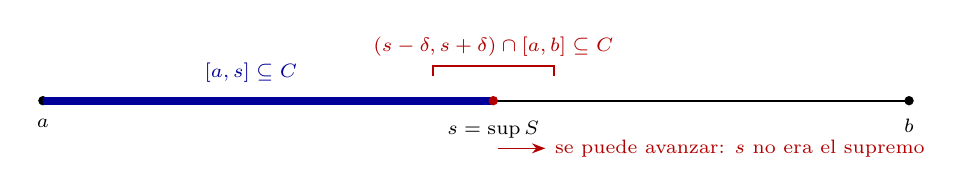
\begin{tikzpicture}[scale=1.1]
\draw[thick] (0,0)--(10,0);
\node[pt] at (0,0) {}; \node[below] at (0,-0.1) {\scriptsize $a$};
\node[pt] at (10,0) {}; \node[below] at (10,-0.1) {\scriptsize $b$};
\draw[blue!60!black,line width=3pt] (0,0)--(5.2,0);
\node[pt,fill=red!70!black] at (5.2,0) {}; \node[below] at (5.2,-0.12) {\scriptsize $s=\sup S$};
\draw[red!70!black,thick] (4.5,0.28)--(4.5,0.4)--(5.9,0.4)--(5.9,0.28);
\node[red!70!black,above] at (5.2,0.4) {\scriptsize $(s-\delta,s+\delta)\cap[a,b]\subseteq C$};
\node[blue!60!black,above] at (2.4,0.1) {\scriptsize $[a,s]\subseteq C$};
\draw[->,>=Stealth,red!70!black] (5.25,-0.55)--(5.8,-0.55) node[right]{\scriptsize se puede avanzar: $s$ no era el supremo};
\end{tikzpicture}
\figtit{Figura 21. La prueba por supremo. ``Cerrado'' asegura que $C$ contiene al punto $s$ al que llega; ``abierto'' asegura que, si $s<b$, desde $s$ se puede seguir un poco más. Las dos cosas juntas sólo son compatibles con $s=b$.}
\end{figure}

\begin{intuicion}
Es la versión rigurosa de ``para salir de $C$ habría que saltar'': se avanza desde $a$ tanto como se pueda sin salir de $C$; el punto al que se llega no puede ser un borde de $C$ ni por la izquierda (porque $C$ es cerrado) ni por la derecha (porque $C$ es abierto). Lo único de $\R$ que se usa es que todo conjunto no vacío y acotado tiene supremo: en $\Q$ la misma prueba falla, y de hecho $\Q$ es totalmente disconexo.
\end{intuicion}

\begin{corolario}[Todo intervalo es conexo; en particular $\R$ \fnt{GT 2.7.6, p.\,33} \noentra{todavía no dictado en clase}]\label{hu:intconex}
Todo intervalo $J\subseteq\R$ (de cualquier tipo, incluida la recta) es conexo: sus únicos abiertos y cerrados relativos son $\emptyset$ y $J$. En particular $(\R,\tp_u)$ es conexo, y quedan justificados los usos de ``$\R$ es conexo'' de \S\ref{sec:conex}.
\lgc{J\subseteq\R\ \text{intervalo}\ \Rightarrow\ J\ \text{conexo};\qquad (\R,\tp_u)\ \text{conexo}.}
\end{corolario}

\begin{proof}
Dados $x\le y$ en $J$, el segmento $[x,y]$ está contenido en $J$ y es conexo (Teo.~\ref{hu:abconex}). Por la Prop.~\ref{pr:dospuntos} (versión para subconjuntos), $J$ es conexo.
\end{proof}

\begin{observacion}[La demostración de GT 2.7.6 y sus erratas]
\textbf{GT} prueba el corolario directamente para $J$, con la misma idea: elige $t_0\in J-A$, toma $A_0=A\cap(-\infty,t_0)$ y su supremo $a$, y usa el Ej.\ 2.3.7 (acá Prop.~\ref{hu:supadh}) y la Nota 2.7.4 para ver que $a\in A_0$. Hay tres descuidos: escribe $(\infty,t_0)$ por $(-\infty,t_0)$; el entorno que usa al final es $\{t\in J: |t-t_0|<\delta\}$, cuando debe ser alrededor de $a$, $\{t\in J:|t-a|<\delta\}\subseteq A_0$ (con $\delta\le t_0-a$); y sólo trata el caso $A_0\ne\emptyset$ (si $A_0=\emptyset$ se hace lo mismo con $A_1=A\cap(t_0,\infty)$ y su ínfimo). La prueba de arriba evita esos casos pasando por $[a,b]$.
\end{observacion}

\begin{proposicion}[Los conexos de la recta \fnt{GT 4.4.4, p.\,79 y 4.1.5, pp.\,62--63; MS Ejemplos 7.1(11), p.\,88} \noentra{todavía no dictado en clase}]\label{hu:conexR}
Para $A\subseteq(\R,\tp_u)$ son equivalentes:
\begin{enumerate}[label=(\arabic*),leftmargin=2.2em,itemsep=0pt]
\item $A$ es conexo por caminos: para todos $x,y\in A$ hay un \emph{camino} en $A$ de $x$ a $y$, es decir, una $\gamma:[0,1]\to A$ continua con $\gamma(0)=x$, $\gamma(1)=y$ \fnt{GT Defs.\ 4.1.1--4.1.2, p.\,61};
\item $A$ es conexo;
\item si $a\le b$ están en $A$, entonces $[a,b]\subseteq A$;
\item $A$ es un intervalo.
\end{enumerate}
\lgc{A\subseteq\R:\quad A\ \text{conexo por caminos}\iff A\ \text{conexo}\\ \iff \forall a,b\in A\ \big(a\le b\Rightarrow[a,b]\subseteq A\big)\iff A\ \text{intervalo}.}
\end{proposicion}

\begin{proof}
(1)$\Rightarrow$(2): dados $x,y\in A$, la imagen $\gamma([0,1])$ de un camino entre ellos es conexa (imagen continua del conexo $[0,1]$, Prop.~\ref{pr:imconex} y Teo.~\ref{hu:abconex}), está contenida en $A$ y contiene a $x$ e $y$. Por la Prop.~\ref{pr:dospuntos}, $A$ es conexo.

(2)$\Rightarrow$(3), por el contrarrecíproco: si $a<t<b$ con $a,b\in A$ y $t\notin A$, los abiertos $G=(-\infty,t)$ y $H=(t,+\infty)$ de $\R$ cumplen $a\in G\cap A$, $b\in H\cap A$, $G\cap H=\emptyset$ y $A\subseteq G\cup H$ (porque $t\notin A$). Por la Prop.~\ref{pr:GH}, $A$ no es conexo.

(3)$\Rightarrow$(4): si $A=\emptyset$ es un intervalo. Si no, sean $\alpha=\inf A\in[-\infty,+\infty)$ y $\beta=\sup A\in(-\infty,+\infty]$ (valen $\mp\infty$ si $A$ no está acotado de ese lado). Si $\alpha<t<\beta$, como $t$ no es cota inferior ni superior de $A$, hay $a,b\in A$ con $a<t<b$, y por (3) $t\in[a,b]\subseteq A$. Así $(\alpha,\beta)\subseteq A\subseteq[\alpha,\beta]\cap\R$, y $A$ es $(\alpha,\beta)$ con o sin cada extremo finito: un intervalo.

(4)$\Rightarrow$(1): dados $x\le y$ en el intervalo $A$, $\gamma(t)=(1-t)x+ty$ es continua, $\gamma(0)=x$, $\gamma(1)=y$, y toma valores en $[x,y]\subseteq A$ \fnt{GT Ej.\ 4.1.3(1), p.\,61}. (Para $x>y$ se usa el camino recorrido al revés.)
\end{proof}

\begin{observacion}
La implicación (2)$\Rightarrow$(3) es la que más se usa en los ejercicios, casi siempre en su forma contrarrecíproca: \emph{si a un subconjunto de $\R$ le falta un punto entre dos de los suyos, se desconecta cortando en ese punto}. Por ejemplo, $\Q$, $\R-\{0\}$ y $[0,1]\cup[2,3]$ no son conexos.
\end{observacion}

\begin{teorema}[Bolzano \fnt{GT 2.8.3, p.\,35 $=$ GT 4.5.1, p.\,80} \noentra{todavía no dictado en clase}]\label{hu:bolzano}
Para un espacio topológico $(X,\tp)$ son equivalentes:
\begin{enumerate}[label=(\alph*),leftmargin=2.2em,itemsep=0pt]
\item $X$ es conexo, es decir (Prop.~\ref{pr:conexclopen}), sus únicos abiertos y cerrados son $\emptyset$ y $X$;
\item (valor intermedio) si $f:X\to\R$ es continua y $a\le b$ son valores de $f$, entonces $f$ toma todos los valores entre $a$ y $b$;
\item (Bolzano) si $f:X\to\R$ es continua y toma un valor negativo y uno positivo, entonces se anula en algún punto.
\end{enumerate}
\lgc{X\ \text{conexo}\iff \big[\forall f:X\to\R\ \text{continua}:\ a,b\in f(X)\ \wedge\ a\le b\ \Rightarrow\ [a,b]\subseteq f(X)\big]\\
\iff \big[\forall f:X\to\R\ \text{continua}:\ \exists x_1,x_2\ f(x_1)<0<f(x_2)\ \Rightarrow\ \exists x_0\ f(x_0)=0\big].}
\end{teorema}

\begin{proof}
(a)$\Rightarrow$(b), por el absurdo. Sean $a=f(x_1)<b=f(x_2)$ (si $a=b$ no hay nada que probar) y supongamos que hay $t\in(a,b)$ con $t\notin f(X)$. Sea $A=f^{-1}\big((t,+\infty)\big)$. Es abierto porque $f$ es continua. Como $f$ no toma el valor $t$, también $A=f^{-1}\big([t,+\infty)\big)$, que es cerrado (preimagen de un cerrado). Además $x_2\in A$ porque $f(x_2)=b>t$, y $x_1\notin A$ porque $f(x_1)=a<t$. Entonces $A$ es abierto y cerrado, con $A\ne\emptyset$ y $A\ne X$: contradice (a).

(b)$\Rightarrow$(c): si $f(x_1)<0<f(x_2)$, por (b) con $a=f(x_1)$ y $b=f(x_2)$ es $0\in[a,b]\subseteq f(X)$, o sea $f(x_0)=0$ para algún $x_0$.

(c)$\Rightarrow$(a), por el contrarrecíproco. Si $A\ne\emptyset,X$ es abierto y cerrado, sea $f=1$ en $A$ y $f=-1$ en $X-A$. Es continua: la preimagen de cualquier $G\subseteq\R$ es $\emptyset$, $A$, $X-A$ o $X$ según cuáles de $\pm1$ estén en $G$, y los cuatro son abiertos. Toma el valor $-1<0$ (en $X-A\ne\emptyset$) y el valor $1>0$ (en $A\ne\emptyset$), pero no se anula: falla (c).
\end{proof}

\begin{observacion}[Otra prueba de (a)$\Rightarrow$(b)]
Con lo de esta sección sale en una línea: $f(X)$ es conexo (imagen continua de un conexo, Prop.~\ref{pr:imconex}), luego es un intervalo (Prop.~\ref{hu:conexR}), luego contiene a $[a,b]$ si contiene a $a$ y a $b$. La prueba de \textbf{GT} tiene la ventaja de no usar la caracterización de los conexos de $\R$, que en \textbf{GT} viene recién en el cap.~4.
\end{observacion}

\begin{corolario}[Bolzano y valor intermedio clásicos \fnt{GT 2.8.3, ``Consecuencia'', p.\,36} \noentra{todavía no dictado en clase}]\label{hu:tvi}
Sea $J\subseteq\R$ un intervalo y $f:J\to\R$ continua. Entonces $f(J)$ es un intervalo. En particular, si $f:[a,b]\to\R$ es continua y $f(a)<0<f(b)$ (o $f(a)>0>f(b)$), existe $c\in(a,b)$ con $f(c)=0$; y $f$ toma todos los valores entre $f(a)$ y $f(b)$.
\lgc{J\ \text{intervalo}\ \wedge\ f:J\to\R\ \text{continua}\ \Rightarrow\ f(J)\ \text{intervalo};\\
f:[a,b]\to\R\ \text{continua}\ \wedge\ f(a)\,f(b)<0\ \Rightarrow\ \exists c\in(a,b):\ f(c)=0.}
\end{corolario}

\begin{proof}
$J$ es conexo (Cor.~\ref{hu:intconex}), luego $f(J)$ es conexo (Prop.~\ref{pr:imconex}) y, por la Prop.~\ref{hu:conexR}, un intervalo. Para la segunda parte se aplica el Teorema~\ref{hu:bolzano}(c) a $X=[a,b]$ (a $-f$ si $f(a)>0>f(b)$); el cero no está en $a$ ni en $b$ porque ahí $f\ne0$.
\end{proof}

\begin{observacion}[Cómo se usa]
Para probar que una ecuación $g(x)=h(x)$ tiene solución en un intervalo, se aplica el corolario a $f=g-h$ y se buscan dos puntos con signos opuestos. Para probar que \emph{un espacio no es conexo}, alcanza con exhibir una continua a $\R$ que cambie de signo sin anularse; y para probar que \emph{dos espacios no son homeomorfos}, sirve comparar qué pasa al sacar un punto: $\R-\{0\}$ no es conexo (le falta el $0$ entre $-1$ y $1$), mientras que $\R^2-\{0\}$ sí lo es (unión de los rayos abiertos que salen del origen, todos cortando a la circunferencia unidad, Prop.~\ref{pr:familias}(a)). Como un homeomorfismo $f:\R\to\R^2$ se restringiría a un homeomorfismo entre $\R-\{0\}$ y $\R^2-\{f(0)\}$, resulta $\R\not\cong\R^2$.
\end{observacion}


%======================================================================
\section[Compacidad]{Compacidad \noentra{todavía no dictado en clase}}\label{sec:compac}

\noindent \textbf{Todo este capítulo está todavía no dictado en clase}: se incluye para tener el mapa completo, porque la docente anticipó que la topología producto se evalúa ``con conexidad o con compacidad''. Sigue \textbf{GT} cap.~3 (\S\S3.1--3.8, pp.\,44--60), cruzado con \textbf{MS} cap.~6 (pp.\,79--84). El producto de compactos se hace con la topología producto de \S\ref{sec:prod} (lema del tubo), no con la versión métrica de \textbf{GT} 3.5.1. En \textbf{GT} varios enunciados dicen ``(seudo)métrico''; acá se escriben para métricos, que es lo que usan los ejercicios (en un seudométrico se pierde Hausdorff y con él la \S\ref{cp:sub-t2}).

%----------------------------------------------------------------------
\subsection[Definición y primeros ejemplos]{Definición y primeros ejemplos \noentra{todavía no dictado en clase}}\label{cp:sub-def}

\begin{definicion}[Recubrimiento, subrecubrimiento \fnt{GT 3.1.1--3.1.3, p.\,44; MS Def.\ 6.1, p.\,79}]
Sea $X$ un conjunto y $A\subseteq X$. Un \emph{recubrimiento} de $A$ (en \textbf{MS}: \emph{cubrimiento}) es una familia $\{C_\alpha\}_{\alpha\in\Lambda}$ de subconjuntos de $X$ cuya unión contiene a $A$; si $A=X$, la unión es exactamente $X$. Es un \emph{recubrimiento por abiertos} si cada $C_\alpha$ es abierto. Un \emph{subrecubrimiento} es una subfamilia $\{C_\alpha\}_{\alpha\in\Lambda'}$, con $\Lambda'\subseteq\Lambda$, que todavía cubre a $A$; es \emph{finito} si $\Lambda'$ es finito.
\lgc{\{C_\alpha\}_{\alpha\in\Lambda}\ \text{recubre } A\iff A\subseteq\textstyle\bigcup_{\alpha\in\Lambda}C_\alpha;\\
\{C_\alpha\}_{\alpha\in\Lambda'}\ \text{subrecubrimiento}\iff \Lambda'\subseteq\Lambda\ \wedge\ A\subseteq\textstyle\bigcup_{\alpha\in\Lambda'}C_\alpha.}
\end{definicion}

\begin{definicion}[Compacto \fnt{GT 3.1.4--3.1.5, p.\,44; MS Def.\ 6.2, p.\,79}]\label{cp:def}
Sea $(X,\tp)$ un espacio topológico y $A\subseteq X$. $A$ es \emph{compacto} (en $(X,\tp)$) si de \emph{todo} recubrimiento de $A$ por abiertos de $X$ se puede extraer un subrecubrimiento finito. Si $A=X$, se dice que $(X,\tp)$ es un \emph{espacio compacto}.
\lgc{A\ \text{compacto}\iff \forall\{G_\alpha\}_{\alpha\in\Lambda}\subseteq\tp\ \Big(A\subseteq\textstyle\bigcup_{\alpha\in\Lambda}G_\alpha\\ \Rightarrow\ \exists\alpha_1,\dots,\alpha_n\in\Lambda:\ A\subseteq G_{\alpha_1}\cup\dots\cup G_{\alpha_n}\Big).}
\end{definicion}

\begin{intuicion}
El cuantificador es ``\emph{todo} recubrimiento'': para probar que algo es compacto hay que tomar un recubrimiento abierto \emph{cualquiera} (no uno elegido por uno) y achicarlo a finitos. Para probar que \emph{no} es compacto alcanza con exhibir \emph{un} recubrimiento abierto sin subrecubrimiento finito. Es la misma asimetría que en conexidad, pero dada vuelta: acá lo fácil es romper la compacidad. La imagen mental: un compacto es un conjunto que ``se comporta como si fuera finito'' respecto de los abiertos; los resultados de este capítulo son, casi todos, cosas obvias para conjuntos finitos que siguen valiendo para compactos.
\end{intuicion}

\begin{lema}[La compacidad es absoluta \fnt{GT 3.1.6, pp.\,44--45; MS Lema 6.1, pp.\,79--80}]\label{cp:absoluta}
Sea $A\subseteq(X,\tp)$. Entonces $A$ es compacto en $(X,\tp)$ si y sólo si el subespacio $(A,\tp_A)$ es un espacio compacto. En particular, si $A\subseteq B\subseteq X$, $A$ es compacto en $X$ sii es compacto en el subespacio $B$.
\lgc{A\ \text{compacto en } (X,\tp)\iff (A,\tp_A)\ \text{compacto}.}
\end{lema}

\begin{proof}
Se traducen los recubrimientos con $\tp_A=\{G\cap A: G\in\tp\}$. ($\Rightarrow$) Si $A=\bigcup_\alpha(H_\alpha\cap A)$ con $H_\alpha\in\tp$, los $H_\alpha$ recubren $A$ por abiertos de $X$; se extraen $H_{\alpha_1},\dots,H_{\alpha_n}$ y entonces $A=(H_{\alpha_1}\cap A)\cup\dots\cup(H_{\alpha_n}\cap A)$. ($\Leftarrow$) Si $A\subseteq\bigcup_\alpha U_\alpha$ con $U_\alpha\in\tp$, los $U_\alpha\cap A$ recubren al espacio $A$ por abiertos de $\tp_A$; se extraen finitos, $A=\bigcup_{i}(U_{\alpha_i}\cap A)\subseteq\bigcup_iU_{\alpha_i}$.
\end{proof}

\begin{observacion}
Por el lema, ``$A$ es compacto'' no depende del espacio ambiente (a diferencia de ``$A$ es abierto'', ver \S\ref{sec:sub}), y todo lo que se pruebe para espacios compactos vale para subconjuntos compactos. Además \textbf{MS} (Obs.\ 6.1(2), p.\,80) observa que en la definición alcanza con recubrimientos por abiertos \emph{básicos}: si $\{G_\alpha\}$ es un recubrimiento abierto, cada punto está en un básico metido en algún $G_\alpha$; se extrae un subrecubrimiento finito de esos básicos y se reemplaza cada uno por el $G_\alpha$ que lo contiene.
\end{observacion}

\begin{proposicion}[Finitos y uniones finitas \fnt{GT Ej.\ 3.1.9 y 3.1.11, p.\,45; MS Obs.\ 6.1(1),(4), p.\,80}]\label{cp:finitos}
En cualquier espacio topológico, todo conjunto finito es compacto, y la unión de una cantidad finita de compactos es compacta.
\lgc{A\ \text{finito}\Rightarrow A\ \text{compacto};\qquad A_1,\dots,A_m\ \text{compactos}\Rightarrow A_1\cup\dots\cup A_m\ \text{compacto}.}
\end{proposicion}

\begin{proof}
Si $A=\{a_1,\dots,a_s\}\subseteq\bigcup_\alpha G_\alpha$, para cada $a_i$ se elige un $G_{\alpha_i}\ni a_i$; los $s$ elegidos cubren $A$. Si $\{G_\alpha\}$ cubre $A_1\cup\dots\cup A_m$, cubre a cada $A_j$; cada uno usa finitos, y la unión de $m$ familias finitas es finita.
\end{proof}

\begin{ejemplo}[Espacios que no son compactos \fnt{GT Ej.\ 3.1.7, p.\,45; MS Ejemplos 6.1(8) y Contraej.\ 6.1, pp.\,80--81}]\label{cp:nocomp}
\begin{lista}
\item $(\R^n,\tp_u)$ no es compacto: $\R^n=\bigcup_{k\ge1}\Bola{0}{k}$, y una cantidad finita de esas bolas es la de radio máximo, que no es todo $\R^n$.
\item $(0,1)$ no es compacto: $\{(\tfrac1k,1)\}_{k\ge2}$ lo recubre, y finitos de ellos dan $(\tfrac1{k_0},1)\ne(0,1)$.
\end{lista}
\end{ejemplo}

\begin{ejemplo}[Las topologías de referencia \fnt{GT Ej.\ 3.1.8 y 3.1.10, p.\,45; MS Ejs.\ 6.1(1), (2), (5) y (6), p.\,80}]\label{cp:ejtop}
\begin{lista}
\item \emph{Indiscreta}: todo subconjunto es compacto (el único abierto no vacío es $X$, así que cualquier recubrimiento contiene a $X$).
\item \emph{Discreta}: $A$ es compacto sii es finito. Si $A$ es infinito, $\{\{a\}\}_{a\in A}$ es un recubrimiento abierto en el que ningún elemento sobra, luego no tiene subrecubrimiento finito. En particular, $(\N,\tp_{dis})$ y $(\R,d_D)$ no son compactos.
\item \emph{Cofinita}: $(X,\tp_{cof})$ es compacto, y de hecho todo subconjunto lo es. Dado un recubrimiento abierto de $A\ne\emptyset$, se toma un $G_{\alpha_0}$ no vacío que corte a $A$; su complemento $X-G_{\alpha_0}$ es finito, y los finitos puntos de $A$ que quedan afuera se cubren con un abierto cada uno.
\item \emph{Conumerable} sobre $\R$: sólo los finitos son compactos (\textbf{MS}).
\end{lista}
\end{ejemplo}

\begin{teorema}[Los intervalos cerrados y acotados son compactos \fnt{GT Ej.\ 3.1.12, p.\,46}]\label{cp:ab}
En $(\R,\tp_u)$, todo intervalo $[a,b]$ es compacto.
\lgc{a\le b\ \Rightarrow\ [a,b]\ \text{compacto en } (\R,\tp_u).}
\end{teorema}

\begin{proof}
Sea $\{G_\alpha\}$ un recubrimiento de $[a,b]$ por abiertos de $\R$, y sea
$S=\{x\in[a,b]:\ [a,x]\ \text{se cubre con finitos } G_\alpha\}$. $S\ne\emptyset$ porque $a\in S$ y está acotado por $b$; sea $x_0=\sup S\in[a,b]$. Como $x_0$ está en algún $G_{\alpha'}$ abierto, hay $\varepsilon>0$ con $(x_0-\varepsilon,x_0+\varepsilon)\subseteq G_{\alpha'}$.
\begin{lista}
\item $x_0\in S$: por ser supremo hay $x_1\in S$ con $x_0-\varepsilon<x_1\le x_0$; $[a,x_1]$ se cubre con $G_{\alpha_1},\dots,G_{\alpha_n}$ y $[x_1,x_0]\subseteq G_{\alpha'}$, así que $[a,x_0]$ se cubre con $n+1$ de ellos.
\item $x_0=b$: si fuera $x_0<b$, el mismo cubrimiento finito, agregando $G_{\alpha'}$, cubre $[a,x_0+\varepsilon_0/2]$ con $\varepsilon_0=\min\{\varepsilon,b-x_0\}$, y ese punto está en $S$ y es mayor que el supremo. Absurdo.
\end{lista}
Luego $b\in S$: $[a,b]$ se cubre con finitos $G_\alpha$.
\end{proof}

\begin{observacion}
La demostración usa el axioma del supremo de $\R$ y nada más: es la ``inducción continua'' que avanza por $[a,b]$ mientras se pueda cubrir con finitos. En $\Q$ el mismo argumento falla (el supremo puede no existir), y de hecho $[0,2]\cap\Q$ no es compacto en $\Q$ (Ej.~\ref{cp:ejlc}).
\end{observacion}

\begin{proposicion}[En un métrico, compacto implica acotado \fnt{GT 3.1.13, p.\,46}]\label{cp:acotado}
Sea $(X,d)$ un espacio métrico y $C\subseteq X$ compacto. Entonces $C$ es acotado.
\lgc{C\ \text{compacto en } (X,d)\ \Rightarrow\ \delta(C)<\infty.}
\end{proposicion}

\begin{proof}
Si $C=\emptyset$ no hay nada que probar. Si no, se fija $x_0\in C$: las bolas $\Bola{x_0}{n}$, $n\ge1$, cubren todo $X$, y en particular a $C$. Se extraen finitas; como están encajadas, $C\subseteq\Bola{x_0}{n_0}$ con $n_0$ el mayor radio. Por la desigualdad triangular, $d(x,x')\le d(x,x_0)+d(x_0,x')<2n_0$ para $x,x'\in C$.
\end{proof}

%----------------------------------------------------------------------
\subsection[Compacidad y cerrados]{Compacidad y cerrados \noentra{todavía no dictado en clase}}\label{cp:sub-cerr}

\begin{definicion}[Propiedad de intersección finita \fnt{GT 3.2.1, p.\,47; MS Def.\ 6.3, p.\,80}]
Una familia de conjuntos $\{A_\alpha\}_{\alpha\in\Lambda}$ tiene la \emph{propiedad de intersección finita} (PIF) si toda subfamilia finita tiene intersección no vacía.
\lgc{\{A_\alpha\}_{\alpha\in\Lambda}\ \text{tiene la PIF}\iff \forall\alpha_1,\dots,\alpha_n\in\Lambda:\ A_{\alpha_1}\cap\dots\cap A_{\alpha_n}\ne\emptyset.}
\end{definicion}

\begin{teorema}[Compacidad por cerrados \fnt{GT 3.2.2, p.\,47; MS Teo.\ 6.2, p.\,81}]\label{cp:pif}
$(X,\tp)$ es compacto si y sólo si toda familia de cerrados de $X$ con la PIF tiene intersección no vacía.
\lgc{X\ \text{compacto}\iff \forall\{F_\alpha\}_{\alpha\in\Lambda}\ \text{cerrados}:\ \big(\{F_\alpha\}\ \text{tiene la PIF}\Rightarrow \textstyle\bigcap_{\alpha\in\Lambda}F_\alpha\ne\emptyset\big).}
\end{teorema}

\begin{proof}
Es la definición pasada a complementos: $\{G_\alpha\}$ es un recubrimiento abierto de $X$ sii $\{X-G_\alpha\}$ es una familia de cerrados con intersección vacía, y $G_{\alpha_1}\cup\dots\cup G_{\alpha_n}=X$ sii $(X-G_{\alpha_1})\cap\dots\cap(X-G_{\alpha_n})=\emptyset$ (De Morgan). ($\Rightarrow$) Si $\{F_\alpha\}$ tiene la PIF y $\bigcap F_\alpha=\emptyset$, los $X-F_\alpha$ recubren $X$; por compacidad finitos lo hacen, y entonces finitos $F_\alpha$ tienen intersección vacía: contradice la PIF. ($\Leftarrow$) Si $\{G_\alpha\}$ recubre $X$, la familia $\{X-G_\alpha\}$ tiene intersección vacía, luego \emph{no} tiene la PIF: hay finitos con $\bigcap_i(X-G_{\alpha_i})=\emptyset$, es decir $X=\bigcup_iG_{\alpha_i}$.
\end{proof}

\begin{proposicion}[Cerrado en compacto es compacto \fnt{GT 3.2.3, p.\,47; MS Prop.\ 6.3, p.\,81}]\label{cp:cerrcomp}
Sea $(X,\tp)$ compacto y $F\subseteq X$ cerrado. Entonces $F$ es compacto. Más en general, si $K\subseteq X$ es compacto (con $X$ cualquiera) y $F$ es cerrado en $X$, entonces $F\cap K$ es compacto.
\lgc{X\ \text{compacto}\ \wedge\ F\ \text{cerrado}\Rightarrow F\ \text{compacto};\qquad K\ \text{compacto}\ \wedge\ F\ \text{cerrado}\Rightarrow F\cap K\ \text{compacto}.}
\end{proposicion}

\begin{proof}
Sea $\{G_\alpha\}$ un recubrimiento de $F$ por abiertos de $X$. Se le agrega el abierto $X-F$: la familia $\{G_\alpha\}\cup\{X-F\}$ recubre todo $X$, que es compacto, así que $X=(X-F)\cup G_{\alpha_1}\cup\dots\cup G_{\alpha_n}$. Como $X-F$ no tiene puntos de $F$, queda $F\subseteq G_{\alpha_1}\cup\dots\cup G_{\alpha_n}$.
Para la versión general: $F\cap K$ es cerrado en el subespacio $K$, que es un espacio compacto (Lema~\ref{cp:absoluta}); por lo anterior es compacto en $K$, y otra vez por el lema, en $X$.
\end{proof}

\begin{corolario}[\fnt{GT 3.2.4, p.\,47}]\label{cp:cerracR}
En $(\R,\tp_u)$, todo conjunto cerrado y acotado es compacto.
\lgc{A\subseteq\R\ \text{cerrado}\ \wedge\ A\ \text{acotado}\Rightarrow A\ \text{compacto}.}
\end{corolario}

\begin{proof}
Acotado quiere decir $A\subseteq[a,b]$ para algún intervalo; $A=A\cap[a,b]$ es compacto por el Teo.~\ref{cp:ab} y la Prop.~\ref{cp:cerrcomp}.
\end{proof}

\begin{contraejemplo}[La compacidad no es hereditaria \fnt{MS Contraej.\ 6.1, p.\,81}]
$[0,1]$ es compacto y $(0,1)\subseteq[0,1]$ no (Ej.~\ref{cp:nocomp}): un subconjunto de un compacto no tiene por qué serlo. Lo que se hereda es a los \emph{cerrados} (\textbf{MS}: ``débilmente hereditaria'').
\end{contraejemplo}

%----------------------------------------------------------------------
\subsection[Compacidad y Hausdorff]{Compacidad y Hausdorff \noentra{todavía no dictado en clase}}\label{cp:sub-t2}

\begin{proposicion}[Separación de un punto y un compacto \fnt{GT 3.3.1 y Nota 3.3.2, p.\,48; MS Lema 6.8, p.\,82}]\label{cp:ptocomp}
Sea $(X,\tp)$ Hausdorff (\S\ref{sec:sep}), $F\subseteq X$ compacto y $x\notin F$. Entonces existen abiertos disjuntos $U,V$ con $x\in U$ y $F\subseteq V$. Vale en todo espacio métrico.
\lgc{X\ \text{es } T_2\ \wedge\ F\ \text{compacto}\ \wedge\ x\notin F\ \Rightarrow\ \exists U,V\in\tp:\ x\in U\ \wedge\ F\subseteq V\ \wedge\ U\cap V=\emptyset.}
\end{proposicion}

\begin{proof}
Para cada $y\in F$ es $y\ne x$, y por $T_2$ hay abiertos disjuntos $U_y\ni x$, $V_y\ni y$. Los $\{V_y\}_{y\in F}$ recubren $F$; por compacidad, $F\subseteq V_{y_1}\cup\dots\cup V_{y_n}=:V$. Sea $U:=U_{y_1}\cap\dots\cap U_{y_n}$, abierto por ser intersección \emph{finita} y con $x\in U$. Y $U\cap V=\bigcup_i(U\cap V_{y_i})\subseteq\bigcup_i(U_{y_i}\cap V_{y_i})=\emptyset$.
\end{proof}

\begin{figure}[ht]
\centering
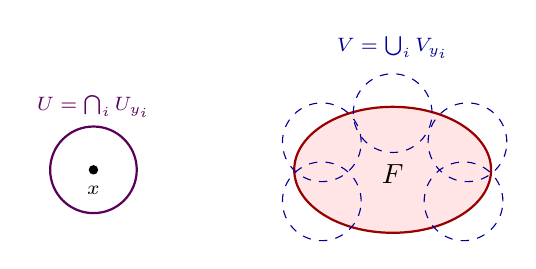
\begin{tikzpicture}[scale=1.0]
\draw[cerrado] (3.0,0) ellipse (1.25 and 0.8);
\node at (3.0,-0.05) {$F$};
\foreach \a/\b in {2.1/0.35,3.0/0.72,3.95/0.35,3.9/-0.4,2.1/-0.4}{
  \draw[blue!60!black,thin,dashed] (\a,\b) circle (0.5);}
\node[pt] at (-0.8,0) {}; \node[below] at (-0.8,-0.08) {\scriptsize $x$};
\draw[violet!70!black,thick] (-0.8,0) circle (0.55);
\node[violet!70!black] at (-0.8,0.8) {\scriptsize $U=\bigcap_i U_{y_i}$};
\node[blue!60!black] at (3.0,1.55) {\scriptsize $V=\bigcup_i V_{y_i}$};
\end{tikzpicture}
\figtit{Figura 22. Separar un punto de un compacto: se separa $x$ de cada $y\in F$, la compacidad deja finitos $V_{y_i}$ (punteados) y del lado de $x$ se intersecan los finitos $U_{y_i}$. Sin compacidad habría que intersecar infinitos abiertos, y eso puede no ser abierto.}
\end{figure}

\begin{corolario}[En un Hausdorff, compacto implica cerrado \fnt{GT 3.3.3, p.\,48; MS Prop.\ 6.9, p.\,82}]\label{cp:compcerr}
En un espacio Hausdorff (en particular, en un métrico), todo compacto es cerrado.
\lgc{X\ \text{es } T_2\ \wedge\ F\ \text{compacto}\ \Rightarrow\ F\ \text{cerrado}.}
\end{corolario}

\begin{proof}
Se ve que $X-F$ es abierto. Si $x\in X-F$, la Prop.~\ref{cp:ptocomp} da $U\ni x$ abierto y $V\supseteq F$ con $U\cap V=\emptyset$; entonces $U\cap F=\emptyset$, o sea $x\in U\subseteq X-F$. Así todo punto de $X-F$ es interior.
\end{proof}

\begin{contraejemplo}[Sin Hausdorff, falla \fnt{MS Contraej.\ 6.2, p.\,82; Ejemplos 6.1(1),(5), p.\,80}]\label{cp:not2}
En la indiscreta sobre un $X$ con dos puntos o más, y en la cofinita sobre un $X$ infinito, \emph{todo} subconjunto es compacto (Ej.~\ref{cp:ejtop}), pero no todo subconjunto es cerrado: en la cofinita, $\N\subseteq\R$ es compacto y no es cerrado. Ninguna de las dos es $T_2$.
\end{contraejemplo}

\begin{corolario}[Compactos de un compacto Hausdorff \fnt{MS Cor.\ 6.10, p.\,82}]\label{cp:compT2}
Si $(X,\tp)$ es compacto y Hausdorff, un subconjunto es compacto si y sólo si es cerrado.
\lgc{X\ \text{compacto}\ \wedge\ X\ \text{es }T_2\ \Rightarrow\ \big(A\ \text{compacto}\iff A\ \text{cerrado}\big).}
Una flecha es la Prop.~\ref{cp:cerrcomp} y la otra el Cor.~\ref{cp:compcerr}.
\end{corolario}

\begin{proposicion}[Separación de dos compactos \fnt{GT 3.3.4 y Nota 3.3.5, pp.\,48--49; MS Prop.\ 6.11, pp.\,82--83}]\label{cp:doscomp}
En un espacio Hausdorff, dos compactos disjuntos $F_1,F_2$ se separan con abiertos disjuntos: existen $U\supseteq F_1$ y $V\supseteq F_2$ abiertos con $U\cap V=\emptyset$.
\lgc{X\ \text{es } T_2\ \wedge\ F_1,F_2\ \text{compactos}\ \wedge\ F_1\cap F_2=\emptyset\\ \Rightarrow\ \exists U,V\in\tp:\ F_1\subseteq U\ \wedge\ F_2\subseteq V\ \wedge\ U\cap V=\emptyset.}
\end{proposicion}

\begin{proof}
Se repite la Prop.~\ref{cp:ptocomp} con $F_1$ en el lugar de $x$. Para cada $x\in F_1$ hay abiertos disjuntos $U_x\ni x$ y $V_x\supseteq F_2$. Los $U_x$ recubren $F_1$: $F_1\subseteq U_{x_1}\cup\dots\cup U_{x_n}=:U$. Sea $V:=V_{x_1}\cap\dots\cap V_{x_n}\supseteq F_2$, abierto. Y $U\cap V\subseteq\bigcup_i(U_{x_i}\cap V_{x_i})=\emptyset$.
\end{proof}

\begin{observacion}[Erratas de \textbf{GT} p.\,48--49]
En la demostración de 3.3.4 \textbf{GT} escribe $V=\bigcup_{i=1}^nV_{x_i}$ (``abierto por ser intersección finita''): debe ser $V=\bigcap_iV_{x_i}$, como arriba; y la conclusión ``$U\cup V=\emptyset$'' es $U\cap V=\emptyset$. En 3.3.1 el último término $(U_{y_n}\cup V_{y_n})$ es $(U_{y_n}\cap V_{y_n})$. La moraleja es la de la figura anterior: \emph{del lado que se cubre se une, del lado de enfrente se interseca}. En un espacio no $T_2$ puede fallar incluso para dos puntos: en $(\R,\tp_{ind})$, $\{1\}$ y $\{2\}$ son compactos disjuntos no separables (\textbf{MS} Contraej.\ 6.3, p.\,83).
\end{observacion}

\begin{teorema}[Heine--Borel en la recta \fnt{GT 3.3.6, p.\,49; MS Ejemplos 6.1(8), p.\,80}]\label{cp:HBR}
En $(\R,\tp_u)$, un subconjunto $A$ es compacto si y sólo si es cerrado y acotado.
\lgc{A\subseteq(\R,\tp_u):\quad A\ \text{compacto}\iff A\ \text{cerrado}\ \wedge\ A\ \text{acotado}.}
\end{teorema}

\begin{proof}
($\Leftarrow$) Cor.~\ref{cp:cerracR}. ($\Rightarrow$) Cerrado por el Cor.~\ref{cp:compcerr} ($\R$ es métrico) y acotado por la Prop.~\ref{cp:acotado}.
\end{proof}

%----------------------------------------------------------------------
\subsection[Compacidad y continuidad]{Compacidad y continuidad \noentra{todavía no dictado en clase}}\label{cp:sub-cont}

\begin{proposicion}[La imagen continua de un compacto es compacta \fnt{GT 3.4.1, p.\,49; MS Prop.\ 6.4 y Cor.\ 6.5, p.\,81}]\label{cp:imcomp}
Sea $f:(X,\tp)\to(Y,\tp')$ continua y $A\subseteq X$ compacto. Entonces $f(A)$ es compacto. En particular, si $X$ es compacto y $f$ es sobreyectiva, $Y$ es compacto, y la compacidad es una propiedad topológica.
\lgc{f\ \text{continua}\ \wedge\ A\ \text{compacto}\ \Rightarrow\ f(A)\ \text{compacto};\\ X\cong Y\Rightarrow\big(X\ \text{compacto}\iff Y\ \text{compacto}\big).}
\end{proposicion}

\begin{proof}
Sea $f(A)\subseteq\bigcup_\alpha G_\alpha$ con $G_\alpha\in\tp'$. Entonces $A\subseteq f^{-1}(f(A))\subseteq\bigcup_\alpha f^{-1}(G_\alpha)$, y cada $f^{-1}(G_\alpha)$ es abierto por continuidad. Por compacidad $A\subseteq f^{-1}(G_{\alpha_1})\cup\dots\cup f^{-1}(G_{\alpha_n})=f^{-1}(G_{\alpha_1}\cup\dots\cup G_{\alpha_n})$, y aplicando $f$ (que cumple $f(f^{-1}(B))\subseteq B$): $f(A)\subseteq G_{\alpha_1}\cup\dots\cup G_{\alpha_n}$.
\end{proof}

\begin{corolario}[Menos abiertos, más compacto \fnt{MS Obs.\ 6.1(3), p.\,80}]
Si $A$ es compacto en $(X,\tp_1)$ y $\tp_2\subseteq\tp_1$, entonces $A$ es compacto en $(X,\tp_2)$: es la imagen de $A$ por $1_X:(X,\tp_1)\to(X,\tp_2)$, continua por la Prop.~\ref{pr:idcont}. (Con menos abiertos hay menos recubrimientos que achicar.)
\lgc{A\ \text{compacto en } (X,\tp_1)\ \wedge\ \tp_2\subseteq\tp_1\Rightarrow A\ \text{compacto en } (X,\tp_2).}
\end{corolario}

\begin{teorema}[Weierstrass \fnt{GT 3.4.2, p.\,49}]\label{cp:weier}
Sea $f:(X,\tp)\to(\R,\tp_u)$ continua y $A\subseteq X$ compacto y no vacío. Entonces $f$ alcanza en $A$ su máximo y su mínimo.
\lgc{f:X\to\R\ \text{continua}\ \wedge\ A\ne\emptyset\ \text{compacto}\ \Rightarrow\ \exists a_1,a_2\in A\ \forall a\in A:\ f(a_1)\le f(a)\le f(a_2).}
\end{teorema}

\begin{proof}
$f(A)$ es compacto en $\R$ (Prop.~\ref{cp:imcomp}), luego cerrado y acotado (Teo.~\ref{cp:HBR}). Como es no vacío y acotado, tiene supremo $s$; el supremo es adherente ($(s-\varepsilon,s]$ corta a $f(A)$ para todo $\varepsilon>0$, \textbf{GT} Ej.\ 2.3.7), y como $f(A)$ es cerrado, $s\in\cl{f(A)}=f(A)$: $s=f(a_2)$. Igual con el ínfimo.
\end{proof}

\begin{observacion}[Errata de \textbf{GT} 3.4.2]
\textbf{GT} no pide $A\ne\emptyset$, y hace falta: el vacío es compacto y $f(\emptyset)=\emptyset$ no tiene máximo. Además, lo que se alcanza son el máximo y el mínimo \emph{de $f$ sobre $A$} (``la imagen alcanza su máximo'' en el texto).
\end{observacion}

\begin{proposicion}[De compacto a Hausdorff, toda continua es cerrada \fnt{GT 3.4.3 y Nota 3.4.4, pp.\,49--50; MS Prop.\ 6.12, p.\,83}]\label{cp:cerrada}
Sea $f:(X,\tp)\to(Y,\tp')$ continua, con $X$ compacto e $Y$ Hausdorff. Entonces $f$ es cerrada: lleva cerrados de $X$ en cerrados de $Y$.
\lgc{f\ \text{continua}\ \wedge\ X\ \text{compacto}\ \wedge\ Y\ \text{es }T_2\ \Rightarrow\ \forall F\ \text{cerrado de } X:\ f(F)\ \text{cerrado de } Y.}
\end{proposicion}

\begin{proof}
Es la cadena de las tres proposiciones anteriores: $F$ cerrado en el compacto $X$ $\Rightarrow$ $F$ compacto (Prop.~\ref{cp:cerrcomp}) $\Rightarrow$ $f(F)$ compacto (Prop.~\ref{cp:imcomp}) $\Rightarrow$ $f(F)$ cerrado en el Hausdorff $Y$ (Cor.~\ref{cp:compcerr}).
\end{proof}

\begin{corolario}[Biyectiva y continua de compacto a Hausdorff es homeomorfismo \fnt{GT 3.4.5, p.\,50; MS Cor.\ 6.13, p.\,83}]\label{cp:homeo}
Si $f:(X,\tp)\to(Y,\tp')$ es continua y biyectiva, $X$ es compacto e $Y$ es Hausdorff, entonces $f$ es un homeomorfismo.
\lgc{f\ \text{continua}\ \wedge\ f\ \text{biyectiva}\ \wedge\ X\ \text{compacto}\ \wedge\ Y\ \text{es }T_2\ \Rightarrow\ f\ \text{homeomorfismo}.}
\end{corolario}

\begin{proof}
$f$ es cerrada (Prop.~\ref{cp:cerrada}); una biyección continua y cerrada es homeomorfismo (caracterizaciones de \S\ref{sec:homeo}). Directamente: para $F$ cerrado de $X$, $(f^{-1})^{-1}(F)=f(F)$ es cerrado, así que $f^{-1}$ es continua.
\end{proof}

\begin{observacion}
\textbf{GT} pide que $X$ e $Y$ sean los dos compactos y Hausdorff; como dice su Nota 3.4.4, sólo se usa que $X$ sea compacto e $Y$ Hausdorff. Las dos hipótesis son necesarias:
\begin{lista}
\item sin compacidad del dominio: $t\mapsto(\cos t,\sin t)$ de $[0,2\pi)$ en $S^1$ es biyectiva y continua y no es homeomorfismo (\S\ref{sec:homeo}; \textbf{MS} Contraej.\ 6.4, p.\,83). $[0,2\pi)$ no es compacto: justamente, el ``agujero'' en $2\pi$ es lo que rompe la continuidad de la inversa;
\item sin Hausdorff en el codominio: $1_X:(X,\tp_{dis})\to(X,\tp_{ind})$ con $X$ finito de dos puntos o más es biyectiva y continua, el dominio es compacto (finito) y no es homeomorfismo.
\end{lista}
\end{observacion}

\begin{ejemplo}[La circunferencia es compacta \fnt{GT Ej.\ 3.4.6, p.\,50}]
$S^1=f([0,2\pi])$ con $f(t)=(\cos t,\sin t)$, continua porque sus coordenadas lo son (Prop.~\ref{pr:coord}), y $[0,2\pi]$ es compacto (Teo.~\ref{cp:ab}). Luego $S^1$ es compacto en $\R^2$.
\end{ejemplo}

\begin{ejemplo}[Intersección de compactos \fnt{GT Ej.\ 3.4.7, p.\,50; MS Obs.\ 6.1(4), p.\,80, y \S6.5, Problema 4(ii), p.\,84}]\label{cp:intercomp}
En un espacio Hausdorff (en particular, métrico), la intersección de una familia no vacía de compactos $\{A_\alpha\}$ es compacta: cada $A_\alpha$ es cerrado (Cor.~\ref{cp:compcerr}), así que $\bigcap_\alpha A_\alpha$ es cerrado y está contenido en un $A_{\alpha_0}$ compacto (Prop.~\ref{cp:cerrcomp}).
\lgc{X\ \text{es }T_2\ \wedge\ \forall\alpha\ A_\alpha\ \text{compacto}\ \wedge\ \Lambda\ne\emptyset\ \Rightarrow\ \textstyle\bigcap_{\alpha\in\Lambda}A_\alpha\ \text{compacto}.}
Sin Hausdorff puede fallar. Sea $X=\N\cup\{a,b\}$ (con $a,b\notin\N$ distintos) y $\tp=\mathcal P(\N)\cup\{G\subseteq X:\ G\cap\{a,b\}\ne\emptyset\ \wedge\ \N-G\ \text{finito}\}$ (se verifica que es topología). $K_1=\N\cup\{a\}$ y $K_2=\N\cup\{b\}$ son compactos: el abierto del recubrimiento que contiene a $a$ (resp.\ $b$) deja afuera finitos naturales. Pero $K_1\cap K_2=\N$ es un subespacio discreto infinito, no compacto. Y $K_1$ es compacto y no es cerrado ($\{b\}$ no es abierto).
\end{ejemplo}

\begin{ejemplo}[Encajados de Cantor \fnt{GT Ej.\ 3.4.8, pp.\,50--51}]\label{cp:cantor}
Sea $F_1\supseteq F_2\supseteq\cdots$ una sucesión de cerrados no vacíos con $F_1$ compacto. Entonces $\bigcap_{n}F_n\ne\emptyset$. En efecto, la familia tiene la PIF (una intersección finita $F_{n_1}\cap\dots\cap F_{n_k}$ es el de índice mayor, no vacío), y los $F_n=F_n\cap F_1$ son cerrados del espacio compacto $F_1$ (Teo.~\ref{cp:pif}). Es lo que pasa con el conjunto de Cantor (\textbf{GT} Ej.\ 2.6.6(c)). \textbf{GT} pide además que $X$ sea Hausdorff, pero no se usa. Con $F_1$ no compacto falla: $F_n=[n,\infty)$ en $\R$.
\lgc{F_1\supseteq F_2\supseteq\cdots\ \text{cerrados}\ \wedge\ F_n\ne\emptyset\ \wedge\ F_1\ \text{compacto}\ \Rightarrow\ \textstyle\bigcap_{n\ge1}F_n\ne\emptyset.}
\end{ejemplo}

%----------------------------------------------------------------------
\subsection[Compacidad en productos]{Compacidad en productos: lema del tubo y Tychonoff finito \noentra{todavía no dictado en clase}}\label{cp:sub-prod}

\noindent \textbf{GT} \S3.5 prueba que el producto de compactos es compacto sólo para métricos con $\delta^{\max}_n$ (3.5.1) y en la Nota 3.5.5 dice que la demostración ``similar'' vale para la topología producto. Acá se hace directamente con la topología producto de \S\ref{sec:prod}, con el argumento de los tubos (Prop.~\ref{pr:tubos}); la versión métrica sale de que las métricas producto inducen la topología producto (Obs.~\ref{ob:prodfin}).

\begin{lema}[Lema del tubo \fnt{versión topológica de GT 3.5.1 y Nota 3.5.5, pp.\,51--53; MS Teo.\ 6.6, p.\,81}]\label{cp:tubo}
Sean $X$ e $Y$ espacios topológicos con $Y$ compacto, $x_0\in X$, y $W$ un abierto de $X\times Y$ que contiene a toda la fibra $\{x_0\}\times Y$. Entonces existe un abierto $U\ni x_0$ de $X$ tal que el tubo entero $U\times Y$ queda dentro de $W$.
\lgc{Y\ \text{compacto}\ \wedge\ W\in\tp_{X\times Y}\ \wedge\ \{x_0\}\times Y\subseteq W\ \Rightarrow\ \exists U\in\tp_X:\ x_0\in U\ \wedge\ U\times Y\subseteq W.}
\end{lema}

\begin{proof}
Para cada $y\in Y$, $(x_0,y)\in W$ y $W$ es abierto del producto, así que hay un rectángulo básico con $(x_0,y)\in U_y\times V_y\subseteq W$ ($U_y\in\tp_X$, $V_y\in\tp_Y$). Los $\{V_y\}_{y\in Y}$ recubren $Y$; como $Y$ es compacto, $Y=V_{y_1}\cup\dots\cup V_{y_n}$. Sea $U:=U_{y_1}\cap\dots\cap U_{y_n}$: es abierto (intersección \emph{finita}) y contiene a $x_0$. Si $(x,y)\in U\times Y$, hay $i$ con $y\in V_{y_i}$, y $x\in U\subseteq U_{y_i}$, así que $(x,y)\in U_{y_i}\times V_{y_i}\subseteq W$. (Si $Y=\emptyset$, sirve $U=X$.)
\end{proof}

\begin{figure}[ht]
\centering
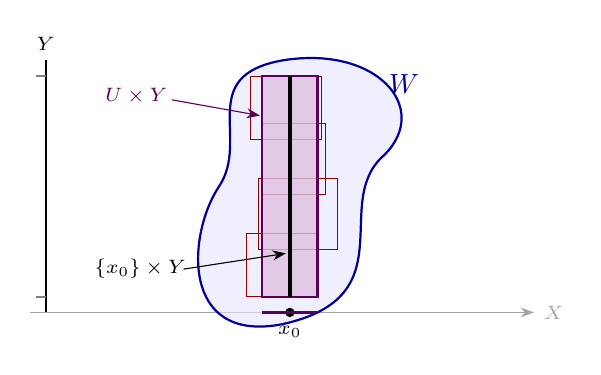
\begin{tikzpicture}[scale=1.0]
\draw[ejes] (-0.2,0)--(6.2,0) node[right]{\scriptsize $X$};
\draw[thick] (0,0)--(0,3.2) node[above]{\scriptsize $Y$};
\draw[thick,gray] (0,0.2)--(-0.12,0.2) (0,3.0)--(-0.12,3.0);
% W
\draw[abierto,fill opacity=0.6] (3.0,-0.15) .. controls (4.6,0.2) and (3.6,1.4) .. (4.3,2.0)
  .. controls (4.9,2.6) and (4.2,3.4) .. (3.0,3.2)
  .. controls (1.9,3.0) and (2.6,2.2) .. (2.2,1.6)
  .. controls (1.8,1.0) and (1.7,-0.4) .. (3.0,-0.15);
\node[blue!60!black] at (4.55,2.9) {$W$};
% rectangulos
\foreach \yb/\yt/\xl/\xr in {0.2/1.0/2.55/3.45, 0.8/1.7/2.7/3.7, 1.5/2.4/2.75/3.55, 2.2/3.0/2.6/3.5}{
  \draw[red!60!black,thin] (\xl,\yb) rectangle (\xr,\yt);}
% tubo
\fill[violet!25,opacity=0.8] (2.75,0.2) rectangle (3.45,3.0);
\draw[violet!70!black,thick] (2.75,0.2) rectangle (3.45,3.0);
% fibra
\draw[very thick] (3.1,0.2)--(3.1,3.0);
\node[pt] at (3.1,0) {}; \node[below] at (3.1,-0.05) {\scriptsize $x_0$};
\draw[violet!70!black,very thick] (2.75,0)--(3.45,0);
\node[violet!70!black] at (1.15,2.75) {\scriptsize $U\times Y$};
\draw[->,>=Stealth,thin,violet!70!black] (1.6,2.7)--(2.72,2.5);
\node at (1.2,0.55) {\scriptsize $\{x_0\}\times Y$};
\draw[->,>=Stealth,thin] (1.75,0.55)--(3.05,0.75);
\end{tikzpicture}
\figtit{Figura 23. El lema del tubo. La fibra compacta $\{x_0\}\times Y$ (negro) se cubre con finitos rectángulos $U_{y_i}\times V_{y_i}\subseteq W$ (rojo); la intersección de sus bases, $U$, da un tubo $U\times Y$ (violeta) todavía dentro de $W$. Es el tubo de la Figura 12, ahora ``engordando'' una fibra.}
\end{figure}

\begin{observacion}[Sin compacidad no hay tubo]
En $\R\times\R$ el abierto $W=\{(x,y): |xy|<1\}$ contiene a la fibra $\{0\}\times\R$, pero ningún tubo $(-\varepsilon,\varepsilon)\times\R$: el punto $(\tfrac\varepsilon2,\tfrac4\varepsilon)$ está en el tubo y no en $W$. El borde de $W$ son las hipérbolas $xy=\pm1$, que se pegan al eje vertical sin tocarlo: es el mismo fenómeno que hace que la proyección de la hipérbola no sea cerrada (\S\ref{sec:prod}). La fibra $\R$ no es compacta, y la intersección de los infinitos $U_y$ se achica a $\{0\}$.
\end{observacion}

\begin{teorema}[Tychonoff, caso finito \fnt{MS Teo.\ 6.6, p.\,81; GT 3.5.1 y Nota 3.5.5, pp.\,51--53}]\label{cp:tych}
Sean $X$ e $Y$ espacios topológicos. Si $X$ e $Y$ son compactos, $X\times Y$ (con la topología producto) es compacto. Recíprocamente, si $X\times Y\ne\emptyset$ es compacto, $X$ e $Y$ lo son. Por inducción, lo mismo vale para $X_1\times\dots\times X_n$.
\lgc{X,Y\ \text{compactos}\Rightarrow X\times Y\ \text{compacto};\qquad X\times Y\ne\emptyset\ \text{compacto}\Rightarrow X,Y\ \text{compactos}.}
\end{teorema}

\begin{proof}
Sea $\{W_\alpha\}$ un recubrimiento abierto de $X\times Y$. Se fija $x\in X$. La fibra $\{x\}\times Y$ es compacta: es la imagen de $Y$ por $y\mapsto(x,y)$, continua (Cor.~\ref{co:fxg}), y se aplica la Prop.~\ref{cp:imcomp}. Entonces la cubren finitos $W_\alpha$; su unión $W_x$ es un abierto que contiene a $\{x\}\times Y$. Por el lema del tubo hay $U_x\ni x$ abierto con $U_x\times Y\subseteq W_x$.

Los $\{U_x\}_{x\in X}$ recubren $X$, compacto: $X=U_{x_1}\cup\dots\cup U_{x_m}$. Luego
\[
X\times Y=\textstyle\bigcup_{j=1}^m U_{x_j}\times Y\subseteq\bigcup_{j=1}^m W_{x_j},
\]
y cada $W_{x_j}$ es unión de finitos $W_\alpha$: en total, finitos $W_\alpha$ cubren $X\times Y$.
Recíproca: $\pi_X$ es continua y, si $X\times Y\ne\emptyset$, sobreyectiva; así $X=\pi_X(X\times Y)$ es compacto (Prop.~\ref{cp:imcomp}). Igual $Y$.
\end{proof}

\begin{intuicion}
Es un ``doble paso a finitos'': primero en la dirección de $Y$ (cada fibra vertical se cubre con finitos, y el lema del tubo engorda esa fibra a un tubo), después en la dirección de $X$ (finitos tubos cubren todo). La compacidad de $Y$ es la que permite intersecar los $U_{y_i}$ sin perder la apertura.
\end{intuicion}

\begin{observacion}[Subconjuntos compactos de un producto]
Si $A\subseteq X$ y $B\subseteq Y$ son compactos, $A\times B$ es compacto en $X\times Y$ (que es el enunciado de \textbf{GT} 3.5.1). Por el Lema~\ref{cp:absoluta} alcanza con ver que la topología de subespacio de $A\times B$ en $X\times Y$ es la topología producto de $(A,\tp_A)\times(B,\tp_B)$; y eso es porque las dos tienen la misma base: $(U\times V)\cap(A\times B)=(U\cap A)\times(V\cap B)$.
\end{observacion}

\begin{proposicion}[Proyección a lo largo de un factor compacto \fnt{MS \S6.5, Problema 7, p.\,84}]\label{cp:proycerr}
Si $X$ es compacto, la proyección $\pi_Y:X\times Y\to Y$ es cerrada. (Compárese con la hipérbola de \S\ref{sec:prod}: allí el factor que se ``aplasta'' es $\R$, no compacto.)
\lgc{X\ \text{compacto}\ \Rightarrow\ \forall F\ \text{cerrado de } X\times Y:\ \pi_Y(F)\ \text{cerrado de } Y.}
\end{proposicion}

\begin{proof}
Sea $F$ cerrado y $y_0\notin\pi_Y(F)$. Entonces la fibra $X\times\{y_0\}$ no corta a $F$: está en el abierto $W=(X\times Y)-F$. Por el lema del tubo (con los papeles de los factores cambiados) hay $V\ni y_0$ abierto con $X\times V\subseteq W$, es decir, $X\times V$ no corta a $F$, o sea $V\cap\pi_Y(F)=\emptyset$. Así $Y-\pi_Y(F)$ es abierto.
\end{proof}

\begin{corolario}[Cajas compactas \fnt{GT 3.5.2, p.\,52}]\label{cp:cajas}
En $(\R^n,\tp_u)$, todo producto de intervalos $[a_1,b_1]\times\dots\times[a_n,b_n]$ es compacto.
\lgc{[a_1,b_1]\times\dots\times[a_n,b_n]\ \text{compacto en } (\R^n,\tp_u).}
\end{corolario}

\begin{proof}
Cada $[a_i,b_i]$ es compacto (Teo.~\ref{cp:ab}), el producto es compacto (Teo.~\ref{cp:tych}) y la topología producto de $n$ copias de $\R$ es la usual de $\R^n$ (Obs.~\ref{ob:prodfin}); con $d_e$, $d_{\max}$ o $d_{\text{taxi}}$ da lo mismo (Prop.~\ref{pr:equiv}).
\end{proof}

\begin{teorema}[Heine--Borel en $\R^n$ \fnt{GT 3.5.3, pp.\,52--53; MS \S6.5, Problema 2, p.\,83}]\label{cp:HB}
En $(\R^n,\tp_u)$, un subconjunto $A$ es compacto si y sólo si es cerrado y acotado.
\lgc{A\subseteq(\R^n,\tp_u):\quad A\ \text{compacto}\iff A\ \text{cerrado}\ \wedge\ A\ \text{acotado}.}
\end{teorema}

\begin{proof}
($\Rightarrow$) $\R^n$ es métrico, luego Hausdorff: $A$ es cerrado (Cor.~\ref{cp:compcerr}) y acotado (Prop.~\ref{cp:acotado}). ($\Leftarrow$) Si $A$ es acotado está en una bola euclídea $\Bola{0}{r}$, y por lo tanto en una caja $J=[-r,r]^n$ (la bola de $d_{\max}$ de radio $r$ contiene a la de $d_e$). $J$ es compacto (Cor.~\ref{cp:cajas}) y $A=A\cap J$ es compacto por ser cerrado dentro de un compacto (Prop.~\ref{cp:cerrcomp}).
\end{proof}

\begin{observacion}[Errata y alcance \fnt{GT 3.5.3 y Nota 3.5.4, pp.\,52--53}]
El enunciado de \textbf{GT} dice ``$A\subseteq\R$'': es $A\subseteq\R^n$. La implicación ($\Rightarrow$) vale en todo métrico (Nota 3.5.4); ($\Leftarrow$) es propia de $\R^n$ y falla en general:
\begin{lista}
\item en $(\N,d_D)$ el espacio entero es cerrado y acotado ($\delta=1$), y no es compacto (discreto infinito, Ej.~\ref{cp:ejtop});
\item en $(\Q,d_e)$, $[0,2]\cap\Q$ es cerrado (en $\Q$) y acotado, y no es compacto (Ej.~\ref{cp:ejlc});
\item en el espacio de funciones continuas, la bola cerrada unidad (Ej.~\ref{cp:bolafun}).
\end{lista}
\end{observacion}

%----------------------------------------------------------------------
\subsection[Compacidad en espacios métricos]{Compacidad en espacios métricos \noentra{todavía no dictado en clase}}\label{cp:sub-met}

\begin{definicion}[Subsucesión, compacidad secuencial \fnt{GT 3.6.2--3.6.3, p.\,54; MS Defs.\ 6.4--6.5, p.\,82}]
Una \emph{subsucesión} de $\{x_n\}_{n\ge1}$ es una sucesión $\{x_{n_k}\}_{k\ge1}$ con $n_1<n_2<\cdots$ índices estrictamente crecientes. $(X,\tp)$ es \emph{secuencialmente compacto} si toda sucesión en $X$ tiene una subsucesión convergente (en $X$). \textbf{GT} llama a esto \emph{propiedad de Bolzano--Weierstrass}; en \textbf{MS} ese nombre se reserva para ``todo subconjunto infinito tiene un punto de acumulación''. En métricos las tres cosas son equivalentes a la compacidad (\textbf{MS} Prop.\ 6.7); en topológicos generales no hay relación entre compacidad y compacidad secuencial.
\lgc{X\ \text{secuencialmente compacto}\iff \forall\{x_n\}_{n\ge1}\subseteq X\ \exists n_1<n_2<\cdots\ \exists x_0\in X:\ x_{n_k}\xrightarrow[k\to\infty]{}x_0.}
\end{definicion}

\begin{proposicion}[Compacto métrico $\Rightarrow$ secuencialmente compacto \fnt{GT 3.6.1--3.6.2, pp.\,53--54}]\label{cp:compsec}
Sea $(X,d)$ métrico compacto. Entonces toda sucesión en $X$ tiene una subsucesión convergente.
\lgc{(X,d)\ \text{compacto}\ \Rightarrow\ \forall\{x_n\}\subseteq X\ \exists\{x_{n_k}\}_{k\ge1}\ \exists x_0\in X:\ x_{n_k}\to x_0.}
\end{proposicion}

\begin{proof}
(Reorganización de la de \textbf{GT}.) Primero: si para cierto $x_0$ \emph{toda} bola $\Bola{x_0}{r}$ contiene $x_n$ para infinitos índices $n$, entonces una subsucesión converge a $x_0$: se elige $n_1$ con $x_{n_1}\in\Bola{x_0}{1}$, $n_2>n_1$ con $x_{n_2}\in\Bola{x_0}{1/2}$, \dots, $n_k>n_{k-1}$ con $x_{n_k}\in\Bola{x_0}{1/k}$ (siempre se puede, porque hay infinitos índices disponibles), y $d(x_{n_k},x_0)<1/k\to0$.
Ahora, por el absurdo: si ninguna subsucesión converge, cada $x\in X$ tiene una bola $\Bola{x}{r_x}$ que contiene $x_n$ sólo para \emph{finitos} índices $n$. Esas bolas recubren $X$; por compacidad, finitas lo hacen. Entonces todos los índices $n\in\N$ están entre los finitos índices asociados a finitas bolas: absurdo, porque $\N$ es infinito.
\end{proof}

\begin{definicion}[Totalmente acotado \fnt{nombre de curso; es la propiedad de GT 3.6.4, p.\,54}]
$(X,d)$ es \emph{totalmente acotado} si para cada $\varepsilon>0$ se puede cubrir con una cantidad finita de bolas de radio $\varepsilon$. (\textbf{GT} enuncia la propiedad sin darle nombre.) Totalmente acotado implica acotado; la recíproca es falsa: $(\N,d_D)$ es acotado y no se cubre con finitas bolas de radio $\tfrac12$ (que son unitarios).
\lgc{(X,d)\ \text{totalmente acotado}\iff \forall\varepsilon>0\ \exists x_1,\dots,x_n\in X:\ X=\Bola{x_1}{\varepsilon}\cup\dots\cup\Bola{x_n}{\varepsilon}.}
\end{definicion}

\begin{proposicion}[Secuencialmente compacto $\Rightarrow$ totalmente acotado \fnt{GT 3.6.4, pp.\,54--55}]\label{cp:totac}
Si $(X,d)$ es métrico y secuencialmente compacto, entonces es totalmente acotado.
\lgc{(X,d)\ \text{sec. compacto}\ \Rightarrow\ \forall\varepsilon>0\ \exists x_1,\dots,x_n:\ X=\textstyle\bigcup_{i=1}^n\Bola{x_i}{\varepsilon}.}
\end{proposicion}

\begin{proof}
Si para cierto $\varepsilon_0$ ninguna cantidad finita de bolas de radio $\varepsilon_0$ cubre $X$, se construye por recurrencia una sucesión $\varepsilon_0$-separada: $x_1$ cualquiera, y $x_{n+1}\notin\Bola{x_1}{\varepsilon_0}\cup\dots\cup\Bola{x_n}{\varepsilon_0}$ (existe, porque esas $n$ bolas no cubren). Así $d(x_n,x_m)\ge\varepsilon_0$ si $n\ne m$. Ninguna subsucesión converge: si $x_{n_k}\to x_0$, para $k,s$ grandes $d(x_{n_k},x_{n_s})\le d(x_{n_k},x_0)+d(x_0,x_{n_s})<\tfrac{\varepsilon_0}2+\tfrac{\varepsilon_0}2$. Absurdo.
\end{proof}

\begin{lema}[Lema de Lebesgue \fnt{GT 3.6.5 y Nota 3.6.6, pp.\,55--56}]\label{cp:lebesgue}
Sea $(X,d)$ métrico secuencialmente compacto y $\{U_\alpha\}_{\alpha\in\Lambda}$ un recubrimiento de $X$ por abiertos. Entonces existe $\varepsilon>0$ (un \emph{número de Lebesgue} del recubrimiento) tal que toda bola de radio $\varepsilon$ está contenida en algún $U_\alpha$. En consecuencia, todo $A\subseteq X$ no vacío con $\delta(A)<\varepsilon$ está contenido en algún $U_\alpha$.
\lgc{\exists\varepsilon>0\ \forall x\in X\ \exists\alpha\in\Lambda:\ \Bola{x}{\varepsilon}\subseteq U_\alpha;\qquad \emptyset\ne A\subseteq X\ \wedge\ \delta(A)<\varepsilon\ \Rightarrow\ \exists\alpha:\ A\subseteq U_\alpha.}
\end{lema}

\begin{proof}
Por el absurdo: si ningún $\varepsilon$ sirve, para $\varepsilon=\tfrac1n$ hay $x_n$ con $\Bola{x_n}{\tfrac1n}$ no contenida en ningún $U_\alpha$. Una subsucesión converge, $x_{n_k}\to x_0$, y $x_0$ está en algún $U_{\alpha_0}$ abierto: $\Bola{x_0}{\delta}\subseteq U_{\alpha_0}$. Se toma $k$ con $d(x_{n_k},x_0)<\tfrac\delta2$ y $\tfrac1{n_k}<\tfrac\delta2$. Si $y\in\Bola{x_{n_k}}{\tfrac1{n_k}}$, $d(y,x_0)<\tfrac1{n_k}+\tfrac\delta2<\delta$; o sea $\Bola{x_{n_k}}{\tfrac1{n_k}}\subseteq\Bola{x_0}{\delta}\subseteq U_{\alpha_0}$, contra la elección de $x_{n_k}$.
Para la consecuencia: si $a\in A$ y $\delta(A)<\varepsilon$, entonces $A\subseteq\Bola{a}{\varepsilon}$, que está en algún $U_\alpha$.
\end{proof}

\begin{intuicion}
El número de Lebesgue dice que un recubrimiento abierto de un compacto métrico tiene un ``grosor mínimo'': todo conjunto suficientemente chico cae \emph{entero} en uno de los abiertos. En $(0,1)$ con el recubrimiento $\{(\tfrac1k,1)\}$ no hay grosor mínimo: cerca de $0$ los abiertos que cubren son cada vez más finos en ese extremo. Es el mismo fenómeno que el lema del tubo, en versión métrica.
\end{intuicion}

\begin{observacion}[Errata de \textbf{GT} 3.6.5]
El enunciado dice ``cualquier recubrimiento'': tiene que ser \emph{por abiertos} (con $\{\{x\}\}_{x\in X}$ falla). En la demostración aparece $G_\alpha$ en lugar de $U_\alpha$. En 3.6.4, ``$x_2\notin B_d(x,\varepsilon_0)$'' es $x_2\notin B_d(x_1,\varepsilon_0)$.
\end{observacion}

\begin{teorema}[Bolzano--Weierstrass: en métricos, compacto $\iff$ secuencialmente compacto \fnt{GT 3.6.3, p.\,54, demostración en p.\,56; MS Prop.\ 6.7, p.\,82}]\label{cp:BW}
Un espacio métrico $(X,d)$ es compacto si y sólo si toda sucesión en $X$ tiene una subsucesión convergente.
\lgc{(X,d)\ \text{compacto}\iff \forall\{x_n\}\subseteq X\ \exists\{x_{n_k}\}\ \exists x_0\in X:\ x_{n_k}\to x_0.}
\end{teorema}

\begin{proof}
($\Rightarrow$) Prop.~\ref{cp:compsec}. ($\Leftarrow$) Sea $\{U_\alpha\}$ un recubrimiento abierto y $\varepsilon$ un número de Lebesgue (Lema~\ref{cp:lebesgue}). Por la Prop.~\ref{cp:totac}, $X=\Bola{x_1}{\varepsilon}\cup\dots\cup\Bola{x_n}{\varepsilon}$, y cada $\Bola{x_i}{\varepsilon}$ está en algún $U_{\alpha_i}$. Luego $X=U_{\alpha_1}\cup\dots\cup U_{\alpha_n}$.
\end{proof}

\begin{observacion}
Para un subconjunto $A$ de un métrico: $A$ es compacto sii toda sucesión de puntos de $A$ tiene una subsucesión que converge \emph{a un punto de $A$} (se aplica el teorema al subespacio $(A,d|_A)$, Lema~\ref{cp:absoluta} y Prop.~\ref{pr:subesp}(v)). Es la forma más cómoda de probar que algo \emph{no} es compacto en un métrico: exhibir una sucesión sin subsucesiones convergentes en $A$.
\end{observacion}

\begin{teorema}[Heine: continua en compacto es uniformemente continua \fnt{GT 3.6.7--3.6.8, pp.\,56--57}]\label{cp:heine}
Sea $f:(X,d)\to(Y,\rho)$ continua, con $(X,d)$ compacto. Entonces $f$ es uniformemente continua (definición en \S\ref{sec:unif}, que es la \textbf{GT} 3.6.7).
\lgc{(X,d)\ \text{compacto}\ \wedge\ f\ \text{continua}\\ \Rightarrow\ \forall\varepsilon>0\ \exists\mu>0\\ \forall x,x'\in X:\ d(x,x')<\mu\Rightarrow\rho\big(f(x),f(x')\big)<\varepsilon.}
\end{teorema}

\begin{proof}
Dado $\varepsilon>0$, los conjuntos $f^{-1}\big(B_\rho(y,\tfrac\varepsilon2)\big)$, $y\in Y$, son abiertos (continuidad) y recubren $X$. Sea $\mu$ un número de Lebesgue de ese recubrimiento (Lema~\ref{cp:lebesgue}, aplicable por el Teo.~\ref{cp:BW}). Si $d(x,x')<\mu$, entonces $\{x,x'\}\subseteq\Bola{x}{\mu}\subseteq f^{-1}\big(B_\rho(y_0,\tfrac\varepsilon2)\big)$ para algún $y_0$, así que $\rho(f(x),f(x'))\le\rho(f(x),y_0)+\rho(y_0,f(x'))<\varepsilon$.
\end{proof}

\begin{observacion}
La compacidad es necesaria: $x\mapsto x^2$ en $\R$ y $x\mapsto\tfrac1x$ en $(0,1)$ son continuas y no uniformemente continuas (\S\ref{sec:unif}). Nota: la continuidad uniforme sí figura en \textbf{GT}, como Def.\ 3.6.7.
\end{observacion}

\begin{ejemplo}[Cerrado y acotado que no es compacto \fnt{GT Ej.\ 3.6.9, p.\,57}]\label{cp:bolafun}
Sea $X=\{f:[0,1]\to[0,1]\ \text{continua}\}$ con $d_\infty(f,g)=\max_{x\in[0,1]}|f(x)-g(x)|$, $\theta$ la función nula y $0<\varepsilon\le1$. La bola cerrada $A=\Bolac{\theta}{\varepsilon}$ es cerrada y acotada, pero no es compacta. Las ``rampas'' $f_n(x)=\varepsilon\max\{0,1-(n+1)x\}$ están en $A$ (valen $\varepsilon$ en $0$ y $0$ desde $\tfrac1{n+1}$), y $d_\infty(f_n,\theta)=\varepsilon$. Si una subsucesión $f_{n_k}$ convergiera a $f_0\in A$, convergería punto a punto; para cada $x>0$ es $f_{n_k}(x)=0$ a partir de cierto $k$, así que $f_0(x)=0$, y por continuidad $f_0(0)=0$: $f_0=\theta$. Pero $d_\infty(f_{n_k},\theta)=\varepsilon\not\to0$. Por el Teo.~\ref{cp:BW}, $A$ no es compacto.
\end{ejemplo}

\begin{figure}[ht]
\centering
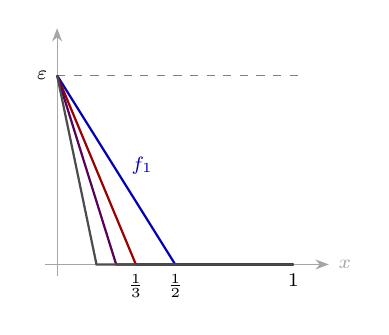
\begin{tikzpicture}[scale=3.0]
\draw[ejes] (-0.05,0)--(1.15,0) node[right]{\scriptsize $x$};
\draw[ejes] (0,-0.05)--(0,1.0);
\draw[gray,dashed] (0,0.8)--(1.05,0.8);
\node[left] at (0,0.8) {\scriptsize $\varepsilon$};
\foreach \n/\c in {1/blue!70!black,2/red!60!black,3/violet!70!black,5/gray!60!black}{
  \draw[thick,\c] (0,0.8)--({1/(\n+1)},0)--(1,0);}
\node[below] at (0.5,0) {\scriptsize $\tfrac12$};
\node[below] at (0.333,0) {\scriptsize $\tfrac13$};
\node[below] at (1,0) {\scriptsize $1$};
\node[blue!70!black] at (0.36,0.42) {\scriptsize $f_1$};
\end{tikzpicture}
\figtit{Figura 24. Las rampas de GT Ej.\ 3.6.9: todas a distancia $\varepsilon$ de $\theta$, con soporte cada vez más angosto. Punto a punto tienden a una función discontinua ($\varepsilon$ en $0$, $0$ en el resto), así que ninguna subsucesión converge uniformemente.}
\end{figure}

\begin{observacion}[Errata menor de \textbf{GT} 3.6.9]
\textbf{GT} toma ``$\varepsilon$ arbitrario''; como las funciones van a $[0,1]$, las rampas de altura $\varepsilon$ exigen $\varepsilon\le1$ (para $\varepsilon>1$ la bola es todo $X$ y sirven las mismas rampas de altura $1$).
\end{observacion}

%----------------------------------------------------------------------
\subsection[Compacidad y completitud]{Compacidad y completitud \noentra{todavía no dictado en clase}}\label{cp:sub-compl}

\begin{definicion}[Sucesión de Cauchy, espacio completo \fnt{GT 3.7.1 y 3.7.4, p.\,58}]
En $(X,d)$, una sucesión $\{x_n\}$ es \emph{de Cauchy} si sus términos se acercan entre sí: para cada $\varepsilon>0$ hay $n_0$ con $d(x_n,x_{n'})<\varepsilon$ para todos $n,n'\ge n_0$. $(X,d)$ es \emph{completo} si toda sucesión de Cauchy converge en $X$.
\lgc{\{x_n\}\ \text{de Cauchy}\iff\forall\varepsilon>0\ \exists n_0\ \forall n,n'\ge n_0:\ d(x_n,x_{n'})<\varepsilon;\\
(X,d)\ \text{completo}\iff \forall\{x_n\}\ \text{de Cauchy}\ \exists x_0\in X:\ x_n\to x_0.}
\end{definicion}

\begin{proposicion}[\fnt{GT 3.7.2--3.7.3, p.\,58}]\label{cp:cauchy}
Toda sucesión de Cauchy está acotada, y toda sucesión convergente es de Cauchy.
\lgc{\{x_n\}\ \text{de Cauchy}\Rightarrow \delta(\{x_n: n\ge1\})<\infty;\qquad x_n\to x_0\Rightarrow\{x_n\}\ \text{de Cauchy}.}
\end{proposicion}

\begin{proof}
Con $\varepsilon=1$, a partir de $n_0$ todos están a distancia $<1$ de $x_{n_0}$, y quedan finitos términos antes: todos están en la bola de centro $x_{n_0}$ y radio $r>\max\{1,d(x_{n_0},x_i): i<n_0\}$. Si $x_n\to x_0$: $d(x_n,x_{n'})\le d(x_n,x_0)+d(x_0,x_{n'})<\tfrac\varepsilon2+\tfrac\varepsilon2$ para $n,n'$ grandes.
\end{proof}

\begin{proposicion}[Compacto métrico $\Rightarrow$ completo \fnt{GT 3.7.5, p.\,58}]\label{cp:compcompl}
Todo espacio métrico compacto es completo.
\lgc{(X,d)\ \text{compacto}\ \Rightarrow\ (X,d)\ \text{completo}.}
\end{proposicion}

\begin{proof}
Sea $\{x_n\}$ de Cauchy. Por el Teo.~\ref{cp:BW} tiene una subsucesión $x_{n_k}\to x_0$. Se ve que \emph{toda} la sucesión converge a $x_0$: dado $\varepsilon$, hay $n_0$ con $d(x_n,x_{n'})<\tfrac\varepsilon2$ para $n,n'\ge n_0$ (Cauchy) y $k_0$ con $d(x_{n_k},x_0)<\tfrac\varepsilon2$ para $k\ge k_0$. Para $n\ge n_0$ se elige $k\ge k_0$ con $n_k\ge n_0$, y $d(x_n,x_0)\le d(x_n,x_{n_k})+d(x_{n_k},x_0)<\varepsilon$.
\end{proof}

\begin{corolario}[$\R^n$ es completo \fnt{GT 3.7.6, p.\,58}]\label{cp:Rncompl}
$(\R^n,d_e)$ es completo.
\lgc{\forall\{x_n\}\subseteq\R^n\ \text{de Cauchy}\ \exists x_0\in\R^n:\ x_n\to x_0.}
\end{corolario}

\begin{proof}
Una sucesión de Cauchy está acotada (Prop.~\ref{cp:cauchy}), así que vive en una bola cerrada $K=\Bolac{x_1}{r}$, que es compacta por Heine--Borel (Teo.~\ref{cp:HB}). En el métrico compacto $(K,d_e)$ es de Cauchy, luego converge a un punto de $K$ (Prop.~\ref{cp:compcompl}), y por lo tanto converge en $\R^n$.
\end{proof}

\begin{observacion}
La recíproca de la Prop.~\ref{cp:compcompl} es falsa: $\R$ es completo y no compacto. Y la completitud \emph{no} es una propiedad topológica: $(0,1)\cong\R$ (\textbf{GT} 2.8.17), pero $(0,1)$ no es completo ($x_n=\tfrac1n$ es de Cauchy y no converge en $(0,1)$). La compacidad sí lo es (Prop.~\ref{cp:imcomp}).
\end{observacion}

%----------------------------------------------------------------------
\subsection[Compacidad local]{Compacidad local \noentra{todavía no dictado en clase}}\label{cp:sub-loc}

\begin{definicion}[Localmente compacto \fnt{GT 3.8.1, p.\,59}]
$(X,\tp)$ es \emph{localmente compacto} si cada punto tiene entornos compactos arbitrariamente chicos: para todo $x\in X$ y todo entorno $N$ de $x$ existe un entorno $N'$ de $x$ compacto con $N'\subseteq N$.
\lgc{X\ \text{localmente compacto}\iff \forall x\in X\ \forall N\in\mathcal N_x\ \exists N'\in\mathcal N_x:\ N'\subseteq N\ \wedge\ N'\ \text{compacto}.}
\end{definicion}

\begin{proposicion}[Caracterización en métricos \fnt{GT 3.8.2, p.\,59}]\label{cp:lcmet}
Para un espacio métrico $(X,d)$ son equivalentes:
\begin{enumerate}[label=(\arabic*),leftmargin=2.2em,itemsep=0pt]
\item $(X,d)$ es localmente compacto;
\item cada $x\in X$ es centro de alguna bola cerrada $\Bolac{x}{\varepsilon}$ compacta;
\item cada $x\in X$ tiene \emph{algún} entorno compacto.
\end{enumerate}
En particular, todo métrico compacto es localmente compacto ($N=X$ en (3)).
\lgc{(1)\iff \forall x\ \exists\varepsilon>0:\ \Bolac{x}{\varepsilon}\ \text{compacta}\iff \forall x\ \exists N\in\mathcal N_x:\ N\ \text{compacto}.}
\end{proposicion}

\begin{proof}[Idea]
La herramienta es una sola: \emph{una bola cerrada metida en un compacto es compacta}, porque es cerrada (\S\ref{sec:topmet}) y cerrado dentro de compacto es compacto (Prop.~\ref{cp:cerrcomp}). (1)$\Rightarrow$(2): $X$ es entorno de $x$, así que hay un entorno compacto $N$, y $\Bola{x}{\delta}\subseteq N$; entonces $\Bolac{x}{\delta/2}\subseteq N$ es compacta. (2)$\Rightarrow$(3): trivial. (3)$\Rightarrow$(1): dado un entorno $M$ de $x$, hay $\Bola{x}{\delta}\subseteq M$ y $\Bola{x}{\varepsilon}\subseteq N$ con $N$ compacto; para $\mu<\min\{\delta,\varepsilon\}$, $N'=\Bolac{x}{\mu}$ es un entorno de $x$ contenido en $M$ y compacto por estar dentro de $N$.
\end{proof}

\begin{ejemplo}[\fnt{GT Ejs.\ 3.8.3--3.8.6, p.\,59}]\label{cp:ejlc}
\begin{lista}
\item $\R^n$ es localmente compacto: toda bola cerrada es compacta (Heine--Borel). No es compacto: la compacidad local es estrictamente más débil.
\item Todo espacio discreto es localmente compacto: $\{x\}$ es un entorno compacto de $x$.
\item $(0,1)$ es localmente compacto (cumple (2): $\Bolac{x}{\varepsilon}=[x-\varepsilon,x+\varepsilon]$ si $\varepsilon<\min\{x,1-x\}$), pero no toda bola cerrada es compacta: en el subespacio $(0,1)$, $\Bolac{\tfrac12}{1}=(0,1)$.
\item $\Q$ (usual) no es localmente compacto: $\Bolac{x}{\varepsilon}=[x-\varepsilon,x+\varepsilon]\cap\Q$ no es compacta, porque si lo fuera en $\Q$ lo sería en $\R$ (Lema~\ref{cp:absoluta}) y sería cerrada en $\R$, y no lo es (le faltan los irracionales del intervalo, que son adherentes).
\item El espacio de funciones del Ej.~\ref{cp:bolafun} no es localmente compacto en $\theta$: ninguna bola cerrada de centro $\theta$ es compacta.
\end{lista}
\end{ejemplo}

\begin{proposicion}[Abiertos y cerrados de un localmente compacto \fnt{GT 3.8.7, p.\,60}]\label{cp:lcsub}
Sea $(X,d)$ métrico localmente compacto. Si $A\subseteq X$ es abierto, $(A,d|_A)$ es localmente compacto; si $B\subseteq X$ es cerrado, $(B,d|_B)$ es localmente compacto.
\lgc{X\ \text{loc. compacto}\ \wedge\ A\in\tp_d\ \Rightarrow\ (A,d|_A)\ \text{loc. compacto};\\ X\ \text{loc. compacto}\ \wedge\ B\ \text{cerrado}\ \Rightarrow\ (B,d|_B)\ \text{loc. compacto}.}
\end{proposicion}

\begin{proof}[Idea]
Abierto: $A$ es entorno de cada $a\in A$, así que hay un entorno compacto $N'\subseteq A$ de $a$, y una bola cerrada $\Bolac{a}{\varepsilon}\subseteq N'$, compacta; como está dentro de $A$, es también la bola cerrada de $(A,d|_A)$. Cerrado: si $\Bolac{b}{\varepsilon}$ es compacta en $X$, la bola de $(B,d|_B)$ es $B\cap\Bolac{b}{\varepsilon}$, cerrado dentro de un compacto (Prop.~\ref{cp:cerrcomp}). En los dos casos se aplica la Prop.~\ref{cp:lcmet}(2).
\end{proof}

\begin{observacion}[Errata de \textbf{GT} 3.8.7]
Los dos ítems de \textbf{GT} dicen ``cerrado''; el primero es ``\emph{abierto}'', como muestra su propia demostración (``como $A$ es abierto, $A$ es entorno de $a$''). Sin alguna de las dos hipótesis puede fallar: $\Q\subseteq\R$ no es abierto ni cerrado, y no es localmente compacto (Ej.~\ref{cp:ejlc}).
\end{observacion}


%======================================================================
\clearpage
\section*{Apéndice A: mapa rápido de los ejercicios de la guía}
\addcontentsline{toc}{section}{Apéndice A: mapa rápido de los ejercicios}

\begin{center}
\begin{tabular}{@{}p{4.5cm}p{10.5cm}@{}}
\hline
\textbf{Guía} & \textbf{Herramienta principal}\\
\hline
Métricos A.1--A.5 & Lema de deformación por $f$ creciente y subaditiva; métrica inducida por inyección; contraejemplo de seudométrica.\\
Métricos A.6--A.9 & Axiomática mínima; $d(\cdot,A)$ es 1-lipschitziana; norma asociada a una métrica invariante y homogénea.\\
Ej.\ teórico N$^\circ$1 & Cauchy--Schwarz, norma asociada, polarización, ley del paralelogramo.\\
Métricos C.1--C.8 & Bolas en $d_{taxi}$, $d_{\max}$, $d_D$; truncamiento; diámetro y acotación.\\
Métricos C.9--C.12 & $\intr A$ como unión de abiertos; convexidad de bolas; $\cl{\Bola{x}{r}}=\Bolac{x}{r}$ en normados.\\
Topológicos A.1--A.6 & Verificación de axiomas de topología; familias totalmente ordenadas; cerrados asociados.\\
Topológicos A.7--A.13 & Entornos; clausura/interior/frontera en $\tp_u$; $\fr A=\emptyset$; unitarios cerrados; densidad.\\
Topológicos D.1--D.5 & Álgebra fina de $\intr(\cdot)$ y $\cl{(\cdot)}$; problema de Kuratowski; frontera de uniones e intersecciones.\\
Ej.\ teórico N$^\circ$2 & Bases, topología generada, criterio de base, comparación por bases, subbases, $K$-topología.\\
Ej.\ teóricos $T_0,T_1,T_2$ & Jerarquía de separación; $T_1\iff$ puntos cerrados; unicidad de límites.\\
Continuidad A.1--A.3 & Continuidad \emph{en un punto}; $\chi_A$ y $\chi_\Q$; $d(\cdot,A)$ uniformemente continua.\\
Continuidad A.4--A.10 & Continuidad coordenada a coordenada; álgebra de continuas; métricas producto; cofinita y conumerable; preimagen de cerrados.\\
Continuidad B & Preimágenes vs.\ imágenes; homeomorfismos; isometrías; $\{f<g\}$ y $\{f\ne g\}$; lema del pegado; $\max\{f,g\}$ por subbase.\\
\hline
\multicolumn{2}{@{}l}{\emph{Segundo parcial}}\\
Productos 1--3 (\textbf{TP} p.\,4) & $\cl{A\times B}=\cl A\times\cl B$ e $\intr(A\times B)=\intr A\times\intr B$; $T_2\times T_2$ es $T_2$; continuidad de $f\times g$ y de $(f,g)$. Trabajar en la base de rectángulos y pensarlos como tubos (\S\ref{sec:prod}).\\
Conexidad 1--10 (salvo 4) & Desconexiones con $G,H$ del espacio grande; imagen continua; funciones a un discreto; dos puntos en un conexo; uniones (5--7: uno que corta a todos, dos a dos, en cadena); sándwich. El 4 usa Bolzano (\S\ref{sec:bolzano}).\\
Conexidad 15--23 & Arcoconexidad, componentes conexas y por caminos, conexión local, puntos de corte (\S\ref{sec:conex}, subsecciones finales); el 21 usa compacidad (\S\ref{sec:compac}). Todavía no dictado.\\
\hline
\end{tabular}
\end{center}

\clearpage
\section*{Apéndice B: lo que entra en el primer parcial}
\addcontentsline{toc}{section}{Apéndice B: lista para el primer parcial}

\noindent\emph{Cada ítem va enunciado dos veces: en lenguaje natural y en lenguaje lógico. Salvo aclaración, $(X,\tp)$, $(Y,\tp')$ son espacios topológicos y $(X,d)$, $(Y,\rho)$ métricos.}

\newcommand{\ficha}[1]{\item \textbf{#1.}\ }

\subsection*{B.1 Espacios métricos y normados}

\begin{itemize}[leftmargin=1.3em,itemsep=3pt]

\ficha{Distancia} $d$ mide separación: nunca negativa, simétrica, nula sólo entre un punto y sí mismo, y nunca conviene desviarse. \fnt{GT 1.1.1}
\[ \forall x,y,z\in X:\quad d(x,y)\ge0\ \wedge\ d(x,y)=d(y,x)\ \wedge\ \big(d(x,y)=0\Leftrightarrow x=y\big)\ \wedge\ d(x,y)\le d(x,z)+d(z,y). \]
Seudodistancia: se reemplaza la tercera por $\forall x:\ d(x,x)=0$.

\ficha{Axiomática mínima} Alcanza con la anulación y una triangular con el punto auxiliar al final: simetría y positividad se deducen. \fnt{EJ Métricos--A.6}
\[ d \text{ es distancia}\iff \Big[\forall x,y\ \big(d(x,y)=0\Leftrightarrow x=y\big)\ \wedge\ \forall x,y,z\ d(x,y)\le d(x,z)+d(y,z)\Big]. \]

\ficha{Norma} Longitud de un vector: no negativa, homogénea, nula sólo en $0$, subaditiva. \fnt{GT 1.1.4}
\[ \forall v,w\in V\ \forall\lambda\in\R:\quad \norm{v}\ge0\ \wedge\ \norm{\lambda v}=|\lambda|\norm{v}\ \wedge\ \big(\norm{v}=0\Leftrightarrow v=0\big)\ \wedge\ \norm{v+w}\le\norm{v}+\norm{w}. \]

\ficha{Distancia asociada a una norma} Toda norma induce una distancia. \fnt{GT 1.1.5}
\[ \big(V,\norm{\cdot}\big)\ \text{normado}\ \Rightarrow\ d(v,w):=\norm{v-w}\ \text{es distancia en } V. \]

\ficha{Cuándo una métrica proviene de una norma} Sólo si es insensible a trasladar y escala con el factor. \fnt{EJ Métricos--A.8}
\[ \exists\,\norm{\cdot}:\ d(x,y)=\norm{x-y}\ \iff\ \forall x,y,z\ d(x+z,y+z)=d(x,y)\ \wedge\ \forall\lambda\ d(\lambda x,\lambda y)=|\lambda|d(x,y), \]
y en ese caso $\norm{x}=d(x,0)$.

\ficha{La discreta no proviene de una norma} En $\R^n$ ninguna norma da la métrica discreta. \fnt{GT 1.1.17}
\[ \neg\,\exists\,\norm{\cdot}\ \text{norma en }\R^n:\ \forall x,y\ \ \norm{x-y}=d_D(x,y). \]

\ficha{Producto interno y Cauchy--Schwarz} El producto interno nunca supera al producto de las longitudes. \fnt{EJ Ej.\ teórico N$^\circ$1}
\[ \forall u,v\in V:\quad |(u,v)|\le\norm{u}\,\norm{v},\qquad \norm{u}:=\sqrt{(u,u)}. \]

\ficha{Polarización y ley del paralelogramo} Una norma viene de un producto interno exactamente cuando cumple la identidad del paralelogramo.
\[ (u,v)=\tfrac14\norm{u+v}^2-\tfrac14\norm{u-v}^2;\qquad
\norm{\cdot}\ \text{proviene de p.i.}\iff \forall u,v\ \norm{u+v}^2+\norm{u-v}^2=2\norm{u}^2+2\norm{v}^2. \]

\ficha{Deformación de una métrica} Componer con una función creciente y subaditiva que sólo se anula en $0$ vuelve a dar una distancia. \fnt{EJ Métricos--A.1, A.2, C.3}
\[ \big[\,f\ \text{creciente}\ \wedge\ \forall a,b\ f(a+b)\le f(a)+f(b)\ \wedge\ (f(t)=0\Leftrightarrow t=0)\,\big]\ \Rightarrow\ f\circ d\ \text{es distancia}. \]
Casos: $f(t)=\min\{1,t\}$, $f(t)=\frac{t}{1+t}$, $f(t)=\min\{t,r\}$.

\ficha{Métrica inducida por una función} Copiar la distancia del codominio da distancia exactamente cuando la función no pega puntos. \fnt{EJ Métricos--A.3}
\[ d(x,x'):=\rho\big(f(x),f(x')\big)\ \text{es seudodistancia};\qquad d\ \text{es distancia}\iff f\ \text{es inyectiva}. \]

\ficha{Distancia a un conjunto, entre conjuntos, diámetro} \fnt{EJ Métricos--A.7, A.9, C.5--C.8}
\[ d(x,A)=\inf_{a\in A}d(x,a),\quad d(A,B)=\inf_{a\in A,\,b\in B}d(a,b),\quad \delta(A)=\sup_{a,b\in A}d(a,b),\quad A\ \text{acotado}\iff \delta(A)<\infty. \]

\ficha{$d(\cdot,A)$ es $1$-lipschitziana} Moverse una cierta distancia cambia la distancia al conjunto a lo sumo en esa cantidad. \fnt{EJ Métricos--A.7}
\[ \forall x,y\in X:\quad \big|d(x,A)-d(y,A)\big|\le d(x,y). \]

\ficha{Bolas} \fnt{GT 1.1.18}
\[ \Bola{x}{\varepsilon}=\{y\in X: d(x,y)<\varepsilon\},\qquad \Bolac{x}{\varepsilon}=\{y\in X: d(x,y)\le\varepsilon\}. \]

\ficha{Propiedad de reencaje} Alrededor de cada punto de una bola hay otra bola contenida en ella. \fnt{GT 1.1.25}
\[ \forall y\in \Bola{x}{\varepsilon}\ \ \exists\delta>0:\ \Bola{y}{\delta}\subseteq \Bola{x}{\varepsilon}\qquad(\text{sirve } \delta=\varepsilon-d(x,y)). \]

\ficha{Separación en métricos} Dos puntos distintos tienen bolas disjuntas. \fnt{GT 1.1.26}
\[ \forall x\ne y\ \ \exists\varepsilon>0:\ \Bola{x}{\varepsilon}\cap\Bola{y}{\varepsilon}=\emptyset\qquad(\text{sirve }\varepsilon=\tfrac{d(x,y)}2). \]

\ficha{Convexidad de las bolas en normados} El segmento entre dos puntos de una bola no se sale de ella. \fnt{EJ Métricos--C.11}
\[ \forall y,z\in \Bola{x}{r}\ \forall t\in(0,1):\quad ty+(1-t)z\in \Bola{x}{r}. \]

\ficha{Clausura de la bola abierta en normados} En un normado la clausura de la bola abierta es la cerrada; en un métrico general no. \fnt{EJ Métricos--C.12}
\[ \big(\R^n,\norm{\cdot}\big):\ \cl{\Bola{x}{r}}=\Bolac{x}{r};\qquad
\big(X,d_D\big):\ \cl{\Bola{x}{1}}=\{x\}\subsetneq \Bolac{x}{1}=X. \]

\ficha{Normas de referencia en $\R^n$} Euclídea, del taxi y del máximo son normas; la triangular de las dos últimas sale coordenada a coordenada. \fnt{GT 1.1.2--1.1.3, 1.1.6--1.1.10}
\[ \norm{x}_{\text{taxi}}=\sum_i|x_i|,\qquad \norm{x}_{\max}=\max_i|x_i|,\qquad \norm{x}_e=\Big(\sum_i x_i^2\Big)^{1/2}; \]
\[ n=1:\ d(x,y)=|x-y|. \]

\ficha{Norma del supremo y norma integral} Sobre las acotadas, el supremo del valor absoluto; sobre las continuas en $[0,1]$, la integral del valor absoluto (la anulación usa la continuidad). \fnt{GT 1.1.11--1.1.13}
\[ \norm{f}_\infty=\sup_{x\in\R}|f(x)|\ \text{en } \ell^\infty(\R);\qquad \norm{f}_1=\int_0^1|f|\ \text{en } C[0,1];\qquad d_\infty(\sin,\cos)=\sqrt2. \]

\ficha{Seudodistancias de referencia} Copiar la distancia a través de una función no inyectiva da una seudodistancia que no separa puntos. \fnt{GT 1.1.15, 1.1.27}
\[ d_{\text{meta}}(f,g)=|f(1)-g(1)|\ \text{en } C[0,1];\qquad d\big((x,x'),(y,y')\big)=|x-y|\ \text{en }\R^2:\ d\big((0,0),(0,1)\big)=0. \]

\ficha{Bolas de referencia} Intervalo, disco, rombo, cuadrado; en $d_\infty$, una franja con margen; en la discreta, un punto o todo. \fnt{GT 1.1.19--1.1.24}
\[ B_{|\cdot|}(x,\varepsilon)=(x-\varepsilon,x+\varepsilon);\quad B_{d_{\max}}(0,\varepsilon)=(-\varepsilon,\varepsilon)^2; \]
\[ B_{d_\infty}(\theta,\varepsilon)=\{f:\ \sup|f|<\varepsilon\};\quad B_{d_D}(\theta,\varepsilon)=\{\theta\}\ (\varepsilon\le1),\ \R^2\ (\varepsilon>1). \]

\end{itemize}

\subsection*{B.2 Topología de un espacio métrico}

\begin{itemize}[leftmargin=1.3em,itemsep=3pt]

\ficha{Interior, abierto, entorno (versión métrica)} Un punto es interior si tiene margen dentro del conjunto. \fnt{GT 1.2.1, 1.2.6}
\[ x\in\intr A\iff \exists\varepsilon>0:\ \Bola{x}{\varepsilon}\subseteq A;\qquad A\ \text{abierto}\iff A=\intr A;\qquad N\in\mathcal N_x\iff x\in\intr N. \]

\ficha{Propiedades de los abiertos} Las tres que después se toman como axiomas. \fnt{GT 1.2.8}
\[ \emptyset,X\ \text{abiertos};\qquad \bigcup_{i\in I}G_i\ \text{abierto};\qquad \bigcap_{k=1}^{n}G_k\ \text{abierto}. \]

\ficha{Equivalencia de las métricas usuales de $\R^n$} Distancias distintas pueden dar la misma topología. \fnt{GT 1.2.3--1.2.4}
\[ \tp_{d_e}=\tp_{d_{\text{taxi}}}=\tp_{d_{\max}}. \]

\ficha{Comparación de las tres métricas de $\R^n$} La del máximo es la menor, la del taxi la mayor, y a lo sumo $n$ veces la del máximo; por eso las bolas encajan y las topologías coinciden. \fnt{GT 1.2.3--1.2.4, Nota 1.2.5}
\[ d_{\max}\le d_e\le d_{\text{taxi}}\le n\,d_{\max}\ \Rightarrow\ \tp_{d_e}=\tp_{d_{\text{taxi}}}=\tp_{d_{\max}}. \]

\ficha{Acumulación en métricos} Un punto de acumulación tiene infinitos puntos del conjunto en cada entorno; por eso los finitos no acumulan. \fnt{GT 2.3.2--2.3.3}
\[ (X,d):\quad x\in A'\iff \forall G\in\tp_d\ \big(x\in G\Rightarrow |G\cap A|=\infty\big). \]

\ficha{Supremo e ínfimo son adherentes} En $\R$, el ínfimo y el supremo de un conjunto no vacío (si existen) están en su clausura; un cerrado acotado no vacío tiene mínimo y máximo. \fnt{GT Ej.\ 2.3.7}
\[ \emptyset\ne A\subseteq\R\ \text{acotado}\ \Rightarrow\ \inf A,\ \sup A\in\cl A;\qquad A=\cl A\ \Rightarrow\ \inf A=\min A,\ \sup A=\max A. \]

\end{itemize}

\subsection*{B.3 Espacios topológicos}

\begin{itemize}[leftmargin=1.3em,itemsep=3pt]

\ficha{Topología} \fnt{GT 2.1.1}
\[ \emptyset,X\in\tp;\qquad \forall\{G_i\}_{i\in I}\subseteq\tp:\ \bigcup_{i\in I}G_i\in\tp;\qquad \forall G_1,\dots,G_n\in\tp:\ \bigcap_{k=1}^n G_k\in\tp. \]

\ficha{Cerrados} Complemento de abierto, con las propiedades duales. \fnt{GT 2.4.2, 2.4.4}
\[ C\ \text{cerrado}\iff X-C\in\tp;\qquad \bigcap_{i\in I}C_i\ \text{cerrado};\qquad \bigcup_{k=1}^{n}C_k\ \text{cerrado}. \]

\ficha{Topologías de referencia} \fnt{GT 2.1.4; EJ Top--A; catálogo completo en el Apéndice E}
\[ \tp_{dis}=\mathcal P(X),\quad \tp_{ind}=\{\emptyset,X\},\quad
\tp_{cof}=\{\emptyset\}\cup\{A: X-A\ \text{finito}\},\quad
\tp_{conum}=\{A: X-A\ \text{numerable}\}\cup\{\emptyset\}, \]
\[ \tp_{x_0}=\{X\}\cup\{A\subseteq X: x_0\notin A\}. \]

\ficha{La cofinita no es metrizable} Si el conjunto es infinito, ninguna distancia produce la cofinita. \fnt{GT 2.1.5}
\[ X\ \text{infinito}\ \Rightarrow\ \neg\,\exists\,d\ \text{distancia en } X:\ \tp_d=\tp_{cof}. \]

\ficha{Interior topológico} El mayor abierto contenido en el conjunto. \fnt{GT 2.2.1, 2.2.3}
\[ x\in\intr A\iff \exists G\in\tp:\ x\in G\subseteq A;\qquad \intr A=\bigcup\{G\in\tp: G\subseteq A\};\qquad A\in\tp\iff A=\intr A. \]

\ficha{Entorno, punto aislado, de acumulación, adherente} \fnt{GT 2.2.5, 2.2.7, 2.3.1, 2.3.4}
\[ N\in\mathcal N_x\iff \exists G\in\tp:\ x\in G\subseteq N;\qquad
x\ \text{aislado de } A\iff \exists G\in\tp:\ G\cap A=\{x\}; \]
\[ x\in A'\iff \forall G\in\tp\ \big(x\in G\Rightarrow G\cap(A-\{x\})\ne\emptyset\big);\qquad
x\in\cl A\iff \forall G\in\tp\ \big(x\in G\Rightarrow G\cap A\ne\emptyset\big). \]

\ficha{Clausura} El menor cerrado que contiene al conjunto. \fnt{GT 2.3.6, 2.3.8}
\[ \cl A=\bigcap\{C\ \text{cerrado}: A\subseteq C\}=A\cup A';\qquad A\ \text{cerrado}\iff A=\cl A. \]

\ficha{Dualidad interior/clausura} Una operación es la otra vista desde el complemento. \fnt{GT 2.4.1}
\[ \cl A=X-\intr(X-A);\qquad \intr A=X-\cl{X-A}. \]

\ficha{Álgebra de interior y clausura} \fnt{GT 2.2.4, 2.4.3}
\[ \intr(A\cap B)=\intr A\cap\intr B,\qquad \intr A\cup\intr B\subseteq\intr(A\cup B), \]
\[ \cl{A\cup B}=\cl A\cup\cl B,\qquad \cl{A\cap B}\subseteq\cl A\cap\cl B,\qquad \intr(\intr A)=\intr A,\quad \cl{\cl A}=\cl A. \]

\ficha{Frontera y exterior} Los indecisos, y la partición del espacio en tres. \fnt{GT 2.6.1--2.6.5}
\[ x\in\fr A\iff \forall G\in\tp\ \big(x\in G\Rightarrow G\cap A\ne\emptyset\ \wedge\ G\cap(X-A)\ne\emptyset\big); \]
\[ \fr A=\cl A\cap\cl{X-A}=\cl A-\intr A;\qquad X=\intr A\,\dot\cup\,\fr A\,\dot\cup\,\ext A. \]

\ficha{Abierto y cerrado a la vez} Equivale a no tener borde. \fnt{EJ Top--A.11}
\[ A\in\tp\ \wedge\ A\ \text{cerrado}\iff \fr A=\emptyset. \]

\ficha{Unitarios cerrados en métricos} \fnt{EJ Top--A.12}
\[ (X,d)\ \Rightarrow\ \forall x\in X:\ X-\{x\}\in\tp_d, \ \text{es decir } \{x\}\ \text{es cerrado}. \]

\ficha{Denso} Toca a todos los abiertos no vacíos. \fnt{EJ Top--A.13}
\[ \cl D=X\iff \forall G\in\tp\ \big(G\ne\emptyset\Rightarrow G\cap D\ne\emptyset\big)\iff \intr(X-D)=\emptyset. \]

\ficha{Clausura y abiertos} Un abierto se puede meter adentro de la clausura. \fnt{EJ Top--D.1}
\[ A\in\tp\ \Rightarrow\ A\cap\cl B\subseteq\cl{A\cap B}. \]

\ficha{Frontera de una unión} \fnt{EJ Top--D.4}
\[ \fr(A\cup B)\subseteq\fr A\cup\fr B;\qquad \cl A\cap\cl B=\emptyset\ \Rightarrow\ \fr(A\cup B)=\fr A\cup\fr B. \]

\ficha{Operadores de Kuratowski} Alternar interior y clausura se estabiliza, pero los dos órdenes no dan lo mismo. \fnt{EJ Top--D.2}
\[ i(A):=\intr(\cl A)=(\cl A)^{\circ},\quad c(A):=\cl{\intr A}=\cl{A^{\circ}};\qquad i\circ i=i,\quad c\circ c=c; \]
\[ A\in\tp\Rightarrow A\subseteq i(A);\qquad A\ \text{cerrado}\Rightarrow c(A)\subseteq A;\qquad i(A)\ \text{y}\ c(A)\ \text{son incomparables en general}. \]

\ficha{La clausura medida con la distancia} En un métrico, estar pegado a $A$ es estar a distancia cero de $A$.
\[ (X,d):\quad \cl A=\{x\in X:\ d(x,A)=0\};\qquad A\ \text{cerrado}\iff \big(d(x,A)=0\Rightarrow x\in A\big). \]

\ficha{Frontera de un abierto} Un abierto (o un cerrado) tiene borde sin interior.
\[ A\in\tp\ \vee\ A\ \text{cerrado}\ \Rightarrow\ \intr(\fr A)=\emptyset;\qquad \text{falso en general: } \intr(\fr\Q)=\R. \]

\ficha{Ni siquiera seudometrizable} Una seudodistancia que separara dos puntos los separaría con bolas disjuntas; si no separa ninguno, da la indiscreta. \fnt{GT Nota 2.1.6}
\[ X\ \text{infinito}\ \Rightarrow\ \neg\,\exists\,d\ \text{seudodistancia}:\ \tp_d=\tp_{cof}. \]

\ficha{Abierto $=$ entorno de todos sus puntos} \fnt{GT 2.2.6}
\[ A\in\tp\iff \forall x\in A:\ A\in\mathcal N_x. \]

\ficha{Interior, clausura y frontera de ejemplos} \fnt{GT Ej.\ 2.6.6}
\[ \intr\Z=\emptyset,\ \cl\Z=\fr\Z=\Z;\qquad \intr[a,b)=(a,b),\ \cl{[a,b)}=[a,b],\ \fr[a,b)=\{a,b\}; \]
\[ D=\{\text{derivables}\}\subseteq(C[-1,1],d_\infty)\ \text{no es cerrado}. \]

\end{itemize}

\subsection*{B.4 Bases y subbases \normalfont\small (sólo conceptual: hay que saber qué es una base)}

\begin{itemize}[leftmargin=1.3em,itemsep=3pt]

\ficha{Base para una topología} Piezas con las que se arman todos los abiertos: la condición \textbf{(B1)} de cubrir y la \textbf{(B2)} de poder encajar en las intersecciones. \fnt{MS Def.\ 2.4}
\[ \underbrace{\big(\forall x\in X\ \exists B\in\beta:\ x\in B\big)}_{\textbf{(B1)}}\ \wedge\ \underbrace{\big(\forall B_1,B_2\in\beta\ \forall x\in B_1\cap B_2\ \exists B_3\in\beta:\ x\in B_3\subseteq B_1\cap B_2\big)}_{\textbf{(B2)}}, \]
\[ \tp_\beta=\{U\subseteq X:\ \forall x\in U\ \exists B\in\beta,\ x\in B\subseteq U\}=\Big\{\textstyle\bigcup_{i\in I}B_i\ :\ B_i\in\beta\Big\}. \]

\ficha{Base de una topología dada} \fnt{MS Teo.\ 2.3}
\[ \beta\subseteq\tp\ \text{es base de }\tp\iff \forall U\in\tp\ \forall x\in U\ \exists B\in\beta:\ x\in B\subseteq U. \]

\ficha{Comparación de topologías} Más fina $=$ tiene más abiertos, y se chequea con básicos. \fnt{MS Teo.\ 2.4}
\[ \tp'\ \text{más fina que}\ \tp\iff \tp\subseteq\tp'\iff \forall x\in X\ \forall B\in\beta\ \big(x\in B\Rightarrow \exists B'\in\beta':\ x\in B'\subseteq B\big). \]

\ficha{Subbase} \fnt{MS Lema 2.6}
\[ \textstyle\bigcup_{S\in\sigma}S=X\ \Rightarrow\ \big\{\bigcap_{k=1}^{n}S_k:\ S_k\in\sigma,\ n\in\N\big\}\ \text{es base de una topología}. \]

\end{itemize}

\subsection*{B.5 Axiomas de separación}

\begin{itemize}[leftmargin=1.3em,itemsep=3pt]

\ficha{$T_0$, $T_1$, $T_2$} Cuánto puede la topología distinguir dos puntos distintos. \fnt{EJ Ej.\ teóricos; GT 2.5.3}
\[ T_0:\ \forall x\ne y\ \ \exists U\in\tp:\ (x\in U\wedge y\notin U)\ \vee\ (y\in U\wedge x\notin U); \]
\[ T_1:\ \forall x\ne y\ \ \exists U,V\in\tp:\ (x\in U\wedge y\notin U)\ \wedge\ (y\in V\wedge x\notin V); \]
\[ T_2:\ \forall x\ne y\ \ \exists U,V\in\tp:\ x\in U\ \wedge\ y\in V\ \wedge\ U\cap V=\emptyset. \]

\ficha{Jerarquía} Cada nivel implica el anterior y ninguna recíproca vale.
\[ T_2\Rightarrow T_1\Rightarrow T_0;\qquad \tp_{cof}\ (X\ \text{infinito}):\ T_1\wedge\neg T_2;\qquad \text{Sierpi\'nski}:\ T_0\wedge\neg T_1. \]

\ficha{Caracterización de $T_1$} \fnt{EJ Ej.\ teórico 4}
\[ X\ \text{es } T_1\iff \forall x\in X:\ \{x\}\ \text{es cerrado}. \]

\ficha{Métrico $\Rightarrow$ Hausdorff} \fnt{GT 1.1.26}
\[ (X,d)\ \text{métrico}\ \Rightarrow\ (X,\tp_d)\ \text{es } T_2. \]

\end{itemize}

\subsection*{B.6 Sucesiones y convergencia}

\begin{itemize}[leftmargin=1.3em,itemsep=3pt]

\ficha{Convergencia} Toda cola termina metida en cualquier abierto que contenga al límite. \fnt{GT 2.5.1}
\[ x_n\to x_0\iff \forall G\in\tp\ \big(x_0\in G\Rightarrow \exists n_0\ \forall n\ge n_0:\ x_n\in G\big). \]

\ficha{Unicidad del límite} \fnt{GT 2.5.2}
\[ X\ \text{es } T_2\ \Rightarrow\ \big(x_n\to x\ \wedge\ x_n\to y\ \Rightarrow\ x=y\big). \]

\ficha{Clausura por sucesiones \normalfont(sólo métricos)} \fnt{GT 2.5.6--2.5.7}
\[ (X,d):\quad x\in\cl A\iff \exists\{a_n\}_{n\ge1}\subseteq A:\ a_n\to x;\qquad
A\ \text{cerrado}\iff \big(\{a_n\}\subseteq A\ \wedge\ a_n\to x\ \Rightarrow\ x\in A\big). \]

\ficha{Sin Hausdorff, varios límites} Con la seudodistancia $|x-x'|$ en $\R^2$, la sucesión $(1/n,0)$ converge a todos los puntos del eje vertical. \fnt{GT Ej.\ 2.5.5}
\[ d\big((x,y),(x',y')\big)=|x-x'|:\quad \forall y\in\R\ \ (1/n,0)\to(0,y). \]

\end{itemize}

\subsection*{B.7 Continuidad}

\begin{itemize}[leftmargin=1.3em,itemsep=3pt]

\ficha{Continuidad en un punto} Todo objetivo alrededor de la imagen se alcanza desde algún entorno del punto. \fnt{MS Def.\ 4.1}
\[ f\ \text{continua en } a\iff \forall M\in\mathcal N_{f(a)}\ \exists N\in\mathcal N_a:\ f(N)\subseteq M
\iff \forall M\in\mathcal N_{f(a)}:\ f^{-1}(M)\in\mathcal N_a. \]

\ficha{Versión $\varepsilon$--$\delta$} \fnt{GT 2.8.4}
\[ f\ \text{continua en } a\iff \forall\varepsilon>0\ \exists\delta>0:\ f\big(\Bola{a}{\delta}\big)\subseteq \Bola{f(a)}{\varepsilon}. \]

\ficha{Las caracterizaciones de la continuidad global} Todas equivalentes; en el parcial se usan sobre todo (2) y (3). \fnt{GT 2.8.1--2.8.2}
\[ (1)\ \forall A\subseteq X:\ f(\cl A)\subseteq\cl{f(A)}
\iff (2)\ \forall F\ \text{cerrado de } Y:\ f^{-1}(F)\ \text{cerrado} \]
\[ \iff (3)\ \forall G\in\tp':\ f^{-1}(G)\in\tp
\iff (4)\ \forall B\subseteq Y:\ \cl{f^{-1}(B)}\subseteq f^{-1}(\cl B). \]
Basta verificar (3) sobre los elementos de una base o subbase de $\tp'$.

\ficha{Caracterización por convergencia \normalfont(sólo métricos como $\iff$)} \fnt{GT 2.8.5}
\[ (X,d)\to(Y,\rho):\quad f\ \text{continua}\iff \forall\{x_n\}\ \big(x_n\to x_0\Rightarrow f(x_n)\to f(x_0)\big). \]
La implicación $\Rightarrow$ vale en cualquier espacio topológico; la $\Leftarrow$ usa la clausura por sucesiones y necesita métrica.

\ficha{Propiedades generales} \fnt{GT 2.8.6}
\[ f\ \text{constante}\ \Rightarrow\ f\ \text{continua};\quad
1_X:(X,\tp)\to(X,\tp)\ \text{continua};\quad
f,g\ \text{continuas}\Rightarrow g\circ f\ \text{continua}; \]
\[ f\ \text{continua}\ \Rightarrow\ f|_A:(A,\tp_A)\to Y\ \text{continua};\qquad
\text{en particular } i:(A,\tp_A)\to(X,\tp)\ \text{es continua}. \]

\ficha{Inclusión, restricción, correstricción} Las tres cambian el dominio o el codominio, no la fórmula. \fnt{GT 2.8.6d y 2.8.7; TS Obs.\ 3.1.4}
\[ i:A\to X,\ i(a)=a;\qquad i^{-1}(U)=U\cap A;\qquad f|_A=f\circ i;\qquad \widetilde f=f|^{f(X)}:X\to f(X). \]

\ficha{Correstricción a la imagen} \fnt{GT 2.8.7}
\[ f\ \text{continua}\ \Rightarrow\ \widetilde f:(X,\tp)\to\big(f(X),\tp'|_{f(X)}\big),\ \widetilde f(x)=f(x),\ \text{es continua}. \]

\ficha{La identidad entre dos topologías} La identidad es continua exactamente cuando la topología de salida es la más fina. \fnt{GT Ej.\ 2.8.8}
\[ 1_X:(X,\tp_1)\to(X,\tp_2)\ \text{continua}\iff \tp_2\subseteq\tp_1;\qquad
\big(1_X\ \text{continua en ambos sentidos}\big)\iff \tp_1=\tp_2. \]

\ficha{Homeomorfismo} Dos espacios que son el mismo salvo el nombre de los puntos. \fnt{GT 2.8.9}
\[ f\ \text{homeomorfismo}\iff f\ \text{biyectiva}\ \wedge\ f\ \text{continua}\ \wedge\ f^{-1}\ \text{continua}. \]

\ficha{Aplicación abierta y cerrada} Hablan de \emph{imágenes}, no de preimágenes. \fnt{GT 2.8.14}
\[ f\ \text{abierta}\iff \forall G\in\tp:\ f(G)\in\tp';\qquad
f\ \text{cerrada}\iff \forall F\ \text{cerrado de } X:\ f(F)\ \text{cerrado de } Y. \]

\ficha{Los homeomorfismos son abiertos y cerrados} El truco es leer la imagen como preimagen de la inversa. \fnt{GT 2.8.13}
\[ f\ \text{homeomorfismo}\ \wedge\ G\in\tp\ \Rightarrow\ f(G)=\big(f^{-1}\big)^{-1}(G)\in\tp'. \]

\ficha{Caracterización de homeomorfismo} \fnt{GT 2.8.15}
\[ f\ \text{homeo}\iff \big(f\ \text{biyectiva}\wedge\text{continua}\wedge\text{abierta}\big)\iff\big(f\ \text{biyectiva}\wedge\text{continua}\wedge\text{cerrada}\big). \]
\[ \text{También: } f\ \text{homeo}\iff f\ \text{biyectiva}\ \wedge\ \forall A\subseteq X:\ f(\cl A)=\cl{f(A)}. \]

\ficha{Isometría biyectiva} \fnt{EJ Continuidad--B.4}
\[ \big[f\ \text{biyectiva}\ \wedge\ \forall x,x'\ \rho\big(f(x),f(x')\big)=d(x,x')\big]\ \Rightarrow\ f\ \text{es homeomorfismo}. \]

\ficha{Propiedad topológica} Lo que se conserva por homeomorfismos; la acotación no lo es.
\[ P\ \text{topológica}\iff \big(X\cong Y\ \wedge\ X\ \text{cumple } P\ \Rightarrow\ Y\ \text{cumple } P\big);\qquad (0,1)\cong\R\ \text{con sólo uno acotado}. \]

\ficha{Función característica} Es continua exactamente cuando el conjunto no tiene borde. \fnt{EJ Continuidad--A.1--A.2}
\[ \chi_A:(X,\tp)\to(\R,\tp_u)\ \text{continua}\iff A\in\tp\ \wedge\ A\ \text{cerrado}\iff \fr A=\emptyset. \]

\ficha{Conjuntos definidos por desigualdades} \fnt{EJ Continuidad--B.5}
\[ f,g:(X,\tp)\to(\R,\tp_u)\ \text{continuas}\ \Rightarrow\ \{x\in X: f(x)<g(x)\}\in\tp. \]

\ficha{Coincidencia y Hausdorff} Donde dos funciones continuas difieren es abierto; donde coinciden, cerrado. \fnt{EJ Continuidad--B.6}
\[ f,g:X\to Y\ \text{continuas}\ \wedge\ Y\ \text{es } T_2\ \Rightarrow\ \{x: f(x)\ne g(x)\}\in\tp\ \wedge\ \{x: f(x)=g(x)\}\ \text{cerrado}. \]
\[ \text{Corolario: } D\ \text{denso}\ \wedge\ f|_D=g|_D\ \Rightarrow\ f=g. \]

\ficha{Continuidad y densidad} La imagen de un denso por una continua sobreyectiva es densa. \fnt{EJ Continuidad--A.10}
\[ \cl D=X\ \wedge\ f\ \text{continua y sobreyectiva}\ \Rightarrow\ \cl{f(D)}=Y. \]

\ficha{La distancia es continua} Moviendo los extremos, la distancia cambia a lo sumo lo que se movieron. \fnt{EJ Continuidad--A.7; video de cátedra}
\[ |d(x,y)-d(z,w)|\le d(x,z)+d(y,w);\qquad d:(X\times X,d_{\max})\to\R\ \text{continua con } \delta=\tfrac\varepsilon2\ (\text{con } d_{sum}:\ \delta=\varepsilon). \]

\ficha{Lema del pegado} Si las restricciones son continuas, la función lo es --- con abiertos siempre, con cerrados sólo en cantidad finita. \fnt{EJ Continuidad--B.7}
\[ X=\bigcup_{F\in\mathcal F}F\ \wedge\ \forall F\in\mathcal F:\ f|_F\ \text{continua}\ \wedge\ \mathcal F\subseteq\tp\ \Rightarrow\ f\ \text{continua}; \]
\[ X=\bigcup_{k=1}^{n}F_k\ \wedge\ \forall k:\ F_k\ \text{cerrado}\ \wedge\ f|_{F_k}\ \text{continua}\ \Rightarrow\ f\ \text{continua}. \]

\ficha{Conjuntos de nivel} \fnt{EJ Continuidad--A.9}
\[ f:(X,\tp)\to(\R,\tp_u)\ \text{continua}\ \Rightarrow\ \forall a\in\R:\ f^{-1}(a)\ \text{es cerrado}. \]

\ficha{Intervalos abiertos homeomorfos} Todos los intervalos abiertos, acotados o no, son homeomorfos a $\R$ (afines, $\tan$, $\exp$). \fnt{GT 2.8.16, 2.8.17}
\[ (a,b)\cong(-\tfrac\pi2,\tfrac\pi2)\overset{\tan}{\cong}\R\overset{\exp}{\cong}(0,+\infty)\cong(c,+\infty)\cong(-\infty,-c). \]

\ficha{Inmersión y gráfica} Una inmersión es una continua inyectiva que es homeomorfismo sobre su imagen; la gráfica de una continua es una copia de la recta. \fnt{GT 2.8.18--2.8.21}
\[ f\ \text{inmersión}\iff f\ \text{continua, inyectiva y}\ \widetilde f:X\to f(X)\ \text{homeo}; \]
\[ f:\R\to\R^n\ \text{continua}\iff \varphi_f(x)=(x,f(x))\ \text{inmersión}. \]

\end{itemize}

\subsection*{B.8 Topología de subespacio}

\begin{itemize}[leftmargin=1.3em,itemsep=3pt]

\ficha{Topología relativa} Los abiertos de $A$ son las trazas de los abiertos de $X$. \fnt{GT 2.7.1; TS 3.1}
\[ \tp_A=\{U\cap A:\ U\in\tp\};\qquad F\subseteq A\ \text{cerrado en } A\iff \exists\,C\ \text{cerrado de } X:\ F=C\cap A. \]

\ficha{$\tp_A$ como la menos fina que hace continua la inclusión} \fnt{TS Def.\ 3.1.1}
\[ i^{-1}(U)=U\cap A;\qquad \tp_A=\min\big\{\,\tp^\ast\ \text{topología en } A:\ i:(A,\tp^\ast)\to X\ \text{continua}\,\big\}, \]
donde el mínimo es respecto de $\subseteq$. Las más finas (por ejemplo la discreta) también hacen continua a $i$, pero no son mínimas.

\ficha{Propiedad universal} Una función hacia $A$ es continua exactamente cuando lo es vista dentro de $X$. \fnt{TS Prop.\ 3.1.2}
\[ (\ast)\quad \forall Z\ \text{espacio topológico}\ \forall f:Z\to A:\qquad f\ \text{continua}\iff i\circ f:Z\to X\ \text{continua}. \]

\ficha{Unicidad} $\tp_A$ es la única topología con esa propiedad. \fnt{TS Prop.\ 3.1.3}
\[ \tp^\ast\ \text{cumple } (\ast)\ \Rightarrow\ \tp^\ast=\tp_A, \]
y se prueba con $1_A$ en los dos sentidos, usando que $1_A:(A,\tp_1)\to(A,\tp_2)$ continua $\iff \tp_2\subseteq\tp_1$.

\ficha{Restricción y correstricción} \fnt{TS Obs.\ 3.1.4}
\[ g:X\to Y\ \text{continua}\ \Rightarrow\ g|_A=g\circ i\ \text{continua}; \]
\[ h:Z\to X\ \text{continua}\ \wedge\ h(Z)\subseteq A\ \Rightarrow\ h|^{A}:Z\to A\ \text{continua}. \]

\ficha{Clausura relativa y métrica restringida} \fnt{GT 2.7.4--2.7.5}
\[ B\subseteq A\subseteq X:\quad \cl B^{\,A}=\cl B^{\,X}\cap A;\qquad
(X,d):\ B_{d|_A}(a,\varepsilon)=\Bola{a}{\varepsilon}\cap A,\ \text{luego}\ \tp_{d|_A}=\big(\tp_d\big)_A. \]

\ficha{Subespacio abierto y cerrado} \fnt{TS Def.\ 3.1.6, Ej.\ 3.1.7}
\[ A\ \text{subespacio abierto}\iff A\in\tp\iff i:A\to X\ \text{es abierta}; \]
\[ A\ \text{subespacio cerrado}\iff A\ \text{cerrado en } X\iff i:A\to X\ \text{es cerrada}. \]
\[ A\in\tp\ \Rightarrow\ \big(V\in\tp_A\Rightarrow V\in\tp\big). \]

\end{itemize}

\clearpage
\section*{Apéndice C: lo que entra en el segundo parcial}
\addcontentsline{toc}{section}{Apéndice C: lista para el segundo parcial}

\noindent\emph{Mismo formato que el Apéndice B: cada ítem en lenguaje natural y en lenguaje lógico. Arranca con las clases 9 (producto, 10/9/2026) y 10 (conexidad, 24/9/2026); la docente anticipó que producto se evalúa ``con conexidad o con compacidad''. La lista se completa a medida que avance la cursada (C.3--C.5 cubren lo que está en la guía teórica y todavía no se dictó en clase). $X\times Y$ lleva siempre la topología producto.}

\subsection*{C.1 Topología producto}

\begin{itemize}[leftmargin=1.3em,itemsep=3pt]

\ficha{Continuidad en una base del codominio} Para ver que $f$ es continua alcanza con que la preimagen de cada básico sea abierta (no hace falta que sea básica). \fnt{TP p.\,4}
\[ \beta\ \text{base de }\tp_Y\ \wedge\ \forall B\in\beta:\ f^{-1}(B)\in\tp_X\ \Rightarrow\ f\ \text{continua}. \]

\ficha{Base de rectángulos} Abierto por abierto: cubre, y la intersección de dos rectángulos es un rectángulo. \fnt{TP p.\,1; MS \S5.4}
\[ \beta_{X\times Y}=\{U\times V:\ U\in\tp_X,\ V\in\tp_Y\};\qquad (U_1\times V_1)\cap(U_2\times V_2)=(U_1\cap U_2)\times(V_1\cap V_2). \]

\ficha{Topología producto} Los abiertos son uniones de rectángulos: cada punto tiene un rectángulo alrededor. \fnt{TP pp.\,1--2}
\[ G\in\tp_{X\times Y}\iff G=\bigcup_{\alpha}U_\alpha\times V_\alpha\iff \forall (x,y)\in G\ \exists U\in\tp_X\ \exists V\in\tp_Y:\ (x,y)\in U\times V\subseteq G. \]

\ficha{El error frecuente} Un abierto del producto no es un rectángulo, ni el producto de sus proyecciones. \fnt{TP p.\,2}
\[ G\in\tp_{X\times Y}\ \not\Rightarrow\ G=U\times V;\qquad G\ne\pi_X(G)\times\pi_Y(G)\ \text{en general}. \]

\ficha{Tubos} La preimagen por una proyección es un tubo, y un rectángulo es la intersección de dos tubos.
\[ \pi_X^{-1}(U)=U\times Y;\qquad \pi_Y^{-1}(V)=X\times V;\qquad U\times V=\pi_X^{-1}(U)\cap\pi_Y^{-1}(V). \]

\ficha{La menos fina que hace continuas a las proyecciones} Las proyecciones son continuas, y cualquier otra topología que lo logre tiene más abiertos. \fnt{TP p.\,2; GT 2.8.11}
\[ \pi_X,\pi_Y\ \text{continuas};\qquad \big(\pi_X,\pi_Y:(X\times Y,\sigma)\to X,Y\ \text{continuas}\big)\Rightarrow \tp_{X\times Y}\subseteq\sigma. \]

\ficha{Continuidad hacia un producto} Una función al producto es continua exactamente cuando sus dos coordenadas lo son. \fnt{TP p.\,3; MS Prop.\ 5.10; GT 2.8.12}
\[ f:Z\to X\times Y\ \text{continua}\iff \pi_X\circ f\ \text{y}\ \pi_Y\circ f\ \text{continuas}. \]

\ficha{Funciones armadas coordenada a coordenada} \fnt{TP ej.\ 3}
\[ f,g\ \text{continuas}\ \Rightarrow\ (f,g):x\mapsto\big(f(x),g(x)\big)\ \text{y}\ f\times g:(x,y)\mapsto\big(f(x),g(y)\big)\ \text{continuas}; \]
\[ x\mapsto(x,y_0)\ \text{y}\ y\mapsto(x_0,y)\ \text{continuas (copias de los factores dentro del producto)}. \]

\ficha{Proyecciones abiertas, no cerradas} La sombra de un abierto es abierta; la de un cerrado puede no ser cerrada. \fnt{TP pp.\,3--4; GT Ej.\ 2.8.16; MS Prop.\ 5.9, Obs.\ 5.4}
\[ G\in\tp_{X\times Y}\Rightarrow \pi_X(G)\in\tp_X;\qquad F=\{y=\tfrac1x,\ x>0\}\ \text{cerrado},\ \ \pi_X(F)=(0,+\infty)\ \text{no cerrado}. \]

\ficha{Clausura e interior de un producto} Se calculan coordenada a coordenada. \fnt{TP ej.\ 1; MS Prop.\ 5.11}
\[ \cl{A\times B}=\cl A\times\cl B;\qquad \intr(A\times B)=\intr A\times\intr B. \]

\ficha{Hausdorff por Hausdorff} \fnt{TP ej.\ 2; MS Prop.\ 5.12}
\[ X,Y\ \text{son } T_2\ \Rightarrow\ X\times Y\ \text{es } T_2\qquad(\text{separar con tubos } U_1\times Y,\ U_2\times Y). \]

\ficha{$\R^n$ y los productos métricos} \fnt{TP p.\,2; MS Ejemplos 5.3} (se enuncia, no se demuestra)
\[ (\R^n,\tp_u)=(\R,\tp_u)\times\dots\times(\R,\tp_u);\qquad \tp_{d_{\max}}=\tp_{d_{sum}}=\tp_{d_e}=\tp_{X\times Y}\ \text{sobre } (X,d)\times(Y,\rho). \]

\end{itemize}

\subsection*{C.2 Conexidad}

\begin{itemize}[leftmargin=1.3em,itemsep=3pt]

\ficha{Disconexo, conexo} Disconexo es partirse en dos abiertos no vacíos disjuntos; conexo es no poder hacerlo. Un subconjunto es conexo si lo es como subespacio. \fnt{GT 4.4.1}
\[ X\ \text{disconexo}\iff \exists U,V\in\tp:\ U,V\ne\emptyset\ \wedge\ U\cap V=\emptyset\ \wedge\ U\cup V=X;\qquad A\ \text{conexo}\iff(A,\tp_A)\ \text{conexo}. \]

\ficha{Desconexión con abiertos del espacio grande} $G$ y $H$ pueden cortarse, pero no sobre $A$. \fnt{clase 10, Obs.\ 2.3}
\[ A\ \text{no conexo}\iff \exists G,H\in\tp:\ G\cap A\ne\emptyset\ \wedge\ H\cap A\ne\emptyset\ \wedge\ G\cap H\cap A=\emptyset\ \wedge\ A\subseteq G\cup H. \]

\ficha{Ejemplos} Discreto con dos puntos o más: disconexo; indiscreto: todo conexo; $\R-\{0\}$: disconexo. \fnt{GT Ej.\ 4.4.3, Prop.\ 4.5.4}
\[ (X,\tp_{dis}):\ A\ \text{conexo}\iff |A|\le1;\qquad (X,\tp_{ind}):\ \text{todo } A\ \text{conexo};\qquad \R-\{0\}=(-\infty,0)\ \dot\cup\ (0,+\infty). \]

\ficha{Conexo $\iff$ sin abiertos-cerrados propios} Equivalentemente, sin subconjuntos propios de frontera vacía. \fnt{GT 4.4.2}
\[ X\ \text{conexo}\iff \big(U\in\tp\ \wedge\ U\ \text{cerrado}\Rightarrow U\in\{\emptyset,X\}\big)\iff \big(\fr U=\emptyset\Rightarrow U\in\{\emptyset,X\}\big). \]

\ficha{Un conexo queda de un lado de un abierto-cerrado} \fnt{MS Prop.\ 7.4}
\[ C\ \text{conexo}\ \wedge\ A\ \text{abierto y cerrado}\ \Rightarrow\ C\subseteq A\ \vee\ C\subseteq X-A. \]

\ficha{Imagen continua de un conexo} La continuidad tira desconexiones para atrás, así que conserva la conexidad hacia adelante. \fnt{GT 4.4.7}
\[ f\ \text{continua}\ \wedge\ A\ \text{conexo}\ \Rightarrow\ f(A)\ \text{conexo};\qquad X\cong Y\Rightarrow(X\ \text{conexo}\iff Y\ \text{conexo}). \]

\ficha{Menos abiertos, más conexo} \fnt{MS Lema 7.2}
\[ (X,\tp_1)\ \text{conexo}\ \wedge\ \tp_2\subseteq\tp_1\ \Rightarrow\ (X,\tp_2)\ \text{conexo}. \]

\ficha{Espacio discreto} \fnt{GT 4.5.2}
\[ (X,\tp)\ \text{discreto}\iff \forall x:\ \{x\}\in\tp\iff\tp=\mathcal P(X). \]

\ficha{Conexo $\iff$ toda continua a un discreto es constante} \fnt{GT 4.5.5}
\[ X\ \text{conexo}\iff \forall f:X\to(Y,\tp_{dis})\ \text{continua}:\ f\ \text{constante}\iff \forall f:X\to(\{0,1\},\tp_{dis})\ \text{continua}:\ f\ \text{constante}. \]

\ficha{Dos puntos en un conexo} La herramienta principal para probar que algo \emph{es} conexo. \fnt{GT 4.5.6}
\[ X\ \text{conexo}\iff \forall a,b\in X\ \exists C\ \text{conexo}:\ a,b\in C;\qquad B\ \text{conexo}\iff\forall a,b\in B\ \exists C\ \text{conexo}:\ a,b\in C\subseteq B. \]

\ficha{Unión de dos conexos que se cortan} \fnt{GT 4.5.7}
\[ A,B\ \text{conexos}\ \wedge\ A\cap B\ne\emptyset\ \Rightarrow\ A\cup B\ \text{conexo}. \]

\ficha{Uniones de familias} Uno que corta a todos, dos a dos, o en cadena. \fnt{GT 4.5.7--4.5.9; guía de conexidad, ejs.\ 5--7}
\[ \Big(\exists\alpha_0\,\forall\alpha:\ C_\alpha\cap C_{\alpha_0}\ne\emptyset\Big)\ \vee\ \Big(\forall\alpha,\beta:\ C_\alpha\cap C_\beta\ne\emptyset\Big)\ \vee\ \Big(\forall n:\ C_n\cap C_{n+1}\ne\emptyset\Big)\ \Rightarrow\ \textstyle\bigcup C_\alpha\ \text{conexo}. \]

\ficha{Intersección, frontera e interior: no} \fnt{clase 10, Obs.\ 7.3 y 7.6}
\[ S^1\cap\{y=0\}=\{(\pm1,0)\}\ \text{no conexo};\qquad \fr[1,2]=\{1,2\};\qquad \intr\big(\Bolac{(-1,0)}{1}\cup\Bolac{(1,0)}{1}\big)\ \text{no conexo}. \]

\ficha{Sándwich} Lo que está entre un conexo y su clausura es conexo. \fnt{GT 4.4.8}
\[ A\ \text{conexo}\ \wedge\ A\subseteq B\subseteq\cl A\ \Rightarrow\ B\ \text{conexo};\qquad A\ \text{conexo}\Rightarrow\cl A\ \text{conexo}. \]

\ficha{Basta tocar la clausura} \fnt{CX 1 y 2}
\[ A,B\ \text{conexos}\ \wedge\ \cl A\cap B\ne\emptyset\Rightarrow A\cup B\ \text{conexo};\qquad A\ \text{conexo y denso}\ \wedge\ A\subseteq B\Rightarrow B\ \text{conexo}. \]

\ficha{Cruzar la frontera} Un conexo que tiene puntos adentro y afuera de $B$ toca el borde de $B$. \fnt{CX 14}
\[ A\ \text{conexo}\ \wedge\ A\cap B\ne\emptyset\ \wedge\ A\cap(X-B)\ne\emptyset\ \Rightarrow\ A\cap\fr B\ne\emptyset. \]

\ficha{Gráfico de una continua} \fnt{CX 8}
\[ X\ \text{conexo}\ \wedge\ f:X\to Y\ \text{continua}\ \Rightarrow\ \{(x,f(x))\}\ \text{conexo en } X\times Y. \]

\ficha{Totalmente disconexo} Cualquier par de puntos se separa con una desconexión. \fnt{CX 11--13}
\[ \forall x\ne y\ \exists U,V\in\tp:\ x\in U,\ y\in V,\ U\cap V=\emptyset,\ U\cup V=X\ \Rightarrow\ T_2\ \wedge\ \text{conexos}=\text{puntos};\quad \text{ej.: } \Q,\ \text{Sorgenfrey}. \]

\ficha{Peine del topólogo} Conexo por sándwich. \fnt{\texttt{Peine-del-Topologo.pdf}}
\[ E=(K\times[0,1])\cup([0,1]\times\{0\})\ \text{conexo};\qquad E\subseteq R\subseteq P=\cl E\ \Rightarrow\ R,P\ \text{conexos}. \]

\ficha{Producto de conexos} Se unen dos puntos con una ``cruz'' formada por una copia de cada factor. \fnt{clase 10, Prop.\ 8.1; MS Teo.\ 7.12}
\[ X,Y\ \text{conexos}\iff X\times Y\ \text{conexo}\quad(X\times Y\ne\emptyset);\qquad C=(X\times\{y_1\})\cup(\{x_2\}\times Y). \]

\ficha{Producto menos un rectángulo propio} \fnt{\texttt{Producto-de-Conexos.pdf}}
\[ X,Y\ \text{conexos}\ \wedge\ A\subsetneq X\ \wedge\ B\subsetneq Y\ \Rightarrow\ (X\times Y)-(A\times B)\ \text{conexo}. \]

\end{itemize}

\subsection*{C.3 Intervalos de $\R$ y Bolzano \normalfont\small (todavía no dictado)}

\begin{itemize}[leftmargin=1.3em,itemsep=3pt]

\ficha{$[a,b]$ es conexo} Se avanza desde $a$ hasta el supremo de lo que queda dentro del abierto-cerrado $C$: cerrado da que el supremo está en $C$, abierto que se puede seguir; sólo cierra si se llega a $b$. \fnt{GT 2.7.6}
\[ C\subseteq[a,b]\ \text{abierto y cerrado},\ a\in C,\ s=\sup\{t:\ [a,t]\subseteq C\}\ \Rightarrow\ s\in C\ \wedge\ s=b\ \Rightarrow\ C=[a,b]. \]

\ficha{Bolzano y valor intermedio clásicos} La imagen continua de un intervalo es un intervalo. \fnt{GT 2.8.3 (Consecuencia), 4.4.4}
\[ f:[a,b]\to\R\ \text{continua}\ \wedge\ f(a)f(b)<0\ \Rightarrow\ \exists c\in(a,b):\ f(c)=0; \]
\[ J\ \text{intervalo}\Rightarrow f(J)\ \text{intervalo}. \]

\ficha{Conexos de la recta} \fnt{GT 4.4.4 y 2.7.6}
\[ A\subseteq(\R,\tp_u)\ \text{conexo}\iff \forall a,b\in A\ \big(a\le b\Rightarrow[a,b]\subseteq A\big)\iff A\ \text{es un intervalo}. \]

\ficha{Bolzano} \fnt{GT 4.5.1 $=$ 2.8.3}
\[ X\ \text{conexo}\iff \forall f:X\to\R\ \text{continua}:\ \big(\exists x_1,x_2:\ f(x_1)<0<f(x_2)\big)\Rightarrow\exists x_0:\ f(x_0)=0. \]

\end{itemize}

\subsection*{C.4 Conexión por caminos, componentes y puntos de corte \normalfont\small (todavía no dictado)}

\begin{itemize}[leftmargin=1.3em,itemsep=3pt]

\ficha{Camino y arcoconexo} Un camino es una continua desde $[0,1]$; arcoconexo es poder unir dos puntos cualesquiera con un camino que no sale del conjunto. \fnt{GT 4.1.1--4.1.2}
\[ X\ \text{arcoconexo}\iff \forall x,y\in X\ \exists\alpha:[0,1]\to X\ \text{continua}:\ \alpha(0)=x\ \wedge\ \alpha(1)=y. \]

\ficha{Segmentos} Intervalos, normados y convexos son arcoconexos: el segmento es un camino lipschitziano. \fnt{GT 4.1.3}
\[ \alpha(t)=(1-t)x+ty,\qquad \norm{\alpha(t)-\alpha(s)}=|t-s|\,\norm{y-x}. \]

\ficha{Arcoconexo implica conexo} Una desconexión del espacio tirada para atrás por un camino desconectaría a $[0,1]$. La recíproca es falsa (peine reducido, escalera, seno del topólogo). \fnt{GT 4.1.4; MS Prop.\ 7.17}
\[ X\ \text{arcoconexo}\ \Rightarrow\ X\ \text{conexo};\qquad \text{conexo}\ \not\Rightarrow\ \text{arcoconexo}. \]

\ficha{Imagen continua de un arcoconexo} Se compone el camino con la función. \fnt{GT 4.1.6; MS Teo.\ 7.19}
\[ f\ \text{continua}\ \wedge\ A\ \text{arcoconexo}\ \Rightarrow\ f(A)\ \text{arcoconexo}\quad(\text{camino } f\circ\alpha). \]

\ficha{Yuxtaposición} Estar unidos por un camino es de equivalencia; la transitiva pega dos caminos con el lema del pegado (dos cerrados). \fnt{GT 4.1.9}
\[ \alpha^-(t)=\alpha(1-t);\qquad (\alpha*\beta)(t)=\alpha(2t)\ \ (t\le\tfrac12),\quad \beta(2t-1)\ \ (t\ge\tfrac12). \]

\ficha{Uniones de arcoconexos} Mismos tres casos que para conexos: uno que corta a todos, dos a dos, o en cadena. \fnt{GT 4.1.10--4.1.12}
\[ \big(\exists\alpha_0\ \forall\alpha:\ C_\alpha\cap C_{\alpha_0}\ne\emptyset\big)\ \vee\ \big(\forall\alpha,\beta:\ C_\alpha\cap C_\beta\ne\emptyset\big)\ \vee\ \big(\forall n:\ C_n\cap C_{n+1}\ne\emptyset\big)\ \Rightarrow\ \textstyle\bigcup C_\alpha\ \text{arcoconexo}. \]

\ficha{Componente arcoconexa} El mayor arcoconexo que contiene a $x$; es la clase de $x$ por ``estar unidos por un camino''; forman una partición, pero no tienen por qué ser cerradas. \fnt{GT 4.2.1--4.2.4, Nota 4.2.9}
\[ c(x)=\{y\in X:\ \exists\ \text{camino de } x \text{ a } y\};\qquad c(x)\cap c(y)\ne\emptyset\Rightarrow c(x)=c(y);\qquad c(x)\subseteq C(x). \]

\ficha{Localmente arcoconexo} Todo entorno contiene un entorno arcoconexo; entonces las componentes arcoconexas son abiertas y cerradas. \fnt{GT 4.2.5--4.2.6}
\[ \forall x\ \forall N\in\mathcal N_x\ \exists N'\in\mathcal N_x:\ N'\subseteq N\ \wedge\ N'\ \text{arcoconexo}\ \Rightarrow\ c(x)\ \text{abierta y cerrada}. \]

\ficha{Conexo y localmente arcoconexo implica arcoconexo} La componente arcoconexa de un punto es abierta, cerrada y no vacía, luego es todo. En particular los abiertos conexos de $\R^n$ son arcoconexos. \fnt{GT 4.4.6; MS Prop.\ 7.18}
\[ X\ \text{loc.\ arcoconexo}\ \Rightarrow\ \big(X\ \text{conexo}\iff X\ \text{arcoconexo}\big). \]

\ficha{Peine reducido y escalera} Conexos (sándwich) y no arcoconexos (Bolzano sobre la primera coordenada del camino): no hay sándwich para caminos. \fnt{GT Ej.\ 4.2.8(4), 4.4.5; CX 16}
\[ E\subseteq R\subseteq\cl E,\ E\ \text{arcoconexo},\ R\ \text{conexo no arcoconexo};\qquad \cl H=X\ \text{no arcoconexo}. \]

\ficha{Punto de corte} $x$ es de corte si al sacarlo el espacio deja de ser arcoconexo; su orden es la cantidad de componentes arcoconexas que quedan. \fnt{GT 4.3.1}
\[ x\ \text{de corte}\iff X-\{x\}\ \text{no arcoconexo};\qquad \operatorname{ord}(x)=\#\ \text{componentes arcoconexas de } X-\{x\}. \]

\ficha{Invarianza de los puntos de corte} Un homeomorfismo restringido a $X-\{x\}$ es homeomorfismo sobre $Y-\{f(x)\}$ y conserva las componentes. \fnt{GT 4.3.5}
\[ f\ \text{homeomorfismo}\ \Rightarrow\ \operatorname{ord}_X(x)=\operatorname{ord}_Y(f(x)). \]

\ficha{No homeomorfos por puntos de corte} En $\R$ todo punto es de corte y en $\R^2$ ninguno; $[0,1]$, $(0,1]$, $(0,1)$ tienen $2$, $1$ y $0$ puntos que no son de corte; $S^1$ no tiene puntos de corte. \fnt{GT 4.3.2, 4.3.5; MS \S7.5 probl.\ 13}
\[ \R\not\cong\R^n\ (n\ge2);\qquad [0,1]\not\cong(0,1]\not\cong(0,1)\cong\R;\qquad [0,1]\not\cong\R^2;\qquad S^1\not\cong\text{intervalo}. \]

\ficha{Componente conexa} El mayor conexo que contiene a $x$; forman una partición y son siempre cerradas (sándwich). \fnt{GT 4.6.1--4.6.5; MS Lema 7.13, Teo.\ 7.14}
\[ C(x)=\bigcup\{A\ \text{conexo}:\ x\in A\};\qquad C(x)=\cl{C(x)};\qquad C(x)\cap C(y)\ne\emptyset\Rightarrow C(x)=C(y). \]

\ficha{Conexos, abiertos-cerrados y componentes} Un conexo queda dentro de una componente; un abierto-cerrado es unión de componentes (conexas y arcoconexas). \fnt{MS Prop.\ 7.16; CX 17}
\[ A\ \text{conexo}\Rightarrow A\subseteq C\ \vee\ A\cap C=\emptyset;\qquad A\ \text{abierto y cerrado}\Rightarrow A=\bigcup_{a\in A}c(a)=\bigcup_{a\in A}C(a). \]

\ficha{Componentes e imagen continua} La imagen de una componente cae en una componente; la preimagen de una componente es unión de componentes; un homeomorfismo biyecta componentes homeomorfas. \fnt{GT 4.6.10; CX 19, 20}
\[ f(C(x))\subseteq C(f(x));\qquad f^{-1}(E)=\bigcup_{x\in f^{-1}(E)}C(x);\qquad f\ \text{homeo}\Rightarrow f(C(x))=C(f(x)). \]

\ficha{Localmente conexo} Todo entorno contiene un entorno conexo; entonces las componentes son abiertas. También lo son si hay finitas. \fnt{GT 4.6.7--4.6.8; CX 23}
\[ X\ \text{loc.\ conexo}\ \Rightarrow\ C(x)\in\tp;\qquad \#\{\text{componentes}\}<\infty\ \Rightarrow\ C(x)\in\tp. \]

\ficha{Conexo no localmente conexo} Rectas verticales en $x=1/n$ más los ejes: arcoconexo, pero cerca de $(0,y_0)$, $y_0\ne0$, ningún entorno chico es conexo. \fnt{GT Ej.\ 4.2.8(3), 4.6.9(4); CX 15}
\[ X=OX\cup OY\cup\textstyle\bigcup_n\{\frac1n\}\times\R\ \ \text{arcoconexo, no loc.\ conexo}. \]

\end{itemize}

\subsection*{C.5 Compacidad \normalfont\small (todavía no dictado)}

\begin{itemize}[leftmargin=1.3em,itemsep=3pt]

\ficha{Compacto} De todo recubrimiento por abiertos se extrae uno finito; no depende del espacio ambiente. \fnt{GT 3.1.4, 3.1.6}
\[ A\ \text{compacto}\iff \forall\{G_\alpha\}\subseteq\tp\ \big(A\subseteq\textstyle\bigcup_\alpha G_\alpha\Rightarrow\exists\alpha_1,\dots,\alpha_n:\ A\subseteq G_{\alpha_1}\cup\dots\cup G_{\alpha_n}\big); \]
\[ A\ \text{compacto en } X\iff(A,\tp_A)\ \text{compacto}. \]

\ficha{Ejemplos de referencia} Finitos y uniones finitas: sí; discreta: sólo finitos; cofinita e indiscreta: todo; $\R^n$ y $(0,1)$: no. \fnt{GT 3.1.7--3.1.11}
\[ \R^n=\textstyle\bigcup_k\Bola{0}{k};\qquad (0,1)=\bigcup_k(\tfrac1k,1);\qquad (X,\tp_{dis}):\ A\ \text{compacto}\iff A\ \text{finito}. \]

\ficha{$[a,b]$ es compacto} Por supremo: el mayor $x$ tal que $[a,x]$ se cubre con finitos es $b$. \fnt{GT 3.1.12}
\[ S=\{x\in[a,b]:\ [a,x]\ \text{se cubre con finitos } G_\alpha\},\quad \sup S\in S\ \wedge\ \sup S=b. \]

\ficha{Compacto en métrico es acotado} \fnt{GT 3.1.13}
\[ C\ \text{compacto en } (X,d)\Rightarrow \delta(C)<\infty\qquad(C\subseteq\Bola{x_0}{n_0}). \]

\ficha{Compacidad por cerrados (PIF)} \fnt{GT 3.2.2}
\[ X\ \text{compacto}\iff \forall\{F_\alpha\}\ \text{cerrados}:\ \big(\forall\alpha_1,\dots,\alpha_n:\ F_{\alpha_1}\cap\dots\cap F_{\alpha_n}\ne\emptyset\big)\Rightarrow\textstyle\bigcap_\alpha F_\alpha\ne\emptyset. \]

\ficha{Cerrado en compacto es compacto} Se agrega el abierto $X-F$ al recubrimiento. \fnt{GT 3.2.3}
\[ X\ \text{compacto}\ \wedge\ F\ \text{cerrado}\Rightarrow F\ \text{compacto};\qquad K\ \text{compacto}\ \wedge\ F\ \text{cerrado}\Rightarrow F\cap K\ \text{compacto}. \]

\ficha{Separar punto y compacto en un Hausdorff} Del lado del compacto se une, del lado del punto se interseca (finitos). \fnt{GT 3.3.1}
\[ X\ T_2\ \wedge\ F\ \text{compacto}\ \wedge\ x\notin F\Rightarrow\exists U,V\in\tp:\ x\in U,\ F\subseteq V,\ U\cap V=\emptyset. \]

\ficha{Compacto en Hausdorff es cerrado} Falla sin $T_2$ (indiscreta, cofinita). \fnt{GT 3.3.3}
\[ X\ T_2\ \wedge\ F\ \text{compacto}\Rightarrow F\ \text{cerrado};\qquad X\ \text{compacto y } T_2\Rightarrow(A\ \text{compacto}\iff A\ \text{cerrado}). \]

\ficha{Separar dos compactos en un Hausdorff} \fnt{GT 3.3.4}
\[ X\ T_2\ \wedge\ F_1,F_2\ \text{compactos}\ \wedge\ F_1\cap F_2=\emptyset\Rightarrow\exists U,V\in\tp:\ F_1\subseteq U,\ F_2\subseteq V,\ U\cap V=\emptyset. \]

\ficha{Imagen continua de un compacto} Las preimágenes de un recubrimiento recubren abajo. \fnt{GT 3.4.1}
\[ f\ \text{continua}\ \wedge\ A\ \text{compacto}\Rightarrow f(A)\ \text{compacto};\qquad X\cong Y\Rightarrow(X\ \text{compacto}\iff Y\ \text{compacto}). \]

\ficha{Weierstrass} Una continua a $\R$ alcanza máximo y mínimo en un compacto no vacío. \fnt{GT 3.4.2}
\[ f:X\to\R\ \text{continua}\ \wedge\ A\ne\emptyset\ \text{compacto}\Rightarrow\exists a_1,a_2\in A\ \forall a\in A:\ f(a_1)\le f(a)\le f(a_2). \]

\ficha{De compacto a Hausdorff: cerrada, y biyectiva $\Rightarrow$ homeomorfismo} \fnt{GT 3.4.3--3.4.5}
\[ f\ \text{continua},\ X\ \text{compacto},\ Y\ T_2\Rightarrow f\ \text{cerrada};\qquad \text{si además } f\ \text{biyectiva}\Rightarrow f\ \text{homeomorfismo}. \]

\ficha{Encajados de Cantor} \fnt{GT 3.4.8}
\[ F_1\supseteq F_2\supseteq\cdots\ \text{cerrados no vacíos}\ \wedge\ F_1\ \text{compacto}\Rightarrow\textstyle\bigcap_nF_n\ne\emptyset. \]

\ficha{Lema del tubo} Un abierto que contiene una fibra compacta contiene un tubo entero alrededor. \fnt{GT Nota 3.5.5; MS Teo.\ 6.6}
\[ Y\ \text{compacto}\ \wedge\ \{x_0\}\times Y\subseteq W\in\tp_{X\times Y}\Rightarrow\exists U\in\tp_X:\ x_0\in U\ \wedge\ U\times Y\subseteq W. \]

\ficha{Tychonoff finito} \fnt{GT 3.5.1, Nota 3.5.5; MS Teo.\ 6.6}
\[ X,Y\ \text{compactos}\iff X\times Y\ \text{compacto}\quad(X\times Y\ne\emptyset); \]
\[ X\ \text{compacto}\Rightarrow\pi_Y:X\times Y\to Y\ \text{cerrada}. \]

\ficha{Heine--Borel} En $\R^n$ (no en cualquier métrico) compacto es cerrado y acotado. \fnt{GT 3.3.6, 3.5.3}
\[ A\subseteq(\R^n,\tp_u):\ A\ \text{compacto}\iff A\ \text{cerrado}\ \wedge\ A\ \text{acotado}; \]
\[ (\N,d_D)\ \text{cerrado, acotado, no compacto}. \]

\ficha{Bolzano--Weierstrass} En métricos, compacto es lo mismo que secuencialmente compacto. \fnt{GT 3.6.2--3.6.3}
\[ (X,d)\ \text{compacto}\iff\forall\{x_n\}\subseteq X\ \exists n_1<n_2<\cdots\ \exists x_0\in X:\ x_{n_k}\to x_0. \]

\ficha{Totalmente acotado} Secuencialmente compacto $\Rightarrow$ finitas $\varepsilon$-bolas cubren. \fnt{GT 3.6.4}
\[ \forall\varepsilon>0\ \exists x_1,\dots,x_n:\ X=\Bola{x_1}{\varepsilon}\cup\dots\cup\Bola{x_n}{\varepsilon}. \]

\ficha{Número de Lebesgue} Todo recubrimiento abierto de un compacto métrico tiene un grosor mínimo. \fnt{GT 3.6.5--3.6.6}
\[ \exists\varepsilon>0\ \forall x\ \exists\alpha:\ \Bola{x}{\varepsilon}\subseteq U_\alpha;\qquad \delta(A)<\varepsilon\Rightarrow\exists\alpha:\ A\subseteq U_\alpha. \]

\ficha{Heine} Continua en compacto métrico es uniformemente continua. \fnt{GT 3.6.8}
\[ (X,d)\ \text{compacto}\ \wedge\ f\ \text{continua}\Rightarrow\forall\varepsilon>0\ \exists\mu>0\ \forall x,x':\ d(x,x')<\mu\Rightarrow\rho(f(x),f(x'))<\varepsilon. \]

\ficha{Cerrado y acotado no compacto} Rampas en $C([0,1],[0,1])$ con $d_\infty$. \fnt{GT 3.6.9}
\[ f_n(x)=\varepsilon\max\{0,1-(n+1)x\}\in\Bolac{\theta}{\varepsilon},\quad d_\infty(f_n,\theta)=\varepsilon,\ \ \text{sin subsucesiones convergentes}. \]

\ficha{Cauchy, completo; compacto $\Rightarrow$ completo} \fnt{GT 3.7.1--3.7.6}
\[ (X,d)\ \text{compacto}\Rightarrow\text{completo};\qquad \R^n\ \text{completo};\]
\[ \R\ \text{completo no compacto};\qquad (0,1)\cong\R\ \text{no completo}. \]

\ficha{Localmente compacto} Entornos compactos arbitrariamente chicos; en métricos, alguna bola cerrada compacta en cada punto. \fnt{GT 3.8.1--3.8.6}
\[ \forall x\ \forall N\in\mathcal N_x\ \exists N'\in\mathcal N_x:\ N'\subseteq N\ \wedge\ N'\ \text{compacto};\qquad \R^n,\ (0,1),\ \text{discretos: sí};\quad \Q:\ \text{no}. \]

\end{itemize}

\clearpage
\section*{Apéndice D: glosario de notación}
\addcontentsline{toc}{section}{Apéndice D: glosario de notación}

\noindent\emph{Símbolos usados en este apunte, con su lectura y el lugar donde aparecen definidos. Cuando dos textos usan notaciones distintas se indican las dos.}

\newcommand{\gl}[2]{#1 & #2 \\[1.5pt]}
\newcommand{\gltit}[1]{\multicolumn{2}{@{}l@{}}{\vspace{2pt}\textbf{#1}}\\[2pt]}

\begin{longtable}{@{}p{4.3cm}p{11.0cm}@{}}
\hline
\textbf{Símbolo} & \textbf{Lectura y significado}\\
\hline
\endfirsthead
\hline
\textbf{Símbolo} & \textbf{Lectura y significado}\\
\hline
\endhead
\gltit{Conjuntos y lógica}
\gl{$\N,\Z,\Q,\R$}{Naturales, enteros, racionales, reales. $\R-\Q$: irracionales.}
\gl{$\R^n$}{Espacio real $n$-dimensional. $\R^*=\R\cup\{-\infty,+\infty\}$: recta real extendida.}
\gl{$\mathcal P(X)$}{Partes de $X$: la familia de \emph{todos} los subconjuntos de $X$.}
\gl{$X-A$}{Complemento de $A$ en $X$. Otros textos escriben $X\setminus A$ o $A^{c}$.}
\gl{$A\subseteq B$, $A\subsetneq B$}{Contenido; contenido y distinto (inclusión estricta).}
\gl{$A\,\dot\cup\,B$}{Unión disjunta: la unión, con el dato adicional de que $A\cap B=\emptyset$.}
\gl{$\forall,\ \exists,\ \neg$}{Para todo; existe; negación.}
\gl{$\wedge,\ \vee$}{Conjunción (``y''); disyunción (``o'', inclusivo).}
\gl{$\Rightarrow,\ \iff$}{Implica; si y sólo si. En el texto también ``sii''.}
\gl{$:=$}{Igualdad por definición (se define el lado izquierdo).}
\gl{$\inf S$}{Ínfimo de $S\subseteq\R$: la mayor de sus cotas inferiores. Dos propiedades, que son las que se usan: (i) $\inf S\le s$ para todo $s\in S$; (ii) para todo $\varepsilon>0$ existe $s\in S$ con $s<\inf S+\varepsilon$. \emph{Puede no pertenecer a $S$}: si pertenece se llama mínimo.}
\gl{$\sup S$}{Supremo: la menor de las cotas superiores, con las propiedades simétricas. Si pertenece a $S$ es el máximo.}
\hline
\gltit{Espacios métricos y normados}
\gl{$(X,d)$}{Espacio métrico: conjunto $X$ con distancia $d$. Otras letras usadas: $\rho$, $d'$.}
\gl{$d_e,\ d_{\text{taxi}},\ d_{\max}$}{Distancias euclídea, del taxi (o de la suma) y del máximo en $\R^n$.}
\gl{$d_D$}{Distancia discreta: vale $1$ entre puntos distintos y $0$ en la diagonal.}
\gl{$d_{sum},\ d^2_{\max}$}{Distancias sobre el producto $X\times X$ (suma y máximo de las coordenadas).}
\gl{$d|_A$}{Restricción de $d$ a $A\times A$: la métrica heredada por un subconjunto.}
\gl{$\norm{v}$}{Norma de $v$. $\norm{\cdot}_{\text{taxi}}$, $\norm{\cdot}_{\max}$: normas asociadas a esas distancias.}
\gl{$(u,v)$}{Producto interno de $u$ y $v$. Otros textos: $\langle u,v\rangle$ o $u\cdot v$.}
\gl{$\Bola{x}{r}$}{Bola \emph{abierta} de centro $x$ y radio $r$: $\{y: d(x,y)<r\}$.}
\gl{$\Bolac{x}{r}$}{Bola \emph{cerrada}: $\{y: d(x,y)\le r\}$. Notar corchetes vs.\ paréntesis.}
\gl{$d(x,A)$}{Distancia de un punto a un conjunto: $\inf\{d(x,a):a\in A\}$.}
\gl{$d(A,B)$}{Distancia entre conjuntos: $\inf\{d(a,b): a\in A,\ b\in B\}$.}
\gl{$\delta(A)$}{Diámetro de $A$: $\sup\{d(a,b): a,b\in A\}$. $A$ acotado $\iff \delta(A)<\infty$.}
\gl{$\norm{\cdot}_\infty,\ d_\infty$}{Norma y distancia del supremo: $\norm{f}_\infty=\sup_x|f(x)|$, $d_\infty(f,g)=\sup_x|f(x)-g(x)|$ (GT 1.1.11).}
\gl{$\norm{\cdot}_1,\ d_1$}{Norma y distancia integrales en $C[0,1]$: $\norm{f}_1=\int_0^1|f|$, $d_1(f,g)=\int_0^1|f-g|$ (GT 1.1.13).}
\gl{$d_{\text{meta}}$}{Seudodistancia $|f(1)-g(1)|$ en $C[0,1]$ (GT 1.1.15).}
\gl{$\norm{\cdot}_e$}{Norma euclídea de $\R^n$, $\big(\sum_i x_i^2\big)^{1/2}$; su distancia es $d_e$.}
\hline
\gltit{Espacios topológicos}
\gl{$(X,\tp)$}{Espacio topológico. Otras letras para topologías: $\tp'$, $\tp^\ast$, $\mathcal T$.}
\gl{$\tp_u$, $\tp_e$}{Topología usual o euclídea de $\R$ o $\R^n$ (en \textbf{GT} aparece como ``euclídea'').}
\gl{$\tp_d$}{Topología inducida por la distancia $d$ (la que tiene por base a las bolas).}
\gl{$\tp_{dis},\ \tp_{ind}$}{Discreta ($=\mathcal P(X)$) e indiscreta ($=\{\emptyset,X\}$).}
\gl{$\tp_{cof},\ \tp_{conum}$}{Cofinita (o de Zariski) y conumerable.}
\gl{$\tp_{x_0}$}{Topología del punto excluido $x_0$.}
\gl{$\tp_K$}{$K$-topología de $\R$, generada por los $(a,b)$ y los $(a,b)-K$ con $K=\{1/n\}$.}
\gl{$\tp_A$}{Topología de subespacio (o relativa) sobre $A\subseteq X$: $\{U\cap A: U\in\tp\}$.}
\gl{$\tp_\beta$}{Topología generada por la base $\beta$.}
\gl{$\beta,\ \sigma$}{Base y subbase de una topología.}
\gl{$\tp\subseteq\tp'$}{$\tp'$ es \emph{más fina} que $\tp$ (tiene al menos los mismos abiertos).}
\gl{$\mathcal N_x$, $\mathcal B_x$}{Sistema de entornos de $x$; base local (base de entornos) en $x$.}
\hline
\gltit{Operadores sobre conjuntos}
\gl{$\intr A$}{Interior de $A$: el mayor abierto contenido en $A$.}
\gl{$A^{\circ}$}{Lo mismo que $\intr A$. Es la notación de \textbf{GT}, de \textbf{MS} y la que usan los enunciados de parcial; en este apunte se escribe $\intr A$.}
\gl{$\cl{A}$}{Clausura o adherencia de $A$: el menor cerrado que contiene a $A$.}
\gl{$A'$}{Conjunto derivado: los puntos de acumulación de $A$.}
\gl{$\fr A$}{Frontera de $A$: $\cl{A}\cap\cl{X-A}=\cl{A}-\intr A$.}
\gl{$\partial A$}{Lo mismo que $\fr A$. Notación habitual en los enunciados de parcial.}
\gl{$\ext A$}{Exterior de $A$: $\intr(X-A)$.}
\gl{$i(A),\ c(A)$}{Operadores de Kuratowski: $i(A)=\intr(\cl{A})=(\cl A)^{\circ}$ y $c(A)=\cl{\intr A}=\cl{A^{\circ}}$. En general son distintos e incomparables.}
\gl{$\cl{B}^{\,A}$}{Clausura de $B$ \emph{relativa} al subespacio $A$ (frente a $\cl{B}^{\,X}$, en todo $X$).}
\hline
\gltit{Funciones}
\gl{$f:(X,\tp)\to(Y,\tp')$}{Función entre espacios, con las topologías explicitadas.}
\gl{$f^{-1}(B)$}{\emph{Preimagen} de $B$: $\{x\in X: f(x)\in B\}$. Siempre significa preimagen, incluso si $f$ no es biyectiva.}
\gl{$f^{-1}$}{Función \emph{inversa}, sólo cuando se dijo que $f$ es biyectiva (homeomorfismos).}
\gl{$f(A)$}{Imagen directa: $\{f(a): a\in A\}$.}
\gl{$g\circ f$}{Composición: primero $f$, después $g$.}
\gl{$f|_A$}{Restricción de $f$ al subespacio $A$ del dominio.}
\gl{$f|^{A}$}{Correstricción: la misma función vista con codominio $A$ (requiere $f(X)\subseteq A$).}
\gl{$\widetilde f$}{Correstricción a la imagen: $\widetilde f:X\to f(X)$.}
\gl{$1_X$, $\mathrm{id}$}{Identidad de $X$. En \textbf{GT} aparece como $\mathrm{id}$.}
\gl{$i:A\to X$}{Inclusión de un subconjunto: $i(a)=a$.}
\gl{$p_i$}{Proyección $i$-ésima $\R^n\to\R$.}
\gl{$\chi_A$}{Función característica de $A$: vale $1$ en $A$ y $0$ fuera.}
\gl{$X\cong Y$}{$X$ e $Y$ son homeomorfos (existe una equivalencia topológica entre ellos).}
\gl{$\Gamma_f$}{Gráfica de $f$: $\{(x,f(x)): x\in\R\}$, con la topología relativa (GT 2.8.18).}
\gl{$\varphi_f,\ \widetilde\varphi_f$}{$\varphi_f(x)=(x,f(x))$ y su correstricción a $\Gamma_f$; si $f$ es continua, $\varphi_f$ es una inmersión.}
\gl{inmersión}{Continua e inyectiva, y homeomorfismo sobre su imagen (GT 2.8.19). Otros textos: embebimiento, encaje.}
\hline
\gltit{Sucesiones y separación}
\gl{$\{x_n\}_{n\ge1}$}{Sucesión de puntos de $X$.}
\gl{$x_n\to x_0$}{Converge a $x_0$: toda cola entra en cualquier abierto que contenga a $x_0$.}
\gl{$T_0,\ T_1,\ T_2$}{Axiomas de separación; $T_2$ es lo mismo que Hausdorff.}
\hline
\gltit{Productos y conexidad}
\gl{$X\times Y$}{Producto cartesiano: pares $(x,y)$. Como espacio, lleva la topología producto.}
\gl{$\tp_{X\times Y}$, $\tp_{prod}$}{Topología producto. En \textbf{MS}: $\tp_X\times\tp_Y$ o $\tp_{Tyc}$ (de Tychonov).}
\gl{$\beta_{X\times Y}$}{Base de rectángulos abiertos $U\times V$, con $U\in\tp_X$, $V\in\tp_Y$.}
\gl{$\pi_X,\ \pi_Y$}{Proyecciones $\pi_X(x,y)=x$, $\pi_Y(x,y)=y$. En \textbf{TP}: $\Pi_X,\Pi_Y$; en \textbf{MS}: $p_X,p_Y$; en \textbf{GT} ($\R^n$): $p_i$.}
\gl{$U\times Y$, $X\times V$}{Tubos: $\pi_X^{-1}(U)$ y $\pi_Y^{-1}(V)$.}
\gl{$(f,g)$}{Función a un producto armada por coordenadas: $x\mapsto(f(x),g(x))$.}
\gl{$f\times g$}{Producto de funciones: $(x,y)\mapsto(f(x),g(y))$.}
\gl{$\{x_0\}\times Y$, $X\times\{y_0\}$}{Copias de $Y$ y de $X$ dentro del producto (``rectas'' vertical y horizontal).}
\gl{$(U,V)$ desconexión}{Par de abiertos no vacíos, disjuntos, que cubren el espacio. \textbf{MS}: separación.}
\gl{$\delta^{\max}_2$}{En \textbf{GT}: distancia del máximo sobre un producto de dos métricos ($=d_{\max}$ de este apunte).}
\gl{$S^1$}{Circunferencia unidad $\{(x,y)\in\R^2: x^2+y^2=1\}$.}
\hline
\gltit{Caminos y componentes}
\gl{$\alpha:[0,1]\to X$}{Camino: función continua desde $[0,1]$ usual; va de $\alpha(0)$ (origen) a $\alpha(1)$ (extremo).}
\gl{arcoconexo}{En \textbf{CX}: conexo por caminos (\textbf{GT}, \textbf{MS}). No se pide que el camino sea inyectivo.}
\gl{$\alpha^-$}{Camino inverso: $\alpha^-(t)=\alpha(1-t)$, recorre $\alpha$ al revés.}
\gl{$\alpha*\beta$}{Yuxtaposición: primero $\alpha$ y después $\beta$, cada uno en la mitad del tiempo; requiere $\alpha(1)=\beta(0)$.}
\gl{$x\sim y$}{$x$ e $y$ se unen por un camino en $X$ (relación de equivalencia).}
\gl{$c(x)$}{Componente arcoconexa (conexa por caminos) de $x$: la clase de $x$ por $\sim$. Notación de \textbf{MS}; \textbf{GT} escribe $C_x$.}
\gl{$\pi_0(X)$}{En \textbf{MS}: el conjunto de las componentes arcoconexas de $X$.}
\gl{$C(x)$}{Componente conexa de $x$: el mayor conexo que contiene a $x$. Notación de \textbf{MS}; \textbf{GT} escribe también $C_x$.}
\gl{$\operatorname{ord}(x)$}{Orden de corte de $x$: cantidad de componentes arcoconexas de $X-\{x\}$ (notación de este apunte).}
\gl{$OX$, $OY$}{En \textbf{GT}: los ejes coordenados de $\R^2$.}
\hline
\gltit{Compacidad}
\gl{$\{G_\alpha\}_{\alpha\in\Lambda}$}{Recubrimiento (\textbf{MS}: cubrimiento) de $A$: familia cuya unión contiene a $A$. ``Por abiertos'' si cada $G_\alpha$ es abierto.}
\gl{$\{G_{\alpha_1},\dots,G_{\alpha_n}\}$}{Subrecubrimiento finito: finitos miembros del recubrimiento que todavía cubren.}
\gl{PIF}{Propiedad de intersección finita: toda subfamilia finita tiene intersección no vacía.}
\gl{$\{x_{n_k}\}_{k\ge1}$}{Subsucesión de $\{x_n\}$: índices $n_1<n_2<\cdots$ estrictamente crecientes.}
\gl{$U\times Y$ (tubo)}{En el lema del tubo: abierto de la forma $\pi_X^{-1}(U)$ que contiene a la fibra $\{x_0\}\times Y$.}
\gl{$\varepsilon$ de Lebesgue}{Número de Lebesgue de un recubrimiento abierto: toda bola de radio $\varepsilon$ cae entera en algún miembro.}
\gl{$d_\infty$}{Distancia del supremo entre funciones: $d_\infty(f,g)=\sup_x|f(x)-g(x)|$ ($=\max$ si son continuas en $[0,1]$).}
\gl{$\theta$}{Función idénticamente nula (el ``origen'' de un espacio de funciones).}
\gl{$C([0,1],[0,1])$}{Funciones continuas de $[0,1]$ en $[0,1]$; con $d_\infty$ es el ejemplo de cerrado y acotado no compacto.}
\hline
\gltit{Espacios de funciones que aparecen en los ejercicios}
\gl{$C[a,b]$}{Funciones continuas de $[a,b]$ en $\R$.}
\gl{$\mathcal R[0,1]$}{Funciones Riemann-integrables en $[0,1]$.}
\gl{$\mathcal M_{n\times n}(\R)$}{Matrices reales $n\times n$; $A^{t}$ es la traspuesta.}
\gl{$\ell^\infty(\R)$}{Funciones acotadas de $\R$ en $\R$, con la norma del supremo (en GT, ``$V$'').}
\gl{$\theta$}{Función nula, $\theta(x)=0$: el origen de los espacios de funciones (notación de GT).}
\gl{$\mathcal C$}{Conjunto de Cantor, $\bigcap_n A_n\subseteq[0,1]$ (GT 2.6.6(c)).}
\hline
\end{longtable}

\begin{intuicion}
Los dos choques de notación que más se pagan en un parcial: (1) $f^{-1}$ delante de un conjunto es \emph{preimagen} y existe siempre, mientras que $f^{-1}$ como función sólo existe si $f$ es biyectiva --- en la demostración de que un homeomorfismo es abierto conviven los dos sentidos, escritos $(f^{-1})^{-1}(G)$; (2) los paréntesis y corchetes de $\Bola{x}{r}$ y $\Bolac{x}{r}$, que se distinguen sólo por el tipo de delimitador.
\end{intuicion}

\clearpage
\section*{Apéndice E: catálogo de topologías de referencia}
\addcontentsline{toc}{section}{Apéndice E: catálogo de topologías}

\noindent Todas las topologías que aparecen en el apunte y en las guías, con su definición, sus cerrados y dónde se usan. Varias figuran en los ejercicios sólo por su nombre: acá está la definición que el ejercicio da por sabida.

\subsection*{E.1 Las cuatro básicas}

\begin{itemize}[leftmargin=1.4em,itemsep=3pt]
\item \textbf{Discreta} $\tp_{dis}=\mathcal P(X)$ \fnt{MS Ejemplos 2.1, p.\,23}. Todo subconjunto es abierto, y también cerrado. Es la más fina de todas. Proviene de la métrica discreta $d_D$. Todo punto es aislado; las únicas sucesiones convergentes son las finalmente constantes.
\item \textbf{Indiscreta} (o grosera) $\tp_{ind}=\{\emptyset,X\}$ \fnt{MS Ejemplos 2.1, p.\,23}. La menos fina de todas. Cerrados: $\emptyset$ y $X$. No es $T_0$ si $X$ tiene más de un punto, luego no es metrizable, y toda sucesión converge a todos los puntos.
\item \textbf{Usual o euclídea} $\tp_u$ (también $\tp_e$) sobre $\R$ o $\R^n$: la inducida por la distancia euclídea, con base los intervalos abiertos (resp.\ las bolas abiertas). Es la topología por defecto cada vez que un ejercicio no aclara cuál usa.
\item \textbf{Métrica} $\tp_d$ \fnt{MS Teo.\ 2.14, p.\,32}: la generada por la base de bolas $\{\Bola{x}{r}\}$ de una distancia $d$. Un espacio es \emph{metrizable} si su topología es de esta forma para alguna $d$.
\end{itemize}

\subsection*{E.2 Definidas por el tamaño del complemento}

\begin{itemize}[leftmargin=1.4em,itemsep=3pt]
\item \textbf{Cofinita} o \textbf{de Zariski} $\tp_{cof}=\{\emptyset\}\cup\{A: X-A\ \text{finito}\}$ \fnt{GT 2.1.4, p.\,19; EJ Continuidad--A.5}. Cerrados: $X$ y los conjuntos finitos. Si $X$ es infinito es $T_1$ pero no $T_2$ (dos abiertos no vacíos siempre se cortan) y no es metrizable. Sobre un $X$ finito coincide con la discreta.
\item \textbf{Conumerable} $\tp_{conum}=\{\emptyset\}\cup\{A: X-A\ \text{numerable}\}$ \fnt{EJ Continuidad--A.6, p.\,12; MS p.\,23}. Cerrados: $X$ y los conjuntos numerables. Mismo mecanismo que la cofinita cambiando ``finito'' por ``numerable''; sobre $\R$, dos abiertos no vacíos siempre se cortan, y por eso toda función continua a $(\R,\tp_u)$ es constante.
\end{itemize}

\subsection*{E.3 Definidas por un punto distinguido}

\noindent Las tres aparecen en la guía de espacios topológicos con la definición dada dentro del propio ejercicio; conviene tenerlas juntas porque se confunden entre sí.

\begin{itemize}[leftmargin=1.4em,itemsep=3pt]
\item \textbf{Punto excluido} $\tp_{x_0}=\{X\}\cup\{A\subseteq X: x_0\notin A\}$ \fnt{EJ Top--A.2, p.\,6; MS $\tp^{A}$, p.\,23}. Abiertos: todos los que \emph{evitan} $x_0$, más $X$. Cerrados: $\emptyset$ y todos los que \emph{contienen} $x_0$.
\item \textbf{Punto incluido} $\tp^{x_0}=\{\emptyset\}\cup\{A\subseteq X: x_0\in A\}$. Es la dual de la anterior: abiertos son los que contienen a $x_0$, más $\emptyset$. El caso $X=\{a,b\}$ da el \textbf{espacio de Sierpi\'nski} $\tp=\{\emptyset,\{a\},X\}$, ejemplo canónico de $T_0$ que no es $T_1$.
\item \textbf{Punto añadido} $\tp'=\{\emptyset\}\cup\{\{x_0\}\cup G:\ G\in\tp\}$ sobre $Y=X\cup\{x_0\}$ con $x_0\notin X$ \fnt{EJ Top--A.6, p.\,6}. Se agrega un punto que está en \emph{todos} los abiertos no vacíos. Cerrados: $Y$ y los $C\subseteq X$ con $X-C\in\tp$. El punto $x_0$ es adherente a todo conjunto no vacío, así que el espacio no es $T_0$ respecto de $x_0$.
\end{itemize}

\subsection*{E.4 Familias totalmente ordenadas sobre $\R$ y $\R^2$}

\noindent El truco común: si la familia de candidatos a abiertos está \emph{totalmente ordenada} por inclusión, uniones e intersecciones arbitrarias vuelven a caer en la familia --- salvo por los casos límite, que hay que chequear a mano.

\begin{itemize}[leftmargin=1.4em,itemsep=3pt]
\item \textbf{Colas a derecha} $\tp=\{\R,\emptyset\}\cup\{(a,+\infty): a\in\R\}$ \fnt{EJ Top--A.3, p.\,6; comparar MS $\tp_{kol}$, p.\,23}. Cerrados: $\R$, $\emptyset$ y los $(-\infty,a]$. Es $T_0$ y no $T_1$. Ojo con la unión: $\bigcup_i (a_i,\infty)=(\inf a_i,\infty)$, y da $\R$ si el ínfimo es $-\infty$.
\item \textbf{Semiplanos encajados} $U_c=\{(x,y)\in\R^2: y<x-c\}$, con $c\in\R$, más $\R^2$ y $\emptyset$ \fnt{EJ Top--A.4, p.\,6}. Cerrados: los $\{y\ge x-c\}$, más $\R^2$ y $\emptyset$. Mismo mecanismo que las colas, un piso más arriba.
\item \textbf{Bolas cerradas concéntricas} $\{\R^2,\emptyset\}\cup\{\Bolac{(0,0)}{r}: r>0\}$ \fnt{EJ Top--A.5, p.\,6}. \emph{No} es una topología: $\bigcup_{r<1}\Bolac{0}{r}=\Bola{0}{1}$ no pertenece a la familia. Está en el catálogo justamente como el caso donde el truco del orden total falla.
\end{itemize}

\subsection*{E.5 Refinamientos de la usual en $\R$}

\begin{itemize}[leftmargin=1.4em,itemsep=3pt]
\item \textbf{$K$-topología} $\tp_K$, generada por la base $\{(a,b)\}\cup\{(a,b)-K\}$ con $K=\{1/n: n\in\N\}$ \fnt{EJ Ej.\ teórico N$^\circ$2.5, p.\,10; Munkres \S13}. Estrictamente más fina que $\tp_u$: el conjunto $\R-K$ es $\tp_K$-abierto y no $\tp_u$-abierto.
\item \textbf{Sorgenfrey} (límite inferior) $\tp_{sor}$, generada por $\{[a,b): a<b\}$ \fnt{MS Ejemplos 2.4(7), p.\,26}. También estrictamente más fina que $\tp_u$; cada $[a,b)$ es a la vez abierto y cerrado.
\end{itemize}

\subsection*{E.6 Construidas a partir de otra}

\begin{itemize}[leftmargin=1.4em,itemsep=3pt]
\item \textbf{Subespacio} (o relativa) $\tp_A=\{U\cap A: U\in\tp\}$ sobre $A\subseteq X$. Cerrados relativos: las trazas $C\cap A$ de los cerrados de $X$.
\item \textbf{Producto} $\tp_{X\times Y}$ sobre $X\times Y$, generada por los rectángulos $U\times V$ (\S\ref{sec:prod}). Cerrados: entre otros, los $F_1\times F_2$ con $F_i$ cerrados. $\tp_{dis}\times\tp_{dis}=\tp_{dis}$, $\tp_{ind}\times\tp_{ind}=\tp_{ind}$, $\tp_u\times\tp_u=\tp_u$ en $\R^2$.
\item \textbf{Generada por una base} $\tp_\beta$ y \textbf{generada por una subbase} $\tp_\sigma$: las del \S4. Todas las anteriores pueden describirse así eligiendo la base adecuada.
\end{itemize}

\subsection*{E.7 Tabla de separación, metrizabilidad y conexidad}

\begin{center}
\begin{tabular}{@{}p{4.6cm}p{1.2cm}p{1.2cm}p{1.9cm}p{5.2cm}@{}}
\hline
\textbf{Topología} & \textbf{$T_1$} & \textbf{$T_2$} & \textbf{Conexa} & \textbf{Comentario}\\
\hline
Discreta ($|X|\ge2$) & sí & sí & no & métrica ($d_D$); conexos: los puntos\\
Indiscreta ($|X|\ge2$) & no & no & sí & ni siquiera $T_0$; todo es conexo\\
Usual en $\R$, $\R^n$ & sí & sí & sí & conexos de $\R$: los intervalos\\
Cofinita ($X$ infinito) & sí & no & sí & no metrizable\\
Conumerable ($X=\R$) & sí & no & sí & no metrizable\\
Punto excluido & no & no & sí & $T_0$; el único abierto con $x_0$ es $X$\\
Punto incluido / Sierpi\'nski & no & no & sí & $T_0$; todo abierto no vacío tiene a $x_0$\\
Colas a derecha & no & no & sí & $T_0$; dos abiertos no vacíos se cortan\\
$K$-topología & sí & sí & sí & más fina que la usual\\
Sorgenfrey & sí & sí & no & $[a,b)$ es abierto y cerrado\\
\hline
\end{tabular}
\end{center}

\end{document}
